%!TEX option = --shell-escape

% *********************************************************************************************************************
% A Classic Thesis Style
% An Homage to The Elements of Typographic Style
%
% Copyright (C) 2015 André Miede http://www.miede.de
%finishme
% If you like the style then I would appreciate a postcard. My address
% can be found in the file ClassicThesis.pdf. A collection of the
% postcards I received so far is available online at
% http://postcards.miede.de\bibliography{Bibliography/Publications}
%
% License:
% This program is free software; you can redistribute it and/or modify
% it under the terms of the GNU General Public License as published by
% the Free Software Foundation; either version 2 of the License, or
% (at your option) any later version.\include{vc}
%
% This program is distributed in the hope that it will be useful,
% but WITHOUT ANY WARRANTY; without even the implied warranty of
% MERCHANTABILITY or FITNESS FOR A PARTICULAR PURPOSE.  See the
% GNU General Public License for more details.
%
% You should have received a copy of the GNU General Public License
% along with this program; see the file COPYING.  If not, write to
% the Free Software Foundation, Inc., 59 Temple Place - Suite 330,
% Boston, MA 02111-1307, USA.
%
% *********************************************************************************************************************

\RequirePackage{fix-cm}
\documentclass[ a4paper,titlepage,numbers=noenddot,headinclude,%twoside,%h1headlines,% letterpaper %twoside,openright
                footinclude=true,cleardoublepage=empty,abstractoff,
                BCOR=5mm,paper=a4,fontsize=11pt,
                british
                ]{scrreprt}

%!TEX root = ../PhDThesis.tex

% *********************************************************************************************************************

\newif\ifdrafting  % SET TO \draftingfalse OR \draftingtrue
\draftingfalse

\newif\ifopendyslexic  % SET TO \changesfalse OR \changestrue
\opendyslexicfalse

\newif\ifresubmission  % SET TO \resubmissionfalse OR \resubmissiontrue
\resubmissionfalse

\newif\ifcorrections  % SET TO \correctionsfalse OR \correctionstrue
\correctionsfalse

\newif\ifhyphenate % SET TO \hyphenatefalse OR \hyphenatetrue
\hyphenatetrue

\newif\ifpaper     % SET TO \paperfalse OR \papertrue
\paperfalse

% ****************************************************************************************************
% 0. Set the encoding of your files. UTF-8 is the only sensible encoding nowadays. If you can't read
% äöüßáéçèê∂åëæƒÏ€ then change the encoding setting in your editor, not the line below. If your editor
% does not support utf8 use another editor!
% *****************************************************************************************************

\PassOptionsToPackage{utf8}{inputenc}
\usepackage{inputenc}

% ****************************************************************************************************
% 1. Configure classicthesis for your needs here
% ****************************************************************************************************

\ifdrafting
    \PassOptionsToPackage{eulerchapternumbers,listings,drafting,%
                             pdfspacing,floatperchapter,%linedheaders,%
                             subfig,beramono,eulermath,parts}{Style/classicthesis}
\else
    \PassOptionsToPackage{eulerchapternumbers,listings,%
                         pdfspacing,floatperchapter,%linedheaders,%
                         subfig,beramono,eulermath,parts}{Style/classicthesis}
\fi

% ****************************************************************************************************
% 2. Personal data and user ad-hoc commands
% ****************************************************************************************************
\newcommand{\myTitle}{Understanding Conversation Around Technology Use in Casual-Social Settings\xspace}
\newcommand{\myDegree}{Doctor of Philosophy\xspace}
\newcommand{\myName}{Martin Porcheron\xspace}
\newcommand{\myProf}{Joel E. Fischer\xspace}
\newcommand{\myOtherProf}{Sarah Sharples\xspace}
\newcommand{\mySupervisor}{Put name here\xspace}
\newcommand{\myFaculty}{School of Computer Science\xspace}
\newcommand{\myDepartment}{Mixed Reality Laboratory\xspace}
\newcommand{\myUni}{University of Nottingham\xspace}
\newcommand{\myLocation}{Nottingham\xspace}
\newcommand{\myVersion}{\VCRevisionMod\xspace}

\ifdrafting
    \newcommand{\myDeclaration}{Draft\xspace}
    \newcommand{\myTime}{\VCDateISO\xspace}
\else
    \newcommand{\myDeclaration}{Thesis submitted to the University of Nottingham\\for the degree of Doctor of Philosophy.\xspace}
    \newcommand{\myTime}{August 2019\xspace}
\fi

% ********************************************************************
% Setup, finetuning, and useful commands
% ********************************************************************
\newcounter{dummy} % necessary for correct hyperlinks (to index, bib, etc.)
\newlength{\abcd} % for ab..z string length calculation
\providecommand{\mLyX}{L\kern-.1667em\lower.25em\hbox{Y}\kern-.125emX\@}
\newcommand{\ie}{i.\,e.}
\newcommand{\Ie}{I.\,e.}
\newcommand{\eg}{e.\,g.}
\newcommand{\Eg}{E.\,g.}
% ****************************************************************************************************

% ********************************************************************
% Hide Known Warnings
% ********************************************************************
\RequirePackage{silence}
\WarningFilter[MPThesis]{scrreprt}{Usage of package `titlesec' together}
\WarningFilter[MPThesis]{titlesec}{Non standard sectioning command detected}
\WarningFilter[MPThesis]{scrreprt}{Activating an ugly workaround for a missing}
\WarningFilter[MPThesis]{scrlayer-scrpage}{Very small head height detected}
\WarningFilter[MPThesis]{scrlayer-scrpage}{\headheight to low}
\WarningFilter[MPThesis]{scrlayer-scrpage}{\footheight to low}
\WarningFilter[MPThesis]{typearea}{page content and margins higher than paper}
\WarningFilter[MPThesis]{hyperref}{Option `pdftex' has}
\ActivateWarningFilters[MPThesis]%



% ****************************************************************************************************
% 3. Loading some handy packages
% ****************************************************************************************************
% ********************************************************************
% Packages with options that might require adjustments
% ********************************************************************
\PassOptionsToPackage{british}{babel}   % change this to your language(s)
% Spanish languages need extra options in order to work with this template
%\PassOptionsToPackage{spanish,es-lcroman}{babel}
    \usepackage{babel}

\makeatletter
\long\def\emph#1{\ifmmode\nfss@text{\em #1}\else\hmode@bgroup\text@command{#1}\em\check@icl #1\check@icr\expandafter\egroup\fi}
\makeatother

\usepackage{csquotes}
\PassOptionsToPackage{%
    backend=biber, %instead of bibtex
    %backend=bibtex8,bibencoding=ascii,%
    language=british,%
    %style=numeric-comp,%
    style=authoryear-ibid, % Author 1999, 2010
    bibstyle=authoryear,
    dashed=false, % dashed: substitute rep. author with ---
    sorting=nyt, % name, year, title
    giveninits=true,   
    maxbibnames=99, % default: 3, et al.
    maxcitenames=2,
    uniquelist=false,
    uniquename=init,
    backref=true,%
    natbib=true % natbib compatibility mode (\citep and \citet still work)
}{biblatex}
    \usepackage{biblatex}
\setcounter{biburllcpenalty}{7000}
\setcounter{biburlucpenalty}{8000}

\renewcommand*{\bibsetup}{%
  \interlinepenalty=10000\relax % default is 5000
  \widowpenalty=10000\relax
  \clubpenalty=10000\relax
  \raggedbottom
  \frenchspacing
  \biburlsetup}

% \DeclareFieldFormat{citehyperref}{%
%   \DeclareFieldAlias{bibhyperref}{noformat}% Avoid nested links
%   \bibhyperref{#1}}

% \DeclareFieldFormat{textcitehyperref}{%
%   \DeclareFieldAlias{bibhyperref}{noformat}% Avoid nested links
%   \bibhyperref{%
%     #1%
%     \ifbool{cbx:parens}
%       {\bibcloseparen\global\boolfalse{cbx:parens}}
%       {}}}

% \savebibmacro{cite}
% \savebibmacro{textcite}

% \renewbibmacro*{cite}{%
%   \printtext[citehyperref]{%
%     \restorebibmacro{cite}%
%     \usebibmacro{cite}}}

% \renewbibmacro*{textcite}{%
%   \ifboolexpr{
%     ( not test {\iffieldundef{prenote}} and
%       test {\ifnumequal{\value{citecount}}{1}} )
%     or
%     ( not test {\iffieldundef{postnote}} and
%       test {\ifnumequal{\value{citecount}}{\value{citetotal}}} )
%   }
%     {\DeclareFieldAlias{textcitehyperref}{noformat}}
%     {}%
%   \printtext[textcitehyperref]{%
%     \restorebibmacro{textcite}%
%     \usebibmacro{textcite}}}

\PassOptionsToPackage{fleqn}{amsmath}       % math environments and more by the AMS
    \usepackage{amsmath}

\DeclareNameAlias{sortname}{last-first}
%\DeclareNameAlias{author}{first-last}

% ********************************************************************
% General useful packages
% ********************************************************************
\PassOptionsToPackage{T1}{fontenc} % T2A for cyrillics
    \usepackage{fontenc}
\usepackage{textcomp} % fix warning with missing font shapes
\usepackage{scrhack} % fix warnings when using KOMA with listings package
\usepackage{xspace} % to get the spacing after macros right
\usepackage{mparhack} % get marginpar right
%\usepackage{fixltx2e} % fixes some LaTeX stuff --> since 2015 in the LaTeX kernel (see below)
%\usepackage[latest]{latexrelease} % will be used once available in more distributions (ISSUE #107)
\PassOptionsToPackage{printonlyused,smaller}{acronym}
    \usepackage{acronym} % nice macros for handling all acronyms in the thesis
    %\renewcommand{\bflabel}[1]{{#1}\hfill} % fix the list of acronyms --> no longer working
    %\renewcommand*{\acsfont}[1]{\textsc{#1}}
    \renewcommand*{\aclabelfont}[1]{\acsfont{#1}}
% ****************************************************************************************************


% ****************************************************************************************************
% 4. Setup floats: tables, (sub)figures, and captions
% ****************************************************************************************************
\usepackage{tabularx} % better tables
    \setlength{\extrarowheight}{3pt} % increase table row height
\newcommand{\tableheadline}[1]{\multicolumn{1}{c}{\spacedlowsmallcaps{#1}}}
\newcommand{\myfloatalign}{\centering} % to be used with each float for alignment
\usepackage{caption}
% Thanks to cgnieder and Claus Lahiri
% http://tex.stackexchange.com/questions/69349/spacedlowsmallcaps-in-caption-label
% [REMOVED DUE TO OTHER PROBLEMS, SEE ISSUE #82]
%\DeclareCaptionLabelFormat{smallcaps}{\bothIfFirst{#1}{~}\MakeTextLowercase{\textsc{#2}}}
%\captionsetup{font=small,labelformat=smallcaps} % format=hang,
\captionsetup{font=small} % format=hang,
\usepackage{subfig}
% ****************************************************************************************************


% ****************************************************************************************************
% 5. Setup code listings
% ****************************************************************************************************
\usepackage{listings}
%\lstset{emph={trueIndex,root},emphstyle=\color{BlueViolet}}%\underbar} % for special keywords
\lstset{language=[LaTeX]Tex,%C++,
    morekeywords={PassOptionsToPackage,selectlanguage},
    keywordstyle=\color{RoyalBlue},%\bfseries,
    basicstyle=\small\ttfamily,
    %identifierstyle=\color{NavyBlue},
    commentstyle=\color{Green}\ttfamily,
    stringstyle=\rmfamily,
    numbers=none,%left,%
    numberstyle=\scriptsize,%\tiny
    stepnumber=5,
    numbersep=8pt,
    showstringspaces=false,
    breaklines=true,
    %frameround=ftff,
    %frame=single,
    belowcaptionskip=.75\baselineskip
    %frame=L
}
% ****************************************************************************************************


% ****************************************************************************************************
% 6. PDFLaTeX, hyperreferences and citation backreferences
% ****************************************************************************************************
% ********************************************************************
% Using PDFLaTeX
% ********************************************************************
\PassOptionsToPackage{pdftex,hyperfootnotes=false,pdfpagelabels}{hyperref}
\usepackage{hyperref}  % backref linktocpage pagebackref
\pdfcompresslevel=9
\pdfadjustspacing=1
\PassOptionsToPackage{pdftex}{graphicx}
    \usepackage{graphicx}

% ********************************************************************
% Hyperreferences
% ********************************************************************
\hypersetup{%
    %draft, % = no hyperlinking at all (useful in b/w printouts)
    colorlinks=true, linktocpage=true, pdfstartpage=3, pdfstartview=FitV,%
    % uncomment the following line if you want to have black links (e.g., for printing)
    %colorlinks=false, linktocpage=false, pdfstartpage=3, pdfstartview=FitV, pdfborder={0 0 0},%
    breaklinks=true, pdfpagemode=UseNone, pageanchor=true, pdfpagemode=UseOutlines,%
    plainpages=false, bookmarksnumbered, bookmarksopen=true, bookmarksopenlevel=1,%
    hypertexnames=true, pdfhighlight=/O,%nesting=true,%frenchlinks,%
    urlcolor=RoyalBlue, linkcolor=RoyalBlue, citecolor=webgreen, %pagecolor=RoyalBlue,%
    %urlcolor=RoyalBlue, linkcolor=Black, citecolor=Black, %pagecolor=Black,%
    pdftitle={\myTitle},%
    pdfauthor={\textcopyright\ \myName, \myUni, \myFaculty},%
    pdfsubject={},%
    pdfkeywords={},%
    pdfcreator={pdfLaTeX},%
    pdfproducer={LaTeX}%
}

\ifpaper
    \hypersetup{%
        colorlinks=false, linktocpage=false, pdfstartpage=3, pdfstartview=FitV, pdfborder={0 0 0},%
        urlcolor=RoyalBlue, linkcolor=Black, citecolor=Black, %pagecolor=Black,%
    }
\fi

% ********************************************************************
% Setup autoreferences
% ********************************************************************
% There are some issues regarding autorefnames
% http://www.ureader.de/msg/136221647.aspx
% http://www.tex.ac.uk/cgi-bin/texfaq2html?label=latexwords
% you have to redefine the makros for the
% language you use, e.g., american, ngerman
% (as chosen when loading babel/AtBeginDocument)
% ********************************************************************
\makeatletter
\@ifpackageloaded{babel}%
    {%
       \addto\extrasamerican{%
            \renewcommand*{\figureautorefname}{Figure}%
            \renewcommand*{\tableautorefname}{Table}%
            \renewcommand*{\partautorefname}{Part}%
            \renewcommand*{\chapterautorefname}{Chapter}%
            \renewcommand*{\sectionautorefname}{Section}%
            \renewcommand*{\subsectionautorefname}{Section}%
            \renewcommand*{\subsubsectionautorefname}{Section}%
                }%
       \addto\extrasbritish{%
            \renewcommand*{\figureautorefname}{Figure}%
            \renewcommand*{\tableautorefname}{Table}%
            \renewcommand*{\partautorefname}{Part}%
            \renewcommand*{\chapterautorefname}{Chapter}%
            \renewcommand*{\appendixautorefname}{Appendix}%
            \renewcommand*{\sectionautorefname}{Section}%
            \renewcommand*{\subsectionautorefname}{Section}%
            \renewcommand*{\subsubsectionautorefname}{Section}%
                }%
       \addto\extrasngerman{%
            \renewcommand*{\paragraphautorefname}{Absatz}%
            \renewcommand*{\subparagraphautorefname}{Unterabsatz}%
            \renewcommand*{\footnoteautorefname}{Fu\"snote}%
            \renewcommand*{\FancyVerbLineautorefname}{Zeile}%
            \renewcommand*{\theoremautorefname}{Theorem}%
            \renewcommand*{\appendixautorefname}{Anhang}%
            \renewcommand*{\equationautorefname}{Gleichung}%
            \renewcommand*{\itemautorefname}{Punkt}%
                }%
            % Fix to getting autorefs for subfigures right (thanks to Belinda Vogt for changing the definition)
            \providecommand{\subfigureautorefname}{\figureautorefname}%
    }{\relax}
\makeatother


% ****************************************************************************************************
% 7. Last calls before the bar closes
% ****************************************************************************************************
% ********************************************************************
% Development Stuff
% ********************************************************************
\listfiles
%\PassOptionsToPackage{l2tabu,orthodox,abort}{nag}
%   \usepackage{nag}
%\PassOptionsToPackage{warning, all}{onlyamsmath}
%   \usepackage{onlyamsmath}

% ********************************************************************
% Last, but not least...
% ********************************************************************
\usepackage{Style/classicthesis}
\usepackage{Style/fragments}
% ****************************************************************************************************

%\usepackage{chngcntr}
%\counterwithin{figure}{subsection}

% ****************************************************************************************************
% 8. Further adjustments (experimental)
% ****************************************************************************************************
% ********************************************************************
% Changing the text area
% ********************************************************************
%\linespread{1.05} % a bit more for Palatino
%\areaset[current]{312pt}{761pt} % 686 (factor 2.2) + 33 head + 42 head \the\footskip
%\setlength{\marginparwidth}{7em}%
%\setlength{\marginparsep}{2em}%

% ********************************************************************
% Using different fonts
% ********************************************************************
\ifopendyslexic
    \usepackage{fontspec}
    \setmainfont{OpenDyslexic}
    \setmonofont{OpenDyslexicMono}
\fi

%\usepackage[oldstylenums]{kpfonts} % oldstyle notextcomp
%\usepackage[osf]{libertine}
%\usepackage[light,condensed,math]{iwona}
%\renewcommand{\sfdefault}{iwona}
%\usepackage{lmodern} % <-- no osf support :-(
%\usepackage{cfr-lm} %
%\usepackage[urw-garamond]{mathdesign} <-- no osf support :-(
%\usepackage[default,osfigures]{opensans} % scale=0.95
%\usepackage[sfdefault]{FiraSans}
% ****************************************************************************************************


% Line spacing
\linespread{1.5}

% A much shorter footer
\setlength{\footnotesep}{\baselineskip}

% Reusable quotes, primarly, the research questions
\include{ReusableQuotes}

% Additional packages
\usepackage{pdfpages}
\usepackage{tikz}
\usepackage{float}
\usepackage{pdflscape}
\usepackage{multirow}
\usepackage{amsfonts}

% Create appendix links that say "Appendix" and not "Chapter"
\newcommand\appref[1]{\hyperref[#1]{Appendix~\ref*{#1}}}
\newcommand\apprefpoint[2]{\hyperref[#1]{Appendix~\ref*{#1}.#2}}

% Make PDFs that are included obey the twoside margin shifting
\ifbool{@twoside}{
    \includepdfset{offset=-1.05cm 0cm}
}{
}

% Allow to hide titles from the ToC
% https://stackoverflow.com/questions/2785260/hide-an-entry-from-toc-in-latex#2785740
\newcommand{\nocontentsline}[3]{}
\newcommand{\tocless}[2]{\bgroup\let\addcontentsline=\nocontentsline#1{#2}\egroup}

% Disable hyphenation
\ifhyphenate\else
    \hyphenpenalty=10000
    \exhyphenpenalty=10000
    \righthyphenmin=32
    \lefthyphenmin=32
\fi

% Enable twoside if paper
\ifpaper
    \KOMAoptions{twoside=true}
\else
    \KOMAoptions{twoside=false}

    % Marginnotes on the left only when not twoside
    % https://tex.stackexchange.com/questions/73102/marginnote-on-left-side-only-using-document-class-book-with-twoside
    \makeatletter
    \patchcmd{\@mn@margintest}{\@tempswafalse}{\@tempswatrue}{}{}
    \patchcmd{\@mn@margintest}{\@tempswafalse}{\@tempswatrue}{}{}
    \reversemarginpar
    \makeatother
\fi

% \makeatletter
% \patchcmd{\@chapter}{\addtocontents{lofrags}{\protect\addvspace{10\p@}}}{}{}{}%
% \makeatother

\usepackage[author={Martin Porcheron}]{pdfcomment}

\ifpaper%
    \resubmissionfalse
    \correctionsfalse
\fi

\ifresubmission
    \NewEnviron{revisedsubmission}[1][none]{%
        \IfEq{#1}{none}{}{\pdfmargincomment{{#1}}}%
        {\color{red}\BODY}%
    }
    \newcommand{\fragresubmission}[1]{\pdfmargincomment{#1}\color{red}}
    \DeclareDocumentCommand\iresubmission{s o m}{\IfValueTF{#2}%
        {%
            {\pdfmargincomment{#2}{\IfBooleanT{#1}{ }\color{red}#3}}%
        }{%
            {\color{red}#3}}%
        }
    \DeclareDocumentCommand{\resubmission}{m}{\pdfmargincomment{#1}}
\else
    \NewEnviron{revisedsubmission}[1][none]{\BODY}
    \newcommand{\fragresubmission}[1]{}
    \DeclareDocumentCommand\iresubmission{s o m}{#3}
    \DeclareDocumentCommand{\resubmission}{m}{}
\fi

\ifcorrections
    \NewEnviron{corrections}[1][none]{%
        \IfEq{#1}{none}{}{\pdfmargincomment{{#1}}}%
        {\color{blue}\BODY}%
    }
    \newcommand{\fragcorrection}[1]{\pdfmargincomment{#1}\color{blue}}
    \DeclareDocumentCommand\icorrection{s o m}{\IfValueTF{#2}%
        {%
            {\pdfmargincomment{#2}{\IfBooleanT{#1}{ }\color{blue}#3}}%
        }{%
            {\color{blue}#3}}%
        }
    \DeclareDocumentCommand{\correction}{m}{\pdfmargincomment{#1}}
\else
    \NewEnviron{corrections}[1][none]{\BODY}
    \newcommand{\fragcorrection}[1]{}
    \DeclareDocumentCommand\icorrection{s o m}{#3}
    \DeclareDocumentCommand{\correction}{m}{}
\fi


\DeclareDocumentCommand\crpagebreak{}{\newpage}
\DeclareDocumentCommand\quoteauthor{m}{\begin{flushright}--- #1\end{flushright}}


\usepackage{enumitem}


\hyphenation{Claw-son}
\hyphenation{be-tween}
\hyphenation{comp-anies}
\hyphenation{de-vices}
\hyphenation{class-rooms}
\hyphenation{touch-screen}
\hyphenation{smart-speaker}
\hyphenation{smart-speakers}
\hyphenation{convers-ation-alists}
\hyphenation{multi-screen}
\hyphenation{supp-orted}
\hyphenation{with-out}
\hyphenation{non-port-able}

\immediate\write18{sh ./Style/vc}
\include{Style/vc}
\addbibresource{Bibliography/library.bib}

% *********************************************************************************************************************

\begin{document}
\frenchspacing
\raggedbottom
\selectlanguage{british} % american ngerman
%\renewcommand*{\bibname}{new name}
%\setbibpreamble{}
\pagenumbering{roman}
\pagestyle{plain}

% *********************************************************************************************************************

%!TEX root = ../PhDThesis.tex


% *********************************************************************************************************************
% Titlepage
% *********************************************************************************************************************

\begin{titlepage}
    % if you want the titlepage to be centered, uncomment and fine-tune the line below (KOMA classes environment)
    \begin{addmargin}[-1cm]{-3cm}
    \begin{center}
        \large

        \hfill

        \vfill

        \begingroup
            \color{MidnightBlue}\spacedallcaps{\myTitle} \\ \bigskip
        \endgroup

        \spacedlowsmallcaps{\myName}

        \vfill

        \myDeclaration \\ \vspace{0.5cm} \myTime \medskip
        %\myDegree \\
        %\myDepartment \\
        %\myFaculty \\
        %\myUni \\ \bigskip

        %\myTime\ -- \myVersion

        \vfill

    \end{center}
  \end{addmargin}
\end{titlepage}


% *********************************************************************************************************************

%!TEX root = ../PhDThesis.tex


% *********************************************************************************************************************

\thispagestyle{empty}

\hfill

\vfill

\noindent\myName: \textit{\myTitle}. %\mySubtitle, %\myDegree,
\textcopyright\ \myTime

\bigskip

\noindent\spacedlowsmallcaps{Supervisors}: \\
\myProf \\
\myOtherProf %\\
%\mySupervisor
%
%\medskip
%
%\noindent\spacedlowsmallcaps{Location}: \\
%\myLocation
%
%\medskip
%
%\noindent\spacedlowsmallcaps{Time Frame}: \\
%\myTime


% *********************************************************************************************************************

\ifdrafting
\else
    \cleardoublepage%!TEX root = ../PhDThesis.tex


% *********************************************************************************************************************
% Dedication
% *********************************************************************************************************************

\thispagestyle{empty}
%\phantomsection
\refstepcounter{dummy}
\pdfbookmark[1]{Dedication}{Dedication}

\vspace*{5cm}

\begin{center}
    \textit{For all those I love,\\friends and family alike.}
\end{center}


% *********************************************************************************************************************

    \cleardoublepage%!TEX root = ../PhDThesis.tex


% *********************************************************************************************************************
% Acknowledgments
% *********************************************************************************************************************

\pdfbookmark[1]{Acknowledgments}{acknowledgments}
%
%\begin{flushright}{\slshape
%    We have seen that computer programming is an art, \\
%    because it applies accumulated knowledge to the world, \\
%    because it requires skill and ingenuity, and especially \\
%    because it produces objects of beauty.} \\ \medskip
%    --- \defcitealias{knuth:1974}{Donald E. Knuth}\citetalias{knuth:1974}~\citep{knuth:1974}
%\end{flushright}
%
%
%\bigskip
%
%\begingroup
%\let\clearpage\relax
%\let\cleardoublepage\relax
%\let\cleardoublepage\relax
\chapter*{Acknowledgements}

Firstly, I would like to sincerely thank my two supervisors at the University of Nottingham, Joel E. Fischer and Sarah Sharples. Joel, from the Mixed Reality Lab, and Sarah, from the Human Factors Research Group.
Both have provided continual encouragement, critique, support, care, and dedication to my work and personal development.
My sincere gratitude is also due to the countless friends and colleagues in the lab, especially Stuart Reeves, who have engaged (and some might say endured) numerous provocative discussions with me throughout my PhD.
Their critique, although difficult to receive at times, was ultimately always welcomed, appreciated, and most supportive.

The Horizon Centre for Doctoral Training, which supported me financially during this PhD, and the Mixed Reality Lab, where I have been based for the majority of the time, have always been welcoming and warm environments in which one can explore ideas, push boundaries, and develop a career.
I am grateful to both centres.

During this journey I met---and then married!---Juan Diego.
He has given me so much care, kindness, love, and support, and is a wonderful companion with whom I can explore the world and learn more about myself.
He makes the world seem less scary, always encourages me to stay focused when I need it, and continually empowers me to achieve my personal goals.
For this and so much more, I am unspeakably grateful. I love you.

My mother, Nicole, and father, Andrew, were both there for me whenever I needed them and they often realised I needed their help long before I did (although I am sure they feel I never need them anymore, but I assure them it is not true!).
As far I can remember they both have encouraged me to be bold and courageous because they believed in me and believed I could do what I set my sights on.
I am so dearly grateful for all the support and love they have given to me.
Thank you, both.

I would also like to thank (in alphabetical order, as there is no way I could order this list): Susan Ali, Kyle Arch, Pepita Barnard, Felicia Black, Jos\'{e} Gustavo Berumen Salazar, Liz Dowthwaite, Carolina Fuentes, Panagiotis Koutsouras, Shalaka Kurup, Horia Maior, Juan Pablo Mart\'{i}nez \'{A}villa, Annie Quandt, Richard Ramchurn, Andreas Reiter, Neelima Sailaja, Gareth Shaw, Jocelyn Spence, Sam Staple\-ford-Allen, Hanne Wagner, and Matt Wilkinson.
I am indebted to Andr\'es Lucero for offering and supporting me through my internship.
He provided wonderful insights into his work practices and always shared his valuable experiences and knowledge with me.
He has become a valuable colleague as well as a dear friend.

All of these people---and so many more---have shared so much of this journey with me and I have developed some truly cherished friendships.
Furthermore, to all of my friends and family, of which there too many to name here, who have been there for me throughout, and have celebrated my highs and helped me through the lows, your support and love made this all possible.

Finally, my thanks to the School of Computer Science and Mixed Reality Lab for supporting travel to CHI 2015 and 2016, MobileHCI 2015, and CSCW 2016 and 2017; the Horizon CDT, the Human Factors Research Group, and the Mixed Reality Lab for supporting travel and accommodation during my internship; and ACM SIGCHI and the university's Graduate School for supporting travel to CSCW 2017.
Ultimately, none of this would be possible without the Horizon Centre for Doctoral Training at the University of Nottingham (Grant No. EP/G037574/1) and by the Horizon Digital Economy Research Institute (Grant No. EP/G065802/1), who supported this project.


%\endgroup


% *********************************************************************************************************************

\fi
\cleardoublepage%!TEX root = ../PhDThesis.tex


% *********************************************************************************************************************
% Abstract
% *********************************************************************************************************************

%\renewcommand{\abstractname}{Abstract}
\pdfbookmark[1]{Abstract}{Abstract}
\begingroup
\let\clearpage\relax
\let\cleardoublepage\relax
\let\cleardoublepage\relax

\chapter*{Abstract}
Technologies such as smartphones have had a profound impact on everyday activities, providing us with instant access to a boundless archive of information and real-time communications with others.
Additionally, new devices such as standalone `smartspeaker' devices, which are controlled entirely through voice, are making an appearance in the home.
This instantaneity and pervasiveness of these technologies has not unfolded without critique, however, as many complain of situations where we are surrounded by friends but become distracted, lose track of the conversation, or have trouble balancing demands both from our devices and the conversational involvement.

\iresubmission{Through the completion of three observational studies, this thesis reveals how people bring their device use into a multi-party conversation as part of socialising together.
Furthermore, these interactions are shown to unfold collaboratively, with co-present others supporting device users to complete their interactional projects occasioned through the conversation.}

\iresubmission{This thesis studies three such technologies and examines how interaction with and around the device situationally unfolds:}
\begin{itemize}
\item device interaction where a touchscreen is used as the primary input and output mechanism,
\item device interaction using touchscreen-based devices that also feature voice-controlled interfaces that can be spoken to, and can respond by synthesising speech, and
\item device interaction using voice only, where the device is controlled using spoken `natural language' as the input mechanism, and the device synthesises speech as its response.
\end{itemize}

\crpagebreak\iresubmission{Each study takes place in what is categorically called a `casual-social' setting, with these settings demarcated as places where people gather to socialise and relax.}
The first two of these studies adopt a participant-observer approach, and all three employ an analytic lens based on ethnomethodology.
The first study observes groups of friends socialising in a pub together and reveals how natural device use becomes occasioned in and through interaction and how the device use is interleaved amongst talk in the setting.
Study two adopts a similar premise but asks participants to preferentially use their device's voice-controlled `personal assistant' in situations where they would typically type into a device.
\iresubmission{This reveals how people accountably and interactionally accomplish this practice.
In both of these studies, participants were not asked to use technology or perform any activity other than to socialise together.}
The final study explores the use of smartspeakers in the home through a longitudinal study.
These devices are designed with `far-field' microphones to allow users to speak to them at a distance, and with speakers to allow the device to respond using a synthesised voice.
\iresubmission{Through capturing their use over a one-month period, the study reveals how devices are used as part of the multi-activity home, alongside other ongoing activities.}

\begin{revisedsubmission}
The thesis makes a number of contributions, such as identifying for what purposes and how people use devices in and through socialising together in a casual-social setting, including the collaborative nature of these interactions.
Dealing with technical troubles with devices such as smartspeakers was identified as being a potentially collaborative activity amongst the groups, and synthesised responses from the \acp{VUI} were ostensibly `resources' for dealing with these troubles and progressing interaction with the device.
Through its presentation of thick description and analysis, this thesis establishes the case for further research to examine and design for gatherings in such settings.
\end{revisedsubmission}


\endgroup

\vfill


% *********************************************************************************************************************

\pagestyle{scrheadings}
\cleardoublepage%!TEX root = ../PhDThesis.tex


%**********************************************************************************************************************
% Table of Contents
%**********************************************************************************************************************

%\phantomsection
\refstepcounter{dummy}
\pdfbookmark[1]{\contentsname}{tableofcontents}
\setcounter{tocdepth}{2} % <-- 2 includes up to subsections in the ToC
\setcounter{secnumdepth}{3} % <-- 3 numbers up to subsubsections
\manualmark
\markboth{\spacedlowsmallcaps{\contentsname}}{\spacedlowsmallcaps{\contentsname}}
\tableofcontents
\automark[section]{chapter}
\renewcommand{\chaptermark}[1]{\markboth{\spacedlowsmallcaps{#1}}{\spacedlowsmallcaps{#1}}}
\renewcommand{\sectionmark}[1]{\markright{\thesection\enspace\spacedlowsmallcaps{#1}}}


% *********************************************************************************************************************
% List of Figures and of the Tables
% *********************************************************************************************************************


\clearpage

\begingroup
    \let\clearpage\relax
    \let\cleardoublepage\relax
    \let\cleardoublepage\relax
    %*******************************************************
    % List of Figures
    %*******************************************************
    %\phantomsection
    \refstepcounter{dummy}
    %\addcontentsline{toc}{chapter}{\listfigurename}
    \pdfbookmark[1]{\listfigurename}{lof}
    \listoffigures

    \vspace{8ex}

    %*******************************************************
    % List of Tables
    %*******************************************************
    %\phantomsection
    \refstepcounter{dummy}
    %\addcontentsline{toc}{chapter}{\listtablename}
    \pdfbookmark[1]{\listtablename}{lot}
    \listoftables

    \vspace{8ex}
%   \newpage

    %*******************************************************
    % List of Listings
    %*******************************************************
    %   %\phantomsection
    % \refstepcounter{dummy}
    % %\addcontentsline{toc}{chapter}{\lstlistlistingname}
    % \pdfbookmark[1]{\lstlistlistingname}{lol}
    % \lstlistoflistings

    % \vspace{8ex}


    %*******************************************************
    % List of Fragments
    %*******************************************************
    % %\phantomsection
    % \refstepcounter{dummy}
    % %\addcontentsline{toc}{chapter}{\listfigurename}
    % \pdfbookmark[1]{\listfragmentsname}{lofrags}
    % \listoffragments

    % \vspace{8ex}

    %*******************************************************
    % Acronyms
    %*******************************************************
    %\phantomsection
    %!TEX root = ../PhDThesis.tex


% *********************************************************************************************************************
% Acronyms
% *********************************************************************************************************************

\refstepcounter{dummy}
\pdfbookmark[1]{List of Abbreviations}{acronyms}
\markboth{\spacedlowsmallcaps{List of Abbreviations}}{\spacedlowsmallcaps{List of Abbreviations}}
\chapter*{List of Abbreviations}
\begin{acronym}[UMLX]
    \acro{AI}{Artificial Intelligence}

    \acro{BCI}{Brain-Computer Interface}

    \acro{CLI}{Command Line Interface}

    \acro{CSCW}{Computer-Supported Cooperative Work}
    \acroplural{CSCW}[CSCW's]{Computer-Supported Cooperative Work's}

    \acro{CA}{Conversation Analysis}
    \acroplural{CA}[CA's]{Conversation Analysis'}

    \acro{CAgent}[CA]{Conversational Agent}

    \acro{CUI}{Conversational User Interfaces}

    \acro{CVR}{Conditional Voice Recorder}

    \acro{DCog}{Distributed Cognition}

    \acro{E/HF}{Ergonomics/Human Factors}
    \acroplural{E/HF}[E/HF's]{Ergonomics/Human Factors'}

    \acro{EM}{Ethnomethodology}
    \acroplural{EM}[EM's]{Ethnomethodology's}

    \acro{EMCA}{Ethnomethodology and Conversation Analysis}
    \acroplural{EMCA}[EMCA's]{Ethnomethodology and Conversation Analysis'}

    \acro{fNIRS}{Functional near-infrared spectroscopy}

    \acro{GUI}{Graphical User Interface}

    \acro{HCI}{Human-Computer Interaction}
    \acroplural{HCI}[HCI's]{Human-Computer Interaction's}

    \acro{ICT}{Information Communication Technology}
    \acro{IoT}{Internet of Things}

    \acro{IPA}{Intelligent Personal Assistant}

    \acro{MWL}{Mental Workload}

    \acro{SA}{Situation Awareness}

    \acro{TLX}{Task-Load Index}
    \acro{TCU}{Turn-Constructional Unit}
    \acro{TRP}{Transition Relevance Place}

    \acro{Ubicomp}{Ubiquitous Computing}
    \acro{UI}{User Interface}

    \acro{VUI}{Voice User Interface}
\end{acronym}


%**********************************************************************************************************************

    \newpage
    %!TEX root = ../PhDThesis.tex


% *********************************************************************************************************************
% Publications
% *********************************************************************************************************************

\pdfbookmark[1]{List of Publications}{publications}
\chapter*{List of Publications}%\graffito{This is just an early --~and currently ugly~-- test!}
Parts of this thesis have been accepted by peer-review for publication in conference proceedings in \ac{HCI} or \ac{CSCW}:
\begin{itemize}

    \item The empirical work presented in \autoref{ch:empirical pub} is published as:
    \begin{itemize}

        \item Porcheron, M., Fischer, J. E. and Sharples, S. C. (2016a). ‘Using Mobile Phones in Pub Talk’. In: \textit{Proceedings of the 19th ACM Conference on Computer-Supported Cooperative Work \& Social Computing}. CSCW ’16. New York, NY, USA: ACM, pp. 1647–1659. \textsc{isbn:} 9781450335928. \textsc{doi:} \\\href{https://doi.org/10.1145/2818048.2820014}{10.1145/2818048.2820014}

    \end{itemize}

    \item The empirical work presented in \autoref{ch:empirical cafe} is published as:
    \begin{itemize}

        \item Porcheron, M., Fischer, J. E. and Sharples, S. C. (2017b). ‘``Do Animals Have Accents?'': Talking with Agents in Multi-Party Conversation’. In: \textit{Proceedings of the 20th ACM Conference on Computer-Supported Cooperative Work \& Social Computing}. CSCW ’17. New York, NY, USA: ACM, pp. 207–219. \textsc{doi:} \href{https://doi.org/10.1145/2998181.2998298}{10.1145/2998181.2998298}

    \end{itemize}

    \item The empirical work presented in \autoref{ch:empirical home} is published as:
    \begin{itemize}

        \item Porcheron, M., Fischer, J. E., Reeves, S. and Sharples, S. (2018). ‘Voice Interfaces in Everyday Life’. In: \textit{Proceedings of the 2018 ACM Conference on Human Factors in Computing Systems}. CHI ’18. ACM, New York, NY, USA: ACM. \textsc{doi:}  \href{https://doi.org/10.1145/3173574.3174214}{10.1145/3173574.3174214}

    \end{itemize}

    This paper received a Best Paper award, reserved for the top 1\% of submissions to CHI ’18.

\end{itemize}

\crpagebreak{}Other work in this thesis has been published in non-archival or curated venues:
\begin{itemize}

    \item Ideas around how people interact with technology while in close proximity to each other were discussed and shaped in the workshop:
    \begin{itemize}

        \item Porcheron, M., Lucero, A., Quigley, A., Marquardt, N., Clawson, J. and O’Hara, K. (2016). ‘Proxemic Mobile Collocated Interactions’. In: \textit{Proceedings of the 2016 CHI Conference Extended Abstracts on Human Factors in Computing Systems.} CHI EA ’16. New York, NY, USA: ACM, pp. 3309–3316. \textsc{isbn:} 9781450340823. \textsc{doi:} \\\href{https://doi.org/10.1145/2851581.2856471}{10.1145/2851581.2856471}

        % \item Andr\'es Lucero, Aaron Quigley et al. (2016). ‘Interaction Techniques for Mobile Collocation’. In: Proceedings of the 18th International Conference on Human-Computer Interaction with Mobile Devices and Services Adjunct. MobileHCI ’16. New York, NY, USA: ACM. isbn: 9781450344135. doi: \href{https://doi.org/10.1145/2957265.2962651}{10.1145/2957265.2962651}.

    \end{itemize} and tangentially explored in design:
    \begin{itemize}

        \item Porcheron, M., Lucero, A. and Fischer, J. E. (2016b). ‘Co-Curator: Designing for Mobile Ideation in Groups’. In: \textit{Proceedings of the 20th International Academic Mindtrek Conference}. AcademicMindtrek ’16. New York, NY, USA: ACM, pp. 226–234. \textsc{isbn:} 9781450343671. \textsc{doi:} \\\href{https://doi.org/10.1145/2994310.2994350}{10.1145/2994310.2994350}

    \end{itemize}

    % \item The findings in \autoref{ch:empirical pub} were initially explored in the following two position papers:
    % \begin{itemize}

    %   \item Martin Porcheron (2015). ‘Reflecting on the Study of Mobile Collocated Interactions’. In: Proceedings of the 17th International Conference on Human-Computer Interaction with Mobile Devices and Services Adjunct (MobileHCI ’15). New York, NY, USA: ACM, pp. 1163– 1167.\\isbn: 9781450336536. doi: \href{https://doi.org/10.1145/2786567.2794345}{10.1145/2786567.2794345}.

    %   \item Martin Porcheron and Joel E Fischer (2015). ‘Mobile Behaviours around Social Collocated Interactions’. In: CHI ’15 Workshop on Mobile Collocated Interactions From Smartphones to Wearables. New York, NY, USA: ACM, pp. 1–4.

    % \end{itemize}

    \item The findings in Chapters~\ref{ch:empirical cafe} and~\ref{ch:empirical home} were shaped by discussions at the workshop:
    \begin{itemize}

        \item Porcheron, M., Fischer, J. E., McGregor, M., Brown, B., Luger, E., Candello, H. and O’Hara, K. (2017a). ‘Talking with Conversational Agents in Collaborative Action’. In: \textit{Companion of the 2017 ACM Conference on Computer Supported Cooperative Work and Social Computing}. CSCW ’17 Companion, pp. 431–436. \textsc{isbn:} 9781450346887. \textsc{doi:} \href{https://doi.org/10.1145/3022198.3022666}{10.1145/3022198.3022666}

    \end{itemize}

\end{itemize}

I am grateful to all the reviewers of this work, the questions I received following presentations, and feedback and invaluable discussions, suggestions, ideas, recommended reading, and critique I received from countless attendees at workshops.
\endgroup

% *********************************************************************************************************************


% *********************************************************************************************************************

\cleardoublepage\pagenumbering{arabic}
\cleardoublepage
%!TEX root = ../PhDThesis.tex



% *********************************************************************************************************************
\chapter{Introduction}\label{ch:intro}
% *********************************************************************************************************************



\begin{revisedsubmission}[JR-2a: Paragraphs added and existing paragraphs modified to shift focus of the introduction]
As new technologies are introduced and increase in ubiquity they run the chance of being criticised for their impact on social order, and indeed few technologies can escape such a critique of their impact on society.
Devices such as smartphones and smartspeakers are no exception, with examples ranging from popular press (e.g. \citet{Turkle2011}) through to academia (e.g. \citet{Su2015}) identifying troubles with the very act of `using' of devices in the presence of others, identifying myriad negative aspects to such interactions.
These devices are, however, designed such that they \textit{can} be used with ease as part of everyday life, and are pitched as allowing users complete interactions in seconds~\citep{Brown2014}.
%As everyday technology continues to become evermore portable and pervasive, there is a trend to view the encroachment on existing everyday practices with excitement and scepticism.
It is this notion of the problematisation of device use in society, and an academic desire to understand how users \textit{practically} get the devices to work in and through conversation, that motivates the work within this PhD thesis.

% JOEL:: in line with recent discussions, consider reframing this thesis as examining device as a resource in casual social interactions. To acknowledge that it’s not the “work of using the device” that members are concerned with, but more broadly, work of casual social interactions, which just so happens to draw on mobile device use, but just how this mobile device use is done within casual social interaction is the core question. 

This thesis will critically examine casual-social interactions amongst groups of people, and how people engaged in everyday talk draw upon three such technologies: smartphones, smartphones with voice-based personal assistants, and smartspeakers with voice-based personal assistants, as resources within the conversation.
Precisely, the empirical chapters of this thesis unpack the gloss of \textit{what it is to use a device} and \textit{how this is done} while people are collocated with others\footnote{Within related literature the terms \textit{co-located} and \textit{collocated} are often treated as synonymous and interchangeable.
Here, and throughout the thesis, the term \textit{collocated} was arbitrarily used for consistency with publications on which this thesis is based.} in a casual-social setting.

This thesis studies the social interaction around the use of devices in casual-social multiactivity settings, where multiactivity broadly refers to ``the social, interactional and temporal features of situations and conduct in which people organise multiple activities together, concurrently or serially''~\citep[p. 5]{Haddington2014} and in which the members of the setting are involved in multiple activities~\citep{Goffman1968}.
\label{line:casualsocial}This thesis is not the first piece of literature to use the term casual-social setting, with it applied to places for smokers~\citep{Schane2009}, hotel suites~\citep{Pigram1996}, college classrooms~\citep[pp. 30--31]{Yamada1981}, and as places where designers should design mobile interactions for~\citep{Reis2012}.
\citet{St.Lawrence1983} define such a setting as a place where ``people can openly meet and interact with one another''~\citep[p. 42]{St.Lawrence1983}.
Additionally, the definition used in this thesis is also similar although not completely congruent to the notion of ``third places''~\citep{Oldenburg1989}.
Third places are spaces that are outside the home or workplace where people can gather, socialise, and relax.
Casual-social settings expand this definition to include any space, public or private, that is in or outside the home where socialising in a relaxed manner is a primary activity (i.e. the setting has an innate lack of formality one might expect from a work environment).
In the context of this thesis, settings were selected for the fieldwork where the device use would not be considered `out of place', i.e. the device use would be perspicuous to the setting~\citep[p. 181]{Garfinkel2002} and would be expected to unfold.
\end{revisedsubmission}

%\resubmission{Replace broad Ubicomp utopian computing vision introduction with a more focused introduction} %JR-2, PL-DC-A
% In his seminal work, Mark Weiser tendered his vision for the future of ubiquitous computing in which ``the most profound technologies \ldots disappear'' and ``weave themselves into everyday life until they are indistinguishable from it''~\citep{Weiser1991}.
% While mobile technologies, such as smartphones, have indeed become pervasive and impactful in everyday life, they are, as yet, not considered indistinguishable from it by many.
% The use of technology as an embedded activity, specifically when we are collocated with others, has been identified in popular press and academic literature as to problematic~\citep{Su2015}, as distracting~\citep{Lee2016} and replete with distractions~\citep{Nagata2003a}, as isolating us from each other~\citep{Turkle2011}, as leading to a ``mobile bubble''~\citep{Lundgren2013}, and as negatively impacting how we perceive conversation quality~\citep{VandenAbeele2016}.
% Therefore, although the use of electronic devices may indeed be weaved in and through our life, their use remains a prominent source of intrigue and critique.% --- interacting with a device may still be considered remarkable to the lay ethnographer as a distinct activity, and one in which much criticism has been charged.

%This thesis, on the other hand, will critically explore the use of technology \textit{in vivo}, and instead conversely show that using a device in a social setting with others, although problematic at times, can in fact be accomplished with relative ease and will investigate just how people practically accomplish this.
This thesis will critically explore conversations and how the use of technology is interleaved with them \textit{in vivo}, and show that using a device in a social setting with others, although problematic at times, is routinely accomplished in and through everyday conversation.
In order to do this, this thesis adopts an analytic perspective in line with ethnomethodology as defined through the work of \citet{Garfinkel1967}, as well as others within \acf{HCI} and \acf{CSCW} such as \citet{Heath2010,Crabtree2012}.
Adopting this perspective will allow this thesis to show that people can successfully occasion technology use in and through conversation, can \iresubmission{interleave interactions with the device while interacting with others around them}, and can account for and co-manage device interaction collaboratively with co-present others (see \autoref{ch:empirical pub}).
While such a perspective precludes a stance on the \textit{morality} of using devices (see \autoref{ch:background approach}), it does allow for an analytic orientation that reveals that, although the use of devices does engender problematic interactional sequences, these problems are quickly and methodically attended to in and through interaction collaboratively.

Research in related domains such as Mobile \ac{HCI} and \ac{CSCW} has long explored how to design better interactive collocated experiences based around cooperative technology use (e.g. \citet{Lundgren2015}).
Work has explored many different facets of technology use such as augmenting social settings with large screens~\citep{Lucero2012}, making use of mobile applications for souvenir generation~\citep{Durrant2011}, cultural visiting~\citep{Fosh2013}, crowdsourcing video of spectator events~\citep{Flintham2015}, and connecting public displays to benefit public life and communities~\citep{Memarovic2016}.
The work in this thesis, however, is crucially concerned with existing practices of using technology in everyday social interactions; that is, this thesis does not intend to introduce new or augment existing technologies but will study how technology that is already `in-the-wild' is used.
In particular, this concern is with three types of device interaction: touchscreen-based portable device use, \ac{VUI} use with touchscreen-based portable devices, and  \ac{VUI} use with non-port\-able smartspeakers.
Therefore this work, although embedded in the \ac{HCI} domain, pivots more towards studies of work as found in \ac{CSCW}, with a preference for \textit{informing design} through the examination of how people who own or have these devices in their lives make use of them in and through interaction.

The remainder of this chapter will introduce the specific problem-space under examination in this thesis and will identify how the following chapters will attempt to answer the research questions posed.



% *********************************************************************************************************************



\section{Problem definition and space}\label{sec:intro probdef}
It is an increasingly commonplace practice for people to use a device while around others~\citep{Brown2014}, and this is often characterised as leading to problematic or undesirable situations.
Conversely, however, there has been a multitude of positive reasons for technology use identified, such as dealing with anxiety~\citep{Wei2006}, remaining in touch with family members and friends~\citep{Harmon2013}, and information retrieval that is of benefit to the user~\citep{Sohn2008}.
Furthermore, design work has successfully attempted to capitalise on the availability of technology to create collaborative and creative experiences in workplaces, homes, and in public spaces (e.g.~\citet{Fatahgen.Schieck2014c}).
There remains a problem such that, although device use is often characterised as negative, there also is a wide range of positive aspects attributed to it.

Additionally, in spite of considerable progress in mobile technology, critical voices (e.g. \citet{Su2015, Turkle2011}) have pointed out the ways in which the use of devices may isolate people from one another in social situations\iresubmission{, or change the perception of the setting itself.}
On the other hand, socio-technical studies have shown people are skilled at interleaving and \textit{embedding} mobile device use and social interaction in, for example, a living room~\citep{Rooksby2015}, or, in the completion of specific tasks such as collaborative photo-taking setting~\citep{Durrant2011} or mobile search~\citep{Brown2015}.

%\subsection{Studying Settings Naturalistically}\label{sec:intro probdef naturalistic}
The work in this thesis follows on in the traditions of ethnomethodology~\citep{Garfinkel1967}, and indeed adopts ``ethnomethodological indifference''~\citep{Garfinkel1970}, as discussed in \autoref{ch:background approach}.
In introductory terms, this work is not occupied in understanding models of interaction based on theoretical reasoning and considers interaction not only the site of study but the commodity with which the findings are established.
\begin{revisedsubmission}
This precipitates a stance to disregard the adoption of \textit{a priori} theories of interaction in context, instead engendering an approach that involves \textit{going and seeing} what is done to construct meaningful findings from the explication of how individuals use a device as a resource in casual-social interactions.
\end{revisedsubmission}

% JOEL:: in line with recent discussions, consider reframing this thesis as examining device as a resource in casual social interactions. To acknowledge that it’s not the “work of using the device” that members are concerned with, but more broadly, work of casual social interactions, which just so happens to draw on mobile device use, but just how this mobile device use is done within casual social interaction is the core question. 

%\resubmission{Remove references to attention and design implications} %JR-1, PL,1, PL-DC-C, JR-5
%That being said, there are multiple theories surrounding conversation and multiple ongoing activities that come into play when studying interaction.
%Although this thesis will not use such theories in its analyses, it will make these findings available for inspection by researchers in these disciplines through the discussion of transferring the findings into implications for future design work (see \ref{sec:synopsis discussion design}).
%Studies of interaction with artefacts are widespread in disciplines with theoretical perspectives, such as cognitive ergonomics (see \ref{sec:background emca discourse cog}).
%Here, theories such as \ac{DCog} are used to apply an understanding of how cognition is achieved through the sociality of a setting, drawing upon both the present members and its artefacts.
%There are multiple studies which have drawn on \ac{DCog}, with many taking place in safety-critical settings such as clinical and healthcare environments (e.g. \citet{Galliers2007,Blandford2006,Rajkomar2011}) and non-safety critical settings such as the classroom (e.g. \citet{Brown1993}) and interface design research (e.g. \citet{Hollan2000}).
%The adoption of \ac{DCog} as a framework for use in such generative roles is now widespread and shares cross-disciplinary links with efforts to build contextually aware technology (see \ref{sec:background technology mobilehci context}).
%This work does not orient to matters of cognition in this analysis, as the focus is on establishing the accountable actions of members in the setting with no specific task (i.e. this work studies the natural work of an `undirected' interaction where there is no goal being worked towards).
%Yet, however, such theories remain pertinent for consideration.

%Intrinsically, adopting an approach of studying the cognition of members also engenders a reflection upon \textit{cognition} itself, and that of \ac{MWL} and \textit{attention}.
%Complementary research from cognitive ergonomics has extensively studied human attention, types and modality of task, and the demands upon \textit{mental resources} as a result of the task design all as factors relating to predicting \ac{MWL}\footnote{This work is further expanded, with more adequate definitions, later in \autoref{ch:background ehf}.}.
%Much of this work attends to multitasking situations, where humans are dividing their focus between two or more tasks as contiguous work, although recent work, including the lens of \ac{DCog}, facilitates a consideration of the social interaction that occurs in and through task completion.
%The Multiple Resources model~\citep{Wickens2008} denotes ways in which tasks could be designed to allow a person to
%\textit{more successfully}\footnote{The term ``more successfully'' here refers to lower mental workload/demand arising from the performance of the tasks at hand, thus allowing the tasks to be achieved satisfactorily.} accomplish two or more activities simultaneously when the tasks lead to dichotomous mental resources being used, as opposed to shared. For example, a spatial activity uses different resources than a linguistic-related activity, and so a person could more suitably perform the tasks in parallel.
%Conversely, tasks which draw upon conflicting resources, such as two tasks using the auditory modality are less likely to be successful when completed in a dual-task situation.

%With respect to this thesis, in terms of situations where an individual is using their phone with a touch screen and talking with co-present others, it could be speculated that they could more successfully complete this interaction if the tasks being performed draw upon different resources~\citep{Wickens1983}.
%However, the site in which this work is being studied (i.e. a conversation in a casual-social setting) allows members to exhibit a vacillatory focus between activities, which means that such demarcation and analysis is treated as a subjective and reflective exercise in this thesis through the discussion of the findings.
%This thesis will orient to the intersection of device use as it is achieved in, through, and around a multi-party conversation, and uncritically so, will show that device use becomes embedded --- in and inextricable from --- a conversation.
%Ultimately, the thesis will reveal the ways in which members of the conversation interleave their use of a device with their ongoing contingent actions, and \textit{do work} to successfully meet social obligations and norms while they use a device.

%Primarily, this thesis will not posit the use of devices in a conversation as a site of dual-task activity and will in fact adopt a theoretically-agnostic approach\footnote{\citet{Crabtree2000} introduces Ethnomethodologically-informed ethnography, the approach adopted in this thesis, as a method of doing research to uncover interactional accomplishments, as they are \textit{actually} done in and through mundane life.}.
%However, in discussing the findings of the empirical studies conducted, this thesis will draw upon the multiple resources model and \ac{MWL} theories to show the realisation through which members embed device use, and ameliorate social problems with ease, as matters of accomplishment irrespective of the device interaction mode.%\footnote{This, of course, stems from the fact that neither \textit{using a device} or \textit{conversation}, are safety-critical or require sustained attention --- members can and routinely do readjust their orientation as needed throughout interaction.}.
With this theory-agnostic approach in mind, this thesis focuses explicitly on \textit{how} \iresubmission{people accountably use devices as resources in conversation}, and collaborate in and through their device use in casual-social settings while collocated with others.
This work is opposed to making moral judgements and will instead select conversation with device use interleaved within it as a site of study, to reveal \iresubmission{\textit{what} is accomplished in and through the device use, and \textit{how} it is done}.
Although the rhetoric of device interactions as negatively impacting upon a collocated interaction has been established, it loses sight of the individual interactional achievements of members in the settings, which is, as yet, unstudied.

Therefore, in summary, the primary objective of this thesis is to explicate \iresubmission{how and what for purpose devices are brought into ongoing everyday conversations in casual-social settings}.
The need to do this is motivated by the current gap in the literature that exists.
There is nascent work that details the use of devices in such settings as an interactional accomplishment although there remains multiple gloss-like accounts of detrimental device use, which on an interactional level diminishes the work done by members in the setting to make device use accountable and embedded within conversation.
\iresubmission[JR-1, IR-2, ER-1: Remove references to attention literature]{Through the presentation of empirical data which unpacks the work of a relaxed multi-party conversation, this thesis will show how people successfully bring device use into the conversation to accomplish a problem at hand.}
%This thesis will then reflect upon the findings and bring them into context of work in other disciplines that study cognition as an everyday accomplishment.



% *********************************************************************************************************************



\crpagebreak\section{Devices under study}\label{sec:intro devices}
Given the problem defined above, and in line with recent developments with technology, this thesis will examine how interaction unfolds with respect to portable electronic devices such as touchscreen-based smartphones using (1) the touchscreen, and (2) with the voice-based interfaces found on the device.
With regard to the second form of interaction, these \acfp{VUI} are interacted with by talking to the device in a ``conversational'' manner, with the device typically responding back in a `conversational' manner on the screen or through simulated speech\footnote{There is a veritable smorgasbord of different terminologies for these interfaces, such as \textit{Conversational User Interface}, \textit{Conversation(al) Agent}, \textit{Intelligent Personal Assistant}, \textit{Virtual Personal Assistants}, and so on\ldots}, with the device also making use of the \acf{GUI} to display details about the computation and response of the user's request.
%The \ac{VUI} use being studied attend to matters of interaction where the device used by members feature touchscreens and \acfp{GUI}, and thus although the form (or \textit{modality}) of interaction differs, both draw upon visual and touch interaction.
%The second form of interaction involves both visual and touch interaction, in addition to voice-based interaction (a second, or third, modality, depending on your perception).

Furthermore, in line with the development of strictly voice-based interfaces (in the form of smartspeakers), this thesis will further unpack the interactional accomplishment of interleaving interaction with a \ac{VUI} smartspeaker in conversation in the home.
This final form under study in this thesis is where the modality of interaction is restricted solely to voice, i.e. situations where the only way to interact with the device is to talk to it, and for the device to respond with the requested action audibly and/or with synthesised talk.
% In summary, to unpack the interactional accomplishment of members in using each form of device interaction to detail how members embed and collaborate with and through interaction with a device, this thesis will individually study three different devices across three empirical studies:\begin{itemize}
% \item \textbf{visual-touch} interaction mode, where a touchscreen is used as the primary input and output mechanism with a device,
% \item \textbf{hybrid} interaction mode\footnote{Insofar this thesis is concerned, \textit{hybrid} is used as a synonym for \textit{visual-touch-speech}, however, this by no means limits or categorises all devices that do not discretely align as bearing a \textit{visual-touch} or \textit{speech} interaction mode as one-and-the-same.}, where the interaction draws upon the use of touchscreen-based devices that also feature interfaces that can be spoken to, and can respond by synthesising speech,
% \item \textbf{speech} interaction mode, where a device is spoken to using natural language as the primary input mechanism, and the device synthesises speech as a response
% \end{itemize} Pictorially, these three interaction modes can be represented as points on a continuum, as shown in \autoref{fig:intro continuum}.
% This continuum is not presented as a complete continuum, but as a representation of devices under study in this thesis.
% Beyond this, other devices not studied here (e.g. smartwatches) may occupy different positions along the spectrum based on their interaction mode.

\begin{revisedsubmission}[VV-2: Discuss how the different devices are at different stages of mass adoption as a way of linking the studies]
Each of these devices is in different stages of mass adoption, but are widely considered ubiquitous technologies.
Tangentially, theories surrounding the adoption of new technology, such as the `Diffusion of innovations', provide an abstract understanding of technological adoption across society, which provides us with a point of reference to make sense of the how technologies are adopted by consumers at a macro-societal level~\citep{Rogers1995}.
This theory demarcates adopters of technology into arbitrary labels of `innovators', `early adopters', `early' and `late majority' and `laggards', with the latter two categories deemed to be groups who have adopted after the `majority of society'.

Smartphones, at the time writing this thesis (i.e. 2017), have existed for some 20 years, initially as industrial research prototypes before mass adoption.
In the year prior to the first study of this thesis, Ofcom, the United Kingdom's communications regulator, remarked that the UK is now a ``smartphone society'', with 66\% of households having at least one smartphone~\citep[p. 6]{Ofcom2015}, which would classify the smartphone adoption as already in a state of mass adoption.
Conversely, at the time of work being undertaken for the second study, one survey identified personal assistants on portable devices as being used by used by 32\% of respondents in the last year~\citep{AskYourTargetMarket2016}, situating it as in the stage of being adopted by the `early majority'.
Even more so, smartspeakers were included in the UK's household measure of consumer inflation~\citep{ONS2019} a year or so after the underlying research in the third empirical chapter was completed, underscoring their rapid growth and pervasiveness despite only been recently released.

While these labels provide little insight in the context of this thesis' aims to understand the interactional accomplishments of bringing the device use into conversation, they proffer an understanding of the broader \textit{context} in which the device use is brought about.
In other words, they establish the backdrop against which these devices are being studied---each technology studied in this thesis is a pervasive technology that is widely used (and continuing to grow in use).
The use of portable devices is so pervasive that their use regularly features in casual-social settings, as highlighted above by the critiques in literature, and that the use of smartspeakers in the home has rapidly grown to the point where it is included in national measures of inflation just a short time after this thesis was produced.
This thesis does not offer to examine interaction that interleaves the use of all devices in all situations as a definitive study, but merely selects three technologies that are pervasive, have been documented as widely owned and used, and seeks to explicate the ways in which the technology is drawn upon in conversation.
\end{revisedsubmission}
%Furthermore, anecdotally, this continuum also reflects the development of the commercially-available technologies under study, with visual-touch devices being the oldest such devices, and the smartspeakers a relatively recent innovation.

% \begin{figure}[H]
%     \vspace{.5cm}
%     \begin{tikzpicture}
%         \draw [line width = .5mm]  (-4.5,0)  -- (4.5,0);

%         \node[inner sep=0pt] at (-4.5,1.5)
%             {\includegraphics[height=2cm]{Graphics/1-Introduction/ContinuumTouch}};
%         \draw [line width = .5mm]  (-4.5,.125) -- (-4.5,-.125);
%         \node at (-4.5, -.8) {\textbf{Visual-Touch}};

%         \node[inner sep=0pt] at (0,1.5)
%             {\includegraphics[height=2cm]{Graphics/1-Introduction/ContinuumHybrid}};
%         \draw [line width = .5mm]  (0,.125) -- (0,-.125);
%         \node at (0, -.8) {\textbf{Hybrid}};

%         \node[inner sep=0pt] at (4.5,2.5)
%             {
\includegraphics[height=4cm]{Graphics/1-Introduction/ContinuumSpeech}};
%         \draw [line width = .5mm] (4.5,.125) -- (4.5,-.125);
%         \node at (4.5, -.8) {\textbf{Speech}};
%     \end{tikzpicture}
%     \caption[Continuum of the variation of primary device interaction modes being studied.]{Pictorial representation of the variation of primary device interaction modes under study in this thesis as a continuum.}\label{fig:intro continuum}
% \end{figure}



% *********************************************************************************************************************



\section{Research questions}\label{sec:intro rqs}
% JOEL:: in line with recent discussions, consider reframing this thesis as examining device as a resource in casual social interactions. To acknowledge that it’s not the “work of using the device” that members are concerned with, but more broadly, work of casual social interactions, which just so happens to draw on mobile device use, but just how this mobile device use is done within casual social interaction is the core question. 

To answer the gap discussed above, \iresubmission{this thesis will identify what is accomplished through the use of devices in conversation in a casual-social setting and crucially, how this device use is done.
The overarching research question that creates the foundation for this thesis' contributions is:}
\PrintRQ{overall}

\begin{revisedsubmission}
\noindent{}This will be achieved by performing an \iresubmission{ethnographic study of conversations amongst groups of friends socialising together, and orienting to instances where devices are used in and through the conversation}.
By adopting an ethnomethodological lens to fieldwork and analysis (see~\autoref{ch:background approach}), this thesis will show the methods through which members within a setting occasion and embed a device interaction within the wider social context.
This question can be segmented into components that will be answered through the delivery of this ethnographic study.

\end{revisedsubmission}
\PrintRQ{A}
\PrintRQ{B}

% \iresubmission*[New third research question]{Furthermore, and underscoring the main thrust of this thesis, this work will seek to unpack the collaborative achievements of individuals and co-present others to sustain and continually renew the embedded state of using the device within, through, and as a result of the social interaction.
% In line with other ethnographic work in \ac{HCI}, this thesis will harness these findings dentifying how to inform design based on the matters of interaction as identified during the ethnographic work.
% Crucially, this thesis will examine how \textit{technical troubles} arise with the use of devices in conversation, and identify how individuals and groups attend to these as matters:}


% And then say that to do this, this thesis will orient to:
% - How device use is used as a collaborative resource in conversation, to address the members’ problems
% - How troubles with the device use are oriented to and dealt with in interaction


% Furthermore, and underscoring the main thrust of this thesis, this work will seek to unpack the collaborative achievements of individuals and co-present others to sustain and continually renew the embedded state of using the device within, through, and as a result of the social interaction:
% \PrintRQ{2}

\begin{revisedsubmission}
\noindent{}Both of these questions are very much `two sides of the same coin', revealing the nature of how and for what purpose people use a device in conversation.
Therefore, the overall goal of this thesis is to develop an understanding of the efforts of individuals as they interact with each other and bring the use of everyday devices into conversation as a resource to address matters as they arise.
Through this orientation to \textit{what} and \textit{how} this device use unfolds, members' technical troubles with devices may be identified in interaction.
Through this analytic stance, this ethnography will, in turn, identify how individuals and groups attend to these as matters in and through the conversation to accountably organise and accomplish the occasioned activity.

%Overall, these research questions will be answered through the delivery of the ethnographic account of members' accomplishments achieved through the use of the device in interaction, a praxeological account of how members accountably use devices in interaction, and the discussion of how members accountably organise this interaction to accomplish the task at hand.
\end{revisedsubmission}

%A final question of this thesis, once the praxeological account of how interaction with a device is embedded within conversation, and how members perform collaborative action with and around the device interaction, will be to reveal the implications for the design of future collocated experiences with portable devices:
% \iresubmission*[New third research question]{In line with other ethnographic work in \ac{HCI}, this thesis will situate its findings in identifying how to inform design based on the matters of interaction as identified during the ethnographic work.
% Crucially, this thesis will examine how \textit{technical troubles} arise with the use of devices in conversation, and identify how individuals and groups attend to these as matters:}
% %A final question of this thesis, once the praxeological account of how interaction with a device is embedded within conversation, and how members perform collaborative action with and around the device interaction, will be to reveal the implications for the design of future collocated experiences with portable devices:
% \PrintRQ{3}



% *********************************************************************************************************************



\section{Research areas}\label{sec:intro areas}
This thesis adopts an interdisciplinary approach, drawing upon literature, grounding, and practice from several different areas, and in turn, makes a number of contributions (see \ref{sec:intro contributions}) to the different fields:

\begin{itemize}
\item \textit{Ethnomethodology} - Ethnomethodology is the perspective adopted for fieldwork and analysis in this thesis. 
Each of the three studies in this thesis adopt an applied approach to ethnomethodological analysis and explicate the sequential situated action of members in the setting.
%These findings of this thesis include rich descriptions of how members accomplish the work of interleaving device use within conversation in a casual-social setting.
\item \textit{\acf{CSCW}} - Ethnographic studies in \ac{CSCW} provide the groundwork and practical foundation to guide the study of device use as an everyday interactional accomplishment.
Work in \ac{CSCW} also uncovers different facets of mobile device use including qualitative and quantitative studies of mobile device use in everyday life\footnote{Although none---as-yet---serve to reveal the interactional accomplishment of using a device in a casual-social setting, as per the objectives of this thesis.}.
\item \textit{Mobile \acf{HCI}} - There is a plethora of interdisciplinary design work in Mobile \ac{HCI} to create collaborative collocated experiences with everyday portable technologies.
% \item \textit{Cognitive Ergonomics} - This work provides a solid foundation for understanding interaction modalities from a differing but complementary perspective --- the findings from this work will be discussed and linked back to as a reflective exercise.
\end{itemize}



% *********************************************************************************************************************



\section{Contributions}\label{sec:intro contributions}
\begin{revisedsubmission}[ER-3a, JR-3a, ER-2b, ER-2c, ER-3c: Revise the contributions of the thesis]
The Venn diagram in \autoref{fig:intro contributions} shows an approximation of the influence of each of the research areas discussed previously in \ref{sec:intro areas}, based on size.
Furthermore, this diagram shows this thesis' three main contributions and how they are positioned in relation to the areas in which they contribute new knowledge:



\begin{enumerate}[label=\Alph*]
    \item Details of the methodical practice and conduct of people in casual-social settings, detailing how they bring devices into an everyday multi-party conversation, and offering an insight into the differences of how device use is used to address the members' problems that arise in such settings.

    \item Experience and development of the methodological approach in this thesis, both in terms of the application of ethnomethodology and of the nature in which \textit{these technologies} were studied \textit{in these settings}.

    \item Insights of how the interactions unfolded with different technologies and how members undertook work to make these interactional projects collaborative.
    Crucially, through studying interaction with and around such devices, this thesis makes the case for further \ac{CSCW} studies of such settings given their nature of being sites for technology use, and for \ac{HCI} to critically examine and ameliorate the challenges members attend to in using these technologies for their interactional projects.
\end{enumerate}
\end{revisedsubmission}

\begin{figure}[H]
    \centering
    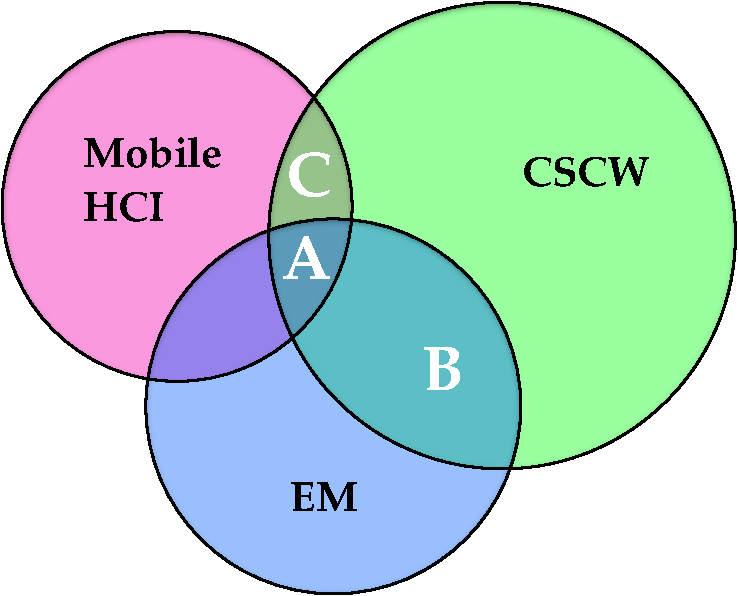
\includegraphics[width=.55\textwidth]{Graphics/1-Introduction/Contributions}
    \caption[Overlap of the different relevant research disciplines and positioning of this thesis' contributions.]{Venn diagram of the influence (size) of the different relevant research areas this thesis draws upon, and how the different multidisciplinary contributions of this work are positioned in relation to each area.}\label{fig:intro contributions}
\end{figure}

% \renewcommand{\theenumi}{\Alph{enumi}}
% \begin{enumerate}

%     \item \textit{Machinery of practices for embedding device interaction in multi-party conversation} --- A praxeological account of the methodical practices employed to embed device interactions in and through contingent social interaction.
%     Furthermore, a rich description of how interacting with devices through visual-touch, voice, and a hybrid-based interface offer and support collaborative efforts amongst members in the setting.
%     This is unpacked and developed through the empirical study and brought together in the discussion (see \ref{sec:synopsis discussion embed}).

%     % \item \textit{Complementing research in existing mental resources literature when exploring non-laboratory use of technology} --- Through the study of interaction with an ethnomethodological analytic lens, this thesis will show how interaction in a non-laboratory setting, such as is the focus of this work, leads to a complex array of interaction modalities being drawn upon and alternated between in quick succession (see \ref{sec:synopsis discussion embed attention}).

%     % \item \textit{Implications for design and study of collocated experiences} --- Based on the study of interaction unfolding with different interaction modes, this thesis will contribute implications for the design and study of collocated interactive experiences, bringing together and juxtaposing the findings from each empirical study (see \ref{sec:synopsis discussion design}).

% \end{enumerate}



% *********************************************************************************************************************



\section{Structure of the thesis}\label{sec:intro structure}
There are \iresubmission{eight} chapters structured over three parts in this thesis, as listed below in \autoref{tab:intro structure}.
A brief summary of each chapter's contribution to the thesis is included in the \textit{Summary} column.

\begin{center}
\vspace{0.5cm}
\begin{longtable}[l]{lp{290pt}}
    \toprule
    \tableheadline{No.}                  & \tableheadline{Summary} \\ \midrule

    \multicolumn{2}{l}{\textbf{\autoref{part:background}: Background and Approach}} \\ \midrule

   \ref{ch:background litreview}     &
   \iresubmission{Continuing the work begun in the Introduction, this chapter lays the groundwork for the thesis by surveying existing literature relating to the use of technology within social and collocated settings, from the perspectives of socio-technical studies, \textit{Mobile \ac{HCI}}, and \textit{\ac{CSCW}}.} \\

   % \ref{ch:background ehf}            &
   %  Relevant literature and theories on interaction modalities, attention, and mental workload from cognitive  perspectives is introduced. \\
    %Although the empirical work undertaken in this thesis does not typically draw on this domain, the findings from this work will be used to contribute new knowledge and practises to \ac{E/HF}, and act as a demonstrator of the contingencies of interaction that an ethnomethodological orientation to analysis reveals.

   \ref{ch:background approach}           &
   \iresubmission{The methodological approach adopted in this thesis is introduced in this chapter.
    Ethnography as a research method is described, and included amongst a brief timeline of the development of ethnomethodological tradition. This provides the context with which the fieldwork and analysis were conducted, and will allow the reader to understand the lens with which this thesis has been produced.} \\ \\
    %The specific practicalities of the approach taken varies based on the particular interaction mode under scrutiny, but the same analytic stance is principally employed in each of the three empirical studies conducted.
    %This chapter will introduce ethnomethodology as a perspective with which the practical and theoretical work in this thesis has adopted, and \ac{EMCA} as an analytic tool used in the orientation to the sequentiality of action of the collected data.
    %This chapter will refrain from practical matters of studying interaction, and focus on the epistemological circumstances of the underlying analysis in this thesis.

    \multicolumn{2}{l}{\textbf{\autoref{part:empirical}: Empirical Work}} \\ \midrule

   \ref{ch:empirical pub}             &
    This chapter presents the study of naturally unfolding interaction with a touchscreen-based portable device within a group of friends socialising together. \\

   \ref{ch:empirical cafe}            &
    This chapter presents a similar study of a group of friends socialising, but where the device interaction is achieved using the \acf{VUI} on the portable device. \\

   \ref{ch:empirical home}            &
    This chapter unpacks how families and friends talk to a \ac{VUI} smartspeaker in the home, with data collected as part of a longitudinal study. \\

    \multicolumn{2}{l}{\textbf{\autoref{part:synopsis}: Synopsis}} \\ \midrule

   \ref{ch:synopsis discussion}       &
    This chapter discusses the findings from the three empirical studies, bringing the findings into the context of existing literature, and how the three independent studies correspondingly reveal the collaborative practices of conversationalists in social settings. \\
    %This chapter will also relate the findings back to the \ac{E/HF} literature uncovered in \autoref{ch:background ehf}, and demonstrate the complexity with which interaction modalities are drawn upon \textit{in vivo}, and the demonstrably need to expand existing knowledge with ethnographic approaches.

   \ref{ch:synopsis conclusions}      &
    This chapter summarises the contributions of this thesis and provides a number of conclusions. \\ \bottomrule

    \caption{Structure of Thesis}\label{tab:intro structure}
\end{longtable}
\end{center}



% *********************************************************************************************************************


\cleardoublepage
\part{Background and Approach}\label{part:background}
%!TEX root = ../PhDThesis.tex



% *********************************************************************************************************************
\chapter{Literature review}\label{ch:background litreview}
% *********************************************************************************************************************



\iresubmission[JR-3b, ER-D: Literature review revised to focus more on detailed studies of technology use]{This chapter introduces existing research on the use of technology while we are engaged in face-to-face interactions with others.}
This literature provides the motivational foundation that led to the development of the research questions posed, as outlined previously in \ref{sec:intro rqs}.
In this regard, this chapter will synthesise the literature that frames the \iresubmission{socio-technical and design} backdrop that informs the current understanding of device use in and around conversation and face-to-face interaction. 
\iresubmission{Understanding how technology fits in and around our interactions with each other, which remains ``the most human thing that we do''~\citep[pp. 3]{Turkle2011}, is the key objective of this thesis.
This literature review introduces work in three key areas in relation to technology use, starting from a `big picture' topic, through to work that this thesis is very much situated amongst: (1) studies of technology use in society, (2) studies of systems designed for collocated interaction, and (3) studies of collocated interaction:}

\begin{revisedsubmission}
\begin{description}
    \item[Studies of technology use in society] \hfill \\
    \iresubmission[JR-3b: This section is new to shift the overall focus onto CSCW studies, but is based upon the previous introduction of work on the Socio-technical perspective]{This first field of work, found in \ref{sec:background litreview society}, unpacks the critically reflective literature on widespread device ownership and use in society from a socio-technical perspective.
    This work examines the role that devices play in public and private settings, such as pubs and the home, and crucially focuses on the \textit{impact} of device use, and people's \textit{reflections} of it, helping to establish the backdrop to which the work in this thesis takes place.}

    \item[Systems design for collocated interaction] \hfill \\
    \iresubmission[JR-3b: This section is new to shift the overall focus onto CSCW studies, but is based upon the previous literature review on Mobile HCI]{This second field of work, found in \ref{sec:background litreview design}, will synthesise literature in which systems are designed for supporting and augmenting interaction with others while we are collocated, with aims to support co-operative working.
    This section will briefly introduce `groupware', before discussing how design work in \acf{HCI} and \acf{CSCW} has moved from  meeting rooms to more diverse settings, supporting new portable technologies.}
    % Early development on ``groupware'' systems~\citep{Ellis1991} coincided with the formation of \acf{CSCW}, with \citet{Grudin1994} detailing how multi-disciplinary foci of the domain to examine practices and design technologies for office environments such as meetings rooms.
    % This later moved out of the home to more diverse settings.
    % Additionally, work began to focus on the design of mobile technologies, such as smartphones, and supporting their use in collocated interaction.

    \item[Close studies of collocated interaction] \hfill \\
    \iresubmission[JR-3b: This section is new]{This final field of work, found in \ref{sec:background litreview f2f}, will introduce detailed studies of face-to-face interaction upon which the methodological approach of this thesis draws.
    This literature seeks to examine device use as a matter of course in and through everyday life, by studying users’ interactions in-the-wild, or rather, \textit{in vivo}.}
\end{description}
\end{revisedsubmission}

By briefly unpacking this literature, this thesis' contribution will be situated as part of this broad and interdisciplinary programme of discourse on the social practices of \iresubmission{technology use in casual-social settings}.
Moreover, this contribution is not based on any theoretical or technical considerations of the design of devices, but on the practices of members in a setting.
As such, this work is \textit{indifferent} to models or theories of interaction (see \ref{sec:background approach em indifference} for an expansion of this point on indifference).
\iresubmission{In this regard, this thesis' focus is on people and how they accountably attend to device use naturally: it is \textit{a study of people and their interaction}, and not technology and its uses.}

This thesis studies three main technological developments: touchscreen smartphones, \acfp{VUI} on touchscreen smartphones, and `screenless' `smartspeakers' that only have a \ac{VUI}.
The commentary in this chapter primarily focuses on portable devices such as smartphones and tablets and includes what little nascent literature exists in relation to `smartspeakers' in the home\footnote{This is, in part, because the devices only became commercially available in the last two or so years of this thesis being produced.}.
%However, the existing literature on the socio-technical study of `conversational machines' will be introduced\footnote{This thesis is intentionally devoid of technical descriptions of `conversational machine' design, which can be found elsewhere, e.g. \citet{McTear2016}, given the focus of this work is on interaction with others around technology use.}.



% *********************************************************************************************************************



\section{Technology use in society}\label{sec:background litreview society}
In this section, a socio-technical perspective of technology use in everyday life is developed to frame the problematic motivational backdrop for the approach and empirical work in this thesis.
The utopian view of how technology is briefly introduced, drawing upon \citet{Weiser1991}'s vision of the computer in the 21st century\iresubmission{, before literature that reveals a \textit{societal impact} of technology use is discussed.
This section then progressively unpacks and synthesises literature that examines and offers a critique of device use, and its `impact' and influence on everyday life.}



% *********************************************************************************************************************



\subsection{Ubiquitous computing}\label{sec:background litreview society utopia}
\resubmission{ER-A, ER-B: This section has been reduced and refocused as a primer onubicomp  only, leaving out the discussions of good/bad device use.}Portable devices take many forms, but presently the most prevalent are smartphones and tablets, which have, for the large part, led the charge in realising \citet{Weiser1991}'s prospective vision of device ownership and ``invisible'' use, as outlined in the introduction of this thesis.
In his work, \citet{Weiser1991} set out a vision of (work) environments, where technology of different shapes and sizes is ubiquitously available and always within reach---its use so finely woven into everyday interactions that it ``disappears''.
This realisation of this is ostensibly led by rapid growth in ownership of smartphones and mobile Internet usage~\citep{Poushter2016}\footnote{The growth of smartphone ownership is remarkable with annual growth rates in ownership of 10\% or higher.}.
\iresubmission{More recent innovations, such as voice-activated `smartspeakers' have also seen rapid growth in the last few years, and can now be found in 32\% of US homes~\citep{AdobeInc2018}.}
%\autoref{fig:background technology weiser}, from \citet{Weiser1991}'s seminal paper, should certainly feel familiar to employees in most work environments.
% One particular technology posed in this work was that of ``pads''.
% These devices, as proposed in the work, will be pervasively available as if they were paper, and we would be able to ``spread [them] around on the desk, just as you spread out papers''.
% In some senses, these devices are not too dissimilar to the commercially-available tablets available of today\footnote{the Apple iPad is an example of a tablet that is similar in size to a stack, or pad, of paper.}.

Yet, of course, the vision is utopian and with all prospective utopian visions, should be treated with caution~\citep{Bell2007}. %---indubitably, the notion that we will make use of tablets candidly as if they were paper may seem fanciful.
However, much of what \citet{Weiser1991} projected bares hallmarks of the reality of today, and as noted by \citet[p. 135]{Bell2007}: ``ubiquitous computing is already here; it simply has not taken the form that we originally envisaged and continue to conjure in our visions of tomorrow''.
Simplistically, it is noted that our work environments feature lots of technology, and owing to the ever-increasing capabilities of wireless communication technologies such as Wi-Fi and Bluetooth, we can interact with devices such as tablets in meetings for multiple tasks.
\iresubmission{Of course, outside of the workplace, technology has also become ubiquitous, thanks to the portability and affordability of smartphones and smartspeakers.
The next section introduces the socio-technical work that examines the use of ostensibly ubiquitous computing devices in society.}
%For example, we readily make use of tablets to send documents digitally to others with relative ease or even hand the tablet around for others to look at.% (c.f. \citet{Luff1998a}).

% \begin{figure}
%   \centering
%   \includegraphics[width=.7\textwidth]{Graphics/2-1-Background-Technology/Ubicomp}
%   \caption[Mark \citet{Weiser1991}'s vision of workplaces in the 21st century.]{\citet{Weiser1991}'s vision for technology in the workplace in the 21st century. This photo shows Computer Scientists at the Xerox Palo Alto Research Centre using multiple different devices, including tablets and a large central screen that the audience is gathered around. This sight is probably familiar to most who work in office environments now.}\label{fig:background technology weiser}
% \end{figure}

% This reality is not quite \citet{Weiser1991}'s vision~\citep{Bell2007}, for several nuanced reasons, and moreover, there remains contention around how much of these propositions have been embraced in the design of currently available devices.
% For example, \citet{Haber2014} challenge the notion that current tablets supplant paper in collocated work environments, irrespective of the increased pervasiveness of tablets (this being one of the key suggestions \citet{Weiser1991} made).
% Through observation, they highlight the nuanced differences in collaborating with and around portable tablets and paper, and in turn demonstrate that people may hold a preference for paper due to qualities that cannot be matched with digital devices.
% Elsewhere, \citet{Plank2017} also found that people had a ``legacy bias'', or \textit{preference}, for using single tablets in interaction, suggesting this vision of ubiquitous, easily-accessible, shared technology has yet to, or might not ever, come to fruition.
% Nevertheless, although \citet{Weiser1991}'s vision seems to be hamstrung by practicalities (such as the cost of devices) and nuanced discrepancies between his projection and the reality, the established opinion is that ubiquitous computing has arrived and that \textit{device use is now embedded in our everyday routine}.
% In this vein, much has been made of the embedded nature of different portable devices and mobile communications on everyday social order, treating devices as ubiquitous and it is this literature that the next two sections review.



% *********************************************************************************************************************



\subsection{Togetherness and isolation}\label{sec:background litreview society together}
There is much praise for the use of portable devices such as cellphones and smartphones, especially with the notion that mobile devices provide or \textit{enhance} our daily lives by helping us to shape our experiences of the world around us, although such critique typically comes with caveats.
Consider social anthropologist Sherry Turkle, for example, who is perhaps one of the most commonly referenced cases.
In her oft-cited work ``Alone Together: Why We Expect More from Technology and Less from Each Other'', which offers a critique of the societal use of technology and weakening `desires' to interact with each other, she finds merit in the unique qualities and ``enhanced experience'' provided by the Internet connectivity of modern devices:
\begin{quote}
    [\ldots{}] connectivity offers new possibilities for experimenting with identity, and particularly in adolescence, the sense of free space, what Erik Erikson called the \textit{moratorium} [\ldots{}] [r]eal life does not always provide this kind of space, but the Internet does.
    \quoteauthor{\citet[p. 152]{Turkle2011}}
\end{quote}
Others have found similar effects, such as notions of togetherness and dwelling established through interviewing participants regarding their use of instant messaging platforms, and specifically WhatsApp~\citep{OHara2014}.
Turkle's praise of technology use remains guarded, however, as she then turns to question the negative effects that mobile device use has in everyday life by noting that, in her view, interactions between people are made problematic by the mere presence and use of devices:
\begin{quote}
    [\ldots{}] face-to-face conversations are routinely interrupted by incoming calls and text messages [\ldots] when someone holds a phone, it can be hard to know if you have that person's attention.
    \quoteauthor{\citet[p. 161]{Turkle2011}}
\end{quote}
\label{line:reclaimingconv}She also extends her criticism of devices in later work by claiming that, with the pervasiveness of devices, we lose the sense of wanting to communicate, and in separate work remarks that we must ``reclaim conversation'' as if it were a dying art form~\citep{Turkle2015}.
This criticism rests on notions that we lose the ability to be empathetic because of our use of technology to mediate communication.
While it is easy to disregard Turkle's problematisation of devices as those of a pessimist\footnote{Indeed, many before her have charged other technologies with a similar critique, e.g. consider \citet{McDonagh1950}'s critique that television has transformed conversationalists in the home into mere spectators.}, her views have held stock in work elsewhere, across different disciplines\iresubmission{, and are, of course, relatable to most people\footnote{In other words, for most people, it is relatively easy to recall a situation where someone was using a device while you were talking to them.}.}

Indeed, numerous surveys and interviews identify the increased portability and functionality of mobile devices as encouraging the acceptability of their use in many settings, such as pubs and social environments.
With this finding comes the implications that the use of devices in public spaces becomes derided and charged as annoying or rude by co-present others, and that interruptions from devices and extended mobile search tasks are a distraction from an ongoing conversation~\citep{Ames2013,Church2012,Campbell2007}.
Contradictorily though, \citet{Ames2013} also identifies through their analysis that ``while students often expected others to be constantly connected, they were not always available themselves''~\citep[p. 1494]{Ames2013}.
\citet{Ames2013}, drawing upon \citet{Turkle2011}'s findings, goes on to highlight the difficulty and ongoing contradiction that exists in relation to device use, as people attempt to balance digital and physical social obligations such as `staying connected':
\begin{quote}
    Many expressed concerns about being tethered to ``electronic leashes,'' able to be yanked at any time out of the present [\ldots] [o]thers adopted the values of those around them: when their families or friends derided them for not being fully present or even just having their phone out, they chose to yield to this social pressure. However, most also felt increased anxiety about what their extended network thought about them as a result.
    \quoteauthor{\citet[p. 1494]{Ames2013}}
\end{quote}
In another case, \citet{Humphreys2013}, also through interviews, highlight findings that suggest that the ease of using the `mobile Internet' potentially exacerbates the problem of ``mis-prioritizing communication through their mobile device over and above face-to-face communication''~\citep[p. 501]{Humphreys2013}.
Additionally, in orienting to the use of mobile devices in public places, and in particular pubs, \citet{Su2015} state that technology can ``threaten conversation by creating the present-but-absent, anti-social, and app-addicted patron''~\citep[p. 1667]{Su2015}.
The next section turns to a specific matter of being connected at all times, in which devices `encourage' their use: device notifications, and the research that has examined their occurrence and influence in our daily lives.



% *********************************************************************************************************************



\subsection{Device notifications}\label{sec:background litreview society notifications}
Moreover, there is a substantive body of work investigating how to `better' deliver mobile notifications to individuals in the face of the potentially disruptive nature of such interruptions from portable devices~\citep{Cutrell2000,Fischer2010a,Lopez-Tovar2015}, and now smartwatches~\citep{Cecchinato2017}, drawing on different methods including the observation of groups completing tasks~\citep{Fischer2013} and conducting contextualised interviews~\citep{Hudson2002}.
Certainly, the existence of such work to tackle interruptions from devices raises the prospect that these interruptions themselves, and the use of devices, in general, led to the issues such as `social isolation'~\citep{Turkle2011}.

This literature on device interruptions should, therefore, establish that many people see the use of technology in everyday settings as \textit{problematic} and \textit{disruptive}, in part because their use is brought about by interruptions \textit{arising from} devices.
But, for example, multiple studies have established that although interruptions from devices, such as notifications,  are characterised as problematic, many still prefer to receive notifications than not, for myriad reasons, \iresubmission{including ``awareness''~\citep{Iqbal2010} and to avoid the feeling of ``being cut off''~\citep[p. 560]{Mark2012}}.
\citet{Pielot2015a}, by asking participants to disable notifications on their devices for 24 hours and interviewing them afterwards, identified that ``many participants were anxious to miss information from significant others and superiors''~\citep[p. 1765]{Pielot2015a}.

In reading this literature, it becomes clear that the accepted view is that there are also positive perspectives in relation to the portability and flexibility of mobile devices.
This advantage allows for their greater use within many different settings, including conversation, and allows such devices to provide a utility in which people can remain in touch with their extended network.
This raises expectations that we should quickly respond to our contacts from our friendship groups, just as we expect them to respond~\citep{Ames2013}.
This immediacy provides users with the sense of being ``always connected, to be accessible at all times and places''~\citep[p. 240]{Peters2005} and removing the ``binding between a fixed space and a person’s information and communication resources''~\citep[p. 324]{Perry2001}.
It seems that people find device use problematic because of the burden of managing constant availability~\citep{Sadler2007}, yet find it indispensable and the notion of `untethering' as undesirable because of this very same quality.

Even regarding `non-notification-instigated' use, devices are identified as potentially being a \textit{beneficiary} to everyday life in the home.
For example, \citet{Lanigan2009}, in a study of the use of technology in family life, had what they even considered a ``surprising finding''.
The research found that ``that the more time families spent engaged with the computer, the higher their level of communication, cohesion, and adaptability'', with a home computer encouraging ``more frank communication'', an increase in ``family time [\ldots] due to efficiencies gained through computer use'', and ``a source of mutual interest'' for the family~\citep[p. 603]{Lanigan2009}.
It seems, then, that devices are likely to remain present in our everyday social interactions.
The next section progresses on to examining literature that unpacks how our experience of space is shaped by this device use.



% *********************************************************************************************************************



\subsection{Device use and space}\label{sec:background litreview society space}
Furthermore, exacerbating this point, the use of mobile devices in public settings has been well documented in literature for a variety of purposes, from how an iPod allows an individual to reshape their experience of time and space~\citep{Bull2005}, to how individuals use new technologies such as cellphones to adapt their social perspective~\citep{Humphreys2005,Oksman2004,Peters2005}, and to the enjoyment and ludic pursuits people explore with devices~\citep{Brown2015a}.
In relation to how we now make use of devices anywhere and everywhere we go, \citet{Geser2006} presents a sociological review of whether the mobile phone is `undermining social order'.
He concludes that, through review of how `time-based scheduling and coordination' has declined because of the ready availability of devices, ``a new, more fluid culture of informal social interaction therefore can emerge''~\citep[pp. 5--6]{Geser2006}.
Furthermore, \citet{Campbell2008} argue in an essay that ``mobile communication around copresent others [\ldots] personalizes the communal experience of being in that space''~\citep[p. 379]{Campbell2008}; which also supports work by others of the practice of using technologies to create private spaces in public places (e.g. \citet{Ames2013,Wei1999}).

This literature, which draws on different approaches, establishes that given the desire, or in some cases, compulsion, to remain connected, there is a need to understand the complex factors around the co-management of both the virtual and physical interactions.
This is, in part, due to the relative ease for individuals to retreat to their phone and ``shield oneself from wider surroundings''~\citep[p. 4]{Geser2006}\iresubmission{, which may unfold as individuals with anxiety use the device to shield themselves from unmanageable situations~\citep{Wei2006}}.
Thus, the fact that mobile devices are always connected, and that devices can provide notifications at any point, a situation may become engendered where virtual interactions can potentially rub up against collocated physical interactions.

% These factors all bring to the fore the nuanced and complicated nature of characterising device use as troublesome, as device use, in all forms, is found to provide upsides as well as downsides.
% For example, smartphones have many obvious benefits, such as allowing people to remain in touch with loved ones while away and for calling emergency services whenever they are needed.
% Perhaps not so obvious, there are also situations where devices are used by people with medical conditions for various purposes.
% Furthermore, they allow those who are anxious to shield themselves from unmanageable situations~\citep{Wei2006}.
% Devices are also used as fitness and health trackers, and with connected smartwatches as tools to detect and monitor health conditions such as hypotension and sleep quality~\citep{Phan2015,Iakovakis2016}.
% This review must not be confused as a critique of such research, but instead demonstrates that many of the arguments surrounding device use are well-rehearsed, revised, and challenged within literature.

However, many of these arguments are derived through sociological critique or interviews, opening a gap in the literature for an examination of device interactions from an observational perspective.
Such a perspective avoids being caught up in narratives of perception and feeling, instead orienting researchers to the observable matters of device use, to identify specifically what is \textit{practically done} when people use a device in conversation.



% *********************************************************************************************************************



% \subsection{User experiences of using devices}\label{sec:background litreview society experience}
% %Given the difficulty in capturing `everyday use', many studies default to unpacking the intricate details of device use through interviews and/or diary studies.
% % Both approaches rely upon self-documentation and recall.%\footnote{Anecdotally, my experience of diary studies is that most people complete the diary some time after the event they are recording.}.
% % The strength of such approaches is that through careful interviewing recall is imbued with critical self-reflection and information, and insight into user experiences of device use can be captured over periods of time that would otherwise be difficult to observe~\citep[p. 273]{Wilson2015}.
% % However, such approaches cannot reveal the practical details of how interaction unfolded from an intersubjective perspective~\citep{Berger1966}\footnote{Intersubjectivity is a notion that sidesteps the objective-subjective dichotomy of research, and features heavily in ethnomethodological perspectives because these studies observe practice that is observable and reportable --- such observations are neither objective fact or subjective interpretation (it is not a matter of opinion that someone does something). In other words, intersubjectivity is the acknowledgement that what is done is seen and understood by those who have the competence to see and understand it.} of naturally accountable actions within the setting.
% % Furthermore, many of these studies orient to such devices as \textit{novel devices}, and not devices that are embedded within the lifeblood of mundanity.
% In addition to understanding the reflections of device use, others have turned to matters of the  user experience of using the devices.
% Given the difficulty in capturing `everyday use', many studies default to unpacking the intricate details of device use through interviews and/or diary studies.
% One of the first studies to examine smartphone use identified the `mess' of the multi-functionality of these devices, and of how they differ from \citet{Weiser1991}'s vision by remaining `personal', unpacking issues of seamfulness~\citep{Barkhuus2011}.
% This work, as with others, was completed through interviews and diary studies.
% \citet{Su2015} also relied on interviews for producing their findings\footnote{Although the study also includes observations, the findings were constructed out of interview data.} of mobile device use in Irish pubs, who identify how the presence of mobile devices transform pubs into ``surveilled places'' where individuals could no longer assume privacy.
% Both of these studies find benefits and downsides of existing smartphones, as discussed above in \ref{sec:background litreview society together}, but what they lack is concrete descriptions of how such interactions unfold, and instead default to scenic descriptions of activities that unfold, e.g. ``[s]everal users had ``weird fact'' apps that generate random trivia they would read out loud to friends—essentially, a conversation generator.''~\citep{Su2015}.
% While such findings furnish researchers with an understanding of the sorts of activities that unfold, they are limited in their usefulness in providing valuable and actionable implications for design.

% \citet{Luger2016}, in what was one of the first studies of `modern' commercially-available \acfp{VUI}, interviewed participants about their experiences of such interfaces.
% Manufacturers pitch these devices as being able to handle a complex range of tasks, driven by input through voice.
% This study, as above, used interviews for critical reflection to find shortcomings with existing voice interfaces on smartphones, and that the features of the devices were promoted in such a way that a ``gulf'' formed between expected functionality and that of reality.
% \citet{Luger2016} were remarkably succinct in generating a wide range of actionable implications for design, but because of the approach still provided little in the way of empirical description of the methods of use done by participants, instead relying upon commentaries by participants for revealing the technical troubles that occur.
% Although their findings are useful as a mechanism for honing in on potential problems with interfaces, they do not provide fine-grained detail used to reveal the social organisation of such device use in a casual-social setting, or while collocated with others.



% *********************************************************************************************************************



\subsection{Summary}\label{sec:background litreview society summary}
This brief introduction should highlight and synthesise the examinations of technology use, especially from the perspective of the `impact' of the use of technology in everyday life.
Crucially, this work draws upon reflections, interviews, and sentiments about how technology is used.
\iresubmission{While this thesis adamantly does not dismiss the validity of such findings---indeed they tell us a lot about the world we inhabit---much of it does not examine how device use \textit{practically} unfolds, as \textit{situated action}~\citep{Suchman1985}, and in doing so loses its ``utility in design'' that ethnography, and specifically ethnography informed by ethnomethodology, proffers~\citep[pp. 879--880]{Crabtree2009}.}

In the context of this thesis, then, it is pertinent to consider that as individuals gather to socialise, device use can impact an individual's orientation to space and other co-inhabitants.
This thesis does not adopt a moral or sociological critique of this use but draws upon this multi-faceted argument to consider the rudimentary notion of how such interactions practically unfold (i.e. \textit{what do people actually do with their devices?}). %\footnote{This was a question posed to me after presenting the general premise of this research. I stood at the front of the room shell-shocked by this question, and answering it took three and a bit years.}).
As opposed to attempting to gloss the use of mobile devices to generalisable problems or benefits, or relying upon reflections and interviews to guide understanding, this work is interested in explicating the unfolding and nuanced nature of this practice, as it happens \textit{in vivo}, and how it can be used for design.
This thesis will add to this existing debate by addressing a gap in literature through the provision of \textit{empirical data} that reveals the interactional work people do to use devices in and through interaction.
The next section introduces academic and design efforts to build technologies that support existing collaborative efforts as well as supporting new collaborations using portable technologies.



% *********************************************************************************************************************



\section{Systems design for collocated interaction}\label{sec:background litreview design}
\iresubmission[ER-1 JR-1, IR-2: Include additional literature from CSCW]{This second tranche of literature introduces the long-standing focus of designing systems that allow multiple co-present users to work together under the label of `groupware', originally primarily addressed in \ac{CSCW}.
More recently this work has moved out of the office settings and become concerned with other public and private settings, and examining both sedentary and \textit{mobile} device use.}
With this, the work now spans the overlapping disciplines of \ac{HCI} and \ac{CSCW} (as does this thesis).
\ac{HCI} is perhaps best described as an ``eclectic interdiscipline'' that was initially primarily concerned with notions of the \textit{user experience} of technology, although now encompasses ``all aspect of human life, from birth to bereavement, through all manner of computing, from device ecologies to nano-technology''~\citep[p. vii]{Rogers2012}.
%It is a result of this that \ac{HCI} research is itself interdisciplinary, and draws many different well-established disciplines including psychology, sociology, design, \acf{E/HF}, and so on.

Research in this area has many interchangeable labels, such as collocated~\citep{Lucero2013}, co-located~\citep{Jarusriboonchai2014}, or co-present~\citep{Cole2003} interaction, and same-time same-place~\citep{Fischer2016} research, although here the first of this list is selected for consistency with publications supported by the work in this thesis.
Essentially, in each case, the premise is identical in that work examines the use of technology in situations where there are two or more people present.



% *********************************************************************************************************************



\subsection{Groupware}\label{sec:background litreview design groupware}
\begin{revisedsubmission}[ER-1 JR-1, IR-2: Include additional literature from CSCW]
Early work in \ac{CSCW} examined how to develop groupware systems~\citep{Ellis1991} and other systems to support multiple co-present users interacting with technology and working together, often also referred to as \textit{collaborative software}.
Primarily, technologies were designed for workplace settings such as meeting rooms that were already sites for collaborative action.
Groupware as a term covers a range of software---from supporting collocated interaction and meeting facilitation, e.g. slideware~\citep{Chattopadhyay2018}, through to technologies to support distributed working, such as email-based technologies.
The motivation behind the development of groupware systems was not just the increasing availability of technology during the 80s and 90s, but also the potential benefits of augmenting existing practices with technology.
For example, systems designed to support decision making were found to \textit{increase} decision quality and equality of participation~\citep{Olson1993}.

Progressively, the settings which collaborative systems were designed for moved ``out of the meeting room''~\citep{Bergqvist1999} to classrooms~\citep{Abowd2010}, museums~\citep{Ciolfi2003}, public spaces~\citep{Reeves2011}, air traffic control~\citep{Hurter2012}, and the home~\citep{Edwards2001,Crabtree2016}.
In addition to new spaces, new technologies became the focus of new interrelated fields, such as tabletop interactions and interactive surfaces~\citep{Gjerlufsen2011,Jones2012} through to mobile devices~\citep{Bellotti1996},  such as smartphones and tablets~\citep{Lucero2012}.
It is the latter of this list that the next section focuses on---this field of work, sometimes referred to as \textit{mobile collocated interactions} or part of the field of \textit{Mobile \ac{HCI}}, is occupied with designing technologies for interactions with personal devices while we are collocated with each other, i.e. the situation for which this thesis seeks to understand the social organisation.
\end{revisedsubmission}



% *********************************************************************************************************************



\subsection{Mobile collocated interactions}\label{sec:background litreview design mobilehci}
This section introduces work from the domain of `Mobile \ac{HCI}'.
There is a duality to the definition of mobile in the sense of `Mobile \ac{HCI}', in that it refers to interaction and physical mobility; or the design and use of mobile devices and mobile device applications, i.e. \textit{portable} devices but in potentially sedentary settings~\citep{Church2011}\footnote{Other work also adopts differing definitions of \textit{mobility}, for example, \citet{Luff1998a} use the term in relation to the micro-mobility of artefacts in face-to-face interaction.}.
The work in this section focuses on this latter definition, considering literature that explores interaction in \textit{collocated settings}, i.e. when multiple people are physically collocated together in the same setting, and often sedentary, but use portable technologies such as smartphones and tablets.



% *********************************************************************************************************************



Mobile \ac{HCI} literature is replete with use cases of collocated mobile device interactions, spun out of academic-led design work, such as photo sharing~\citep{Counts2004,Durrant2011}, video watching~\citep{OHara2007}, and collaborative searching tasks \citep{Church2012,Cole2003,Brown2015}, and often involving interaction with additional screens or multiple mobile devices~\citep{Bergstrom-lehtovirta2013,Lucero2013}.
This literature implicitly attempts to demonstrate the beneficial uses of technology in collocated interactions, which expediently refutes---or at least qualifies---simplistic popular views that mobile devices create `social isolation'~\citep{Turkle2011}.
The growing body of literature is exemplified through the generation of design frameworks for the curation of collaborative collocated experiences with technology (e.g. \citet{Lundgren2015}).
In this, mobile devices are examined as artefacts that can be brought into everyday cooperative interactions, with the work of designers transforming their ``features and functionalities [\ldots] into resources for action''~\citep[p. 1117]{Salovaara2007}.

\label{line:singleuser}Much of the work within collocated interactions literature, as a subset of existing Mobile \ac{HCI} research, has challenged the \textit{single-user} nature of \textit{personal} devices, to provocatively explore how the use of mobile devices could instead be designed as \textit{shared} devices that support \textit{multi-user} interaction. This is best elaborated in an \textit{interactions} article on \textit{`Mobile Collocated Interactions'}:
\begin{quote}
    When using their mobile phones, people have a tendency to hold their devices with one or two hands, with the screen facing toward them. People will usually adopt a particular device position, combined even with a second hand to cover the screen, either to browse private content, such as a confidential email, or to avoid glare [\ldots] For people to fully benefit from mobile collocated interactions, they must open up and start seeing their personal devices as shared, public devices. In mobile collocated interactions, phones are at the intersection of fully personal and fully shared use.
    \quoteauthor{\citet[p. 28]{Lucero2013}}
\end{quote}
Many examples of this work, which seems to hark back to elements of \citet{Weiser1991}'s vision\footnote{
Indeed, the notion of devices switching from `personal' to `shared' use is an embodiment of this vision.} (see \ref{sec:background litreview society utopia}), operate by adopting existing \textit{implications for design} from previous studies to guide the design work of a new prototype.
The prototype developed within mobile collocated interactions research is typically tested with `real-world' users in a field trial (e.g. \citet{Lucero2012}), and the resulting analysis used to generate new implications for design.
Some work also specifically follows routes of creating provocative prototypes, not to solve users' problems, but to find ways of evoking critical reflection by users~\citep{Redstrom2006}.
For example, \citet{Lundgren2013} explore ideas to ``design interventions that investigate how apps for mobile devices can make people interact directly in co-located space instead of enclosing themselves with their own digital device''~\citep[p. 1]{Lundgren2013}, primarily using the idea of games to prompt users to reflect and consider interacting with collocated others.

In the same spirit of creating enjoyable interfaces. but with the idea of using the device as a ``resource'' for conversation, \citet[p. 232]{Porcheron2016b} explored the idea of allowing individuals to collect and share photos and notes for a design project with their mobile phone.
The app allowed users to collocate and share the collections but fundamentally required the group to converse face-to-face with each other to use the application successfully and navigate its features.
This work, along with others such as \citet{Lucero2012} that allowed for large display and cross-device interactions in public settings from mobile phones, provides a semblance of supporting the notion that device interactions can be curated, can be enjoyable~\citep{Brown2015a}, and can be used to enhance people's experiences of space (e.g. as in \citet{Bull2005}) and conversation with each other (e.g. \citet{Lundgren2013}).



% *********************************************************************************************************************



\subsection{Designing the context-aware device}\label{sec:background litreview design mobilehci context}
Related to this, the notion of designing for space and the context within which the device is used is explored elsewhere, with a considerable body of work that looks to make device interactions more sensitive to their environment and context of the world around the device.
For many years, a holy grail of Mobile \ac{HCI} research was the ``context-aware''~\citep{Schilit1994} smartphone, with many designs explored in literature; one such influential example is `ContextPhone' by \citet{Raento2005} although there are many more (e.g. \citet{Siewiorek2003,Gellersen2002}).

The purpose of this research is to establish ways of making devices sensitive to the environment, with \citet{Gellersen2002} drawing on \citet{Weiser1991}'s vision to note that ``[i]n the mobile device user interface, context can be used to facilitate a shift from explicit user-driven to implicit context-driven interaction''~\citep[p. 341]{Gellersen2002}.
In the frame of the `contextually aware device', the view of what \textit{context} is differs perhaps from the sociological or interactional definitions, and is broadly classed as:
\begin{quote}
    [\ldots] any information that can be used to characterize the situation of an entity. An entity is a person, place or object that is considered relevant to the interaction between a user and an application, including the user and applications themselves, and by extension, the environment the user and applications are embedded in.
    \quoteauthor{\citet[p. 217]{Dey2009}}
\end{quote}
The ambitions to create devices that are sensitive to anything that is `relevant to the interaction' have generated numerous design and research challenges.
Many of these ideas draw on the notion that context can be used to ameliorate problematic interactions with devices, and are spurred on by the critique that devices are invasive in everyday life (see \ref{sec:background litreview society}).
One of the practical ways in which notions of ``contextual awareness'' have been realised in research is through notification sensitivity to the environment, i.e. a device will determine when to deliver a notification at the ``opportune moment''~\citep[pp. 57--64]{Fischer2011}.
Work in search of the contextual device has progressed, and has considered and explored design ideas for reducing the impact of notifications on many different portable devices such as smartphones (e.g. \citet{Okoshi2016}), smartglasses (e.g. \citet{Kern2003,Lucero2014}), and smartwatches (e.g. \citet{Lee2016a}) by withholding notifications until a later time.

%Progress in this space is swift and is driven forward by the rapid growth in mobile computing power and sensing capabilities.
\iresubmission{Furthermore, ideas also surround the use of the `continuous speech stream' in design to detect the context.
In other words, devices which listen to the stream of speech around them would make use of a continuous and live transcription of conversation to prepare or sensitise interactions to the context~\citep{McMillan2015}.}
In a prototypical trial of this, \citet{Schulze2016} found their system to be on-the-whole suitable, but then attach caveats that ``if conversational context is employed to determine interruptibility, the prior characterization of the conversation is essential'' and ``concerns of participants that go beyond our measures to preserve privacy and beyond a lack of their being informed about those measures, can’t be addressed by design''~\citep[p. 9]{Schulze2016}, exemplifying that the challenges of the context-aware smartphone are socio-legal as well as technical.

However, in spite of this progress addressing the challenge of devices that tailor their interactions to our setting, manufacturers have been slow to adopt such features.
Some smartphones feature options that enable a silent mode when they are placed face down; however, typically devices defer to the user to configure settings for notification management.
The result of this is that the decision of when to deal with interruptions from a device is left to the user.



% *********************************************************************************************************************



\crpagebreak\subsection{Summary}\label{sec:background litreview design mobilehci summary}
\iresubmission{This section has established the tradition of designing systems to support co-operative working within \ac{CSCW} and (Mobile) \ac{HCI}.
Progressively, the focus of development expanded from meeting rooms through to other settings and technologies, including mobile settings \textit{and} mobile devices.}
The literature on creating collaborative experiences with mobile devices while we are collocated with others was summarised.
Then literature was introduced that examines the parallel efforts to ameliorate the problematised nature of device-triggered interruptions to create mobile interfaces that are sensitive to `contextual' information.
Although notifications play a big part of `life with devices', it is expected that they form only part of the occasioning of devices in social settings.
This is reinforced by~\citet{Sohn2008} and \citet{Church2008}, whom both used diary studies to reveal other many reasons for the use of the Internet on a portable device beyond mere device-instigated notifications.
The next section will pivot from matters of designing technologies to studies of how mobile devices are used in everyday life, from a perspective focused on close studies of face-to-face interaction.



% *********************************************************************************************************************



\section{Close studies of collocated interaction}\label{sec:background litreview f2f}
\begin{revisedsubmission}[ER-1, JR-1, IR-2: Include related CSCW literature]
This final section will synthesise the literature that examines interaction amongst people while they are face-to-face, especially from the \ac{HCI} and \ac{CSCW} domains.
These are typically `close' studies of interaction, i.e. they take an approach that orients to observable matters of technology use to address specifically what is practically done when people use of technology `in the wild', with empirical data being the commodity that establishes the findings of the work.
The first section will discuss the \textit{turn to the social} in \ac{HCI}.



% *********************************************************************************************************************



\subsection{\textit{Turn to the social} in HCI}\label{sec:background litreview f2f turn-to-the-social}
\citet{Suchman1985}'s work represents some of the earliest and oft-cited work in \ac{HCI} on the study of the social organisation of interaction with technology in this vein.
Her work, undertaken in a lab-based setting, examined the use of agent-based photocopiers, adopting ethnographic approaches and drawing on the ethnomethodological perspective (this is unpacked later in \autoref{ch:background approach}).
This work was undertaken in parallel to other key works in \ac{CSCW} studies around the same period which examined settings such as air-traffic control rooms~\citep{Bentley1992}, drawing upon similar perspectives, to unpack the cooperative working practices in order to support design activities~\citep{Bannon1993}.
The domains of \ac{CSCW} and \ac{HCI} were increasingly focused on studies of control rooms; in a range of settings from \citet{Heath1992} in a London Underground control room, \citet{Goodwin1996} in air traffic control rooms, and \citet{Watts1996} in NASA mission control rooms.
\citet{Suchman1997} characterised such settings as ``centers of coordination'', in which ``participants' ongoing orientation to problems of space and time'' is crucial in attending to matters of deployment of people and equipment in response to a planned timetable or emergent requirement~\citep[pp. 41--43]{Suchman1997}.

As discussed above in relation to design efforts shifting out of meeting rooms, ethnographic studies too shifted ``out of the control room'' and other constrained settings~\citep{Hughes1994}, as part of a ``turn to the social'' in \ac{HCI} and \ac{CSCW}.
This turn was ``a primary point of view for analysing the design space under the auspices of groupware and cooperative systems''~\citep[p. 28]{Crabtree2003a}.
In this regard, the practice of studying interaction in constrained settings became re-purposed for examining matters of ``everyday life''.
The next section introduces literature that details studies of face-to-face interaction and technology use.
Suchman's work, and that of the Lancaster \ac{CSCW} studies, transformed the ethnographic practices, and the use of the ethnomethodological perspective, into utilities for design in \ac{HCI} and \ac{CSCW}.
This transformation of studies for design did so to support adoption of an ``analytic orientation to fieldwork, which seeks to uncover the locally organized character of action and interaction [\ldots] [that is] is essential to the ongoing development of computing systems that resonate with, support, and enhance what people actually do in new design contexts and how they organize what they do''~\citep[p. 881]{Crabtree2009}.
The next section will synthesise and discuss the literature from \ac{HCI} and related disciplines on the use of technology while we are collocated with others.
\end{revisedsubmission}



% *********************************************************************************************************************



\subsection{Using technology while collocated}\label{sec:background litreview f2f tech-while-collocated}
Early observational studies of portable device use\footnote{Note that these studies were conducted in the early 2000s before the widespread commercial availability of smartphones, and thus they are studies of what may now be considered `traditional' mobile phones, or cellphones, or non-smartphones.} examined aspects such as how devices were shared amongst groups of friends.
For example, \citet{Weilenmann2002} discuss a study of young people in Sweden making use of phones, with observations collected anonymously in public spaces focusing on how sharing is done between collocated friends.
Elsewhere, \citet{Murtagh2002} describes the grossly observable features of mobile phone use during observations of people on train carriages. %, while \citet{Edwards2001} examine aspects of ubiquitous technologies in the home and what it is to `live with them'.
%Both of these studies draw upon an ethnomethodological perspective, as adopted with this thesis (explained later \autoref{ch:background approach}).
\citet{Krehl2013} followed travellers on public transport journeys and categorised their mobile device use.
This categorisation and resulting model was based on contextual factors relating to the use of devices---such as location, task, and technical details.
Such findings provide a comprehensive insight into the activities of device users while mobile, again, providing rich, actionable foundations for work to design a contextually sensitive device (see \ref{sec:background litreview design mobilehci context}).
Conversely, through the collation of existing literature, \citet{Nakamura2015} presents a model of the actions people employ in looking at mobile phone displays in everyday life as non-verbal communication, bringing to the fore some nuanced and complex issues around mobile device use in public life.
This work positions the ``phone user behind something akin to the `fourth wall'''~\citep[p. 74]{Nakamura2015}, which while beneficial for making sense of generating generalisable models of interaction, also does the work of detracting from the situated and contextually-shaped (and contextually-shaping) nature that interaction with a mobile phone occasions and is occasioned by (discussed later in \ref{sec:background approach em sequentiality}). 
%However, these pieces of work do not examine device use moment-by-moment, inste by orienting to the sequentiality of action (see \ref{sec:background approach em}) and shows that, far from being enacted outside of the social sphere, is directly embedded in and through the activities of the users.
%\citet{Brown2014}, in a separate analysis, go on to quantify that 25\% of their captured video ``involved a conversation that took place around the activities on the smartphone'', rubbing up against the notions that ``human relationships are still in decline'' because of the presence and use of devices~\citep{Slade2012}.

\iresubmission{There is also a growing body of work that reveals the intricate ways in which device use becomes interleaved in a variety of settings, adopting methodological approaches that examine interaction moment-by-moment, ranging from kitchens~\citep{DiDomenico2013} and living rooms~\citep{Rooksby2015} through to collaborative photo-taking activities~\citep{Fischer2013}. 
On people using mobile devices while watching television, \citet{Rooksby2015} remark that ``[w]e should not view the mobile device as being brought into television viewing, but the use of mobile devices, the watching of television, and so on as things being brought into leisure''~\citep[p. 17]{Rooksby2015}. 
The sense here is that the use of mobile devices is part of leisure activities in the home, rather than an isolatable activity.
In another study that recorded and studied participants use of smartphones over an extended period, the authors identified how 25\% of all portable device interactions took place while participants were co-present with others~\citep{Brown2014}, illuminating the notion of how the use of devices routinely occurs while we are around others.}
Through the use of screen-recording and fitting participants with portable ``camera bags'', \citet{Brown2013} provide  empirical and rich insight into the daily use of smartphone users.
The work also goes on to introduce sequential practices of how devices are occasioned through activities such as route finding and how web searches are initiated: by others in talk, by events taking place, and by features of the local environment.
The research also brings to the fore how people make use of multi-modal features (e.g. gaze, orientation) to use the device in conversation with others successfully.
\citet{Pizza2016} follow a similar modus operandi to capture the use of smartwatches, revealing what smartwatches are used for and that people embed the interaction with the smartwatch in conversation, which they demonstrate through detailing ``users’ everyday activity [\ldots] [in one situation] the participant is talking about last night, arranging some ingredients for cooking, and quickly reading a notification on the watch''~\citep[p. 5464]{Pizza2016}.
This attention to the minutiae of interaction provides a detailed and rich insight into the interactional accomplishments of people, as they embed device use in other ongoing activities.

\begin{revisedsubmission}
Furthermore, as \citet{Isaacs2012} remark, ``people attempt to blend their local and remote worlds into
coherent interaction when sharing content and one experiences with friends through their devices [and that these] behaviors are becoming more varied, and possibly more common, because of the prevalence of ubiquitous devices and bite-sized content''~\citep[p. 625]{Isaacs2012}.
Work in \ac{HCI} and \ac{CSCW} establishes the case that device use becomes embedded within and is treated as part of activities in everyday life, from television watching~\citep{Rooksby2015} through to searching the web, as occasioned in and through conversation with co-present others~\citep{Brown2015}.
These practices include people embedding the device in interaction through collaborating on web searches~\citep{Brown2015} or making the screen visible to others during use~\citep{Raclaw2016}.

Overall, these studies took place by observing people `in the wild' naturally (i.e. by orienting to
the naturally accountable methods in which members socially organise their interaction), with the studies taking place in perspicuous settings~\citep[pp. 181--182]{Garfinkel2002} to the technology being considered.
This is not to say that such settings could not be constructed as part of the research, for example as laboratory settings~\citep{Rooksby2013}\label{line:labsettings}, and it is the defence of such studies by \citet{Rooksby2013} that is crucial to this thesis: ``[i]f there is to be a ``turn to the wild'' in HCI, this should not be a turn away from the laboratory but a turn away from research methods that ignore human practice''~\citep[p. 1]{Rooksby2013}.
In other words, the \textit{turn to the social} is not, per s\'{e}, a preference for conducting studies outside of laboratory settings, but ones in which the social organisation of the setting and the members within that is crucial to design~\citep{Crabtree2009}, is the locus of the researcher's concern.
Any study that seeks to examine interaction and technology use for design must attend to the matters of the social organisation of the setting as such details ``[\ldots] matter and not as analytic phenomena'' but as matters which the members of the setting understand and must be designed for~\citep[p. 137]{Crabtree2012}.
This thesis takes a hybrid approach, insomuch that the participants are recruited for research and asked to attend a social setting, but the setting is one which they would typically visit together for a research study, and is of perspicuity for the technology interaction of concern.
Participants were made aware that interaction around device use was being studied in each case, with the second study asking participants to preferentially use the \ac{VUI} on their smartphone instead of the touchscreen and the third study including the provision of the technology as part of a deployment to participants' homes.
The focus of the work in this thesis is \textit{the naturally accountable ways in which members attend to device use as it unfolds }(i.e. to reveal \textit{how} it unfolds), and not to establish \textit{why} device use unfolded.
\end{revisedsubmission}

Indeed, most studies of voice-based interfaces have, partly for technical reasons, consisted of Wizard of Oz studies in which the `computer' or \acf{VUI} has been driven covertly by a human rather than a computer agent, in effect introducing a simulated element to the interaction\footnote{This is not to say that such an approach would impede a study of attending to the social organisation of device use; indeed, it is argued as much on page \pageref{line:labsettings}. This is merely to remark that there are nascent studies of commercially available \acp{VUI}.}.
Such practices are long-standing with \ac{VUI}-design related work and studies, with early research on simulating \acp{VUI} used to demonstrate or provide software to implement such studies~\citep{Klemmer2000} or how to undertake a conversation analytic approach to analysing such interactions~\citep{Fraser1991,Wooffitt1994,Wooffitt1997}.
Specific examples also include studies such as how \acp{VUI} can be sensitively designed for use in safety-critical situations such as during driving~\citep{Martelaro2017}, for use in mixed-reality games~\citep{Dow2005}, and action games~\citep{Hoysniemi2004}.
These authors all show how members make use of devices precisely, alter their voice for the device~\citep{Pelikan2016}, and manage the interaction so that it unfolds when opportune~\citep{Martelaro2017}.
Furthermore, each one adopts the perspective of analysing situated action, to reveal details of how users attend to the devices in a particular context, eschewing notions of a generalisable model of interaction.
These studies demonstrate the suitability of adopting observational perspectives to studying device use in order to reveal nuanced interactional practices, but also demonstrate the relevance of studying device use in a particular context---it is not possible to transgress findings from studies across different contexts.
\iresubmission{Given the recent commercial availability of \acp{VUI} on smartphones and standalone \ac{VUI} devices, the necessity to study interactions with them through the Wizard of Oz technique is mitigated, however, the work in the latter two chapters remains among the first to study the social organisation of the use of actual systems in the wild.}



% *********************************************************************************************************************



\subsection{Summary}\label{sec:background technology vivo summary}
This section has introduced literature that has studied the lived experience of device use \iresubmission{through observational studies.}
This work, in juxtaposition with the design work in mobile collocated interactions (see \ref{sec:background litreview design mobilehci}) that intentionally prototypes designs for precisely these \textit{sorts} of settings, demonstrates a shortcoming in literature.
\iresubmission{This section has brought together literature that has examined collocated interaction while mobile and sedentary, with different devices such as smartphones and smartwatches.
However, at the time the work was conducted, there was no study of how device use unfolds in social settings such as public places like a pub, which bring with them `certain ways of behaving' given the specificity of the setting (discussed later in \ref{sec:empirical pub design setting}).
Furthermore, there remains nascent literature on the use of smartphone-based \acp{VUI} and smartspeakers given the recency with which they were introduced, with most studies to date consisting of Wizard of Oz-based studies.
The empirical work in this thesis will address these gaps.}

\begin{revisedsubmission}
The turn to the social in \ac{HCI} centred around the import of ethnographic practices and the ethnomethodological perspective.
This expansion of ethnographic practices into \ac{HCI}, in turn, allows research to support design efforts by generating significant implications for design, which as \citet{Crabtree2012} remind us, allows designers to ground decisions in `facts'~\citep[p. 137]{Crabtree2012}.
Although it is not the purpose of this thesis to design new technologies, through the documentation of the social organisation of conversation with technology interleaved, a greater understanding of how future technologies could meet the needs of users could be designed.
\end{revisedsubmission}

% Therefore, this thesis unpacks interaction as-it-happens in a collocated casual-social setting, without defaulting to simulated or interview-based studies, and will instead present rich empirical data of interaction as its core finding.
% The studies of touchscreen devices in social settings in this thesis follow on from early \ac{CSCW} work on the micro-mobility of documents~\citep{Luff1998a}.
% This work unpacked how documents on paper are used, shared, and passed around in the process of collaborating together for work-related tasks.
% It is in this spirit that this thesis will show how people use and share mobile device interactions in a similar fashion, to collaborate on activities that are occasioned in and through conversation (see Chapters \ref{ch:empirical pub} and \ref{ch:empirical cafe}).
% The last study continues in the same vein, while studying speech-only interactions (\autoref{ch:empirical home}), but again, uses actual empirical data as the bedrock for the findings, instead of simulating interaction with a computer.

%The interests of this thesis lie in how individuals manage the use of these `always connected' devices in conversation, the observable-and-reportable actions of those in the setting, and just \textit{how} device use is embedded in the social order and enacted in and throughout the ongoing interaction.
%Thus, this thesis is interested in attempting to understand the specific interactions that occur, and how devices become occasioned during a conversation, and how their use is embedded in everyday talk.
% Insights in this space have the potential to help designers with the goal of creating more fluid device interactions for multiple users, allowing others to take into account the uncovered interactional practices in their own future work.
% As such, these studies will build upon literature that empirically examines device use \textit{in vivo}, and more fundamentally, present one of the first studies of \textit{\acfp{VUI}} in-the-wild.



% *********************************************************************************************************************

%!TEX root = ../PhDThesis.tex



% *********************************************************************************************************************
\chapter{Approach}\label{ch:background approach}
% *********************************************************************************************************************



\begin{revisedsubmission}[ER-D, IR-3: Proposed restructuring of background and approach to clearly indicate and justify the adoption of an ethnomethodological lens.]
This chapter brings to the fore and discusses the conceptual side of the methodological approach adopted in this thesis to collecting and analysing empirical data of members' actions in the three settings studied.
This chapter will discuss how this thesis' approach develops an understanding of the interactional accomplishment of conversing and socialising while interleaving the use of a device.
\resubmission{J3-3a, ER-D, IR-3: New approach and methodology framing}This chapter will introduce and situate ethnography as a method of academic inquiry, used across multiple disciplines, and of its relevance and propriety for the studies in this thesis. 
Ethnomethodology ``is the study of the methods people use for producing recognizable social orders [\ldots] to discover the things that persons in particular situations do, the methods they use, to create the patterned orderliness of social life''~\citep[p. 6]{Garfinkel2002a}.
This chapter will establish this thesis' specific form of ethnography---ethnomethodology---and how the analysis is informed by the ethnomethodological perspective, through which an understanding of how those conversing interleave device interactions with talk.
\end{revisedsubmission}
%This chapter will first briefly introduce the cross-disciplinary nature of studying discourse, focusing primarily on spoken face-to-face studies of interaction.
%Then, in greater detail, the chapter will hone in on the underlying philosophical and epistemological perspective of ethnomethodology.
%\textit{Ethnomethodologically informed ethnography} will then be described, with the analytic tool of \acf{CA}  introduced.

%In this thesis, the adoption of the ethnomethodological tradition, which historically draws upon the interactionist perspective, and \acf{CA}, which is often found in studies of pragmatics, are used to inform the design of technologies.
%Such practices are established already in \ac{HCI} and Ubiquitous Computing research~\citep{Crabtree2006,Gilbert1990}.
%This analytic perspective is consistent across each of the three studies, with practical variances outlined in the corresponding empirical chapters.

Of the three studies in this thesis, the first two draw upon video-supported ethnography to aid explication of what is done by members of the settings as they use a device during a gathering in a semi-public setting (see Chapters \ref{ch:empirical pub} and \ref{ch:empirical cafe}).
The third study continues to draw upon the same analytic perspective, although consists of automatically captured audio data from interactions with a device in the home (see \autoref{ch:empirical home}).
The analytic perspective remains the same across all three studies, however, and this chapter helps frame this perspective \iresubmission{but will refrain from discussing the practical matters of how each study was conducted `in-the-wild', in part because they vary across each study; such details are included in each empirical chapter, so as to allow for the explanation of how data were collected and analysed in the context of the specific technology.}
In this thesis, the analysis was not undertaken as a distinct post hoc event but instead occurred throughout the fieldwork-based studies---a practice that this chapter will establish as core to ethnographic work.
Therefore, it becomes all the more relevant to understand Ethnomethodology not just as a tool for making sense of the data collected and presented, but to understand the practical aspects through which these data were collected and selected for presentation in this thesis.



% *********************************************************************************************************************



\section{Ethnography}\label{sec:background approach ethnography}
\begin{revisedsubmission}[ER-D: Introduce the development of the ethnomethodological tradition]
This thesis adopts an interactionist perspective to understanding everyday interaction, drawing upon ethnographic practices and eschewing other methods of work, such as \textit{a posteriori} interviews or self-report methods.
\textit{Ethnography}---an approach to the study of social life developed by \citet{Malinowski1922}---takes many forms and is now found in many different disciplines from sociology through to computer science.
Practically, however, the perspective through which the ethnography is conceptualised and established varies.
There are many different approaches and perspectives under the banner of \textit{ethnography}, this thesis adopts the perspective of ethnomethodology~\citep{Garfinkel1967}.
In this chapter, the \textit{ethnomethodological} perspective will be introduced, and it is through this analytical lens that the primary objective of this thesis---to reveal \textit{how} individuals conversing with others interleave the use of a device in conversation---will be met.
First, however, a summary of the development of the ethnographic approach is included here to situate and rationalise the adoption of the ethnomethodological approach to ethnography.

Malinowski conducted an ethnographic study of the native inhabitants of Guinea and exposed their practices to others through his influential work \textit{Argonauts of the Western Pacific}.
Through this, he influenced the anthropological study of communities and settings by shifting such studies from efforts that focused on the collection of artefacts, stories, and measurements into a pursuit of \textit{immersion} in the setting; to ``grasp the native’s point of view [\ldots] to realise his vision of his world''~\citep[p. 25]{Malinowski1922}.
His work, through circumstance, was achieved not through mere observation of the inhabitants or through a retrospective analysis of collected artefacts, but by immersing himself in the culture of those he was studying, to \textit{experience what they experienced}.
Through his study, Malinowski established ethnography as a prominent scientific method which relies upon not just observation or fieldwork taking place, but one in which the ethnography itself chronicles the \textit{behaviour} of those under study, and not just the tools they used or a description of the environment in which they were used:
\begin{quote}
    In Ethnography, where a candid account of such data [a detailed account of all the arrangements of the experiments; an exact description of the apparatus used; of the manner in which the observations were conducted] is [perhaps even more] necessary, it has unfortunately in the past not always been supplied with sufficient generosity, and many writers do not ply the full searchlight of methodic sincerity, as they move among their facts but produce them before us out of complete obscurity. [\ldots] In ethnography, the writer is his own chronicler and the historian at the same time, while his sources are no doubt easily accessible, but also supremely elusive and complex; they are not embodied in fixed, material documents, but in the behaviour and in the memory of living men.
    \quoteauthor{\citet[pp. 3--5]{Malinowski1922}}
\end{quote}
In this sense, Malinowski established that ethnography is not just observation or the analysis of a corpus of exhibits~\citep{Bittner1973}, but more so requires the ethnographer to understand the phenomena under study as if one were a member, and could see and make sense of the work in the setting from the members' point of view.
Therefore, ethnography is \textit{not just} fieldwork but also the resulting analysis~\citep{Anderson1997}, in which a demonstrably useful account of the lives of others is established~\citep{Button2000,Crabtree2012}.
His work required immersion, time, and devotion to understanding language and practices, and a willingness to partake in the society as if he were a native.
Malinowski's work posited this, and demonstrably revealed how it was necessary to make sense and understand the perspective of the `natives' and chronicle their lived experience.

Of course, Malinowski's study was patently different to the work of this thesis: here the people under study are not in a remote society with which there was nascent knowledge in the Western canon.
Ethnography, as understood in the perspective of this thesis, was first pioneered by the Chicago School of Sociology, which took the matter of \textit{everyday life} to be its locus of study---not ``non-western societies and cultures'' but instead ``the city as its subject matter, and through numerous extensive and detailed ethnographic examinations of urban life subjected the city to an order of examination previously reserved for ‘other’ societies and cultures''~\citep[p. 112]{Button2015}.
In this, one such pioneer, \citet{Hughes1958}, spurred ethnography from a study of another's culture to a study of one's own society, asking his students to study their taxi rides, cleaners, and so forth.
However, one critique of the work from this era was that such ethnographies failed to explicate the `interactional work' (this is discussed later in \ref{sec:background approach em work}) of members of the setting; i.e. they failed to reveal the social phenomena but relied upon `scenic' features of action and in doing so, failed to allow the reader to understand the `work' of the setting~\citep{Crabtree2009}.
With this, it becomes evident that it is not enough to be able to speak the language, or to be vaguely familiar with `what is done'.
Conducting an ethnography---even if you `know the language'---still presents many challenges, not least access to the setting, which may prove challenging as many settings are not readily observable by the public.
With this challenge comes issues of securing the consent of participants to collect data and the development of the researcher's competence to make sense of the work under investigation~\citep[pp. 89--95]{Crabtree2012}.
%How ethnomethodology meets the challenge of addressing some of these issues, such as competence, is discussed in the next section (see \ref{sec:background approach em}).

Bringing the influences of the Malinowski and Chicago School together: ethnography, which can involve the study of things that `might seem familiar' or `common sense'~\citep[p. 160]{Crabtree2012}, requires an ethnographer to embed themselves in the setting to understand the experience of the members of the setting from their perspective.
Moreover, the production of an ethnography is \textit{not only} fieldwork but consists of fieldwork and analysis in unison, in which the fieldwork is guided by the analytic perspective to make sense of members' actions.
Critique of the work of the Chicago School's influence on ethnography varied, but the next section of this chapter expands upon one element of this critique---of a reliance upon scenic descriptions---and introduces how the tradition of ethnomethodology, and its orientation and stance to ethnographic work, can furnish readers with a richer ethnographic record of members' methodical accomplishments.
%However, although Malinowkski's analysis was post hoc, insomuch that the fieldwork was do0jne  demarcation of fieldwork \textit{and} analysis does not suggest that these activities exist as sequential steps, but instead the analysis p
\end{revisedsubmission}



% *********************************************************************************************************************



\section{The Ethnomethodological perspective}\label{sec:background approach em}
\begin{revisedsubmission}[ER-D: Introduce the development of the ethnomethodological tradition]
This thesis adopts the perspective of ethnomethodology in its approach to ethnography.
A study that is ethnomethodological in character focuses on the ongoing ordinary primordially social features of everyday interaction~\citep{Schegloff1987}; in other words, an ethnomethodological study reveals ``the techniques and strategies members of society use in making sense of one-another’s subjective perspective on everyday experience, and through these methods, achieving a significant measure of shared understanding''~\citep[p. 30]{Reeves2011}.
It is through this orientation to everyday routine practices of individuals that ethnomethodology develops its concern with the accountable ways in which members organise their conduct, moment-by-moment, relevant to their context.
There are several key tenets to understanding the ethnomethodological perspective that are introduced here: the explication of the \textit{work} and \textit{interactional what}, the sequentiality of action, the policy of \textit{indifference}, and the notion of \textit{vulgar competence}.
Each point is addressed in turn throughout the remainder of this chapter, and through these points the analytic lens in which each study in this thesis was conducted is assembled.
\end{revisedsubmission}



% *********************************************************************************************************************



\subsection{`Work' and `interactional what'}\label{sec:background approach em work}
In this thesis, interaction is treated as the locus of study, with accounts of what is done by the members of the setting being the primary resource used to establish the ethnographic record.
This record consists of \textit{thick descriptions}~\citep{Geertz1973a} that unpack and reveal the interactional \textit{naturally accountable} methods of members (i.e. \textit{the accountable character} of work in the setting).
\iresubmission{Ethnomethodology, it is argued, suspends the assumption that social ``order is a rare beast to be found in only a few places''~\citep[p. 6]{Crabtree2013} but is instead a constituent feature of the ordinary activities and common-sense reasoning that inhabits and animates it, and it is this that an ethnomethodological lens illuminates.}
In this regard, the ethnographic record, then, will reveal the social order of the phenomena under study, or in other words, will allow readers to make sense of the actions of members as they converse and interleave device use within this conversation.
The thick description, which will be assembled as a result of the fieldwork and analysis, is produced through attention to ``to what is done in the doing of action [through] `thicken[ing] up’ the thinnest level of description to make its accountable character visible and available to others''~\citep[pp 117--118]{Crabtree2012}.
With this, accountability is defined as an action that is observable and reportable~\citep{Garfinkel1967}, i.e. what it is done is observ-\textit{able} and tell-\textit{able} by the other parties who are present~\citep[pp 117--118]{Crabtree2012}.
%Such actions have, in turn, an ``incarnate reflexivity'' to them\citep[p. 28]{Crabtree2012}, as it is through the enactment of the routine actions of the setting, members make it accountable and ``and in doing so reflexively organise whatever it is that they are doing''.
It is this thick description that documents the accountable work of members of the setting.
\textit{Work}, in the sense of ethnomethodology, is not treated as equivalent to paid labour but is considered the achievement of mundane naturally occurring activities~\citep{Schmidt2010,Crabtree2009,Crabtree2006,Button2012}, with Sacks succinctly regarding it as a culmination of `everyday stuff that is done' in and through a person living their ordinary routine:
\begin{quote}
    Whatever we may think about what it is to be an ordinary person in the world, an initial shift is not to think of an ‘ordinary person’ as some person, but as somebody having as their job [\ldots] doing ‘being ordinary’.
    It's not that somebody is ordinary [\ldots] it takes work, as any other business.
    \quoteauthor{\citet[pp. 215--221]{Sacks1992}\hfill\\edited by \citet[pp. 23--24]{Crabtree2012}}
\end{quote}
Although there have been many ethnographic studies of `ordinary activities', the ethnomethodological orientation to ethnography also embellishes qualitative participant-observation approaches with attendance to revealing the ``interactional what''~\citep{GarfinkelMissing}.
This notion of `what' was developed in a commentary by David Sudnow and Garfinkel in response to studies of Jazz singers by Howard Becker, whose work featured heavily in the development of ethnography in the Chicago School of Sociology.
Becker, amongst his work, provided accounts for ``the career structure of the jazz musician, the fraternal organisation of work it gave rise to, the pressures of work and playing to the audience, the dilemma of commercialism versus prestige, and the impact of family on the musician’s life and the conflict it generates''~\citep[pp. 116--117]{Button2015}, yet Sudnow and Garfinkel argue he did not reveal the circumstances in which music was collaboratively accomplished---his work was informative, and well developed, but did not reveal the \textit{interactional work} of a Jazz musician.
These studies, although ethnographic, were found to merely provide ``scenic descriptions'' of what is done and were of limited use in understanding how interaction was specifically achieved as a situated and coordinated action (the notion of \textit{situated action} is elaborated upon later in \ref{sec:background approach em sequentiality}).
The tradition of ethnomethodology is not only crucial to understanding and making available what is done as a gloss, but principally what is done \textit{in interaction} (i.e. the interactional work of Jazz musicians as they did it, from their perspective).
In assembling the ethnographic record of what is done---to unpack this gloss---it becomes necessary to understand and relate the actions of members as a series of particular activities.
As \citet{Crabtree2012} elaborate:
\begin{quote}
    We need to be able to see the activities that produce sequential order in the ‘lived’ details of their production -- i.e., in details of the particular things that members do to accomplish the component activities of a sequence.
    \quoteauthor{\citet[pp. 103--106]{Crabtree2012}}
\end{quote}
\iresubmission{With this perspective it becomes evident that an ethnographic record informed by ethnomethodology should reveal the activities of members through some form of sequential order, to allow the reader to understand the member's perspective and actions, and of how such actions are constituent in the sequential ordering of an activity.
In this, the actions of members become assembled as a series of \textit{sequential accomplishments}, to thicken scenic descriptions so that they allow the reader to make sense of the members' practical reasoning and practical action.
It is this notion of \textit{sequentiality} and the situated\textit{-ness} of action that the next section details.}



% *********************************************************************************************************************



\subsection{Sequential organisation of situated action}\label{sec:background approach em sequentiality}
Firstly, \textit{sequentiality} is defined as ``any kind of organization which concerns the relative positioning of utterances or actions [\ldots] turn-taking [in conversation] is a type of sequential organization because it concerns the relative ordering of speakers''~\citep[pp. 1--3]{Schegloff2007}.
With this definition, it is important to note that sequentiality differs from mere temporal ordering (although it can take advantage of it), not only in that it encompasses actions that occur temporally in tandem (such as overlapped talk), but that the sequential coherence of conversation is a continuous achievement by conversationalists, who are seeking to assemble the retrospective-prospective sense of those actions which are often outside a basic temporal order.
For instance, a speaker might answer a question several turns subsequent to it being posed in a conversation (which might be accounted for by a speaker in various ways, e.g. prefacing ``before I answer your question\ldots'' to their turn).
The notion of retrospective-prospective is key here, as Garfinkel notes:
\begin{quote}
    Many expressions are such that their sense cannot be decided unless one knows or assumes something about the biography and the purposes of the speaker, the circumstances of the utterance, the previous course of the conversation, or the particular relationship of actual or potential interaction that exists between speakers. The sensible character of an expression requires that we wait for what a speaker or speakers say next for the present significance of what has already been said to be clarified. Thus, many expressions have the property of being progressively realised and realisable through the further course of the conversation.
    \quoteauthor{\citet[pp. 35--75]{Garfinkel1967}\hfill\\edited by \citet[pp. 122--123]{Crabtree2012}}
\end{quote} 
With this, the case is established that action is both context-shaped, in that to understand it one must know the context within which it unfolded, and also context-shaping, in that each action carries implications for future actions, and is only realised through those future actions.
In this, actions become coherently and sequentially \textit{organised}.
\label{line:suchman}It is this feature of interaction as being sequentially organised, and further so locally and longitudinally managed by members that provides the basis for Suchman's notion of `situated action' (i.e. the arrangements of this organisation of action are negotiated and established only in and through their production and the context of the interaction~\citep{Button1995a,Nguyen2008}).
Suchman's analysis draws upon observation of everyday interaction with an agent-based photocopier at Xerox PARC, and by drawing upon ethnomethodology, she was able to explicate not only issues with the design of the hardware but also fundamental notions of the mundane achievement of work in using the device. On situated action, she notes that:
\begin{quote}
    That term underscores the view that every course of action depends in essential ways on its material and social circumstances.
    Rather than attempt to abstract action away from its circumstances and represent it as a rational plan, the approach is to study how people use their circumstances to achieve intelligent action.
    \quoteauthor{\citet[p. 35]{Suchman1985}}%   Rather than build a theory of action out of a theory of plans, the aim is to investigate how people produce and find evidence for plans in the course of situated action.
\end{quote}
Suchman's definition builds in the notion that people are `everyday sociologists', and that members of settings can observe and recognise what other members of the setting are doing, and that this stems from the natural accountability of members' actions~\citep{Berger1966}.
\label{line:naturalaccountability}Natural accountability is the notion that the `members' of a setting can observe the work of others around them in that setting, and crucially, \textit{know} what it is that they and others involved in that work are doing~\citep[pp. 1--34]{Garfinkel1967}.
With this, members can unproblematically offer an account of what they are observing, and that the other members of the setting will recognise this account~\citep[pp. 1--34]{Garfinkel1967}.
Specifically, members' actions are naturally accountable in terms of their \textit{practical action and practical reasoning}~\citep{Garfinkel1970}---ethnomethodology is not concerned with `activity', `action', or `agency', but with how these notions are ``ordinarily understood by the members of society from within the settings in which they operate''~\citep[p. 29]{Crabtree2012}.
As \citet{Crabtree2012} remarks: ``[t]he naturally accountable character of everyday activities is an achieved outcome of their conduct, which is to say that in making their activities happen---in the work of assembling and accomplishing them---members attend as a matter of course to making them naturally accountable''~\citep[p. 25]{Crabtree2012}.
Moreover, not only does Suchman's work provide the practical methodological approach for this thesis, but the premise of action as established in and through its achievement as a product of the context within which it is done, is imperative in bringing the empirical findings into the context of design in this thesis.
In other words, Suchman's influential work scopes out a field of work in which research in interaction with systems focuses on the practically and accountably done actions as opposed to theoretical assumptions of action, and so sensitises researchers to the need to include, not abstract, context-shaping and context-shaped implications of action.

In this thesis, the work of members in the setting will be chronicled through the presentation of series of excerpts of data.
Members' interactional accomplishments will be analysed with respect to the coherence and situated nature in which they occur, enabling the analysis to reveal the \textit{interactional what} of how device use is interleaved within conversation.



% *********************************************************************************************************************



\subsection{Ethnomethodological indifference}\label{sec:background approach em indifference}
\iresubmission{Thus far, this section has detailed the ethnomethodological orientation to the interactional work of members in settings, and how this is revealed through an attention to the sequentiality through which their accountable actions are conducted.
Through inference, it should also be clear that this thesis is not concerned with theories of `why' something happened, or indeed theories of interaction or work in general, but rather focuses on the practical situated accomplishment of action.}
In this sense, the thesis adopts the notion of ``ethnomethodological indifference''~\citep{Garfinkel1970}.
As summarised by \citet{Lynch1993}, this consideration allows researchers to pragmatically study the work of people ``[r]ather than addressing whether sociologists ever can achieve adequate or acceptable accounts of the phenomena they study''~\citep[p. 141]{Lynch1993}.
In other words, what matters in this research is explicating the \textit{members' methods} of interaction without \textit{a priori} models of how such interaction unfolds~\citep{Livingston1987}, i.e. there need not be a theoretical unpinning of understanding in how people use mobile devices because this work is primarily concerned with the \textit{accountable} interaction of the setting.

\begin{revisedsubmission}
\citet{Button2015} argue that an account of the setting imbued with interpretation detracts from the work of the setting, transforming the thick description of members' actions into an interpretation of both members' actions and interpretations.
This claim rubs up against others who argue that ``indifference'' is not necessary to derive a valid account.
\citet{Dourish2014} argues that the allowance of researchers to draw upon epistemological notions does not impede analysis, as such analysis is rooted in the researcher's immersion and experience of the setting and that the researcher's account of the work of the setting is not invalidated as such.
However, for this thesis, indifference was adopted insomuch that the goal of the work was to `take a step back' from the critical assessments of device use found in existing literature---both academic and popular press---and instead practically study how such device use is interleaved within conversation, and through this explicate the \textit{members' methods} of how this use is achieved.
Applying \textit{a priori} understanding to the analysis would instead pivot this work from an examination of how device use unfolds as an accomplishment and instead project the existing rhetoric of device use upon the analysis, and in turn, diminish the contribution and motivations behind the thesis.
Thus, in accordance with practice guided by others, the data collection and analysis in this thesis was based on studying settings and analysing data without \textit{a priori} frameworks of what constitutes interleaving practice, and instead allows such notions of how members' actions unfold to be guided by the data~\citep{Crabtree2012,Heath2010}.
\end{revisedsubmission}


% *********************************************************************************************************************



\subsection{Vulgar competency}\label{sec:background approach em comptency}
\begin{revisedsubmission}
The final matter to address in this brief summary of the development of ethnomethodology and this thesis' methodological approach is to consider the issue of \textit{vulgar competency}, which is fundamental to how researchers reliably make sense and present the social order of the setting, i.e. of how members make their actions accountable to each other~\citep{Garfinkel1992a}.
The notion of competency is the antithesis to the interpretation of findings and is developed through the ethnographer attaining a position in the setting in which they not only understand the routines of the setting---a \textit{gloss}, if you will, of what is done---but how the members accomplish that routine.
\citet{Button2009} solidify the necessity of developing competency: ``even if it appears to an outsider that nothing is going on, there will be something that is being done''~\citep[p. 86]{Button2009}.
\citet{Slack2000} further argues that vulgar competency is intrinsically connected to the type of account produced in the analysis: if an ethnographer does not adequately attend to members' everyday work practices through the perspective in which the member lived and undertook them, then those accounts falter and potentially become mere interpretations of phenomena.
In other words, if one cannot see it from the members' perspective, then any account cannot be a true reflection of the members' situated action.

Furthermore, the notion of competency stands in unison with that of ethnomethodological indifference: such competency should come from an understanding of the member's methods rather than through the use of formal sociological methods of inspection.
Through the development of vulgar competence, it becomes possible for the analyst to understand the `inner-workings' of the setting and of the members' perspective, allowing the ``analytic and member concerns [to] merge [such that] the very distinction between the [\ldots] analyst and member is obliterated''~\citep[p. 15]{Pollner2012}.

The specific approach to developing competency, as with all ethnographies, depends upon the setting under study.
This thesis, perhaps more so than others that adopt an ethnomethodological perspective, studies an activity which intrinsically motivated the thesis: the initial ideas for this thesis came from remarks by others of the author's use of a device while they were socialising together in a pub.
This candid observation from a friend was transformed into a research proposal that spawned a thesis that examined just how this device use unfolds in social settings. % and of how this varies when the modality of device interaction varies.
%Insomuch as can be regarded, 
This thesis studies settings in which the researcher was already a part of and had a competency: i.e. people socialising together and who ostensibly use technology in such gatherings.
\end{revisedsubmission}


% To be able to reliably present how the work is organised in a setting and how members make their actions and interactions accountable to one another, researchers need to develop “vulgar competence” in the members’ work (Garfinkel & Wieder 1992). Developing such competence should not be treated as a banal matter, as it is the ticket to understanding not only what members achieve through their daily routine, but also how they carry out their work.

% This routine might seem as if it just happens. However, there is always reasoning and sense-making behind members’ actions; “even if it appears to an outsider that nothing is going on, there will be something that is being done” (Button & Sharrock 2009). The researchers’ job is to reach a position where they are capable of not only understanding the routine but also how “members make their work routine” (Crabtree et al. 2012), and being “in a concerted competence of methods” (Garfinkel & Wieder 1992) with the members.

%\footnote{Action selection is obviously more much complex than simply `choice', but that is for another thesis.}.

% \section{Studies of discourse and interaction}\label{sec:background emca discourse}
% This section briefly introduces numerous perspectives on the study of language, communication, conversation, and discourse.
% This will introduce and establish how the stance taken with the analysis in this thesis differs from similar and interrelated approaches.%\footnote{Perhaps this section should be considered to be ``what this thesis isn't, but what has contributed to the stance taken''.}.

% Studies of language and interaction are inherently interdisciplinary in their nature~\citep{Brumfit1997}, drawing upon differing perspectives and methodologies to generate understanding and language use as a resource in interaction.
% Early studies of language were born out of anthropological ethnographic studies, but within quick succession work began to develop in numerous distinct but related disciplines.
% Not least, disciplines such as linguistics, sociolinguistics, cognitive and social psychology, semiotics, and pragmatics all begun to tackle challenges relating to the formation, analysis, and production of language~\citep{Dijk2011}.
% As each discipline here is the culmination of decades of independent and cross-disciplinary work, no thesis could feasibly and justifiably produce a comprehensive introduction.

% Many of these disciplines orient to similar aspects of interaction and contribute to each others' work and study.
% Herein, only a few disciplines are introduced.
% Each discipline discussed focuses on interaction as a face-to-face contingent conversation that is situationally embedded\footnote{There are also studies of written discourse and face-to-face interaction from different perspectives too, e.g. \textit{discourse studies}, \textit{corpus linguistics}~\citep{Dash2005}, and perhaps more contemporarily, \textit{social computing} research.}.
% \citet{Dijk2011} identifies three main strands to studies of language and discourse:

% \begin{description}
%     \item[Models of Discourse Production and Comprehension] \hfill \\
%     The first strand of work introduced constructs mental representations and processes involved in discourse production and comprehension, and is typically found in \textit{neuroscience}.
%     This work is considerably removed from the language and aims of this thesis, and so is only acknowledged here for completeness.

%     \item[Formal and Cognitive Studies of Discourse] \hfill \\
%     The second route of work is adopted in \textit{Cognitive Science}, and often contributes to the development of \acfp{UI} and \acf{AI}.
%     This work, especially in recent studies in \ac{HCI}, adopts similar notions of studying action and settings, to devise models of human cognition within spatial settings.
%     This work is briefly discussed in \ref{sec:background emca discourse cog}.

%     \item[Pragmatic Studies of Discourse] \hfill \\
%     The third strand of work is the study of \textit{Pragmatics}, and is briefly introduced in \ref{sec:background emca discourse prag}.
%     Pragmatics is an interdisicipline that combines the study of language and semiotics, by orienting to the use of language, the context within which it occurs, and the organisation of language (among other topics).
%     This thesis uses one such approach in studying interaction, \acf{EMCA}, which embodies the study of \textit{Pragmatics}; this is unpacked in the next section of this chapter (see \ref{sec:background emca em}).
% \end{description}


% *********************************************************************************************************************


% \subsection{Formal and cognitive studies of discourse}\label{sec:background emca discourse cog}
% Cognitive Science, like most approaches to studying discourse and interaction, is ``a recognition of a fundamental set of common concerns shared by the disciplines of psychology, computer science, linguistics, economics, epistemology, and the social sciences generally''~\citep{Simon1981}.
% Cognitive Science focuses on the creation of systems that draw on notions of \ac{AI}, and that can interact and accomplish tasks, accounting for humanistic traits and `natural use'.
% The domain was founded around the premise and modus operandi of the reducibility of \textit{intelligence} to symbols and \textit{models} of action:

% \begin{quote}
%     ``At the root of intelligence are symbols, with their denotative power and their susceptibility to manipulation. And symbols can be manufactured of almost anything that can be arranged and patterned and combined. Intelligence is mind implemented by any patternable kind of matter.'' ---~\citet{Simon1981}
% \end{quote}

% The interdiscipline orients to the challenge of representing knowledge and action such that tasks can be planned and ordered~\citep{Bobrow1975}.
% In this sense, cognitive science is akin to a challenge of design, and is used within \ac{HCI} both to evaluate systems (e.g. \citet{Furniss2015}) and to design new technologies~\citep{Hollan2000}.
% As the field has progressed, numerous critiques of this approach have been raised, as \citet{Klatt1981} points out, however, such representation remains useful in studying spoken discourse:

% \begin{quote}
%     ``Linguists are usually careful to point out that a generative grammar is a descriptive device rather than a model \ldots~Nonetheless, the forms and rules developed for linguistic descriptions constitute a good starting point for the study of lexical representation and lexical access.'' ---~\citet{Klatt1981}
% \end{quote}

% Elsewhere, \citet{Suchman1985}, in her seminal work \textit{Plans and Situated Actions},  discusses how the models used in the development of machine interfaces at the time were not sufficient for everyday human interaction.
% The crux of her work was that work that typically relied on the notion of `linear plans' of action, developed under the presumption that people specifically plan and enact routines as if we were machines ourselves, was invalid.
% In contradiction with this notion, her work realises that plans are constructed in and through their enactment and that actions are situationally achieved\footnote{Simply put, her work reminds us that the world is messy, and demonstrates that the idea that an interaction or course of actions can be planned completely is insurmountable --- the doing of a task is entirely achieved as a situated action dependant upon the social order within which the task is done.}.
% \citet{Norman1980} too underscores the need for an interdisciplinary approach in cognitive sciences to address such limitations:

% \begin{quote}
%     ``Cognitive scientists, as a whole ought to make more use of evidence from neurosciences, from brain damage and mental illness, from cognitive sociology and anthropology, and from clinical studies of the human. These must be accompanied, of course, with the study of language, of the psychological aspects of human processing structures, and of artificially intelligent mechanisms. The study of Cognitive Science requires a complex interaction among different issues of concern, an interaction that will not be properly understood until all parts are understood, with no port independent of the others, the whole requiring the parts, and the parts the whole.'' ---~\citet{Norman1980}
% \end{quote}

% Numerous cognitive approaches have been adopted that circumvent this critique by orienting to the sociality and artefacts in a setting to explicate the accomplishment of cognition.
% \citet{Hutchins1995} established the methodological and theoretical framework of \acf{DCog}, which upends the cognitive perspective by bringing into play the social and spatial aspects of cognition, as summarised by \citet{Rogers1994}:
% \begin{quote}
%     ``[With \ac{DCog},] the central unit of analysis is the functional system, which essentially is a collection of individuals and artefacts and their relations to each other in a particular work practice. \ldots~The main goal is to account for how the distributed structures, which make up the functional system, are coordinated by analyzing the various contributions of the environment in which the work activity takes place, the representational media (e.g. instruments, displays, manuals, navigation charts), the interactions of individuals with each other and their interactional use of artefacts.'' ---~\citet{Rogers1994}
% \end{quote}

% Further still, situated cognition~\citep{Brown1989} draws upon and extends the notion of cognition as distributed, by adopting a perspective that orients to the sequentiality of interaction:

% \begin{quote}
%     ``\ldots [C]ognition must be situated, interactive, and flexible. Cognition emerges from moment-by-moment interaction with the environment rather than proceeding in an autonomous, invariant, context-free fashion.'' ---~\citet{Smith2004}
% \end{quote}

% Both \ac{DCog} and Situated Cognition furnishes researchers with the matters of the use of artefacts and space, and how their use interplays with the humans in a setting, to establish the work of cognition.
% Studies in this nature are typically ethnographic in practice, with researchers recording the interaction in a setting and the artefacts used, and applying the analytic framework to document the distributed and coordinated form in which cognition is achieved within a setting.
% Since this early work in establishing the approach, multiple studies have drawn on these theoretical perspectives, with many safety-critical settings such as clinical and healthcare environments (e.g. \citet{Galliers2007,Blandford2006,Rajkomar2011}) and non-safety critical settings such as the classroom (e.g. \citet{Brown1993}),
% The adoption of these theories for use in such generative roles is now widespread and shares cross-disciplinary links with efforts to build contextually aware technology (see \ref{sec:background technology mobilehci context}).
% The ultimate expression of such approaches is the notion that a technology could be devised and developed that is contextually aware of how interaction unfolds with respect to the social and spatial aspects, in addition to the cognition of the device user.


% % *********************************************************************************************************************


% \subsection{Pragmatic studies of discourse}\label{sec:background emca discourse prag}
% Pragmatic studies, although similar to \ac{DCog} and Situated Cognition in terms of practical data collection and initial analysis, instead dispense with notions of modelling cognition and interaction, seeking to work with only what is empirically documentable.
% Pragmatic studies, which were developed alongside the approaches outlined in the previous section, are a combination of many differing approaches to studying discourse, and often use \acf{CA} in their analytic approach to documenting the practical matters of interaction.
% In this thesis, this approach is taken because there exists a gap in the literature of what is done by people to use devices in conversation --- the stance in this thesis does not preclude a cognitive approach\footnote{Merely, it is remarked that alternative approaches exist, and these too could be taken in order to reveal different matters of interaction, such as the cognitive models of members in the setting by employing \ac{DCog}. This is not the locus of this research as this thesis is preoccupied with addressing an established gap in the literature.}.

% Following the progression of anthropological studies into studies of interaction, the distinct study of \textit{semiotics} formed.
% This work, found primarily in the humanities, is pitched as the ``study of signs'' of everyday life.
% Such signs are not limited to literal signs or artefacts, but also include \textit{interactional signs}~\citep{Chandler2007}, such as body language and gaze~\citep{Kendon1967}, and what Goffman refers to as ``body gloss''~\citep[p. 11]{Goffman1971}.
% Such notions are found elsewhere too and were not confined to 'semiotic' studies, with the study of \textit{multimodal interaction} found within both \textit{Discourse Studies} (e.g. \citet{Mondada2007}) and that of \textit{Pragmatics} (e.g. \citet{Levinson1983}). %[p. 64]
% \acf{CA} augments this study of semiotics with the study of the structure and organisation of conversation as a whole.
% This work turns the name `conversation analysis' into a sort-of misnomer, as it works to unpack all facets of practical action in interaction, including conversation \textit{and} semiotics.

% Sociolinguistics, which builds upon linguistics work that studies the use and understanding of language syntax and structure, augments the pragmatic approach by considering societal factors such as gender and race.
% Sociolinguistics is concerned with how these factors are interconnected with the conveyance of meaning information, and how social identity is established in and through communication~\citep{Holmes2017}.
% The studies in this thesis, which draw upon \ac{CA}, are intentionally devoid of analysing the intersectionality of societal structures at play in interaction.
% The applicability of \ac{CA} to study such matters has been debated, although work has attended to issues of gender and feminism with the approach, e.g. \citet{Stokoe2001}.
% Nevertheless, sociolinguistics departs from the matters of documenting the observable action by introducing factors that are not empirical or quantifiable in small-scale studies such as this thesis adopts\footnote{In other words, it would be brazen to represent or make judgements of all human action using the studies in this thesis because they are only the study of a small number of non-representative people. \ac{CA} and pragmatics remains an applicable approach for this, because of the sole attention to empirical matters.}.
% %Nevertheless, this thesis will not study such matters.



% % *********************************************************************************************************************



% % \section{Ethnography}\label{sec:background emca ethnography}
% % There are many different approaches and perspectives under the name of ``ethnography'' --- this thesis follows on from the transitions developed at Xerox PARC\footnote{Xerox Palo Alto Research Center, now simply referrec to as PARC}, and later adopted in the fields of \ac{HCI} and \ac{CSCW} on the study of computing systems and workplaces for design, under the label of ``ethnomethodlogically-informed ethnography'' and the interactional `work' people do in-the-wild\footnote{It should be noted that although many researchers in both \ac{HCI} and \ac{CSCW} have adopted ethnomethodlogically informed ethnography as a collaborative agreed and validated practice for research, there is still much debate within the fields amongst researchers as to this perspective and its suitability to studying interaction beyond work environments.
% % This academic argument has generated numerous papers on this practice, and the use of `work' as a term to describe what-is-done (see \cite{Schmidt2010,Crabtree2009,Crabtree2006,Button2012}).}.
% % Insomuch, this thesis provides rich praxeological accounts of the practices of members in the setting under study as situated and cooperatively-achieved actions.
% % Herein, this section and the next will describe this development of the ethnographic perspective, how it provides researchers with a rich insight into the what-is-seen-and-done by members in setting, and how the underlying findings of this thesis have been constructed.

% % The tradition of ethnography lies in anthropological studies of non-native lands and communities through the collection of new data, popularised and promoted by the publication of \citet{Malinowski1922}\footnote{The prominent feature of this work is that Malinowski shifted the study of communities out of the armchair and into the field, and in doing so established ethnographic fieldwork as a prominent scientific method of the 20th century for documenting cultures and habits of others.}
% % This was done in much the say way as today, accounts were constructed of activities observed by the researcher and methodically documented to present as-true-as-possible representation of what was seen, so as to document what was done:



% % *********************************************************************************************************************



% \section{Ethnomethodologically informed ethnography}\label{sec:background emca em}

% There are many different approaches and perspectives under the name of ``ethnography'' --- this thesis follows on from the traditions developed at Xerox PARC, and later adopted in the fields of \ac{HCI} and \ac{CSCW}, on the study of computing systems and workplaces, under the label of ``ethnomethodologically informed ethnography'' and the interactional `work' people do in-the-wild\footnote{It should be noted that although many researchers in both \ac{HCI} and \ac{CSCW} have adopted ethnomethodologically informed ethnography as a practice for research, there is still much debate within the fields amongst researchers as to this perspective and suitability to studying interaction beyond work environments.
% This academic argument has generated numerous papers on this practice, and the use of `work' as a term to describe what-is-done (see \citet{Schmidt2010,Crabtree2009,Crabtree2006,Button2012}).}.
% Insomuch, this thesis provides rich praxeological accounts of the practices of members in the setting under study as situated and cooperatively-achieved actions.
% This was managed by participant-observation and capture of talk-in-action with audio-video recording equipment.
% Herein, this section and the next will describe the ethnomethodological perspective adopted, how it provides researchers with a rich insight into the what-is-seen-and-done by members of the setting, and how the underlying findings of this thesis have been constructed.
% Ethnomethodology inherently draws upon the pragmatics approach to the study of interaction, in which the occurrence of action is considered to both define and embody the rules contingently, where interaction is considered to be a collaborative achievement amongst interactants, and where the interaction establishes the social order of the setting.

% For brevity, the oft-discussed history of how ethnographic practices, participant-observation, and ethnomethodology were established have been omitted\footnote{\citet{Button2015} provide a detailed account of the establishment and continued evolution of the ethnomethodological tradition, and its use in \ac{CSCW} and systems design.}.



% % *********************************************************************************************************************



% \subsection{`Work' and `interactional what'}\label{sec:background emca em work}
% A study that is ethnomethodological in character focuses on the ongoing ordinary primordially social features of everyday interaction~\citep{Schegloff1987}.
% Interaction is treated as the principle and locus of study, with the accounts of what is done consisting of rich \textit{thick descriptions}~\citep{Geertz1973a} that unpack and reveal the interactional \textit{naturally accountable} methods of members (i.e. \textit{the accountable character} of work in the setting).
% Accountability is defined as an action that is observable and reportable, i.e. what it is done is observ-\textit{able} and tell-\textit{able} by the other parties who are present~\citep[pp 117--118]{Crabtree2012}.
% In other words, a thick description is about, as analysts, attending carefully ``to what is done in the doing of action and have us ‘thicken up’ the thinnest level of description to make its accountable character visible and available to others.''~\citep[pp 117--118]{Crabtree2012}.

% \textit{Work}, in the sense of ethnomethodology is not treated as equivalent to paid labour, but is considered the achievement of mundane naturally occurring activities.
% The notion of work is considered the culmination of `everyday stuff that is done', as established by Sacks:
% \begin{quote}
%     ``Whatever we may think about what it is to be an ordinary person in the world, an initial shift is not to think of an ‘ordinary person’ as some person, but as somebody having as their job \ldots~doing ‘being ordinary’.
%     It's not that somebody is ordinary \ldots~it takes work, as any other business.'' --- \citet{Sacks1992a}
% \end{quote}

% There have been many ethnographic studies of ``ordinary activities'', with the participant-observation approaches existing since the times of \citet{Malinowski1922}.
% Yet the ethnomethodological orientation to ethnography also embellishes qualitative participant-observation approaches with attendance to revealing the ``interactional what''~\citep{GarfinkelMissing}.
% This 'what' was developed in a commentary by David Sudnow and Garfinkel in response to studies of Jazz singers by Howard Becker.
% Becker provides accounts for ``the career structure of the jazz musician, the fraternal organisation of work it gave rise to, the pressures of work and playing to the audience, the dilemma of commercialism versus prestige, and the impact of family on the musician’s life and the conflict it generates'', yet did not reveal the circumstances in which music was collaboratively accomplished.
% These studies, although ethnographic, were found to merely provide ``scenic descriptions'' of what is done and were of limited use in understanding how interaction was specifically achieved as a situated action.
% The tradition of ethnomethodology is not only crucial to understanding and making available what is done as a gloss, but principally what is done \textit{in interaction} (i.e. the `interactional work' of Jazz musicians).
% As summarised succinctly by \citet{Button2015}:

% \begin{quote}
%     ``The interactional what of work is still missing in ethnographic studies more generally.
%     Not only in mainstream ethnographies of work, but also in symbolic interactionist studies and a great many ethnographic studies conducted for the purposes of systems design as well.
%     The latter may well produce findings of interest, but like the studies of the symbolic interactionists they nevertheless treat interaction at the scenic level.
%     The result is that an ethnographic study may at first glance appear to be taking on an examination of work itself in furnishing first-hand ‘insider’ accounts of interaction, but on closer inspection it transpires that the work is missing, supplanted by accounts of the interaction that surrounds work and what can be abstracted from it for the purposes of systems design.'' --- \citet{Button2015}
% \end{quote}

% It is this matter of `interactional what' that informs the empirical analysis within the first two studies in this thesis, and it is delivered through the production of thick descriptions of the naturally accountable work of members in the setting under observation.
% This thesis is not concerned with theories of `why' something happened, or indeed theories of interaction or work in general.
% In this sense, the thesis adopts ``ethnomethodological indifference''~\citep{Garfinkel1970}.
% As summarised by \citet[p. 141]{Lynch1993}, this consideration allows researchers to pragmatically study the work of people ``[r]ather than addressing whether sociologists ever can achieve adequate or acceptable accounts of the phenomena they study''.
% In other words, what matters in this research is explicating the \textit{members' methods} of interaction, and not those of the researcher, i.e. there need not be a theoretical unpinning of understanding in how people use mobile devices because this work is primarily concerned with the \textit{accountable} interaction of the stetting.
% This thesis will explicate the interactional methods of members as the commodity that establishes the findings of this work, and that with such an analytic lens, it is unnecessary to consider `why' a person `decided' to perform an action\footnote{Action selection is obviously more much complex than simply `choice', but that is for another thesis.}.

% %The third study, although it relies upon the analysis of talk-in-action without video capture, is still able to reveal the interactional work done by members to handle the interaction with the voice interface within the multi-party talk.
% %



% % *********************************************************************************************************************



% \subsection{Sequential organisation of situated action}\label{sec:background emca em sequentiality}
% \textit{Sequentiality} is defined as ``any kind of organization which concerns the relative positioning of utterances or actions [...] turn-taking [in conversation] is a type of sequential organization because it concerns the relative ordering of speakers''~\citep{Schegloff2007}.
% Importantly, sequentiality differs from mere temporal ordering (although it can take advantage of it), not only in that it encompasses actions that occur temporally in tandem (such as overlapped talk), but that the sequential coherence of conversation is a continuous achievement by conversationalists, who are seeking to assemble the retrospective-prospective sense of those actions which are often outside a basic temporal order.
% For instance, a speaker might answer a question several turns subsequent to it being posed in a conversation (which might be accounted for by a speaker in various ways, e.g. prefacing ``before I answer your question…'' to their turn).

% It is this feature of interaction as being sequentially organised, and further so locally and longitudinally managed by members, i.e. the arrangements of turn-taking and organisation of action are negotiated and established only in and through their production and the context of the interaction~\citep{Button1995a,Nguyen2008}, that provides the basis for Suchman's notion of `Situated Action'.
% Suchman's analysis draws upon observation of everyday interaction with a photocopier at Xerox PARC, and by drawing upon ethnomethodology, she was able to explicate not only issues with the design of the hardware but also fundamental notions of the mundane achievement of work in using the device. On situated action, she notes that:

% \begin{quote}
%     ``That term underscores the view that every course of action depends in essential ways on its material and social circumstances.
%     Rather than attempt to abstract action away from its circumstances and represent it as a rational plan, the approach is to study how people use their circumstances to achieve intelligent action.'' --- \citet[p. 35]{Suchman1985}.%   Rather than build a theory of action out of a theory of plans, the aim is to investigate how people produce and find evidence for plans in the course of situated action.
% \end{quote}

% Suchman's definition builds in the notion that people are `everyday sociologists', and that members of settings can observe what other members of the setting are doing, and so too members that other members can recognise what other members are doing in the setting, and that this stems from the natural accountability of action~\citep{Berger1966}.
% Furthermore, not only does Suchman's work provide the practical methodological approach for this thesis, but the premise of action as established in and through its achievement as a product of the context within which it is done, is imperative in bringing the empirical findings into the context of design in this thesis.
% In other words, Suchman's seminal work scopes out a field of work in which research in interaction with systems focuses on the practically and accountably done actions as opposed to theoretical assumptions of action, and so sensitises researchers to the need to include, not abstract, contextual shaping and shaped implications of action.



% % *********************************************************************************************************************



% \subsection{Naturalistic studies of action}\label{sec:background emca em naturalistic-studies}
% The work in this thesis dispenses with traditional ethnographic approaches of observing people ``in-the-wild'' --- in each study participants were recruited and asked to visit a setting.
% In this sense, there is a naturalistic element to the studies in that what was observed was done under the guise of a study.
% The question of what the practical implications of recruiting people for observation are, whether it is a valid approach, and whether such a study is `natural', `naturalistic', or neither, is important to consider\footnote{It may almost go without saying that video recording strangers and performing analysis on the data is both illegal and unethical under UK laws and regulations.}.
% The demarcation regarding the application of the label of `natural' and `naturalistic' is unnecessary insomuch the findings of the studies in this thesis are not used to draw conclusions on which activities occur `naturally', or used to provide moral judgements on actions.
% The studies are transparently open about the design, the data collection, the analysis (which is presented in this thesis), and the discussion that is drawn from this data.
% The focus in each study is on the actions of members, in this setting, with the understanding that each member was aware and had consented to data capture\footnote{This thesis makes no promise to deliver findings that represent or support arguments of ``human behaviour'' in the general sense.
% What is presented here is an account of what-was-seen-and-done in the observational studies, and in the case of the third study in \autoref{ch:empirical home}, what-was-said-and-done.
% The contributions from these studies make no claim to their generalisability.}.
% In each study, at no point was their intent to guide or constrain action of members --- what is presented as data did accountably happen in each setting.
% The notion of researcher influence is, as a result, purposeless, as the analysis focuses on practical accountable actions (i.e. this thesis considers \textit{what and how} something happened, and not \textit{why}).

% In this thesis, each study has been purposefully curated to take place in a setting that is natural for the device interaction at hand.
% In the first two studies, these are in the semi-public settings of a pub and a caf\'e\footnote{There has been some discussion through peer review of the publications upon which this thesis is based whether pubs and caf\'es are \textit{public}, \textit{private}, or \textit{semi-public} (note that the word `pub' itself is short for public house).
% Nevertheless, `semi-public' is used here to delineate between definitely public settings like plazas and private settings like the home.}.
% The studies examine the use of portable devices such as smartphones and tablets, and so these settings are appropriate and the use of devices is expected\footnote{Many pubs and caf\'es provide free Wi-Fi connectivity as a convenience to customers underscoring this expectation of portable device use.}.
% The third study in this thesis is of devices which only have a voice interface, and often require being plugged into mains electricity to function.
% Common sense dictates that such a device is not suited to public (or semi-public) settings, and so this study was conducted in the home where such devices are designed for.



% % *********************************************************************************************************************



% \section{Conversation analysis}\label{sec:background emca ca}
% \acf{CA}, which assimilates the ethnomethodological tradition (and so is routinely abbreviated as \ac{EMCA} when analyses draw upon both ethnomethodology and uses \ac{CA}) is an established analytic approach to unpacking both verbal and non-verbal interaction.
% \ac{CA} examines utterances and non-verbal interactional resources as `talk-in-action' as achieved through interlocutors contextually understanding and referencing utterances and other non-verbal actions by participants within the sequential organisation of the setting.
% \ac{CA} itself was established through many publications around the same time, although is most often attributed to Sacks et al.'s work on turn-taking organisation in talk~\citep{Sacks1974}.
% \citet{Atkinson1984} draws attention to how \ac{CA}, however, is not primarily interested in distinct utterances as singular events, but in fact considers the sequences of action in which talk progressively unfolds: the name \ac{CA} could perhaps be construed as a misnomer, as it attends to all matters of contextually accountable action, including the use of interactional resources and artefacts within an interaction.

% \begin{quote}
%     ``For conversation analysts, therefore, it is sequences and turns within sequences, rather than isolated sentences or utterances, that have become the primary units of analysis.
%     This focus on participant orientation to the turn-within-sequence character of utterances in conversational interaction has significant substantive and methodological consequences.
%     At the substantive level, conversation analytic research into sequence is based on the recognition that, in a variety of ways, the production of some current conversational action proposes a here-and-now definition of the situation to which subsequent talk will be oriented.'' --- \citet{Atkinson1984}
% \end{quote}

% Such a perspective correlates with the ethnomethodological tradition of ethnography (as outlined above in \autoref{sec:background emca em}).
% This analogous perspective is deliberate, given \acp{EM} attendance to naturally accountable (i.e. observable-reportable) actions in a setting.
% Conversation is formed of a multitude of naturally accountable actions\footnote{For example, talk, interactional resources such as eye gaze, and body co-orientation, and so on.} and constitutes an interactional achievement in the work of everyday life (i.e. people use talk to get things done in interaction).
% \ac{EMCA} does not employ theoretical reasoning to assess why conversationalists perform specific actions, but uses what-is-said-and-done to reveal what is accountably done in interaction, and how this is accountably attended to by others in and through the ongoing interaction.

% Much work in \ac{CA} seeks to document different methods through which communication and interaction unfold, to document the sequential organisation of conversation~\citep{Schegloff2007}, as demonstrating preferences for answers in multi-party settings~\citep{Stivers2006}, and how conversational floors are socially and collaboratively agreed features of talk~\citep{Edelsky1981}.
% \ac{EMCA} has also been applied in many different settings to understand and document interaction as situationally achieved and collaboratively organised, i.e. the findings of \ac{CA} are used methodically to reveal the interactional work of a setting.
% For example, research has identified how artefacts, such as paper hospital records, are by mobilised and manipulated as an asynchronous communications tool between different hospital staff~\citep{Luff1998a}.
% In other settings, equally safety-critical settings, the approach is used to represent and document conversation in cockpits, revealing difficulties that unfold in communication that lead to operational errors unfolding~\citep{Nevile2005} and in air traffic control~\citep{Bentley1992}.
% This last tranche is where this thesis is situated: the work here does not seek to augment \ac{CA} literature with new findings of conversational organisation but instead employs such findings to document the work of using technology in a face-to-face social encounter.

% The work in the empirical chapters draws upon the `Jeffersonian' orthographic transcription notation~\citep{Atkinson1984a}, as summarised in \appref{app:notation}.
% This notation should be considered a \textit{representation} of the data, as the analysis included in this thesis was itself performed upon the `raw' data as it was collected.
% The first two studies in this thesis captured video, as well as audio, and so in addition to the given transcripts of spoken (and minimal spatial action), stills from videos are included at key moments to provide greater insight into the activities of members.

% The research questions of this thesis (see \autoref{sec:intro rqs}) frame this thesis as unpacking the interactional and collaborative achievement of embedded device use in conversation.
% By drawing upon \ac{EMCA} as its analytic framework, as outlined above, this thesis will make use of thick descriptions of action, and explicate the sequential character of how members embed the use of devices in and through interaction to discuss the collaborative work of using devices in conversation.



% *********************************************************************************************************************



% Thus far, this thesis has concerned itself with the notions of interaction in terms of how interaction and how people, as social characters, perform through mundane routine to accomplish multiple tasks, often in and through ``messiness of every day practice''~\citep{Bell2007}.
% Existing \ac{HCI}literature has been shown to be replete with examples of co-operative and collaborative work conducted with mobile and portable electronic devices, used in scenarios that require individuals to draw upon verbal and visual communication with others in addition to relying upon technology controlled by one or more members, to complete one or more tasks.

% \citet{Bell2007}, through reflection upon the ubiquitous computing vision proposed by Weiser~\citep{Weiser1991}, demonstrate the case for understanding ``how social and cultural practice is carried out in and around emerging information technologies'', given that the use of technology is routinely embedded in routine.
% Their call to study ubiquitous computing as a matter of the present and as a matter of the social world, rather than an abstract futuristic notion, is an underlying assumption of the work conducted in chapters XX.
% The use of technology is practiced -- and embedded -- in routine, using small displays, drawing upon multiple invisible-at-the-point-of-use systems, and as people are mobile~\citep{Crabtree2006}.

% A key narrative of this work has to been to consider the use of technology in everyday `casual-social' settings such as the home, or the pub; where individuals gather to socialise, and routinely, as previously discussed, embed device interactions within a face-to-face encounter.
% To reflect upon how technology becomes embedded in and through everyday interaction within social settings, this thesis will orient to consider the frame of the modality of the device interaction as a remarkable characteristic that contributes to the formation of co-operative encounters in collocated settings.



% % *********************************************************************************************************************



% \section{Multimodal Interaction}



% *********************************************************************************************************************


\cleardoublepage
\part{Empirical Work}\label{part:empirical}
%!TEX root = ../PhDThesis.tex



% *********************************************************************************************************************
\chapter{Studying pub talk around smartphone use}\label{ch:empirical pub}
% *********************************************************************************************************************



This chapter presents a study of people using their personal mobile devices while they are socialising together with friends in a local pub.
This work was undertaken to unpack the interactional accomplishment of device use in and through an ongoing face-to-face conversation of three or more people \iresubmission*[JR-2a: Realign the thesis on the topic of use in the given settings]{in a `casual-social' setting}.
The study was naturalistic---participants were recruited as groups of friends with the intent of being accompanied by a researcher and video-recorded during a social gathering in a local pub.
They were not at any point asked to use their mobile device, and the use of their devices that ensued, all of which drew upon the devices' \acf{GUI} touchscreen, was entirely coincidental and arose out of external factors or the unfolding conversation between the friends.

This chapter was previously published and presented at the Comp\-uter-Supported Cooperative Work \& Social Computing conference\footnote{See \citet{Porcheron2016a}.}---a number of changes have been made \iresubmission*[JR-3c: Refocus the analysis on to the interactional accomplishments of members in the setting]{to ensure this chapter addresses the research questions of this thesis}.
%These changes are identified in \appref{app:changes-pub} along with a comment on the change.
%Furthermore, a number of changes have been made to refocus the paper onto the collaborative efforts of members of the setting.



% *********************************************************************************************************************



\section{Introduction}\label{sec:empirical pub intro}
\begin{revisedsubmission}[JR-3a: Adjust the focus of this chapter onto an ethnographic account of pub talk]
Pubs are sites for jovial interaction amongst friends and strangers~\citep{Fox1996}, are described as ``focal stages of sociability''~\citep[p. 25]{Torronen2005}, and provide a casual and social setting in which people can relax with friends while drinking, talking, watching sports, and so on.
The very nature of socialising in a pub imbues an informality to the interaction amongst those present, commonly referred to as patrons.
Through the collection and analysis of ethnographic data of groups of friends socialising together, this chapter will unpack the ways in which the use of mobile devices such as smartphones is accomplished as a mundane feature of conversation in a pub (referred to as pub talk herein).
It is in this sense that pubs are established as `casual-social settings', and from existing literature, are identified as places where mobile device use already naturally occurs.
Therefore, their selection as a site for this ethnographic study will be demonstrated to be a suitable and adequate setting for unpacking how devices are used to address members' problems in interaction.

There have been numerous studies into the use of mobile devices by individuals in situations where the user is collocated with others (as discussed previously in \autoref{ch:background litreview}).
Mainly, these follow in the lines of `reductionist' approaches of \ac{HCI} to identify `causes' and `solutions' to problems, in contrast to the holistic ethnographic approach adopted within this thesis.
These studies often ascribe device use to different factors such as \textit{boredom}~\citep{Pielot2015}, \textit{habit}~\citep{Oulasvirta2011}, or \textit{interruptions} or \textit{notifications} originating from the mobile device~\citep{Park2017}.
\citet{Su2015} present findings from a study based on observations of friends using mobile devices in pubs, through which they remark upon how mobile devices ``alter[\ldots] the prime activity''~\citep[p. 1659]{Su2015} of places such as pubs because of new activities taking place; by this they specifically orient to the use of the devices by pub patrons.
Furthermore, work within academia has explored numerous psychological and emotional factors relating to what leads to device use~\citep{Kushlev2016} and how receptive people are to interruptions in different situations~\citep{Fischer2010, Mehrotra2016}.

The conclusions drawn in the literature that relate the use of mobile devices in a face-to-face conversation ascribe elements of negative impression formation and `interaction quality'~\citep{VandenAbeele2016}, with devices seen as having a profound negative impact upon face-to-face encounters~\citep{Nakamura2015}.
Even more, a perspective of faltering societal development has been used as a rallying cry in the widespread critique of the use of mobile devices during encounters with others~\citep{Turkle2011} to encourage people to ``reclaim conversation'' with each other~\citep{Turkle2015}.
This thesis differs in its orientation to the study of device use by adopting an ethnographic perspective to illuminate how people practically accomplish device use in social settings.
With this approach, this thesis eschews the demarcation of causes and solutions, as well as the contention of the `morality' of the actions of patrons in using a device, and adopts a holistic approach to revealing the interactional accomplishment of how people use devices in a casual-social setting.

%Yet, this thesis adopts an ethnographic approach, orienting to unpacking the nature of how individuals in such settings occasion and use a device in and through conversation.
By studying natural interactions of groups of friends socialising together in a pub, the concept of pub talk with and around smartphones will be explored.
Pub talk is perhaps best described as informal chatter that consists of ``repetition, rhetorical questioning, and apparent irrelevance''~\citep[p. 241]{MassObservation1943}, or in other words, pub talk could be construed as informal and relaxed conversation and could be regarded as the overall \textit{accomplishment} of inhabiting a pub to socialise.
This chapter will seek to explicate the gloss of 'using a mobile device in conversation' and crucially reveal the methodical actions taken to use a mobile device while also engaging in social interaction with co-present others.
\end{revisedsubmission}
%Therefore, this study will seek to explicate the gloss of 'using a mobile device in conversation', to reveal it as a sequential and embedded activity within the broader social activity and context.
%The methods through which members account for and sustain the use of devices in and through a conversation will be drawn out through the analysis.
%This work will be undertaken with respect to the social context within which the practice is embedded, yet the analysis will not seek to orient to or critique any particular `cause' of the device use.
%By intentionally adopting an approach that disregards the technical or psychological causes of a device use, this work will show how members co-manage and collaborate with and through the device use irrespective of the trigger that was identified through the interaction.

%This question is morally ambiguous: device use is not positioned as being beneficial, detracting, or impactful upon another activity; it merely is presented as an accomplishment of individuals in everyday life.



% *********************************************************************************************************************



% \section{Research questions}\label{sec:empirical pub rqs}
% Given that mobile device use is often lambasted as a now common feature of everyday face-to-face gatherings, the question of how this mundane practice unfolds so effortlessly and so frequently becomes an interesting and relevant site of study for ethnographers and designers.
% The purpose of unpacking this interaction is not only to understand more of how individuals and co-present others co-manage such interactions with devices, but also how, fundamentally, the device use is sequentially embedded within  face-to-face encounters.
% The first research question in this research is thus:

% \PrintRQ{1}

% Expanding on this, to understand how mobile device use is embedded within a face-to-face conversation, it becomes necessary to draw out the key sequences of activity (i.e. orienting to the sequentiality of action) conducted by members of using a mobile device in conversation.
% In the following work, the three key stages of this that are oriented to are defined as:

% \begin{itemize}

% \item \textit{Occasioning}: The ways in which mobile device use is occasioned in and through interaction, including the talk and embodied actions that lead up to the use (if observable);

% \item \textit{Sustaining}: How the mobile device use is sustained with respect to both the role of the mobile device use in the conversation and the actions of the members within the broader context;

% \item \textit{Disengaging}: The ways in which the mobile device is disengaged from, either temporarily or (semi-)permanently.
% \end{itemize}

% This work will attend to the observable-reportable actions (i.e. accountable) actions~\citep[p. 1]{Garfinkel1967} of members of the setting, and consider the retrospective-prospective character of interaction at each stage in the sequence.
% This will, in turn, reveal how members within a setting embed the mobile device use, and crucially how this is mobile device use is co-managed by the device user and others within the group.

% As will be revealed, however, although mobile devices are designed as single-user, their use becomes embedded in and through the conversation, and through actions taken by the owner of the mobile device.
% These actions can form collaborative efforts between multiple individuals, forming a situation where multiple members collaboratively engage with the mobile device use:

% \PrintRQ{2}

% By orienting to the retrospective-prospective character of members' actions, i.e. by considering the sequentiality of the how members interactionally accomplish tasks with and through the use of mobile devices, and of the way the mobile device use becomes embedded within the conversation by one or more members, an understanding of how individuals cooperate with and around the contingent mobile device use will be revealed.



% *********************************************************************************************************************



\section{Study design}\label{sec:empirical pub design}
%A study was designed to observe the everyday use of mobile devices in conversation amongst friends while they are socialising in a pub.
%In this chapter, the naturally accountable methods through which individuals make use of mobile devices during focused encounters~\citep{Goffman1968} in a local pub were observed, explicated, and reflected upon.
% \begin{revisedsubmission}[Change EMCA to `study informed by EM'; added rationale of selecting interaction analysis with quote] %JR-2
% To achieve this task, a study informed by ethnomethodology and drawing upon Interaction Analysis~\citep{Jordan1995} was devised.
% This work rests upon the assumption that ``that knowledge and action are fundamentally social in origin, organization, and use, and are situated in particular social and material ecologies''~\citep{Jordan1995}, and that by orienting to the actions of members, and the sequentiality in which they are organised, the practice of how device use is begun, carried out, and ended in the course of conversation can be revealed.
% %To achieve this task, a study and analysis informed by \ac{EMCA} was devised.
% %The work orients to the temporal sequentiality in which device use is begun, carried out, and ended in the course of conversation.
% This common approach to documenting an interaction and the context within which it occurs brings into focus the internal structure of the process through which the work is cooperatively achieved by the members of the setting~\citep{Jordan1995,Heath2010}.
\begin{revisedsubmission}[JR-3a: Change EMCA to `study informed by EM']
This section outlines the design decisions made with respect to the study.
Summarily, a video-supported ethnographic study informed by ethnomethodology~\citep{Garfinkel1967} was undertaken, in which groups of friends socialising together in a naturalistic manner.
To do this, the friends were recruited to go to a pub together to socialise, and be video recorded for the duration of the gathering---groups were not recruited to use devices or guided to complete a given task.
The collected data were reviewed and analysed with an orientation to making sense of the `members' accomplishment' and orientation of device use within the setting.
The videos were viewed, with periods of mobile device activity (`fragments') catalogued for further in-depth review and remarked with notes upon the primary activity or `purpose' of the device use.
These fragments were then viewed and described in a more fine-grained manner---detailing what was done with the device in terms of movement, the visibility of the screen, whether someone mentioned or brought the device or purpose of the device use up in talk, and so on---in order to provide an index into the various members' practices.
This provided a comprehensive oversight of the data and supported the selection of fragments as \textit{vivid exhibits}~\citep[p. 111--112]{Crabtree2012} of how members organised device use within pub talk.
The resulting analysis rests upon the assumption ``that knowledge and action are fundamentally social in origin, organization, and use, and are situated in particular social and material ecologies''~\citep[p. 41]{Jordan1995}, and that by orienting to the actions of members, and the sequentiality in which they are organised, the practice of how device use is begun, carried out, and ended in the course of conversation can be revealed.
 \end{revisedsubmission}



% *********************************************************************************************************************



\subsection{The pub as a study setting}\label{sec:empirical pub design setting}
\resubmission{JR-2b, JR-3a: Changed title to represent text more accurately}A motivating factor for the studies in this thesis is to explore the interactions that have led to the rhetoric around the impacts of technology use in everyday situations, and especially when friends are socialising (see~\autoref{ch:background litreview}) in settings that could be considered both `casual' and 'social'.
This thesis defines such a place as one where individuals purposefully co-inhabit with the purpose of socialising in a relaxed and unimposing environment and where conversation is the main activity.
This stance also does not place restrictions on a venue that is exclusively public or private, or the type of venue.

The definition is perhaps most closely relatable, but not entirely congruent to the notion of ``third places'' proposed by \citet{Oldenburg1989}.
Third places are spaces that are outside the home or workplace, where people can gather, socialise, and relax.
The definition of \textit{casual-social} augments this notion by allowing for places that may be considered homes, or perhaps even social environments in or near to a workplace.
For example, the common-sense experience is that it is routine for groups of friends to meet in public plazas, caf\'es or restaurants, homes, libraries, and comfortable spaces around work environments to `catch up' and socialise with each other.
Each of these places can be a relaxing and social forum supportive of group conversation where the purpose of the gathering in such a place is to support leisure-time.

%This study extends existing work in such settings by orienting to a particular feature of the mundane practice that takes place, specifically that of embedding the use of a mobile device within an existing ongoing face-to-face encounter.
\citet{Laurier2001} demonstrate how settings such as those explored in this thesis still exhibit organisational traits, although they typically lack ``complex articulation and coordination work''~\citep[p. 222]{Laurier2001} found in more formal settings.
However, they still show that caf\'es and ``places of that type''~\citep[p. 199]{Laurier2001} provide a ``common code of conduct''~\citep[p. 210]{Laurier2001} that is informal yet provides guidance of behaviour that is adhered to by members.
This conduct is found to exhibit elements of informality and engenders expectations of how members demonstrably and competently perform the work of socialising together.
However, the work in this chapter will attend to how members' articulation and coordination work still occurs within members' interactions with, around, and through mobile device use and conversation.

In selecting a fieldwork setting, consideration was given to a variety of venues including caf\'es and public squares. 
\iresubmission*[JR-2b: Add references to support case that mobile device use is perspicuous to social gatherings in pubs]{A pub was selected for a number of reasons, some logistical and others sentimental.
\citet{Su2015} remark that with their observational study of mobile phone use in Irish pubs: ``without doubt, the mobile phone is ubiquitous in pubs [\ldots] [participants] overwhelmingly acknowledged that mobiles, used tactfully, was not a breach of etiquette''~\citep[p. 1663]{Su2015}.
Additionally and anecdotally from personal experiences, pub settings would allow for the observation of naturally occurring interactions around mobile device use in an environment in which mobile phone use is common, and sometimes at the derision of co-present others.}

The devotion of spending leisure-time in pubs and bars with friends is a popular British pastime; pubs typically open early and close late, many provide food and drink, and they serve as an environment suited to relaxing and conversing with others.
In describing her observations of English culture, anthropologist and popular social science writer Kate Fox describes pubs as ``a central part of English life''~\citep[pp. 88--108]{Fox2004} and others have also highlighted pubs ``as a social centre for the community''~\citep[p. 693]{Clarke2000}.
These descriptions are also reflected in official statistics which state that 48\% of people aged 16 and over would choose to go to a pub or bar in their free time; this figure is even higher for younger age groups~\citep{Seddon2011}.
\iresubmission*[JR-2b: Conclude the point regarding the perspicuousness of the setting to the activity under study]{Therefore, observing a gathering of friends who are leisure-time socialising in a pub would act as a suitable setting and activity in which mobile device use has previously been identified to unfold.}

\iresubmission{In summary, pubs are a \textit{perspicuous}~\citep[p. 181]{Garfinkel2002} setting in which friends gather to socialise (corresponding with the premise of the study and how data was collected, discussed below in \ref{sec:empirical pub design fieldwork}) and in which mobile device use is \textit{ubiquitous}.
In the words of Garfinkel, a pub makes available the ``material disclosures of practices of local production and natural accountability in technical details \textit{with which to find, examine, elucidate, learn of, show, and teach the organizational object as an in vivo work site}''~\citep[p. 181]{Garfinkel2002}.
In other words, mobile device use is routinely accomplished and regulated in and through pub talk, and by studying the use of devices \textit{in vivo}, the phenomena of inquiry---that is, the use of touchscreen-based mobile devices in conversation---can be explicated.}
Based on up the above literature, statistics, and personal experience, it was natural to conclude that pubs provide a suitable and natural environment for the study of how people embed mobile device use during the conversations in a casual-social setting.



% *********************************************************************************************************************



\subsection{Collecting data in the pub}\label{sec:empirical pub design fieldwork}
After finding a pub that agreed to host the research, participants from the university were recruited using email and word-of-mouth.
Participants were recruited as groups of friends who felt they would ``typically go to the pub with each other'' and were willing to be observed for their ``behaviours around mobile devices'' within a pub.
In total, eleven participants took part (in three separate groups); seven of the participants identified as female, with the remaining four identifying as male.
Each group had at least one female and one male, although this was by chance and not intentional.
Of the recruited participants, four were aged 18--23, five were 24--29, and two were 30--39.
The studies were conducted over a three-month period in the UK, taking place at a time agreed with the recruited participants.
The study was approved by the university's School of Computer Science Research Ethics Committee and participants were reimbursed with an online shopping voucher for their time spent during the study.

The study was \textit{participant-observer} in practice.
%The purpose of the fieldwork was to reveal the interactional methods members employ to accomplish the work of using mobile devices within an ongoing conversation, to answer Research Question 1 (see \ref{sec:empirical pub rqs} above).
To achieve this in a naturalistic way, the only `activity' asked of participants was that they converse as they normally would---no tasks were given to participants (the information sheet that was given to participants prior to the study is in \appref{app:studyinfo-pub infoconsent}).
Video and audio recordings of participants socialising together in groups were collected as part of the approach in an effort to allow for the explication of the interleaved use of mobile devices in the conversation, and to study the observable-reportable actions exhibited by members of the setting through video ethnography.
\iresubmission*[ER-F, ER-G1: Specify how data was collected in practice]{The video data was captured with two fixed wide-angle lens cameras on tripods, and a separate audio recorder on the table for higher-fidelity audio to avoid issues of the noise of the environment `drowning' out the sound of the participants.
This allowed for video data to be collected unobtrusively during conversation without the requirement of camera operators being present.}
Relying upon field notes would have hindered participation, and brought attention to the observation of the conversation while also providing a lower fidelity of data.

Questions were asked after the `observation phase' as an interview (the primary questions are given in~\appref{app:studyinfo-pub interview}) so as not to interrupt the flow of the conversation.
The purpose of the interview was to contextualise the observations and gain an insight into the participant's perceptions of mobile device use in conversation.
%Participants also completed a short questionnaire (found in \appref{app:studyinfo-pub questionnaire}) after the observation phase to gather information on the technology they owned.
Given the evolving landscape of mobile technologies, this acted as a point of curiosity to understand the present situation.

Through the questionnaire, participants were asked about which technology they owned: all participants owned smartphones, and had them present, a majority (seven) also owned tablets (although six of these relied on a Wi-Fi connection); however, none had a tablet with them, and there were no smartwatches.% When asked, only 2 members said they would consider ``using their tablet when socialising with friends''

Overall, the ethnographic record is comprised of video recordings of the interaction, field notes made after the session, individual questionnaires completed by members, and the recording of the informal semi-structured group  interview.



% *********************************************************************************************************************



\subsection{Analysing the collected data}\label{sec:empirical pub design analysis}
\resubmission{ER-F, ER-G1: Add further information about the analysis of the corpus, primarily the selection of fragments}To analyse the corpus of collected video and audio data, video analysis, drawing on ethnomethodology~\citep{Goodwin1990,Heath2010} was performed.
Firstly, shortly following data collection, the corpus of data was catalogued and indexed to identify episodes in which mobile device use occurred.
Timestamps and descriptive language were used to construct a record of the interactions that took place, which allowed for iterative re-examining of prior data with relative ease.
This was in order to aid the discovery of the observable-reportable actions performed by the members of the setting and to help gain an overall impression of the data collected across all the sessions.

In total, 51 episodes of mobile device use in the sessions were identified (some of which were overlapping), with episodes ranging from a few seconds to a few minutes in length.
A substantive review of the episodes was performed to examine the interaction that unfolded, honing in on episodes that represented observable-reportable intersections of mobile device use and conversation for a more in-depth analysis.
\iresubmission*[ER-G1: Add details about fragment selection]{Seven fragments were selected for further analysis where instances of device use lasted for more than `a few seconds' and where this interaction occurred in and through conversation (i.e. device use was interleaved in some grossly observable fashion with conversation).
In each case, these fragments were selected in line with the aims of this research to reveal the social organisation of device use in pub talk and that were deemed to warrant further investigation, with each fragment being reviewed individually and discussed collaboratively with other researchers multiple times.}
These fragments were then transcribed with both verbal (i.e. talk) and non-verbal (e.g. gestures and other interactional resources) being carefully noted.
Situations where, for example, mobile devices were used merely as timepieces for a split-second, were ignored and not used within the corpus.

Following multiple iterative reviews, a collaborative `data session' was performed, with other \ac{HCI} and \ac{CSCW} researchers within the same research group invited to watch, review, and comment on collected video data and analysis, and to provide critical reflection on the findings explicated.
In this session, observations and commentary developed through the analysis were provided by the author along with transcripts of the clips, and all were reviewed in a collaborative and reflective manner.



% *********************************************************************************************************************



\section{Findings}\label{sec:empirical pub findings}
\begin{revisedsubmission}[JR-3a: Introduce the new structure of fragment presentation] %PL-DC-H
Three fragments will now be introduced and presented over a series of `data excerpts'---these fragments are \textit{vivid exhibits}~\citep{Crabtree2012} of the data within the collected corpus.
By this, this thesis considers each of these as exemplars of the activities of members' observed practices in the collected corpus in which members' interactional projects are accomplished in and through the use of devices in a pub.
In summary: the first fragment illustrates typical interactionally unproblematic use of a device to introduce new information to the conversation, the second fragment introduces a more complex case that reveals more features of interaction in which a device is used as a resource to make a joke, and the final fragment introduces an interactionally problematic case in which device use is used to contest an argument~\citep[p. 111]{Heath2010}.
Throughout the explication of the fragments, the practice of how device use is used as a mundane activity in pub talk will be established.

%Clarify how/why these three were selected, e.g., exhibiting some interactional projects accomplished in and through copresent use of devices in a pub. These illustrate a typical/unproblematic case, a more complex one revealing more features, and finally a problematic/troublesome one. See Heath et al., 2010, p. 111.

% The first fragment will focus on an exemplary case where the device use is occasioned through articulation work in order to add new information to the conversation.
% The second and third fragments will then progressively introduce further key aspects of device use in pub talk, while demonstrating how the interaction is organised, will unpack additional aspects of the social organisation through which device use is interleaved in pub talk.

%As introduced while recapitulating the research questions previously (see \ref{sec:empirical pub rqs}), this work orients to the temporal sequentiality of action, and reveals the interactional methods through which mobile device use is occasioned, sustained, and disengaged from within an ongoing face-to-face interaction.
%As introduced while recapitulating the research questions previously (see \ref{sec:empirical pub rqs}), this work orients to the temporal sequentiality of action, and reveals the interactional methods through which mobile device use is occasioned, sustained, and disengaged from within an ongoing face-to-face interaction.
%Crucially, a \textit{machinery of interaction}~\citep{Sacks1984} can be produced from the explicated methods of members to answer RQ1, transforming the notion of 'using a mobile device in a conversation' into a series of methodical interactional accomplishments.


% \PrintRQ{1}

% \begin{revisedsubmission}[RQ2 should be answered within the empirical chapters too.]
% Accordingly, this examination also entails to question, as per the aims of this thesis, whether and how members collaborate in and through the multi-party conversation:

% \PrintRQ{2}
% \end{revisedsubmission}

% Each stage of activity of mobile device use being embedded in the interaction (i.e. the occasioning, sustaining, and disengaging of the mobile device use) takes multiple interactional forms that are context-shaping and context-shaped.
% \begin{revisedsubmission}[Presentation of findings is shifted to be around fragments and not stages of device use]
% In the following sections, a number of episodes of device use, presented as `fragments' of the collected data, will be employed as \textit{vivid exhibits}~\citep[p. 112]{Crabtree2012, Bannon1993} of the work conducted by members to interleave their device use in and through conversation.
% To achieve this, the interactional resources that members employ to accomplish this work are scrutinised and brought into consideration.
% Interactional resources include talk, body movement and orientation, and gestures~\citep{Luff1998}.
% \end{revisedsubmission}
% %In the following sections, each stage is presented along with a number of selected relevant episodes as `fragments' of the collected data that provide the \textit{vivid exhibits}~\citep[p. 112]{Crabtree2012, Bannon1993} of the work conducted by members.
% %In so doing, the interactional resources that members employ to accomplish this work are also scrutinised.
% %Interactional resources include talk, body movement and orientation, and gestures~\citep{Luff1998}, and are intrinsically used in conversation as non-verbal communication.

% Although this work is primarily concerned with situations where mobile device use is used within the routine of conversation, situations when mobile devices provided notification chimes or displays turned on are also reported upon as observable features of the setting.
% Furthermore, numerical figures are given throughout the findings as descriptive indices into the qualitative data corpus, although this is a reference to denote the recurrence of which events occurred and do not represent quantifiable findings.

%This chapter will present a number of fragments that reveal the intricate ways in which device use is introduced and interleaved within the multi-party conversation.
In each fragment, the setting will be introduced, giving a background to the conversation that is unfolding.
%Then, in more detail, each fragment will be discussed in terms of how the device use is occasioned, sustained, and disengaged from in conversation.
By this, this thesis means to demonstrate the ways in which: device use is brought about \textit{in and through} conversation as an interactional accomplishment, how members perform actions throughout the conversation to sustain device use within it (often this involves articulation and accounting practices), and how members stop using the device. 
\end{revisedsubmission}

\appref{app:notation} provides details of the transcription notation used in this thesis.
All names and identifiable information within the transcripts provided are entirely fictional.



% *********************************************************************************************************************



\subsection{Introducing new information for conversation}\label{sec:empirical pub findings newinfo}
\begin{revisedsubmission}[JR-3a, JR-3c: This section is new, reconstructed from prior analysis]
In the first excerpt from the fragment, titled \textit{Miniature Schnauzers}\footnote{The complete fragment is included in \appref{app:fragments-pub schnauzers}.}, given in \autoref{frag:empirical pub findings newinfo-i}, two friends, Cally and Dayna, are discussing their favourite dog breeds.
They are sitting across the table from two other friends who are having a separate discussion.
There is a disagreement between Cally and Dayna, as a matter of personal preference, in relation to their favourite dog breeds.
\end{revisedsubmission}

\newpage
\begin{inlinefrag*} 
    {\fragresubmission{JR-3c, ER-H: Revised fragment that is shorter, with labels on the image for the speakers}
    \begin{transcript*}
        \by CAL {i like miniature schnauzers} \\
        \by DAY {°how big are schn-?°} \\
        \im 2   {Graphics/3-1-Empirical-Pub/FragmentSchnauzer-1.png}
        \by CAL {it's like (.) like (.) they're} \\
        \by     {\emph{so:} cute\vspace{2cm}} \\*
    \end{transcript*}
    \caption{Miniature Schnauzers (i)}\label{frag:empirical pub findings newinfo-i}
    }
\end{inlinefrag*}

\begin{revisedsubmission}
In this opening excerpt, Cally occasions the interactional project of \textit{providing new information to the discussion} in and through the ongoing conversation.
This is to address an information deficit that develops once it is established that Dayna is unaware of the size of Cally's favourite breed.
We first joined the discussion between the pair as Cally establishes her preference for Miniature Schnauzer (line 01) and Dayna seeks clarification on the size of the breed (line 02).
This small snippet provisions the members' occasioning of the forthcoming device use which will be explicated.

Later device use will be occasioned by this established information deficit through the production of two key activities in this fragment.
These will be unpacked separately below:
\begin{enumerate}[label=(\roman*)]
    \item \nameref{sec:empirical pub findings newinfo getting-someone}, and
    \item \nameref{sec:empirical pub findings newinfo collab-finding}.
\end{enumerate}
Each of these actions are unpacked respectively in relation to how they are used to accomplish the occasioned interactional project.
\end{revisedsubmission}



% *********************************************************************************************************************



\subsubsection{Getting someone to look up new information}\label{sec:empirical pub findings newinfo getting-someone}
\begin{revisedsubmission}
The discussion continues below in \autoref{frag:empirical pub findings newinfo-ii} where both Cally and Dayna reflect upon their favourite dog breeds.
Cally previously gestured with her hands for an approximately waist-width-sized dog (line 03, above), and Dayna copies this gesture (line 05, next excerpt) before stating her preference for \QF[07]{big dogs}.
Cally acknowledges this remark with \QF[08]{i know}, and then instructs Dayna to use Google to search for the breed.
Through this instruction, Cally is getting Dayna to use the device in order to provide her with the additional resources to allow her to make sense of Cally’s perspective (i.e. as a request to `try to see it from my perspective').

\begin{fragfloat*}
    {\fragresubmission{JR-3c, ER-H: Revised fragment that is shorter, with labels on the image for the speakers}
    \begin{transcript*}[5]
        \im 1   {Graphics/3-1-Empirical-Pub/FragmentSchnauzer-2.png}
        \by CAL {((briefly looks at her bag to} \\
        \by     {her left before looking back))} \\*
        \by DAY {i like big dogs\vspace{1.9cm}} \\*
        \im 2   {Graphics/3-1-Empirical-Pub/FragmentSchnauzer-3.png}
        \by CAL {i know, but google schnauzer,} \\
        \by     {right?} \\*
        \by DAY {((gets phone out from bag))} \\*
        \by CAL {((leans towards DAY)) } \\
        \by     {the puppies (.) schnauzer} \\
        \by     {puppies are gorgeous} \\
    \end{transcript*}
    \caption{Miniature Schnauzers (ii)}\label{frag:empirical pub findings newinfo-ii}
    }
\end{fragfloat*}

Cally's request is treated as unproblematic in the routine of talk-in-interaction in a pub by the friends.
Whereas it is foreseeable that such a request may be explicitly oriented to by as members \textit{out of place} in other settings, in the pub---and as a constituent activity of pub talk---such a remark is produced and responded to as not out of place.
In other words, Cally’s occasioning of the device use through the request for Dayna to search for information, and Dayna’s acquiescence to the request from Cally, establish that the practice of getting someone to look up new information is mutually regarded as acceptable practice as part of the social organisation of interaction in a casual-social setting such as the pub.
\end{revisedsubmission}



% *********************************************************************************************************************



\crpagebreak\subsubsection{Collaboratively finding new information}\label{sec:empirical pub findings newinfo collab-finding}
\begin{revisedsubmission}
Following this discussion, Cally re-orients her gaze to the others conversing at the table, responding to the continuing discussion amongst the other three people at the table.
Some 12 seconds later she refocuses on the topicalised device use, as exhibited below in \autoref{frag:empirical pub findings newinfo-iii}, by shifting her body posture and gaze to look at the device screen.
In the next excerpt from the data, both Cally and Dayna work together to collaboratively accomplish the task for which the device use was occasioned (introducing new information for conversation).

At the start of this fragment, Dayna tilts her screen marginally towards Cally, and Cally reciprocates by leaning towards Dayna and shifting her eye gaze towards the screen (visible at line 17).
Cally re-prompts Dayna with the search term: \QF[15]{miniature schnauzer}.
Dayna seeks guidance from Cally on the spelling of the terms to type into Google, although she does not complete the utterance asking for this; it is established through Dayna’s phonation of the word \QF[18]{schnauzer} and apparent inability to complete the task.
Cally provides the spelling (line 20), with Dayna enacting Cally’s guidance by typing the dictated letters on the device, established as a Google search through inference of the ongoing interaction.
Following the action of Dayna typing in the search term, as dictated by Cally, Cally proceeds to provide further guidance by instructing Dayna to \QF*[23--24]{go look at schnauzer puppies}.

\begin{fragfloat*}
    {\fragresubmission{JR-3c, ER-H: Revised fragment that is shorter, with labels on the image for the speakers}
    \begin{transcript*}[15]
        \by CAL {so it's miniature schnauzer} \\
        \by DAY {how do you?=} \\
        \im 1   {Graphics/3-1-Empirical-Pub/FragmentCollabSearch-2.png}
        \by CAL {~~~~~~~~~~~~=erm::} \\
        \by DAY {(sccchhhh) (tea) (ee) (ar)} \\
        \by CAL {oh schnauzer (.)} \\
        \by     {it's s-c-h-n-a-u-z- n-a-u-} \\
        \by     {(2.2) schnauzer} \\
        \by DAY {oh, sch\emph{nauz}er\vspace*{.4cm}} \\
        \im 1   {Graphics/3-1-Empirical-Pub/FragmentCollabSearch-4.png}
        \by CAL {schnauzer, go look at} \\
        \by     {schnauzer puppies right\intUp} \\
        \by     {((continues to look at phone))}\\
        \by DAY {°my internet is rubbish so} \\
        \by     {this may take some time°\vspace*{.9cm}} \\
    \end{transcript*}
    \caption{Miniature Schnauzers (iii)}\label{frag:empirical pub findings newinfo-iii}
    }
\end{fragfloat*}

This action is imbued with collaborative efforts from the pair as device use is interleaved within the talk between the two.
Cally \textit{instructs} Dayna to search for Miniature Schnauzer, although remains attentive to the device use---shifting her posture and fixing her eye gaze to the device's screen.
As Dayna seeks clarification on the spelling of the search terms, Cally responds to the clipped request \QF[16]{how do you?} with \QF[16]{erm}, with Dayna clarifying it is the spelling of the term \textit{Schnauzer} that she is seeking assistance with through her phonation of the word (line 18).
Cally responds to this by providing the spelling (lines 20---21).

Cally accountably provides support to---and engages with---the device use by Dayna, as established through her gaze and posture as to be `watching' and participating with the device use.
By participating with Dayna to complete the occasioned activity, Cally’s intention of ensuring the completion of the occasioned task is made visible (i.e. Cally waits for Dayna to do the task requested, and watches her as she goes to complete it).
Following Dayna's completion of the input into the device, Cally provides further instruction to Dayna to examine photos of the puppies: \QF*[23--24]{go look at schnauzer puppies}, however, Dayna rebuffs this remark by stating that her internet is slow and that it \QF[27]{may take some time}.
The act of remarking that her device Internet is slow, and putting down her device, completes this period of collaborative device use, and is followed by both members re-joining the existing conversation taking place between the other members at the table.
Dayna returns to the device approximately two and a half minutes later on and examines the photos with Cally, as concluded in \autoref{frag:empirical pub findings newinfo-iv}. % 2min 31s

\newpage
\begin{fragfloat*}
    {\fragresubmission{JR-3c, ER-H: Revised fragment that is shorter, with labels on the image for the speakers}
    \begin{transcript*}[28]
        \by DAY {((looks down and unlocks} \\
        \by     {phone)) \intDown oh tha\emph{t}: thing } \\
        \im 1   {Graphics/3-1-Empirical-Pub/FragmentSchnauzer-5.png} 
        \by CAL {((leans towards DAY and} \\
        \by     {shifts gaze towards her} \\
        \by     {screen)) yes look at them} \\
        \by     {oo:::\intUp} \\
        \by DAY {\quiet{schanuzer}\vspace*{1.9cm}}
    \end{transcript*}
    \caption{Miniature Schnauzers (iv)}\label{frag:empirical pub findings newinfo-iv}
    }
\end{fragfloat*}

In this final excerpt of the fragment, Dayna has looked down and unlocked her device, resuming the interactional project to retrieve new information, which was halted because her \QF*[26--27]{internet is rubbish so
this may take some time}.
After unlocking her phone, she utters the remark \QF[28]{oh that thing}, reporting that the search results have loaded---and through this alludes to her peripheral awareness of the breed.
Cally, in turn, resumes the posture she held earlier to participate in device use, i.e. that of leaning towards Dayna and looking at her screen; then, while pointing at the images on Dayna's screen, she utters \QF[31]{look at them}, reaffirming her opinion that she considers the breed to be cute, although Dayna fails to acquiesce to this opinion.
Following this fragment, Dayna locks and puts her phone down, and both her and Cally resume conversing with the others at the table.

This fragment thus far shows a typical sequence of members using a mobile device in pub talk unproblematically.
In this case, it was to introduce new information for conversation.
Cally did this by getting Dayna to look up new information and then collaborating with Dayna to complete the task which she instigated.
This fragment should provide an initial sense of the activity of bringing a device into conversation, and how the device use does not necessarily become a topic in of itself and is ostensibly treated as perspicuous to the setting and activity of conversing in a pub.
Device use within pub talk is punctuated by pauses and halts to the device interaction as members wait for responses, or reorient between `conversational floors'~\citep{Edelsky1981} (a pause of 12 seconds between Fragments \ref{frag:empirical pub findings newinfo-ii} and \ref{frag:empirical pub findings newinfo-iii} and over 2 minutes between Fragments \ref{frag:empirical pub findings newinfo-iii} and \ref{frag:empirical pub findings newinfo-iv}).
The next two fragments present an increasingly complex depiction of the phenomena, in which the interactional projects of members consist of using a device to make a joke and to contest a response in an argument, and in which the problems being dealt with in interaction deviate from collaborative efforts exhibited by members thus far.
\end{revisedsubmission}



% *********************************************************************************************************************



\subsubsection{Methodical accomplishments in this fragment}\label{sec:empirical pub findings newinfo methods}
\begin{revisedsubmission}
Before turning to the next fragment, a quick recap is provided on the methodical accomplishments of the members in this fragment in successfully using a device to add new information to a conversation.
Firstly, conversation progresses on to different dog breeds, and it is established how Dayna is unfamiliar with a given breed.
This information deficit occasions a member, Cally, to \textbf{instruct Dayna to use her device} to use Google to search for the breed.
Once ready to perform the task, Dayna seeks clarification on the search terms to use.
Cally \textbf{clarifies the activity} by spelling out the words to use, telling Dayna to look at images, and all the while looking at Dayna's phone screen.
Due to her slow Internet connection, Dayna \textbf{temporarily puts her phone down} while the results load and then talks with the others at the table.
A few moments later, Dayna unlocks her phone and \textbf{looks at the screen} to see the results, Cally joins in too by leaning towards Dayna and \textbf{examining the images displayed}.
They both \textbf{acknowledge the information sought has been found}.
\end{revisedsubmission}



% *********************************************************************************************************************



\crpagebreak\subsection{Making a joke}\label{sec:empirical pub findings joke}
\begin{revisedsubmission}[JR-3a, JR-3c: This section is new, reconstructed from prior analysis]
The first fragment has shown how device use can be occasioned in and through the conversation to introduce new information.
The next fragment of data, titled \textit{Font Size}\footnote{The complete fragment is included in \appref{app:fragments-pub fontsize}.}, exhibits how members are able to retopicalise conversation and introduce device use to the floor, in this case to make a joke at the expense of another person.
In this fragment, which commences below in \autoref{frag:empirical pub findings joke-i}, there are five friends including the researcher.
They are currently discussing Christmas food and as we join them in \autoref{frag:empirical pub findings joke-i}, Lawrence has recently returned to the table from buying another drink from the bar and began using his device.
Jayne is currently recalling a pub she visited in September, which had Christmas `stuff' out.

\begin{inlinefrag*}
    {\fragresubmission{JR-3c, ER-H: Revised fragment that is shorter, with labels on the image for the speakers}
    \begin{transcript*}
        \im 2   {Graphics/3-1-Empirical-Pub/FragmentEmail-2.png}
        \by JAY {beginning of september they} \\
        \by     {had their (.) all their} \\
        \by     {christmas stuff out (.) and I} \\
        \by     {was °like oh my god nobody} \\
        \by     {(\qquad \qquad \qquad )°} \\
    \end{transcript*}
    \caption{Font size (i)}\label{frag:empirical pub findings joke-i}
    }
\end{inlinefrag*}

In this excerpt, Lawrence's device use remains not explicitly accounted for thus far, as the group continue to discuss what is deemed by the members to be the absurdity of Christmas paraphernalia set out in a pub in September. Lawrence will then introduce a new topic to the conversion to make a joke unrelated to the conversation at hand.
As has been established above, conversation in pubs is informal and vacillatory, allowing members to alternate to-and-from device use.
Pub talk is shown to feature disjunct topic shifts that are immediate and disconnected from each other, and ultimately, topics in conversation do not require formal resolution or agreement.
Following on from this, Lawrence undertakes two actions:
\begin{enumerate}[label=(\roman*)]
    \item \nameref{sec:empirical pub findings joke floorprep}, and
    \item \nameref{sec:empirical pub findings joke delivery}.
\end{enumerate}
These actions are unpacked in the next two sections to reveal how they are formed as constituent activities of pub talk.
\end{revisedsubmission}



% *********************************************************************************************************************



\subsubsection{Preparing the floor for a joke}\label{sec:empirical pub findings joke floorprep}
\begin{revisedsubmission}
While the discussion continues, Lawrence has been using his device solitarily.
He then, as seen in \autoref{frag:empirical pub findings joke-ii}, moves the phone close to his face while simultaneously shifting his head such that he is looking closely at his device's screen and utters \QF[06]{jesus}.

\begin{inlinefrag*}
    {\fragresubmission{JR-3c, ER-H: Revised fragment that is shorter, with labels on the image for the speakers}
    \begin{transcript*}[6]
        \im 3   {Graphics/3-1-Empirical-Pub/FragmentEmail-3.png}
        \by LAW {°jesus!°} \\*
        \by JAY {we just booked ours (1.0) we} \\
        \by     {do me and liam and james and} \\
        \by     {malcolm do (one every year and} \\
        \by     {we) just booked it} \\*
        \by MAL {du bois\intUp} \\*
%        \im 1   {Graphics/3-1-Empirical-Pub/FragmentEmail-4.png}
        \by LAW {=sorry (.) have you (.) um (.)} \\
        \by     {((jovially)) jonathan has sent} \\
        \by     {round an email (.) this is} \\
        \by     {great for your study isn't it?}
    \end{transcript*}
    \caption{Font size (ii)}\label{frag:empirical pub findings joke-ii}
    }
\end{inlinefrag*}

In this excerpt, the conversation continues without remark from the others regarding Lawrence's \QF[06]{jesus}.
He then interrupts the group, as Jayne and Malcolm are discussing their Christmas meal plans with the other people at the table, by first issuing an apology for the interruption (\QF{sorry}, line 12), and then chuckling while drawing attention to an email he has received from a third party, Jonathan, by asking whether others have seen an email that has been sent to a mailing list (lines 12---14).
As the friends are all students at the same university, it is possible the email was sent to a mailing list which Lawrence assumes all others will have received too.
Finally, he remarks to the researcher that \QF*[14--15]{this is great for your study}.

Through this interruption to the conversation, Lawrence is introducing a new topic to the group that is unrelated---he acknowledges this with an apology---and then prepares his friends for his upcoming device use.
In this, he is establishing that the new topic he is introducing is about an email that has been sent around.
However, at this point and without further details, others at the table are unlikely to be able to respond to the question without further details of the email in question.
Thus, this utterance, which is delivered while chuckling, occasions a device to be introduced into conversation in order to demonstrate the reason for which the topic was brought up.
Lawrence provides incomplete detail of the email by remarking that it was Jonathan who \QF*[13--14]{has sent round} the email, but the incompleteness of his description establishes that he will give further detail in a forthcoming utterance.
\end{revisedsubmission}



% *********************************************************************************************************************



\subsubsection{Delivering a joke}\label{sec:empirical pub findings joke delivery}
\begin{revisedsubmission}
While Lawrence has established that the email is remarkable by bringing it up, and has alluded to a humorous aspect through the jovial delivery of his interruption, he has yet to establish the specifics of the email to others.
In this final excerpt, below in \autoref{frag:empirical pub findings joke-iii}, Lawrence establishes and delivers the joke, using his mobile device, to demonstrate what he perceives as an absurd font size.
  %As has been established above, conversational topics chop and change with a certain incipience in such a setting
  %Lawrence’s interruption is responded to by members through engage with the proposed topic — Zoe leans in to examine the screen, made available by Lawrence rotting the device, and Malcolm proposes a reasoning for this
  %This final fragment establishes how device use can be used as a resource to occasion and sustain new conversation topics as part of pub talk

\begin{inlinefrag*}
    {\fragresubmission{JR-3c, ER-H: Revised fragment that is shorter, with labels on the image for the speakers}
    \begin{transcript*}[16]
        \im 1   {Graphics/3-1-Empirical-Pub/FragmentEmail-4.png}
        \by RES {going to have to zoom in for} \\
        \by     {the camera (.) it's only set} \\
        \by     {to 720p!} \\
        \by JAY {mu:::::a::h} \\
        \by LAW {yeah (.) that's (.) that (.)} \\
        \by     {that's the email!-} \\
        \later  {\ldots}[4] \\
        \by MAL {is that him or is that your} \\
        \by     {phone fitting the line in?}
    \end{transcript*}
    \caption{Font size (iii)}\label{frag:empirical pub findings joke-iii}
    }
\end{inlinefrag*}

As Lawrence rotates his device to others to show them the email, the researcher comments upon him having to \QF*[16--17]{zoom in for the camera} as it becomes clear to others the remarkable feature of the email, for which is the basis of the joke, is the small font size.
Lawrence continues to joke about the font size---reiterating that \QF[21]{that's the email}. 
A discussion unfolds as Malcolm verifies the basis of the joke, establishing whether that it is a display issue or the email itself.
The conversation, as before, then continues to be around the newly introduced topic of the email formatting.
Through his preparation of the floor for his joke, and his delivery through rotating his device screen, Lawrence has established a joke by ridiculing the sender of the email and the formatting of the email message.

This fragment reveals how Lawrence, in using his device in pub talk, is able to establish a joke using the device as a resource in conversation and occasioning a conversational topic shift to his device use.
This fragment exhibits how a device can be used by members as part of previously undisclosed matter in pub talk and that it is not solely a resource for previously established conversational topics.
The informality of pub talk means that such occasioned interaction is not treated as a problematic interaction by other members by acquiescing to the topic change and engaging with the delivered joke.
In the next fragment, this understanding of pub talk will be further extended with an exhibit of how device use is used to contest an argument, but in lieu of a resolution, a topic change unfolds.
\end{revisedsubmission}



% *********************************************************************************************************************



\subsubsection{Methodical accomplishments in this fragment}\label{sec:empirical pub findings joke methods}
\begin{revisedsubmission}
In this fragment, a member, Lawrence, is already using his device, although the specifics of this engagement are unaccountable to the others in the setting.
Lawrence then \textbf{interrupts the existing conversation}, firstly with an apology, and then \textbf{asks an ostensibly rhetorical question} to those who are co-present regarding an email he has received.
He does not provide the specifics of the email at this stage but then \textbf{rotates his phone around} so that the other members at the table can see the email on his screen, and jovially remarks that \QF{that's the email}.
This remark is predicated on the small font size with which the email is displayed on his device, which is accountably visible to other members as a result of him rotating his phone.
Through the delivery of this joke, and given the vacillatory nature of pub talk, Lawrence \textbf{introduces a new conversational topic} about the email he has received.
\end{revisedsubmission}



% *********************************************************************************************************************



\subsection{Attempting to contest an argument}\label{sec:empirical pub findings contest}
\begin{revisedsubmission}[JR-3a, JR-3c: This section is new, reconstructed from prior analysis]
The next fragment, called \textit{Shorthand}\footnote{The complete fragment is included in \appref{app:fragments-pub shorthand}.}, focuses on what, at a glance, may seem to demonstrate device use occasioned to attend to the same matter as above (i.e. that of introducing new information to the conversation).
However, through unpacking the data in this section, the actions of members will be shown to be driven by a fundamentally different members' problem.
In this fragment, which commences below in \autoref{frag:empirical pub findings contest-i}, the same friends are returned to; they are currently discussing the notion of observational studies, ethnographies, and making fieldnotes.
This, in turn, leads to a discussion about shorthand notations.
The fragment begins with Lawrence questioning Jayne whether shorthand notations are \QF[01]{mainly phonetic}, with Jayne's indirect response occasioning a disagreement between the two co-interlocutors.

\begin{inlinefrag*}
    {\fragresubmission{JR-3c, ER-H: Revised fragment that is shorter, with labels on the image for the speakers}
    \begin{transcript*}
        \im 1   {Graphics/3-1-Empirical-Pub/FragmentShorthand-1.png}
        \by LAW {isn't it mainly phonetic?} \\
        \by JAY {it's like:\vspace*{1.65cm}} \\
        \later  {3.2} \\
        \im 1   {Graphics/3-1-Empirical-Pub/FragmentShorthand-2.png}
        \by JAY {there's various versions so} \\
        \by     {the one she tried to teach me} \\
        \by     {first so i could start going} \\
        \by     {is missing out all the vowels} \\
        \by  LAW {((briefly looks at JAY while } \\
        \by      {picking up his phone, he then} \\
        \by      {(begins to use his phone once } \\
        \by      {he has it in his hands))} \\
    \end{transcript*}
    \caption{Shorthand (i)}\label{frag:empirical pub findings contest-i}
    }
\end{inlinefrag*}

In this opening exchange, Lawrence establishes his perception that shorthand notations are \QF[01]{mainly phonetic}, to which Jayne fails to provide a direct response to the question (i.e. of \textit{yes} or \textit{no}).
Instead, her response implies \textit{no} through the use of the opening phrase \QF[04]{there's various versions}, which she follows with an explanation of a shorthand notation based on omitting vowels (i.e. a notation that is \textit{not} phonetic).
Through her response to the question, Jayne establishes a disagreement with Lawrence that shorthand notations are mainly phonetic.
Lawrence, instead of acquiescing, in turn, picks up his device and (as is revealed later on) begins to search for information on shorthand notations (lines 08 onwards), demonstrating his disagreement, or least dissatisfaction, with Jayne's as-yet-incomplete response.
What follows on from this opening activity is two key activities that further demonstrate the complexity and intricacy in which device use is interwoven within conversation in the pub, and exemplifies how troubles occur as a result of device interaction:
\begin{enumerate}[label=(\roman*)]
    \item \nameref{sec:empirical pub findings contest halting}, and
    \item \nameref{sec:empirical pub findings contest resuming}.
\end{enumerate}
Both of these actions are unpacked respectively, with relation to how they are formed as constituent activities while using a mobile device in pub talk.
\end{revisedsubmission}



% *********************************************************************************************************************



\subsubsection{Halting the conversation to attempt resolution}\label{sec:empirical pub findings contest halting}
\begin{revisedsubmission}
A continuation of the fragment is given in \autoref{frag:empirical pub findings contest-ii}.
The conversation between the group continues with Jayne giving an explanation of a second shorthand notation;
Malcolm makes a remark that cannot be deciphered but which is cut off by Lawrence through his utterance of \QF[22]{hang on}.
Through this interjection, Lawrence attempts to stop the progression of the conversation between the other members.
He then begins to phonate the word ``shorthand'' while typing on his device (lines 22---24), accountably searching for the information in response to his question.

\begin{inlinefrag*}
    {\fragresubmission{JR-3c, ER-H: Revised fragment that is shorter, with labels on the image for the speakers}
    \begin{transcript*}[12]
        \by LAW {\intDown{}yeah} \\
        \im 1   {Graphics/3-1-Empirical-Pub/FragmentShorthand-4.png}
        \by JAY {and once you get good at that} \\
        \by     {you just write a lot quicker} \\
        \by     {(0.7) but then she had one} \\
        \by     {which was literally like (.)=} \\*
        \by LAW {\intDown{}yeah} \\
        \by JAY {=swiggles and just didn't look} \\
        \by     {like anything and i don't know} \\
        \by     {if that's phonetic or::::} \\
        \by MAL {(\qquad \qquad \qquad \qquad )} \\
        \im 1   {Graphics/3-1-Empirical-Pub/FragmentShorthand-5.png}
        \by LAW {hang on! ((typing on phone} \\
        \by     {with thumbs)) schuh::::::::ort} \\
        \by     {(.....) hand (..)} \\
        \by     {my mum's regular handwriting} \\
        \by RES {i know some people who miss} \\
        \by     {out vowels (.) like the e\vspace*{.4cm}} \\
        \im 1   {Graphics/3-1-Empirical-Pub/FragmentShorthand-6.png}
        \by JAY {that's how i do it (.) missing} \\
        \by     {out vowels is very very good} \\
        \by     {but there's a squiggly one i} \\
        \by     {don't understand\vspace*{0.5cm}} \\
    \end{transcript*}
    \caption{Shorthand (ii)}\label{frag:empirical pub findings contest-ii}
    }
\end{inlinefrag*}

Lawrence’s issuance of a command to the co-present others to \QF[22]{hang on}, followed by elongation of the phonation of the word \textit{short} (line 23) ensure he continues to hold the floor in conversation.
As is revealed through a post-observation chat, he was using his device to search for information on shorthand notations in order to support his point.
In other words, Lawrence stops the progression of conversation and holds the floor, to retrieve information in order to resolve the disagreement that occasioned the current conversational topic.

Through his device use and his verbal articulation, Lawrence exhibits how he is attempting to resolve the disagreement---by searching on his device for information to support his point.
Yet, he does this concurrently while an answer to his question is being given; he then interrupts others' talk and holds the floor while he completes his occasioned device use.
Such actions reinforce the notion that conversation within the setting is treated as an informal activity.
Through the mundanity with which he and other members treat his device use, which is ostensibly not interleaved in the ongoing multi-party conversation, and his holding of the floor while using the device, it is established how device use and conversation are treated with a sense of informality both by Lawrence \textit{and} his interlocutors.

In this situation, not only is Lawrence's device use not ostensibly interleaved with the conversation, there is also an attempt to halt the progression of conversation while he completes the device use.
Nevertheless, this request is not honoured by the conversationalists and the talk between the other members continues.
Initially, the researcher first renews the topic of shorthand notation at the table before others continue the discussion while Lawrence uses his device away from the group.
\end{revisedsubmission}



% *********************************************************************************************************************



\subsubsection{Resuming without resolution of the disagreement}\label{sec:empirical pub findings contest resuming}
\begin{revisedsubmission}
The next part of this fragment also further brings to the fore the demonstrable ways in which members' interactions establish the notion of the pub as a casual-social setting and that of pub talk as being imbued with informality.
Thus far, device use is showed as being used as a resource in conversation to retrieve further information (as per the prior Miniature Schnauzers example in \ref{sec:empirical pub findings newinfo}).
Whereas in the prior case, device use is shown to be used to address the members' problem, in this fragment, continued in \autoref{frag:empirical pub findings contest-iii}, conversation is shown to continue without the intended purpose of device use being concluded, with a disjunct topic shift occurring.
%Jayne (indirectly) answers the question of whether shorthand is “mainly phonetic” by given two non-phonetic examples, although Lawrence’s halting of conversation while searching for shorthand information on his device exemplifies a distinctly non-collaborative device use achievement 

\begin{inlinefrag*}
    {\fragresubmission{JR-3c, ER-H: Revised fragment that is shorter, with labels on the image for the speakers}
    \begin{transcript*}[32]
        \by MAL {this is why i didn't do} \\
        \by     {ethnography (1.8) just get the} \\
        \by     {participants to fill} \\
        \by     {everything out} \\
        \by LAW {i didn't do ethnography either} \\
        \by     {either!} \\
        \by MAL {yeah\intUp{} you do it- i'm not- i'm} \\
        \by     {not doing=} \\ \newpage 
        \im 1   {Graphics/3-1-Empirical-Pub/FragmentShorthand-7.png}
        \by LAW {=oo\intUp{} that's got (2.0) that's} \\
        \by     {cinnamon in it or something} \\
        \by     {something (..) smells amazing\vspace*{1cm}}
    \end{transcript*}
    \caption{Shorthand (iii)}\label{frag:empirical pub findings contest-iii}
    }
\end{inlinefrag*}

Malcolm's remark that he \QF*[32--33]{didn't do ethnography} is responded to by Lawrence with a claim that he \QF*[35--36]{didn't do ethnography either}, at which point he stops using his device (although still continues to hold it).
Malcolm responds to this retort but is interrupted by Lawrence who shifts the topic of conversation on to Zo\"{e}’s food by shifting his posture towards her, leaning in towards her plate, and remarking that \QF*[40--41]{oo that's got cinnamon in it}.
Following this, a conversation about food, and Christmas food in particular, unfolds, with the disagreement remaining unresolved and not returned to by any members.

% The continuation of conversation after Lawrence's \QF{hang on} is typical of pub talk---the lapse in conversation that occurs as a result of his request is readily dealt with through the resumption of talk.
% Members do not---as Lawrence requests---\QF{hang on}, instead continuing the conversation at hand.
% There is a lack of formality in pub talk, and the relatively small number of people in the gathering, show how conversation continues while 

This fragment, in its entirety, establishes how using a device while someone is talking to you, and interrupting a conversation to use your device, although highlighted as potentially problematic, may not be treated as such by members in and through pub talk.
The first fragment of interaction in this chapter, which focused on Miniature Schnauzers, concluded with the members returning to the device to complete and resolve the problem at hand.
The second fragment further brought into play how conversation topic changes occur within pub talk and render prior discussion points amongst friends as unresolved.
Moreover, this fragment further demonstrates that given the fleeting nature with which conversation progresses and how the topic being discussed changes, reasons for which a device use was occasioned may not be satisfied---resolution of topics or discussions may not necessarily occur in pub talk, and throughout the corpus, was not treated as problematic.

Furthermore, the continuation of talk, and the later retopicalisation of the conversation on to Zo\"{e}'s food demonstrate the vacillatory nature of pub talk, i.e. the topic at hand in a conversation can change in rapid succession, with members changing between activities such as device use and talking with relative ease and wavering between the two.
Although Lawrence began using his device to resolve the disagreement in talk, he then changes the topic readily, without recourse, and without others calling for him to resolve the disagreement.
In other words, the topic of shorthand is not returned to---Lawrence provides no results from his device use, and nor is this sought for by other members.
\end{revisedsubmission}



% *********************************************************************************************************************



\subsubsection{Methodical accomplishments in this fragment}\label{sec:empirical pub findings contest methods}
\begin{revisedsubmission}
In this final fragment for this chapter, a conversation about shorthand notations is ongoing.
Lawrence asks Jayne a question regarding different notations but \textbf{commences to use his device} as an indirect answer is given by Jayne.
Lawrence interrupts Jayne's answer by \textbf{requesting that she waits for him to use his device} and then he \textbf{phonates the word shorthand} while typing on his phone's screen, accounting for the specifics of his device use being to search for information to contest his point.
After his phonation, Lawrence continues to use his device however the \textbf{conversation amongst the others at the table continues} without waiting for him to complete his self-occasioned task.
Lawrence eventually \textbf{returns to talking with others} without resolution of the contested point by \textbf{stopping the use of his phone}.
\end{revisedsubmission}



% *********************************************************************************************************************



\section{Chapter summary}\label{sec:empirical pub summary}
\begin{revisedsubmission}[JR-3a, JR-3c: This section has been revised in accordance with the new findings section]
This study not only provides a basis for understanding how mobile device use is embedded within a multi-party conversation in a pub, but also for how the interactional accomplishment of sustaining the device use is achieved when the mobile device relies entirely on line-of-sight and touching the device screen.

These three fragments of interaction have increasingly introduced the intricacy through which mobile device use unfolds as an interwoven activity within pub talk.
Across each fragment, device use is shown to move quickly, with conversational topics changing quickly, to and from device use, and disjunctively to new topics.
This device use is interleaved within this conversation---members were shown to bring a device into conversation to introduce new information, to resolve disagreement, or to make a joke; and to stop using a device due to sluggishness of the device, once the problem for which the device use was occasioned is `resolved', or as a new topic is introduced.
Crucially, this interleaving is shown to be treated as a consistent and inseparable activity of pub talk and that the device use by members is interleaved within the sociality of the setting.
The device is used \textit{as part of} conversation in a pub, and is used in and through that conversation by members.

Furthermore, device use was shown to be engaged with collaboratively in searching for new information together, or  individually and separate from conversation.
While this latter case could be construed as problematic (and indeed has been by others as discussed above in \ref{sec:empirical pub intro}), it is noteworthy how in this video-supported ethnography that members performing such actions were seemingly not identified as problematic in interaction by others.
In the three fragments presented, as exhibits of the complete corpus, device use was not explicitly oriented to by members as unnecessary, rude, or distracting in talk, even in cases where conversation was interrupted to allow for device use to unfold.
While of course, some people will argue that device use is any or all these things (again, see \ref{sec:empirical pub intro}), the people observed in this ethnography reveal that this is not a universal case.
The resulting conclusion of these observed practices is that device use, as supposed prior to data collection, is treated as perspicuous to the pub as an activity interleaved within conversation.

In summary, device use was occasioned as a result of---and in spite of---conversation, and treated by members as a mundane activity within conversation in a pub, even if that use was not topicalised in conversation.
Furthermore, the informality of the setting and that of pub talk further mean that resolution of the occasioned device use is not necessarily made accountable.
\end{revisedsubmission}



% *********************************************************************************************************************



\subsection{Methodical accomplishments}\label{sec:empirical pub summary methods}
\begin{revisedsubmission}
This chapter has stepped through three fragments introducing the pub talk in which members have occasioned and brought device use into the conversation.
This occasioning was done to introduce new information to the conversation, to make a joke, and to attempt to contest an argument.
Practically, this occasioning practice took the form of instructing others to use their device, choosing to use the device oneself, or using a device as ostensibly unrelated to the conversation at hand.
Through the interleaving of device use in interaction, members accounted for their device use---i.e., they made the specific nature of their interaction observable and reportable---by rotating their phone, by holding it between people to make the screen visible, or by phonating what they were doing on the phone.
Device use ended (temporarily or entirely for the occasioned task) as an interleaved activity as the conversation topic changed, as devices took time to respond, or that the interactional project of using the device was accountably completed.
\end{revisedsubmission}



% *********************************************************************************************************************



\crpagebreak\subsection{Outlook}\label{sec:empirical pub summary outlook}
\begin{revisedsubmission}
Study two, in \autoref{ch:empirical cafe}, considers how such gatherings unfold when the use of the device occurs through speech using a \acf{VUI} on the smartphone in a similar setting: a caf\'{e}.
\acp{VUI} are different from \acfp{GUI} in that they provide a mechanism for people to interact with a device through their voice, although in the case of smartphones the \ac{VUI} also displays its computation and output on the screen of the device.
It is so posited that the consequences of interaction occurring through this paradigm are that the tasks being completed using a \ac{VUI} become hearable to those within earshot, and that through this, the device use interleaved in conversation in a casual-social setting is made naturally accountable.
While interactions around the device use in this chapter were shown to be collaborative at times, it is proposed here that by requesting members to make a preference for voice-based device interaction, the interaction with the \ac{VUI} may lend itself to occasioning further collaborative efforts amongst the co-interlocutors.
How members attend to conversing with each other while device use unfolds through voice as well as the use of the touchscreen, and how members attend and orient to this device use, will become a focus of the next chapter. % when there is no control over who can observe with the device interaction due to the accountable nature odf talk, 
\end{revisedsubmission}

% The purpose of leisure-time socialising is that of conversing and spending time with friends in a group.
% Through the actions of the members of the group, mobile devices can become occasioned in a number of different ways.
% This work identified two key forms of mobile device use occasioning within the context:
% \begin{itemize}
%     \item occasioning that was related to and done \textit{in and through} the conversation
%     \item occasioning that was ostensibly \textit{unrelated} to the conversation
% \end{itemize}
% These two forms in which mobile device use is occasioned will now be brought to the fore\begin{revisedsubmission}, and woven into the this thesis' work of unpacking the various fragments of data presented.\end{revisedsubmission}

% \begin{revisedsubmission}[Introduce a new section on ‘Using your phone’ with a previously used fragment]
% The first episode of interaction to be unpacked here is of a conversation with five friends present at the table: Lawrence, Malcolm, Z\"{o}e, Jayne, and the researcher.
% \end{revisedsubmission}
% In the episode, given in \autoref{frag:empirical pub findings contest}, the group are discussing shorthand notation.
% Lawrence has expressed an interest in learning shorthand notation, and Jayne explains that she had previously been taught one form of notation although also discusses another form of which she is aware.
% \begin{revisedsubmission}As will be revealed, Lawrence begins to use his device and makes accountable this device interaction to those in the setting through the use of body (co)orientation, gaze, and talk to highlight their device interaction.
% This is a commonly observed approach in the data collected in which one member continually articulates their actions to collocated others.
% This practice turns upon the device user offering a verbal account for the device use, either in the form of specific detail such as verbalising what they are typing, or through the production of an abstracted description of the task they are attempting to complete.
% \end{revisedsubmission}

% \begin{inlinefrag*}
%     \resubmission{This fragment also exemplifies a common use of using a mobile device successfully as intended}
%     \begin{transcript*}
%         \by LAW {\intDown{}yeah\vspace*{0.2cm}} \\
%         \im 1   {Graphics/3-1-Empirical-Pub/FragmentShorthand-4.png}
%         \by JAY {and once you get good at that} \\
%         \by     {you just write a lot quicker} \\
%         \by     {(0.7) but then she had one} \\
%         \by     {which was literally like (.)=} \\*
%         \by LAW {\intDown{}yeah} \\
%         \by JAY {=swiggles and just didn't look} \\
%         \by     {like anything and i don't know} \\
%         \by     {if that's phonetic or::::} \\
%         \by MAL {(\qquad \qquad \qquad \qquad )} \\
%         \im 1   {Graphics/3-1-Empirical-Pub/FragmentShorthand-5.png}
%         \by LAW {hang on! ((typing on phone} \\
%         \by     {with thumbs)) schuh::::::::ort} \\
%         \by     {(.....) hand (..)} \\
%         \by     {my mum's regular handwriting} \\
%         \by RES {i know some people who miss} \\
%         \by     {out vowels (.) like the e\vspace*{.4cm}} \\
%         \im 1   {Graphics/3-1-Empirical-Pub/FragmentShorthand-6.png}
%         \by JAY {that's how i do it (.) missing} \\
%         \by     {out vowels is very very good} \\
%         \by     {but there's a squiggly one i} \\
%         \by     {don't understand} \\
%         \by MAL {this is why i didn't do} \\
%         \by     {ethnography (1.8) just get the} \\
%         \by     {participants to fill} \\
%         \by     {everything out} \\
%         \by LAW {i didn't do ethnography either} \\
%         \by     {either!} \\
%         \by MAL {yeah\intUp{} you do it- i'm not- i'm} \\
%         \by     {not doing=} \\
%         \im 1   {Graphics/3-1-Empirical-Pub/FragmentShorthand-7.png}
%         \by LAW {=oo\intUp{} that's got (2.0) that's} \\
%         \by     {cinnamon in it or something} \\
%         \by     {something (..) smells amazing\vspace*{1cm}}
%     \end{transcript*}
%     \caption{Hang on! Shorthand\ldots}\label{frag:empirical pub findings contest}
% \end{inlinefrag*}

% \begin{revisedsubmission}
% This episode presents several methods in the accomplishment of embedding device use within the conversation.
% At the start of the fragment, Lawrence is holding his phone in his hand and has been since returning to the table from a toilet break.
% The conversation about different shorthand notations is progressing, with Lawrence asking Jayne \QF[01]{isn't it mainly phonetic}.
% He keeps his eye gaze and fixed on Jayne as she shifts from describing notation in words to drawing shapes with her hands on the table.
% Throughout this exchange. as Jayne begins to explain the different notations of which she is aware, Lawrence's back remains against the wall watching her as she puts down her glass and gestures with her hands (lines 02---08).
% He then acknowledges her statement about omitting vowels (line 08), and then as Jayne continues to explain the benefit, he shifts head and gaze downwards to his phone, which is between his hands.
% This short segment of interaction exemplifies how device interaction can be \textit{occasioned in and through} in which an individual \textit{chooses to use their own phone}.
% In other words, the conversation topic at hand and the vague description offered by Jayne are seen to occasion Lawrence's device use (although this is not made accountably clear until later in the sequence, as is discussed below).

% Following Jayne's initial description and Lawrence shifting his focused gaze to his device, Jayne continues to expanded her description of the shorthand notations of which she is aware (lines 09-12), while Lawrence acknowledges again with \QF[13]{\intDown{}yeah}.
% Here, Lawrence \textit{demonstrates his continual social presence} when he responds to Jayne's explanation of the first shorthand notation that she learnt with his remark \QF[13]{\intDown{}yeah}.
% While Lawrence demonstrates that he is maintaining awareness of the verbal aspects of the conversation with this utterance, he fails to respond to gestures used by Jayne to exemplify her explanations.
% Jayne makes two visual contributions to the interaction, first demonstrating the form of shorthand in the air (as seen in the second image in the fragment) and then on the table as she explains the second form of shorthand.
% This accountable omission suggests that Lawrence has perhaps withdrawn from at this point.

% However, Lawrence addresses this momentary withdrawal and reasserts his involvement in the conversation when he takes the floor (line 18) following Malcolm's turn (line 17, untranscribable); first by uttering \QF[18]{hang on!}, and then by accountably spelling out the word \textit{shorthand} while typing on his phone (lines 18---19).
% Although he does not provide visual confirmation to the other members, or indeed, specific explanation of what his exact interaction is with his device, the clear implication of asking others to \QF[18]{hang on} and his spelling out the phonetic sounds is that he is presently typing the word into a search engine.
% A later conversation confirmed that he was using a search engine to find information about shorthand.

% Therefore, this fragment brings to the fore the accountable practice of device use being occasioned in and through conversation, and that of how members accountably articulate device use within a conversation.
% Lawrence's no-response to Jayne's visual demonstration and explanation raises the prospect that Lawrence had temporarily withdrawn from the conversation, with his gaze and body posture demonstrating his focus upon his device use.
% However, he then \textit{embeds} this device use in conversation by occupying the floor while using the device, first calling for others to \QF[18]{hang on}, and then by phonetically spelling out search terms that he is typing with his device (lines 18--19).

% In addition to articulating actions, the process of providing a continual account of actions can include more visual aspects such as making the device screen visible (i.e. available for glancing), as shown elsewhere in data.
% This could be to allow others to engage as a spectator during the device use, or alternatively to engage in a collaborative task that allows one or more other members of the setting to contribute.
% Both of these behaviours are documented as members were searching for information to contribute, or to corroborate members' opinions.
% \end{revisedsubmission}

% \resubmission{This title was changed to match the titles introduced above}
% \subsubsection{Device use ostensibly unrelated to the conversation}\label{sec:empirical pub findings unrelated}
% \begin{revisedsubmission}
% While the above two sections discuss how device use is brought into conversation, occasioned in and through the conversation, this is not the only method to which device use becomes interleaved.
% \end{revisedsubmission}
% Members can choose to engage with their mobile device for a variety of factors external to the conversation.
% For example, device use may be prompted by a device notification, or the individual can choose to use the mobile device at will.
% During the observations, 14 instances in which there were observable-reportable notifications and subsequent device use during the study were recorded, which equates to 51\% of all non-conversation related occasioning.
% There are also a number of excluded episodes from the corpus in which device use is neither accounted for nor topicalised in some way in the conversation.

% %[move para down?] We also observed members apparently withdrawing their attention from the conversation as the result of tending to the device after a notification, which on occasion was even followed by a change of the topic of conversation.
% %It is also noted that members also acknowledged, or dismissed notifications, before re-engaging in the conversation at multiple times.

% \autoref{frag:empirical pub findings email} presents an example in which occasioning that is apparently unrelated to the conversation is followed by topicalisation related to mobile device use in the conversation.
% In this episode, the owner of the mobile device, Lawrence, is using his mobile phone while a conversation is ongoing.
% Lawrence has recently rejoined the group after leaving for some time, with his phone left at the table.
% Upon his return to the table, he picks up his phone and begins to use it.
% He then brings up an email he has recently received, but he does this by interrupting an existing conversation around Christmas meals.
% In total, this episode includes four friends: Lawrence, Malcolm, Z\"{o}e, Jayne, and the researcher.
% The group are joined 14s after Lawrence returned to the table.

% \newpage
% \begin{inlinefrag*}
%     \begin{transcript*}
%         \by     {((LAW is leaning on the table} \\
%         \by     {using his phone))} \\
%         \im 1   {Graphics/3-1-Empirical-Pub/FragmentEmail-1.png}
%         \by JAY {\quick{no no no} i'm just saying} \\
%         \by     {mulled wine is not just} \\
%         \by     {christmas} \\
%         \later  {\ldots}[9] \\
%         \by JAY {i think we went in (.) like} \\
%         \by     {(.) quite late i tweeted i} \\
%         \by     {took a photo and i} \\
%         \by     {tweeted no:\intUp~ cos it's-} \\
%         \im 2   {Graphics/3-1-Empirical-Pub/FragmentEmail-2.png}
%         \by LAW {((stops using device, looks} \\
%         \by     {towards to JAY)) what?} \\
%         \by JAY {beginning of september they} \\
%         \by     {had their (.) all their} \\
%         \by     {christmas stuff out (.) and I} \\
%         \by     {was °like oh my god nobody} \\
%         \by     {(\qquad \qquad \qquad )°} \\
%         \im 3   {Graphics/3-1-Empirical-Pub/FragmentEmail-3.png}
%         \by LAW {°jesus!°} \\*
%         \by JAY {we just booked ours (1.0) we} \\
%         \by     {do me and liam and james and} \\
%         \by     {malcolm do (one every year and} \\
%         \by     {we) just booked it} \\*
%         \by MAL {du bois\intUp} \\*
%         \im 1   {Graphics/3-1-Empirical-Pub/FragmentEmail-4.png}
%         \by LAW {=sorry (.) have you (.) um (.)} \\
%         \by     {jonathan has sent round an} \\
%         \by     {email (.) this is great for} \\
%         \by     {your study isn't it?} \\
%         \by     {((chuckles)) have you seen} \\
%         \by     {the font size?} \\
%         %\by     R {Going to have to zoom in for the camera, it's only set to 720p!}
%         %\by     J {muuuuuaaah}
%         %\by     L {Yeah, that's, that, that's the email!-}
%         \later  {\ldots}[4] \\
%         \by MAL {is that him or is that your} \\
%         \by     {phone fitting the line in?} \\
%     \end{transcript*}
%     \caption{Have you seen the font size?}\label{frag:empirical pub findings email}
% \end{inlinefrag*}
% \newpage

% %In order to identify the method of occasioning within this episode, 
% It must first be considered that although Lawrence has almost continually used his mobile phone since returning to the table, this has ostensibly \textit{not} been occasioned in and through the conversation.
% He briefly takes a hiatus from using his mobile phone to have a drink and perhaps to clarify what the topic of the current conversation is: \QF[17]{what?}, looking at Jayne as he does so.
% However, despite this brief interjection, Lawrence then turns back to using his mobile phone whilst the conversation runs its course, without looking at Jayne as she concludes her explanation.
% In turning back to his phone, he also lifts the device closer to his face, as can be seen within the imagery in the fragment.
% This posture suggests to those present that he is engrossed in studying the contents of his device's screen, which may be seen to display considerable involvement in his mobile device use.

% Lawrence's displayed orientation to the device is crucial to accounting for the later topicalisation of the contents of his screen in the conversation.
% Lawrence interrupts the current conversation, first with an apology for doing so (\QFt[29]{sorry}).
% He then makes his previous actions of holding his phone close to his face accountable by explaining that the email he received appears in a small size on his mobile phone.
% He also further corroborates this explanation by performing a screen-sharing gesture allowing others to see the email on his screen, providing further evidence for both his previous actions and his articulation, as exemplified when he observably shares his phone with others at the end of  \autoref{frag:empirical pub findings email}.

% Finally, this episode also demonstrates how some practices of holding the device, such as `close to face', are remarkable and therefore call for an explicit account to be offered to the co-participants.
% The member's display of holding his mobile device close to his face is accounted for in retrospect by introducing it to the group.
% This practice of accounting for the use took place through interrupting the ongoing group conversation and bringing up the device use-related issue (small font size) that occasioned his holding of the device in a non-naturally accountable way and thus, both a verbal and visual (`showing-and-telling') account was offered.



% *********************************************************************************************************************



%\subsubsection{Occasioning in and through the conversation}\label{sec:empirical pub findings occasioning innt}
% The purpose of leisure-time socialising is that of conversing and spending time with friends in a group.
% Through the actions of the members of the group, mobile devices can become occasioned in a number of different ways.
% In this work, perhaps unsurprisingly given the nature of the context, the analysis revealed that roughly 47\% of occasioning instances, occasioning of device use was related to the conversation.
% That is, nearly half of the time, a member chose or acquiesced to use their device \textit{in and through} the conversation.

% The first exhibit of methodical work to occasion mobile device use in and through the conversation is presented in \autoref{frag:empirical pub findings ballad}.
% The mobile phone use in this episode is as a result of confusion amongst the members of the setting over what the exact definition of a \textit{ballad} is.
% In this episode, four friends are joined: Dayna, Jenna, Cally, Kerr, along with the researcher, as Dayna offers the definition that she believes to be the case.
% Before this discussion, Jenna has her (locked) mobile phone on the table, while the others in the group all have their mobile phones either in their bags or pockets.

% \begin{inlinefrag*}
%     \begin{transcript*}
%         \im 1   {Graphics/3-1-Empirical-Pub/FragmentBallad-1.png}
%         \by DAY {°i thought a ballad is a poem} \\
%         \by     {(.) like twen--twelve lines (.)} \\
%         \by     {or something (.) you know?°} \\
%         \by JEN {(\qquad \qquad \qquad ) sorry?} \\
%         \by     {°POem° oh it's a it can be a-} \\
%         \by KER {oh, poem?} \\
%         \newpage
%         \im 1   {Graphics/3-1-Empirical-Pub/FragmentBallad-2.png}
%         \by DAY {poem with twenty lines no?} \\
%         \by     {it's a ballad!} \\
%         \by JEN {yeah (.) we call it as well a} \\
%         \by     {ballad} \\
%         \by KER {a \loud{ballad}!} \\
%         \by CAL {°oh, right°} \\
%         \by JEN {balla\emph{d}=} \\
%         \by DAY {~~~~~~~=balla\emph{d}} \\
%         \by KER {ah: (.) right (.) OK} \\
%     %%      \by  K {is that the definition for ballad? A poem with twenty lines?}
%     %%      \by  D {\quick{Twelve}}
%     %%      \by  K {Twelve lines, sorry}
%     %%      \by  D {°I think?°}
%     %%      \by  J {Really? It could be (\qquad \qquad \qquad)?}
%     %%      \by  R {I know love ballads are just-}
%     %%      \later  {0.7}
%     %%      \by    {-sort of, slow love songs that are-}
%         \later  {\ldots}[10] \\
%         \by JEN {yeah sometimes there are} \\
%         \by     {romantic songs that can be} \\
%         \by     {called ballad} \\
%         \im 1   {Graphics/3-1-Empirical-Pub/FragmentBallad-3.png}
%         \by DAY {°i think° cos i remember we} \\
%         \by     {were said, we told ((gets} \\
%         \by     {out of bag, holds in lap} \\
%         \by     {phone and then begins to use))}\\
%         \by     {°i think we were told that (.)} \\
%         \by     {to google°}
%     \end{transcript*}
%     \caption{Defining a Ballad}\label{frag:empirical pub findings ballad}
% \end{inlinefrag*}

% This discussion, which lasts 34s from the first utterance to the completion of the last remark, quickly leads to the introduction of a mobile phone to resolve the group dilemma.
% In fact, from the first definition of a ballad, as proposed by Dayna (who is also the member who begins to use her phone), it takes just 27s for her to begin the process of retrieving her phone from her handbag.
% In the episode, Dayna, who in the informal interview later confessed to using her mobile phone \textit{``all the time''}, retrieves her phone from her handbag, and as she does so, continues to clarify her confusion over the exact definition of \textit{ballad}.
% Then, just prior to the commencement of her mobile device use, she provides the confirmation to the group of the task she is about to perform by articulating her intention with \QF[34]{°to google°}.
% This declaration confirms that the purpose of her retrieving the device is that of resolving the group dilemma.

% There are further examples of this as, following this fragment, Dayna uses her phone within her lap, below that of the table edge.
% While using her mobile device, Dayna then ostensibly disengages from the conversation through which the use was occasioned in the first place.
% The conversation amongst the friends quickly reverts to a previous topic that was taking place before this particular tangent occurred.
% Dayna remains disengaged from the conversation for a short  time while she continues to use her phone.

% There are various points within the sequence that, when combined, contribute to the occasioning of the mobile device.
% When Dayna utters \QF[33]{°i think°} signs of self-doubt are emanated, which is then followed by further conflicting definitions from other members.
% This helps to establish a `state of confusion' within the group which is then followed by Dayna's act to retrieve her phone and make the statement \QF[34]{°to google°}.
% By declaring her intent in this way, Dayna justifies her device use by making it accountable to the situation at hand.
% Dayna's actions are accountable to the members as they offer a way of dealing with the confusion, which in turn has contributed to the occasioning of the mobile device use.
% Similar situations in which mobile devices were used to retrieve information using search engines, and resolve conflicts within conversations, occurred in all the groups that took part in the study. %This use positions the phone a mobile device that can deliver an authoritative source of information through mobile search, and the conversation as occasioning the mobile device introduction.



% *********************************************************************************************************************



% \subsubsection{Occasioning ostensibly unrelated to the conversation}\label{sec:empirical pub findings occasioning unrelated}
% Members can choose to engage with their mobile device for a variety of factors external to the conversation.
% For example, device use may be prompted by a device notification, or the individual can choose to use the mobile device at will.
% During the observations, 14 instances in which there were observable-reportable notifications and subsequent device use during the study were recorded, which equates to 51\% of all non-conversation related occasioning.
% There are also a number of excluded episodes from the corpus in which device use is neither accounted for nor topicalised in some way in the conversation.

% %[move para down?] We also observed members apparently withdrawing their attention from the conversation as the result of tending to the device after a notification, which on occasion was even followed by a change of the topic of conversation.
% %It is also noted that members also acknowledged, or dismissed notifications, before re-engaging in the conversation at multiple times.

% \autoref{frag:empirical pub findings email} presents an example in which occasioning that is apparently unrelated to the conversation is followed by topicalisation related to mobile device use in the conversation.
% In this episode, the owner of the mobile device, Lawrence, is using his mobile phone while a conversation is ongoing.
% Lawrence has recently rejoined the group after leaving for some time, with his phone left at the table.
% Upon his return to the table, he picks up his phone and begins to use it.
% He then brings up an email he has recently received, but he does this by interrupting an existing conversation around Christmas meals.
% In total, this episode includes four friends: Lawrence, Malcolm, Z\"{o}e, Jayne, and the researcher.
% The group are joined 14s after Lawrence returned to the table.

% \begin{inlinefrag*}
%     \begin{transcript*}
%         \im 1   {Graphics/3-1-Empirical-Pub/FragmentEmail-1.png}
%         \by JAY {\quick{no no no} i'm just saying} \\
%         \by     {mulled wine is not just} \\
%         \by     {christmas} \\
%         \later  {\ldots}[9] \\
%         \by JAY {i think we went in (.) like} \\
%         \by     {(.) quite late i tweeted i} \\
%         \by     {took a photo and i} \\
%         \by     {tweeted no:\intUp~ cos it's-} \\
%         \im 2   {Graphics/3-1-Empirical-Pub/FragmentEmail-2.png}
%         \by LAW {what?} \\
%         \by JAY {beginning of september they} \\
%         \by     {had their (.) all their} \\
%         \by     {christmas stuff out (.) and I} \\
%         \by     {was °like oh my god nobody} \\
%         \by     {(\qquad \qquad \qquad )°} \\
%         \im 3   {Graphics/3-1-Empirical-Pub/FragmentEmail-3.png}
%         \by LAW {°jesus!°} \\*
%         \by JAY {we just booked ours (1.0) we} \\
%         \by     {do me and liam and james and} \\
%         \by     {malcolm do (one every year and} \\
%         \by     {we) just booked it} \\*
%         \by MAL {du bois\intUp} \\*
%         \im 1   {Graphics/3-1-Empirical-Pub/FragmentEmail-4.png}
%         \by LAW {=sorry (.) have you (.) um (.)} \\
%         \by     {jonathan has sent round an} \\
%         \by     {email (.) this is great for} \\
%         \by     {your study isn't it?} \\
%         \by     {((chuckles)) have you seen} \\
%         \by     {the font size?} \\
%         %\by     R {Going to have to zoom in for the camera, it's only set to 720p!}
%         %\by     J {muuuuuaaah}
%         %\by     L {Yeah, that's, that, that's the email!-}
%         \later  {\ldots}[4] \\
%         \by MAL {is that him or is that your} \\
%         \by     {phone fitting the line in?} \\
%     \end{transcript*}
%     \caption{Have you seen the font size?}\label{frag:empirical pub findings email}
% \end{inlinefrag*}

% In order to identify the method of occasioning within this episode, it must first be considered that although Lawrence has almost continually used his mobile phone since returning to the table, this has ostensibly \textit{not} been occasioned in and through the conversation.
% He briefly takes a hiatus from using his mobile phone to have a drink and perhaps to clarify what the topic of the current conversation is: \QF[17]{what?}, looking at Jayne as he does so.
% However, despite this brief interjection, Lawrence then turns back to using his mobile phone whilst the conversation runs its course, without looking at Jayne as she concludes her explanation.
% In turning back to his phone, he also lifts the device closer to his face, as can be seen within the imagery in the fragment.
% This posture suggests to those present that he is engrossed in studying the contents of his device's screen, which may be seen to display considerable involvement in his mobile device use.

% Lawrence's displayed orientation to the device is crucial to accounting for the later topicalisation of the contents of his screen in the conversation.
% Lawrence interrupts the current conversation, first with an apology for doing so (\QFt[29]{sorry}).
% He then makes his previous actions of holding his phone close to his face accountable by explaining that the email he received appears in a small size on his mobile phone.
% He also further corroborates this explanation by performing a screen-sharing gesture allowing others to see the email on his screen, providing further evidence for both his previous actions and his articulation, as exemplified when he observably shares his phone with others at the end of  \autoref{frag:empirical pub findings email}.

% Finally, this episode also demonstrates how some practices of holding the device, such as `close to face', are remarkable and therefore call for an explicit account to be offered to the co-participants.
% The member's display of holding his mobile device close to his face is accounted for in retrospect by introducing it to the group.
% This practice of accounting for the use took place through interrupting the ongoing group conversation and bringing up the device use-related issue (small font size) that occasioned his holding of the device in a non-naturally accountable way and thus, both a verbal and visual (`showing-and-telling') account was offered.

%\begin{figure}[!ht]
%   \centering
%   \includegraphics[width=0.9\columnwidth]{Graphics/3-1-Empirical-Pub/FragmentGrpA-frag2.png}
%   \caption{Lawrence demonstrates the email to the group, naturally accounting for his previous intense gaze on his mobile phone screen.}~\label{fig:email photo}
%\end{figure}

%Another form of self-section can be where members choose to use their mobile device, for one reason or another, where sometimes this action is not objectively observable in the setting; this could be as a result of attempting to alleviate boredom~\citep{Wei:2006jh}, for example.



% *********************************************************************************************************************



% \subsection{Turn Allocation With Respect to Mobile Device Use}\label{sec:empirical pub findings occasioning turn}
% It is imperative to also consider the relevance of this work in relation to the systematics of turn-taking allocation techniques, as given by \citet{Sacks1974}.
% Accordingly, turn allocation works as either (1) an individual chooses to take the next turn in the conversation, or (2) the current speaker selects who will take the next turn within the conversation.

% These two possible techniques are both observable within situations where mobile devices are occasioned in and through the conversation.
% For example, in the previous episode, it can be noted that it was Dayna who self-selected to use her phone.
% Equally, however, it is possible for a member to allocate device use to another member.
% Here, an episode taken from a later stage of the conversation of the same group is presented.
% \autoref{frag:empirical pub findings newinfo}, which includes a small segment of a larger conversation around dog breeds, is between two of the group's members: Cally and Dayna.
% In this episode, Cally attempts to describe the size of the breed of dog by gesturing with her hands, however, she then follows up this by instructing Dayna to use a phone to look up more information.

% \begin{fragment}
%     \begin{transcript*}
%         \by CAL {i like miniature schnauzers} \\
%         \by DAY {°how big are schn-?°} \\
%         \im 2   {Graphics/3-1-Empirical-Pub/FragmentSchnauzer-1.png}
%         \by CAL {it's like (.) like (.) they're} \\
%         \by     {\emph{so:} cute\vspace{2cm}} \\*
%         \im 1   {Graphics/3-1-Empirical-Pub/FragmentSchnauzer-2.png}
%         \by CAL {((briefly looks at her bag to} \\
%         \by     {her left before looking back))} \\*
%         \by DAY {i like big dogs\vspace{1.9cm}} \\*
%         \im 2   {Graphics/3-1-Empirical-Pub/FragmentSchnauzer-3.png}
%         \by CAL {i know, but google schnauzer,} \\
%         \by     {right?} \\*
%         \by DAY {((gets phone out from bag))} \\*
%         \by CAL {((leans towards DAY)) } \\
%         \by     {the puppies (.) schnauzer} \\
%         \by     {puppies are gorgeous}
%     \end{transcript*}
%     \caption{But, Google Schnauzer, right?}\label{frag:empirical pub findings newinfo}
% \end{fragment}

% This episode presents a straightforward example of mobile device use occasioning in and through the conversation, in which the speaker allocates the device use to another member.
% Dayna, who in the conversation had previously stated that she likes big dogs, enquires about the size of Cally's favourite dog breed (which is later revealed to be the Miniature Schnauzer).
% Cally seems to glance around at her bag before turning back to face Dayna and then acknowledging Dayna's remark about big dogs before directly instructing her to \QF*[08--09]{google schnauzer, right?}.
% In review, this conversation both demonstrates the occasioning of the mobile device use for purposes to research information, and that turn allocation of mobile device use is not restricted to self-selection.
% While Dayna was willing to use her phone, Cally identified herself as someone who uses her phone less often than Dayna, potentially contributing to the factor of allocating the device use to Dayna.



% *********************************************************************************************************************



% \subsection{Sustaining mobile device use within conversation}\label{sec:empirical pub findings sustaining}
% Members routinely engage in the activity of \textit{sustaining} their co-presence within a social setting while interacting with a mobile device.
% Given the nature of the gathering, individuals may try to maintain a level of interaction with others in the collocated group, however, the form this interaction takes varies, given that the individual must also balance their focus with their mobile device and the demands it places on their attentional orientation~\citep{Oulasvirta2005}.

% %As part of this task, individuals may try to maintain a level of interaction with others in the collocated group, given the nature of the gathering but the form this interaction takes varies given the shared focus of the individual.

% Two primary foci were observed that this sustaining activity could take: managing one's relation to and within the social situation and co-managing the interaction with the mobile device within the situation.
% The social norms that govern acceptable behaviour for the current setting (i.e. the pub) provide the framework for members to manage both of these relationships~\citep{Su2015}.
% The analysis identified two methods through which members sustained their mobile device use and co-presence within the collocated group: the first, demonstrating continual social interaction, is where members work to maintain a presence (to a varying degree) within the conversation; and the second, performing accountable actions, is where members make their device interaction both observable and reportable to the other members of the setting.

% %Although we can not determine as to how members chose to manage this situation through the observations, it can, however, define the extreme forms this management could take.


% % *********************************************************************************************************************


% \subsubsection{Demonstrating continual social interaction}\label{sec:empirical pub findings sustaining demonstrating}
% The first method observed adopted by individuals to sustain their device interactions is to account for the use while also actively and accountably doing interactional work in and through the conversation.
% The episode in  \autoref{frag:empirical pub findings nudge} briefly presents a small part of a conversation between Jayne and Z\"{o}e, as Z\"{o}e is looking for a photo on Facebook on her mobile phone.
% In this episode, Jayne is observed talking to Z\"{o}e about the photo during this task, with Z\"{o}e's gaze remaining fixed on her phone.

% \begin{fragment}
%     \begin{transcript*}
%         \im 0   {Graphics/3-1-Empirical-Pub/FragmentNudge-1.png}
%         \by JAY {there's an ama\emph{zing} <well no } \\
%         \by     {no no> there's an amazing} \\
%         \by     {photo of dunno if you've got} \\
%         \by     {it actually of of erm (tt)} \\
%         \by     {(0.5) malcolm with \emph{richard}} \\%{Jayne remains looking at Z\"{o}e, who is looking down at her phone}
%         \later  {2.1} \\
%         \by JAY {you know richard from my year?} \\
%         \im 1   {Graphics/3-1-Empirical-Pub/FragmentNudge-2.png}
%         \by ZOE {°(hm::)°\vspace{2.1cm}} \\
%     \end{transcript*}
%     \caption{You know, Richard from my year?}\label{frag:empirical pub findings nudge}
% \end{fragment}

% During this episode, which only lasts a few seconds, Jayne makes her comment as she looks towards Z\"{o}e, but does not receive a response.
% She follows this up with a question: \QF[07]{you know richard from my year?}, to which she receives a subtle and succinct acknowledgement of her comment (\QFt[08]{°(hm::)°}).
% This response is typical of a perfunctory response members give when they are preoccupied with something else.
% As Z\"{o}e provides her response, she maintains her posture of keeping her head down and her gaze fixed on her mobile phone.
% However, Z\"{o}e's response may be seen to indicate that she is still listening by the accountable nature in which she verbally, albeit minimally, responds to the information given to her.
% This episode is an example of work by a member to maintain their presence within a conversation, even at a minimal level, while also continuing to use a mobile device.



% % *********************************************************************************************************************



% % \subsubsection{Accounting for device use}\label{sec:empirical pub findings sustaining accounting}
% % Another methodically accountable feature transpires when individuals made use of interactional resources, such as body orientation, gaze, and talk to highlight their device interactions by making it observable-reportable to those in the setting.
% % One common observed approach is to continually articulate one's actions to the group, thereby offering a verbal account for the device use, be it in a specific detail such as verbalising what you are typing, or an abstract definition of the task you are attempting.
% % An exemplar of how individuals account for their actions is in the fragment that follows, featuring Lawrence, Jayne, Z\"{o}e and Malcolm again.
% % In the episode, given in  \autoref{frag:empirical pub findings contest}, the group are discussing shorthand notation.
% % Lawrence has expressed an interest in learning shorthand notation, and Jayne explains that she had previously been taught one form of notation although also discusses another form of which she is aware.

% % \begin{fragment}
% %     \begin{transcript*}
% %         \im 1   {Graphics/3-1-Empirical-Pub/FragmentShorthand-1.png}
% %         \by LAW {isn't it mainly phonetic?} \\
% %         \by JAY {it's like:\vspace*{1.6cm}} \\
% %         \later  {3.2} \\
% %         \im 1   {Graphics/3-1-Empirical-Pub/FragmentShorthand-2.png}
% %         \by JAY {there's various versions so} \\
% %         \by     {the one she tried to teach me} \\
% %         \by     {first so i could start going} \\
% %         \by     {is missing out all the vowels} \\
% %         %\by     L {((briefly looks at Jayne while picking up his phone, he then begins to use his phone once he has it in his hands))}
% %         \by LAW {\intDown{}yeah\vspace*{0.2cm}} \\
% %         \im 1   {Graphics/3-1-Empirical-Pub/FragmentShorthand-4.png}
% %         \by JAY {and once you get good at that} \\
% %         \by     {you just write a lot quicker} \\
% %         \by     {(0.7) but then she had one} \\
% %         \by     {which was literally like (.)=} \\*
% %         \by LAW {\intDown{}yeah} \\
% %         \by JAY {=swiggles and just didn't look} \\
% %         \by     {like anything and i don't know} \\
% %         \by     {if that's phonetic or::::} \\
% %         \by MAL {(\qquad \qquad \qquad \qquad )} \\
% %         \im 1   {Graphics/3-1-Empirical-Pub/FragmentShorthand-5.png}
% %         \by LAW {hang on! schuh::::::::ort (.....) hand\vspace*{2.4cm}}
% %     \end{transcript*}
% %     \caption{Hang on! Shorrtttthand}\label{frag:empirical pub findings contest}
% % \end{fragment}

% % This episode presents both methods of sustainment: Lawrence demonstrates his continual social presence when he responds to Jayne's explanation of the first shorthand notation that she learnt with his remark \QF[13]{\intDown{}yeah}, and later the provision of an account in which Lawrence begins to spell out the word \textit{shorthand} while typing on his phone (lines 18---19).
% % Although he does not provide visual confirmation to the other members, or indeed, specific explanation of what his exact interaction is with his device, the clear implication of his spelling out the phonetic sounds is that he is presently typing the word into a search engine.
% % A later conversation confirmed that he was using a search engine to find information about shorthand.
% % Unfortunately, while Lawrence demonstrates that he is maintaining awareness of the verbal aspects of the conversation, he fails to respond to gestures used by Jayne to exemplify her explanations.
% % Jayne makes two visual contributions to the interaction, first demonstrating the form of shorthand in the air (as seen in the second image in the fragment) and then on the table as she explains the second form of shorthand.

% % In addition to articulating actions, the process of providing a continual account of actions can include more visual aspects such as making the device screen visible (i.e. available for glancing).
% % This could be to allow others to engage as a spectator during the device use, or alternatively to engage in a collaborative task that allows one or more other members of the setting to contribute.
% % Both of these behaviours are documented as members were searching for information to contribute, or to corroborate members' opinions.



% % *********************************************************************************************************************



% \subsection{Disengaging from mobile device use}\label{sec:empirical pub findings disengage}
% The disengaging of mobile devices can itself be brought about by a number of different factors pertaining to the conversation and the mobile device use (e.g. search task completion).
% External factors that are not related to the conversation or the mobile device may play a part in this disengaging, although these have not been examined in this research.
% Additionally, a process of ``re-entering the conversation'' may follow disengaging from mobile device use.
% Disengagement from mobile device use concludes the work of sustaining `concurrent' device interaction and conversation (as outlined in the previous section).
% This work further identified that the disengagement of mobile device use can also be either temporary or semi-permanent in nature, where temporary disengagement is defined as where a task is still ongoing, but the user halts their mobile device interaction, and semi-permanence to be the completion, or failure to complete, a particular task.
% Typically, this work uses the term semi-permanence in the latter case as an individual may later use their phone for some other cause, irrespective to the outcome of the previous interaction.



% % *********************************************************************************************************************



% \subsubsection{Disengaging in and through conversation}\label{sec:empirical pub findings disengage innt}
% A number of episodes have already been presented in which mobile device use is occasioned in and through the conversation, both in terms of resolving debates or enhancing one's explanation or viewpoint.
% When looking at disengagement, relevant situational features include the interaction before and after the disengagement occurs, including how the member `rejoins' the conversation.
% Mobile devices place a demand on an individual's attentional resources, and shifting focus from one task to another is likely to be problematic.
% For example, from the temporary disengagement highlighted in  \autoref{frag:empirical pub findings email}, when Lawrence asks \QF[17]{what?}, he articulates that he was unable to maintain a full awareness of the conversation while using his mobile phone.
% In this case, however, Lawrence quickly resumes use and opts not to engage in the conversation, but his initial question emphasises that time spent engaged with the mobile device can impact awareness of the conversation at hand.

% One example of disengaging from mobile device use through the evolution of conversation is presented next, focusing on the point at  which the member suspends their mobile device use to reorient their focus back to the conversation.
% In this episode, given in  \autoref{frag:empirical pub findings distraction}, a third group of friends is observed: Leonard, Christine, Janice, and the researcher.
% The participants have only recently arrived for the study, and although they have been through the process of informed consent, the researcher uses this opportunity to recap the information that was given to participants in the initial email that was used to promote the study.
% Before the included transcript begins, Leonard caught a glimpse of the researcher's mobile phone and clarifies the specific model of phone he owns.
% As the group are joined, Leonard, who is holding his phone, moves to hold it next to the researcher's phone as a visual comparison.

% \begin{fragment}
%     \begin{transcript}
%         \by LEO {yeah, it's like an ipad (.) er (.) a small ipad mini} \\
%         \by RES {there's no need to have both (.) is there (.) em (.) no (.) um} \\
%         \by LEO {no compare ((laughs and holds phone next to the iphone six plus))} \\
%         \by LEO {it's quite big! ((as he stops holding the phones together, begins} \\
%         \by     {to use his own phone))} \\
%         \by CAL {yes::} \\
%         \by LEO {°yeah it's (\qquad \qquad \qquad ) lot bigger°} \\
%         \later  {\ldots} \\
%         %\im    0 {Graphics/3-1-Empirical-Pub/FragmentCollabSearch-2.png}
%         \by RES {so yeah (.) the study is basically focusing on peoples behaviours} \\
%         \by     {(.) their interactions around mobile phones and- ((LEO who is} \\
%         \by     {holding his phone, but looking at RES))} \\
%     \end{transcript}
%     \caption{It's like a an iPad, a small iPad mini}\label{frag:empirical pub findings distraction}
% \end{fragment}

% The change in conversation topic by the researcher leads to Leonard sitting back in his chair and temporarily halting his mobile device use.
% As the researcher starts talking, Leonard is observed placing his (unlocked) phone down on the table, face up, and shifting his gaze towards the researcher.
% This may be seen to display an acknowledgement of the importance of the social (research) setting within which he finds himself.
% However, it is noteworthy to highlight that the action of leaving the mobile device unlocked may declare his intention to resume use later, and perhaps it points to the untimely nature of the topic change that interrupted the task he was attempting to complete.

% Furthermore, it was cursorily observed that conversations could lead to disengagement as other co-present members can disrupt individuals using their mobile devices through talk-in-interaction.
% This is possibly as a result of the conversion providing greater demands on the members' attention, thus leading to the disengagement of the mobile device use.
% In effect, in the words of \citet{Goffman1968},  the conversation is demonstrably the dominant involvement of the member.



% % *********************************************************************************************************************



% \subsubsection{Disengaging from the device as a result of task completion}\label{sec:empirical pub findings task}
% Finally, the last fragment rejoins Cally and Dayna following on from the episode in  \autoref{frag:empirical pub findings newinfo}, this time as an example of where the purpose for which the device use was occasioned has been satisfied.
% In the previous episode with the group, Dayna used her phone to provide an enhancement to Cally's explanation of her favourite dog breed.
% The continuation of the episode, given in  \autoref{frag:empirical pub findings google}, takes place roughly 11s after the fragment.
% In the time between the fragments, Cally had briefly engaged with the main conversation before returning to help coordinate the search task with Dayna.

% Instead of simply leaving Dayna to complete the task alone, the mobile device becomes an artefact, or \textit{resource}, embedded within the conversation between the pair, and a collaborative search task forms.
% Using terminology by \citet{Brown2015}, Dayna could be described as ``driving'' the search task with Cally as a ``passenger'', or \textit{back-seat driver}, providing support to Dayna throughout.
% This reveals that both members continually take turns to engage with each other, while Dayna acts as the operator of the mobile device as the pair work together to complete the task.
% This episode contains a number of notable observations that corroborate findings in collaborative search literature, as Dayna is observed re-orienting the mobile display towards Cally, and Cally re-positions herself to engage with the mobile search task~\citep{Brown2015}.
% This task provides an exemplar of cooperation between members and using the former analogy, could be said to be \textit{co-steered} by both members.
% However, the use is cut short and the episode ends with an articulated apology by Dayna: \QF*[12--13]{°my internet is rubbish so this may take some time°}.
% In this utterance, Dayna removes her mobile device from the conversation in which it had become embedded because of the slowness of her mobile Internet.
% Although technological progress continually improves the responsiveness of user interfaces and device connectivity, issues still persist in situations where a mobile device is embedded with a conversation.
% This may be due to the pace of talk---conversations can quickly move on, especially when more than two individuals are co-present and engaged.% This notion is supported by noting that observed pauses in conversation were rarely greater than 2s.

% \begin{fragment}
%     \begin{transcript*}
%         \by CAL {so it's miniature schnauzer} \\
%         \by DAY {how do you?=} \\
%         \im 1   {Graphics/3-1-Empirical-Pub/FragmentCollabSearch-2.png}
%         \by CAL {~~~~~~~~~~~~=erm::} \\
%         \by DAY {(sccchhhh) (tea) (ee) (ar)} \\
%         \by CAL {oh schnauzer (.)} \\
%         \by     {it's s-c-h-n-a-u-z- n-a-u-} \\
%         \by     {(2.2) schnauzer} \\
%         \by DAY {oh, sch\emph{nauz}er\vspace*{.4cm}} \\
%         \im 1   {Graphics/3-1-Empirical-Pub/FragmentCollabSearch-4.png}
%         \by CAL {schnauzer, go look at} \\
%         \by     {schnauzer puppies right\intUp} \\
%         \by     {((continues to look at phone))}\\
%         \by DAY {°my internet is rubbish so} \\
%         \by     {this may take some time°\vspace*{.7cm}} \\
%     \end{transcript*}
%     \caption{Go Look at Schnauzer Puppies, Right?}\label{frag:empirical pub findings google}
% \end{fragment}

% Following this episode, Dayna leaves her phone unlocked in her lap, although a short while after the device automatically locks itself.
% Later on, Dayna unlocks her phone and, following confirmation of the result from Cally, shares the photo with others in the group.
% She then locks the mobile phone and puts it back on her lap, given the task of identifying the dog breed, and reinforcing Cally's opinion, has been completed.
% The entire process from Cally's initial instruction to the demonstration to the group takes 3m 14s, although possibly could have been performed quicker had the mobile device not been temporarily removed from the conversation.

% To recap, the analysis reveals there were two forms through which mobile device use was disengaged from and two exhibits that demonstrate these interactional methods were presented.
% These also highlight the importance of considering how disengagement occurs and the interactional trouble that may follow afterwards.



% *********************************************************************************************************************



% \section{Machinery of interaction}\label{sec:empirical pub moi}
% \resubmission{Updated fragment references to remaining fragments, all existing findings are used in the selected data.}
% The findings above present exhibits that demonstrate the methods through which members employ interactional resources to accomplish the work of \textit{embedding} the use of mobile devices in conversation.
% These findings will now be unpacked to reveal \textit{the machinery of interaction}~\citep{Sacks1984}.
% It is at this point at which the need to transfer, as Sacks put it, from ``our view of `what happened', in particular interaction done by particular people, to a matter of interactions as products of a machinery''.

% In \textbf{\textit{occasioning}} device use, members exhibited two fundamental methods: \textbf{occasioning in and through conversation}, and \textbf{occasioning ostensibly unrelated to conversation}.
% With the former, mobile device use was both a tool to answer questions and resolve disagreements within the group, and as a utility to help reinforce or corroborate a member's point.
% Furthermore, where the occasioning warranted sustained use, mobile device use became embedded in a number of situations in the setting: for example, the mobile device interactions around providing information to the group on Cally's favourite dog breed led to a collaborative search task (see Fragments \ref{frag:empirical pub findings newinfo}).
% In reviewing exhibits of the latter of the two occasioning methods, it was highlighted that unrelated mobile device use itself is accountable to the group, which may be done verbally and/or visually by bringing up the mobile use-related topic in the conversation (see  \autoref{frag:empirical pub findings email}).
% As with the former occasioning method, this form of occasioning succinctly leads to the management of a mobile device allowing for the conversation to re-orient to and sustain the use.
% In both of these situations, the management of the mobile device was dependant on that of the method through which the use became occasioned.

% \textbf{\textit{Sustaining}} mobile device use whilst the conversation continues is done in and through members \textbf{performing actions to continue to display their attention to the conversation} in line with the social norms of the setting and purpose of the gathering by \textbf{interleaving the device use in the conversation} (e.g. \autoref{frag:empirical pub findings newinfo}).
% The findings also show that members visually shared their devices with others, be it either by \textbf{making the device use visible} (e.g. \autoref{frag:empirical pub findings email}) or \textbf{making their actions audibly accountable} (e.g.  \autoref{frag:empirical pub findings contest}).
% There were also a number of ways members \textbf{demonstrate attentiveness to the conversation} while using a mobile device, such as by looking and glancing at others or by responding to `verbal nudges' (e.g.  \autoref{frag:empirical pub findings contest}).

% \textbf{\textit{Disengaging}} from mobile devices could also occur through a number of different methods, \textbf{disengaging in and through conversation   } on the one hand, or by \textbf{satisfying the purpose of mobile phone use} on the other.
% For example, if the mobile device was occasioned for a particular purpose, then once the purpose of its use has been met, the need for the mobile device may be lost and use is halted (e.g.  \autoref{frag:empirical pub findings newinfo}).
% The way in which disengagement is achieved depends on how the mobile device use was occasioned and sustained, as well as the present social situation.
% Furthermore, mobile device disengagement may only be temporary, as was witnessed in a number of cases (e.g.  \autoref{frag:empirical pub findings newinfo}), if the actual operation of completing has not been brought to a close.
% For example, in some cases, the task was ongoing but would take some more time, or in other cases, members would re-orient their focus of attention to the conversation.
% In the cases presented, this could be considered temporary disengagement in and through the conversation.



% % *********************************************************************************************************************



% \section{Discussion}\label{sec:empirical pub discussion}
% The findings from the fieldwork in a casual-social setting have been presented above as vivid exhibits to explicate the interactional methods through which the work of embedding mobile device use in conversation is accomplished.
% Whilst it is a well-known challenge in the \ac{HCI} and \ac{CSCW} community to design new systems that support collaborative interactions within collocated groups, this thesis pivots from this by instead focusing on the detail of the interactional work that members undertake to embed mobile device use while engaged in collocated interactions in everyday life.
%  The work focused on documenting the accountable methods that members performed in occasioning, sustaining, and disengaging from device use.
% A number of related pieces of the academic literature have looked at intentionally designing new coherent user experiences in collocated groups, e.g. \citet{Counts2004, Lucero2012}.
% There is also rhetoric and critique of existing mobile device use as leading to `social isolation' within social settings~\citep{Turkle2011}.
% These findings and the analytic orientation adopted forbid such simplifications both in the analysis and in suggested design solutions\footnote{For example, the findings show members make use of mobile devices collaboratively and work together to embed the device use in conversation.
% Furthermore, the findings suggest that rather than start out with a design exercise to encourage collaboration, focus should be drawn to the nuanced problematic features of the contingent interactions accountably addressed by members of the setting---members already collaborate with mobile device interactions \textit{as-is}.}. Instead, they show the ways in which embedding practices are situationally \textit{context-shaped and context-shaping}~\citep{Goodwin1990}, and \textit{interactionally problematic}, as evidenced by features such as apologies, interruptions, and inattentiveness.



% % % *********************************************************************************************************************



% \subsection{Embedding mobile devices in conversation}\label{sec:empirical pub discussion embed}
% In the analysis, mobile device use was demonstrably occasioned and became embedded in conversations for several purposes, one of which was information seeking, as highlighted by similar literature~\citep{Brown2015, Church2012}.
% Information seeking-related mobile device use was occasioned in and through the conversation, for example, to clarify points or to resolve disagreements.
% Information seeking in collocated settings is arguably a practice enabled by smartphones; a practice that could in future be provided or enhanced by the introduction of differing technologies, such as wearable mobile devices and interactive tables~\citep{Fikkert2009, Lucero2014}.
% Although this work did not examine how people felt about the use of mobile devices in detail, others have discussed the loss of ``authentic banter'' due to the introduction of mobile phones into conversations~\citep{Su2015}.
% However, this work did in fact witness humour arising from topics actually instigated as a result of mobile device use. %Furthermore, although we saw the use of the mobile Internet impact social interaction~\citep{Humphreys2013}, we did also see reparation work by members following a period of use (see  \autoref{frag:email}).

% It was further found that members often took great care to articulate their actions when devices are embedded to sustain their use and social presence, be it through utterances while their gaze was fixed on their device or an announced statement of intent.
% The use of interactional resources and social cues by members of the setting also allowed them to purvey their current focus and task.
% In  \autoref{frag:empirical pub findings google}, body co-orientation accountably displayed participants working together and cooperating~\citep{Sauppe2014}.
% Furthermore, members' orientation towards their mobile device screen whilst visibly typing messages provides a non-verbal, yet observable-reportable account of their actions.

% In addition, this study also echoes the literature on interruptions that have found an impact on members' attentional orientation~\citep{Fischer2011, Hudson2002}.
% There were also several instances in which members responded to notifications; such a `readiness to respond' may perhaps be related to the informal nature of the setting in which the fieldwork was conducted~\citep{Krehl2013}. \citet{Tolmie2008} have suggested that although there is a need to be accountable towards collocated members, there is equally a duty to manage accountabilities to those people are remotely connected.
% This may have helped to develop a contentious situation where individuals feel that they need to constantly respond to the virtual interruptions that permeate their physical surroundings~\citep{Ames2013}.



% % *********************************************************************************************************************



% \subsection{Collaborating in and through mobile device use}\label{sec:empirical pub discussion coop}
% The episodes above highlight distinct examples of collaboration occurring in, around, and through mobile device use.
% Collaborative searching for information has been revealed to be relatively common on mobile devices~\citep{Morris2013}, suggesting that observed practices are routine for collocated individuals.
% Consider the episode given in  \autoref{frag:empirical pub findings newinfo}.
% Prior to this episode, Cally selects Dayna to involve her in an Internet search, by instructing her to \QF[08]{google schnauzer}.
% She does this to help answer the question posed by Dayna about the size of Schnauzers.
% Dayna states she prefers larger dogs, but Cally resorts to searching for pictures to reinforce her view that the dogs are \QF[04]{cute}.
% Dayna, then in the process of searching, relies on Cally for the spelling (\autoref{frag:empirical pub findings google}).
% Cally leans over, and begins to spell the word, and then also instructs Dayna to look for the photos of puppies.

% However, this use that unfolds in this situation is facilitated by the physical positioning of the two members, i.e. that they are both seated next to each other. \citet{Morris2006a}, on a collaborative table-top based search system, remark that the table-sized display ``provides group members with a shared context and focus of attention, conversation, and activity, and is a common paradigm for supporting co-located cooperative work''.
% Mobile devices intrinsically differ because of their diminutive size and ability to be held in positions that conceal the display from others.
% Therefore, the physical adjacency of Cally and Dayna facilitates the collaborative search that ensues and allows Cally to lean in, monitor the progress of Dayna's actions, and guide her use of the device in the search task.

% Conversely, situations where members are not physically adjacent, other members construct questions and interruptions aimed at the device user to gauge their involvement in an interaction, as exemplified in \autoref{frag:empirical pub findings nudge}.
% In this situation, Z\"{o}e is searching for a particular photo referenced by Jayne, but because there is no common focus of attention and context for both members to orient to, the work by Jayne in determining Z\"{o}e's actions, and whether they are cooperating to share a photo with a group, is entirely achieved as articulation work.
% Furthermore, as Z\"{o}e attempts to find the photo referenced, Jayne provides an account to the other members not involved in the device interaction for the reason of this search task: that the photo being searched for is \QF[02,  \autoref{frag:empirical pub findings nudge}]{amazing}.
% In this short stint, Jayne's articulation ensures Z\"{o}e's involvement in a cooperative task and accounts for the use to the other members allowing Z\"{o}e to focus on the task at hand.

% Z\"{o}e later shares the photo with others by rotating the screen, first revealing the photo to Jayne for confirmation and then to others in the group. \citet{Lucero2013} remark that ``when using their mobile phones, people have a tendency to hold their devices with one or two hands, with the screen facing toward them.
% People will usually adopt a particular device position, combined even with a second hand to cover the screen, either to browse private content, such as a confidential email, or to avoid glare''.
% However, the data presented above augments this perspective by revealing that although individuals keep the screen private at times, they do, on occasion, physically share the screen by leaning in, rotating the screen when the contents of the screen are contingent upon realised or to-be-realised conversation and the device use is embedded within the social interaction.

% In summary, the lack of line-of-sight for Z\"{o}e's device interaction transforms Z\"{o}e into a gatekeeper to the interaction---she must maintain a continual social presence for the device interaction to remain embedded, and other members must perform articulation work to collaborate with the device work undertaken.
% In the case of Cally and Dayna, the ability for the device use to be private is diminished by Cally's line-of-sight of the device, although other members still must rely on the observing and engaging in the talk between the two members to interpret the work being undertaken on the device.



% % *********************************************************************************************************************



% \subsection{The problematic nature of embedding mobile device use}\label{sec:empirical pub discussion problematic}
% This thesis does not concern itself with making moral judgements such as whether device use in social settings is socially acceptable, however, it does want to critically examine the embedding practices observed in terms of \textit{interactional trouble} it causes for the co-participants.
% The episodes above reveal that embedding device use with social interaction places continual demands on the member to remain engaged, or at least \textit{display} attentiveness to the conversation while using their device (e.g.  \autoref{frag:empirical pub findings nudge}).
% However, further evidence suggests it may, in fact, be difficult to pay attention to a conversation whilst using the device (e.g. Fragments \ref{frag:empirical pub findings nudge} and \ref{frag:empirical pub findings contest}), in part because using a mobile device requires the user to look and interact with the touchscreen.
% This is further corroborated by literature on divided attention, with performance factors including task difficulty and practice~\citep[p. 38]{Lundgren2008}.  For example, individuals may find it difficult to read and understand information on webpages while also engaging with a conversation.

% %and a number of  multi-tasking and multiple resources that highlight the difficulties with performance %~\citep{Wickens:2008ho}.

% Although this work would not disagree with characterising the embedding practices demonstrated in episodes in which members co-orient to one member's mobile device use in and through the conversation (e.g. Fragments \ref{frag:empirical pub findings email} and \ref{frag:empirical pub findings newinfo}) as successful, this co-orientation does not come without interactional trouble.
% In  \autoref{frag:empirical pub findings email} the device user interrupts the conversation in the topicalisation of his screen contents, and later in \autoref{frag:empirical pub findings google} the co-oriented device use is disengaged from with an apology \QF*[12--13]{°my internet is rubbish°}---and the purpose for which the device use was instigated in the first place (looking up a dog breed) remains (temporarily) unsatisfied.

% In summary, while the trouble observed was subtle, and in all cases repaired swiftly in and through interaction, it may nevertheless be fair to say that embedding practices are \textit{interactionally problematic}.
% Embedding practices frequently feature interruptions, recapitulations of the conversation for members re-joining, displays of attentiveness despite ostensible inattentiveness, and prompts of absent-minded members.
% The analysis above also exemplifies how individuals apologised for their device use, or the slowness of their device, and for bringing device use-related topics into the conversation.

% The interactional problems revealed in this data suggests current mobile device use is perhaps ill-suited to be embedded with social interaction in unproblematic ways.  An attempt to alleviate or reduce demands upon members to undertake potentially problematic practices might explore ways of combining or introducing utilities to reduce the demands upon members to account for their device use.
% For example, devices could broadcast limited information about the on-screen interaction to others nearby or could rely upon the naturally-accountable production of speech for members to complete information-seeking or other input tasks on the device.



% % *********************************************************************************************************************



% \subsection{The role of mobile devices in interactional trouble}\label{sec:empirical pub discussion role}
% While work has been done to support mobile device interactions in collaborative tasks, there still remains an issue with the speed (e.g. `sluggishness') of device use that makes aligning it with the social interaction challenging: conversations ebb and flow, they may get faster and slower, whereas device interactions do not.
% Sluggish device responsiveness and inflexible alignment to conversational pace make it extremely difficult for device use to remain in step with the conversation.
% It arguably increases the potential to disrupt the conversation.
% For example, this work also shows that mobile device use was eventually given up because of the lack of responsiveness (during an Internet search), opening up design challenges around speed and alignment that need to be addressed in order for devices to enable unproblematic embedding in conversations.

% Generally, such interactional troubles are unlikely to be solved with one `solution', just as there is not a single definable `problem', but much smaller, nuanced issues with mobile device interactions in conversation.
% As devices increase in processing power and sensory input, and the ability to offload functionality to the `cloud' increases, it is likely that a number of these issues that contribute to interactional troubles will be solved in the near-term.
% In terms of disruptions, while manufacturers have implemented simple controls to mute device notifications, such actions are not (yet) automated or linked to sensory data.
% The same questions that others have asked about the impact of mobile devices in conversations could be posed here based on the above findings, for example, whether mobile device use is fundamentally detrimental to conversation~\citep{Brown2015}.
% However, as literature has also highlighted the potential of mobile devices to be utilised to avoid social interaction~\citep{Humphreys2010, Srivastava2005}, even instances where device use hinders social interaction may not be entirely construed badly.
% Another factor to consider is that the negative reflections on mobile device use in social settings has been highlighted in literature as being a symptom of ``double-standards'', where members were critical of device users' actions, but also engaged in those same actions themselves~\citep{Ames2013}.
% Furthermore, while some say that individuals use mobile devices to avoid awkward situations, describing the phenomena as social isolation~\citep{Turkle2011}, it has also been noted that many with anxiety disorders or who are shy may shield themselves from unmanageable situations~\citep{Wei2006}.


% % *********************************************************************************************************************


% \section{Summary and outlook}\label{sec:empirical pub summary}
% This study not only provides a basis for understanding how mobile device use is embedded within a multi-party conversation, but also for how the interactional accomplishment of sustaining the device use is achieved when the mobile device relies entirely on line-of-sight and touching the device screen.
% The first, and primary research question was:

% \PrintRQ{1}

% The findings explicated through the analysis reveal how members routinely occasion, sustain, and disengage from mobile device use within their face-to-face conversation.
% The use of devices can become intrinsically embedded, as revealed in the machinery of interaction, despite nuanced interactional troubles evidenced through apologies, interruptions, and inattentiveness.
% These factors, although demonstrable of potential `problems' are attended to by members of the setting---they account for their actions, they prompt each other if necessary, they provide recaps if needed, and so on.
% In essence, although the work of embedding a mobile device in conversation could be seen to be `messy', this mess is part of the fabric through which it is occasioned, and is so too routinely dealt with by all members.

% In line with RQ2, the study further revealed how members were even able to engage in collaborative tasks while searching for information, relying upon two or more members viewing a screen if possible and articulation work:

% \PrintRQ{2}

% When maintaining a shared view of a device screen was not possible due to seating positions, members default to articulation work and rotating the phone for other members to see the screen.
% This revealed the ability to understand and engage with a device interaction and to engage in collaborative action is dependant upon line-of-sight or articulation work.
% In other words, although members attended to a device being used within a conversation, the fact that the device screen is private and invisible to some members precludes involvement in the interaction and positions the device interaction owner as a gatekeeper.

% Study two, in \autoref{ch:empirical cafe}, considers how such interaction unfolds when the device interaction occurs through speech.
% Speech is naturally accountable to those within earshot, removing the ability for the interaction to be private.
% How members cooperate and manage a device interaction in such a setting when the owner of the device has diminishing control over who can inspect the device interaction, and how members attend and orient to this, will become a focus of the work.



% *********************************************************************************************************************

%!TEX root = ../PhDThesis.tex



% *********************************************************************************************************************
\chapter{Studying caf\'{e} talk around smartphone-based VUI use}\label{ch:empirical cafe}
% *********************************************************************************************************************



\begin{revisedsubmission}[JR-2a: Refocus analysis onto the members problems being addressed with technology use]
This chapter presents the study of friends socialising face-to-face as a group in a neighbourhood caf\'{e}, and examines their interactions around the use of the `natural language' \acfp{VUI} on their personal mobile devices.
The previous work in \autoref{ch:empirical pub} explored how conversation in a pub unfolded with and around the use of the \acfp{GUI} on mobile devices, and how these device-based interactions were interleaved within the conversation amongst groups of friends.
This analysis revealed some pragmatics of how cooperative interaction occurred in, through, and around the use of the mobile device.

The work in this chapter pivots to considering how conversation unfolds around the use of a newer innovation, the `personal assistant' on mobile devices, which is interacted with primarily as a \ac{VUI} in combination with a \ac{GUI}.
It was previously posited in the outlook of the prior chapter that \acp{VUI} might lend themselves to collaborative interactions amongst the co-interlocutors around the device use due to the use of talk over touchscreen interactions.
This turned upon the notion that talk to \acp{VUI} would make the specifics of members' use of devices hearable to those around the device use.
\end{revisedsubmission}

The research in this chapter was previously published and presented at the Computer-Supported Cooperative Work \& Social Computing conference\footnote{See \citet{Porcheron2017}.}---a number of changes have been made \iresubmission*[JR-3c: Refocus the analysis on to the interactional accomplishments of members in the setting]{to address the research questions of this thesis}.

%since the presentation to address limitations in the work and to address problematic terminology highlighted from the questions.
%These changes are identified in \appref{app:changes-cafe} along with commentary on the change.
%Furthermore, a number of changes have been made to refocus the paper onto the collaborative efforts of members in the setting.



% *********************************************************************************************************************



\section{Introduction}\label{sec:empirical cafe introduction}
\begin{revisedsubmission}[JR-2a: Refocus analysis onto the members' problems being addressed with technology use]
Previously, this thesis studied groups of friends socialising in a casual-social setting---a pub---and explicated how members unproblematically interleave the use of touchscreen-based device interactions in talk to address problems at hand.
In accordance with this thesis' aim to explore the broader uses of technology use and its interwoven nature in casual-social settings, this chapter progresses to studying interactions that unfold around the use of voice-based `personal assistants' on devices.
To recapitulate, this type of space provides a suitable natural environment to observe participant behaviours with mobile devices ``in the wild'' in a perspicuous setting~\citep{Crabtree2006}.
A casual-social setting forms an environment in which individuals and groups can socialise with each other, that may be in or outside of the home or workplace, and that provides a level of comfort and relaxation for those who gather there.
In much the same way that a pub was previously regarded as a perspicuous setting for studying interactions around mobile device use, a caf\'{e} so too becomes such a setting for examination of naturally occurring interactions around device use.
Turkle succinctly emphasises this notion of communal spaces where we are together with others, but where mobile devices are present and in use:
\begin{quote}
    In this new regime, a train station (like an airport, a caf\'{e}, or a park) is no longer a communal space but a place of social collection: people come together but do not speak to each other. Each is tethered to a mobile device and to the people and places to which that device serves as a portal.
    \quoteauthor{\citet[p. 155]{Turkle2011}}
\end{quote}
The previous chapter explored how members of the casual-social setting account for and interleave device use within conversation, e.g. by bringing it up in conversation or sharing visibility of the screen.
This thesis posits that by shifting the input to the device to talk, away from interactions using a touchscreen, members may simultaneously and naturally account for the device interaction as an accomplishment of using the \ac{VUI}, given how talk is the most obvious form of making one's actions accountable:
\begin{quote}
    Talk is the most obvious and pervasive way in which members conduct their work and make whatever it is that they are doing into an intersubjectively recognisable and naturally accountable activity.
    \quoteauthor{\citet[p. 44]{Crabtree2012}}%[p. 44]
\end{quote}
Therefore, this study deviates from the prior examination of touch\-screen-based device use by \textit{requesting} participants to use the \ac{VUI} instead of the touchscreen preferentially.
Given this, it was decided to observe and record interactions in this successive study in a caf\'{e} due to lower background noises, although caf\'{e}s remain true to the established definition of a casual-social setting: they are places where groups of friends can gather to socialise and relax with each other.
As the work in this thesis is concerned not with device use as study of the technology, but rather with the study of interaction amongst multiple members of the setting while technology is being used during, asking participants to use the \ac{VUI} does not influence the outcome of the study.
Indeed, the focus is of the \textit{naturally occurring} interactions \textit{around} the device use.
\end{revisedsubmission}

As the name suggests, these \acp{VUI} are interacted with primarily through the user speaking, with software running on the device `recognising' the words spoken, and attempting to run the command or request made by the user.
Typically \acp{VUI} on personal mobile devices `listen' to the user and display the `understood' words as well as the course of action being taken by the device, or an error message.
In this sense, a \ac{VUI} on a portable device presents a composite, or \textit{hybrid}, of both \acp{VUI} and \acp{GUI}, in which users must provide commands or instructions through talking to a device without \textit{a priori} display of possible options.
In turn, users are presented with a \ac{GUI} to accomplish and understand the processing of their voice and the action taken by the device.

\begin{revisedsubmission}[JR-2b: Include further detail on the specific technology to understand its use in a public setting]
From a technical perspective, a factor behind the introduction of \acp{VUI} is that talk remains a flexible and pervasive method members routinely employ to accomplish a task\footnote{Beyond, of course, mere reasons of selling more products.}, i.e. the scope and capability to communicate through talk is much greater than that through a pre-designed touch-based \ac{GUI}, especially on small-screen devices given the potentially limitless use of vocabulary within human language.
Marketing materials from companies such as Apple Inc. have promoted their respective \acp{VUI} as allowing users to `get things done' with ease, allowing the user to talk to them as they would `to a friend'.
Moreover, research into talking with computers is long-stand\-ing, with work as far back as \citet{Licklider1960} remarking that ``there is a continuing interest in the idea of talking with computing machines''~\citep[p. 10]{Licklider1960}.
More recent work has pursued the ideas of talking machines (i.e. conversational agents) that act as companions for the elderly~\citep{Vardoulakis2012}, or virtual museum guides~\citep{Kopp2005}.
This thesis, however, is primarily concerned with another form of conversational agent---the `virtual butler' that helps people `get things done'~\citep{Payr2013}.
In particular, the study in this chapter will explore the practical use of the virtual butlers readily found on peoples' personal smartphones and tablets to make sense of just how these `butlers' are practically used in interaction to `get things done'.

While there are a plethora of commercial products as well as active research projects examining various aspects of creating and enhancing \ac{VUI} design, existing systems come with their own restrictions in terms of capability in translating spoken words and sounds into text, in parsing the text into machine understandable commands, and performing the desired actions with the understood commands.
These technical limitations are not the focus of this thesis but remain a factor in considering how members attend to and accomplish their interactional projects with the devices.
\end{revisedsubmission}

The marketing materials for these \acp{VUI}, marketed as \acfp{IPA}, suggest that they can be interacted with like any person might, and can respond to natural human talk. %\footnote{This further has the benefit of avoiding the use of two conflating initialisms: Conversation(al) Agent(s) and Conversation Analysis.}.
For example, two such systems, Siri (Apple Inc.) and Cortana (Microsoft Corporation), both appear to exude humour in response to general `conversational' input, questions, and instructions.
In turn, their responses to the user might be seen as sarcastic or entertaining.
\iresubmission*[JR-3a: Refocus the analysis as a video-supported ethnography]{While \acp{VUI} may provide the veneer of conversational intelligence, this study examines the interactional accomplishment of using a \ac{VUI} in and through interaction, grounded in the empirical evidence derived from a video-supported ethnography, and reveals the cooperative nature of interaction in, through, and around the use of the device.}
%The notion of conversational nature of these \acp{VUI} is later returned to in reflection in \autoref{}

On a large proportion of current mobile devices, the \ac{VUI} may be triggered through one of two means: by pressing a physical or on-screen button, or by the utterance of a `hotword' that enables the interface (e.g. ``Hey, Siri'').
The human interlocutor (i.e. the user) then talks to the assistant, and is able to engage in dialogue and ask questions (e.g. about the weather), or give instructions (e.g. to call someone); the \ac{VUI} responds either by speaking back or by displaying a response on the device's screen.
In essence, the assistant is a natural language interface to the device's existing functionality.
\autoref{fig:empirical cafe introduction screenshots} presents three screenshots of the most popular commercial \acp{VUI} on smartphones\footnote{This is anecdotal based on smartphone ownership numbers.} responding to different types of questions.
As shown in the dialogue with Siri, responses may contain humour in addition to factualness.
Furthermore, in addition to task-oriented questions and instructions, some commercially available \acp{VUI} also respond to general questions such as ``how are you?'' and ``what's your favourite colour?'', further anthropomorphising the assistant.

\begin{figure}[bth]
    \subfloat[Siri]
    {\label{fig:empirical cafe introduction screenshots siri}%
    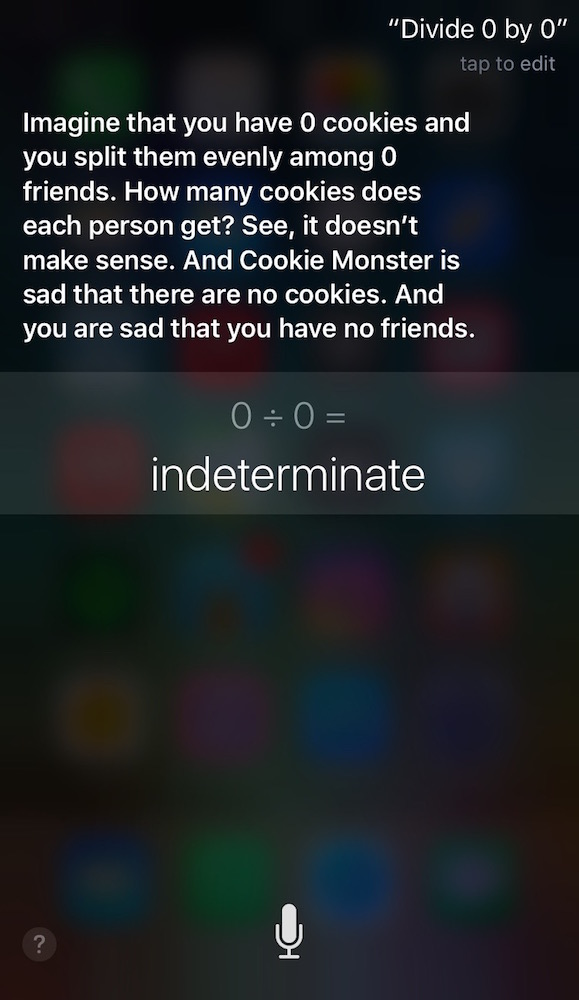
\includegraphics[width=.3\linewidth]{Graphics/3-2-Empirical-Cafe/ScreenshotSiri-Redacted}} \quad
    \subfloat[Google Now]
    {\label{fig:empirical cafe introduction screenshots googlenow}%
    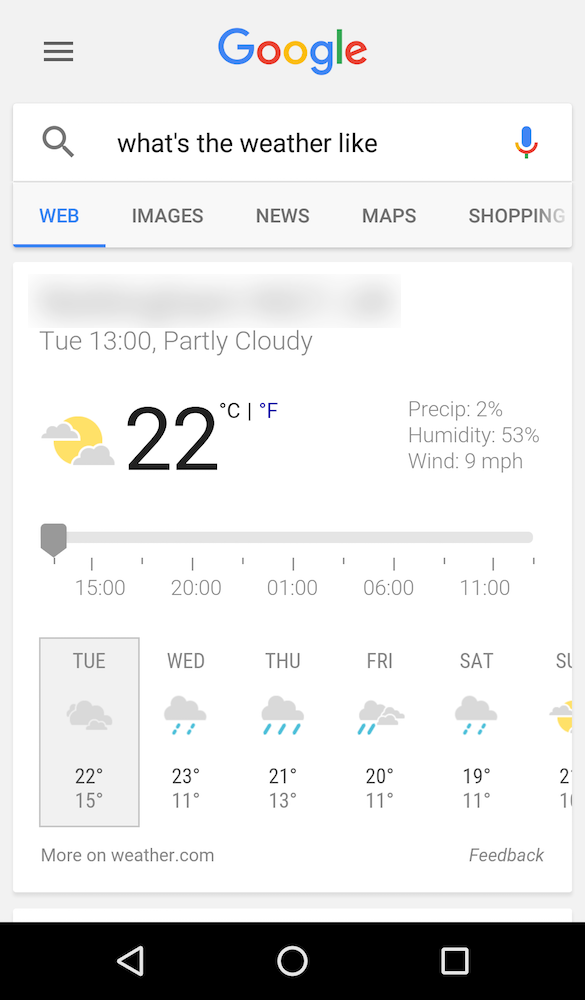
\includegraphics[width=.3\linewidth]{Graphics/3-2-Empirical-Cafe/ScreenshotGoogleNow-Redacted}} \quad
    \subfloat[Cortana]
    {\label{fig:empirical cafe introduction screenshots cortana}%
    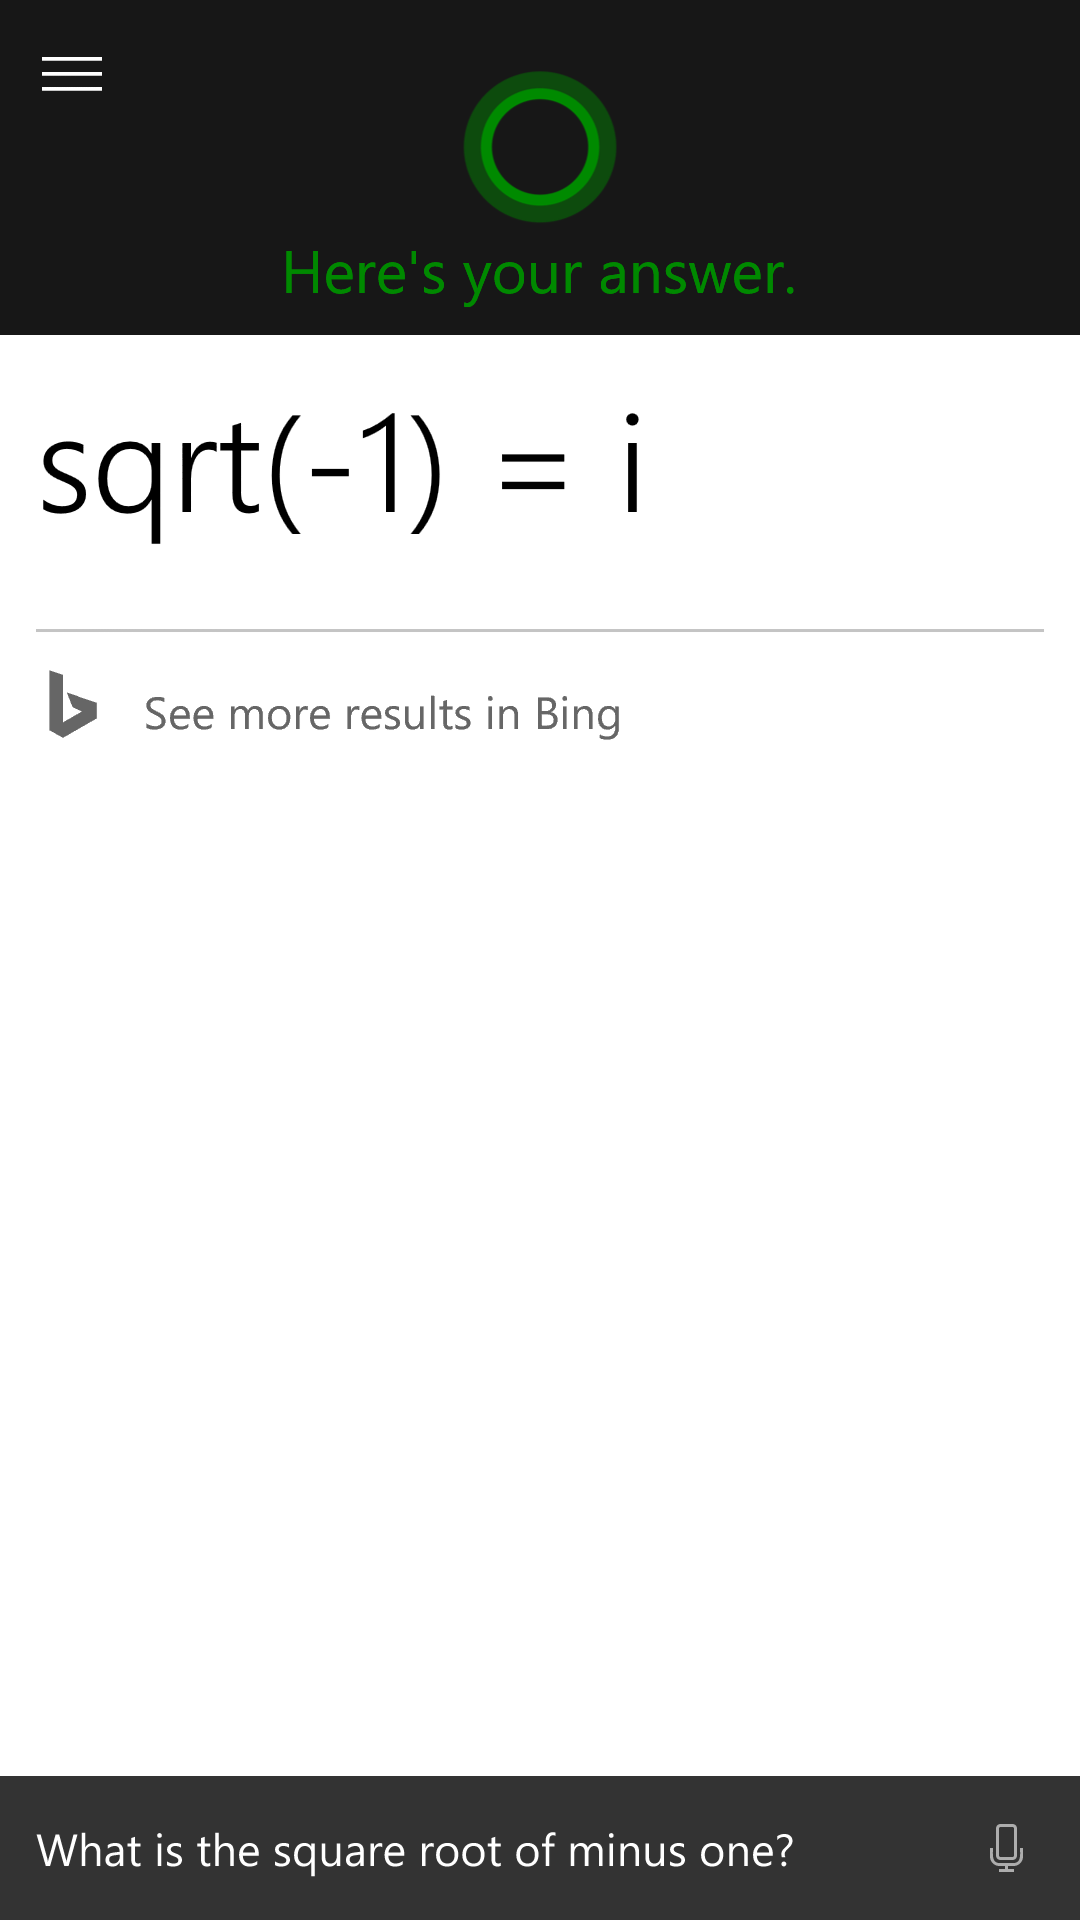
\includegraphics[width=.3\linewidth]{Graphics/3-2-Empirical-Cafe/ScreenshotCortana}}
    \caption[Example screenshots of different `Intelligent Personal Assistants' on commercially-available smartphones]{Example screenshots of different `Intelligent Personal Assistants' on commercially-available smartphones. The screenshots of Siri, Google Now, and Cortana are copyright Apple Inc., Google Inc., and Microsoft Corporation respectively. These screenshots were taken in 2016.}\label{fig:empirical cafe introduction screenshots}
\end{figure}

Early iterations of \acp{VUI} were focused on single tasks, such as \citet{Zue2000}'s JUPITER that was capable of providing weather information.
This particular system, as with others at the time, relied on people making telephone calls to interact with it, with the system engaging in dialogue with the interlocutor by talking back in a `conversational' manner.
As network connectivity and accuracy with automatic speech recognition improved, \acp{VUI}, such as InCa~\citep{Kadous2004}, were able to operate on portable mobile devices by making use of remote computing power and wireless communication technologies.
\acp{VUI} are now readily found on many devices such as smartphones, tablets, watches, and even televisions.
Additionally, although such systems fail to mimic human talk fully, \citet{Pelikan2016} were able to reveal the succinctness of how people adapt their talk to an assistant's needs and capabilities, making their interactions more successful.
Their work focused on a dyadic face-to-face conversation with a humanoid robot and was able to reveal a number of difficulties individuals face in such talk.
In this work, there is a pivot to considering how this talk unfolds as a situated action within a multi-party conversation.
A number of pieces of work focused on \acp{VUI} have suggested a number of positive aspects in order to justify their development further.
In one case, \citet{Jones2014} describe how a voice-controlled personal assistant could be used to support collaboration amongst those gathered around an interactive smart table, or for use in hands-free or `eyes-free' interaction while driving a car~\citep{Cycil2013}.
Others such as \citet{Luger2016}, however, paint a more challenging picture.
Through interviews, they found that there still exists a ``gulf between user expectation and experience''~\citep[p. 1]{Luger2016} with existing conversational agents and user expectations.
This gulf stems from people's perceptions that such systems should deliver more than they presently do and for issues with the \ac{VUI} communicating system functionality.
Innovations to address this gulf include features such as displaying understood text on a screen, voice typing~\citep{Kumar2012a} (i.e. live dictation), and the grounding (i.e. affirmation) of spoken input through responses~\citep{Clark1991,McTear2016}, although peoples' reported experiences suggest that numerous problems still remain.
By exploring the interactional accomplishment of using \acp{VUI} on smartphone devices \textit{in vivo} within a social gathering, and by employing a conversation analytic approach, a rich description of the collaborative work performed by members that occurs in, through, and around the \ac{VUI} use can thus be explicated.



% *********************************************************************************************************************



% \section{Research questions}\label{sec:empirical cafe rqs}
% The work in \autoref{ch:empirical pub} explored the collaborative practices that occurred within a social gathering in a pub while members made use of mobile devices through the touchscreen only, and in \ref{sec:empirical pub discussion coop} the practicalities of how members methodically collaborated in and through mobile device use was discussed.
% These primarily drew upon articulation work and accounting practices that members did to continue to display social engagement while embedding the device use within the social interaction.
% One potentially interactionally problematic feature of these sequences was the need for members to engage in accounting for device use because interacting with a (relatively) small personal device such as a smartphone precludes others from an awareness of device interaction that is unfolding.
% It was posited, and so is studied in this chapter, that speech interaction with a mobile device could free members from this practice as the production of talk is naturally accountable and so diminishes the necessity for members to methodically account for the use as a separate sequential act (see \ref{sec:empirical pub discussion problematic}).
% This chapter, then, sets out to unpack the work of using speech as part of the device interaction with the smartphone, and will continue to reveal the details of how interaction with the device is routinely embedded within conversation (RQ1), and how members engage in collaborative action in and through the interaction with the device (RQ2):
% \PrintRQ{1}
% \PrintRQ{2}



% *********************************************************************************************************************



\section{Study design}\label{sec:empirical cafe design}
 \begin{revisedsubmission}[JR-3a: Change EMCA to `study informed by EM']
A brief description of the setting in which the observations were undertaken is provided below, including details about the participants, and also the rationale for continuing to adopt an ethnomethodological and analytic orientation.
The study was approved by the university's School of Computer Science Research Ethics Committee.
\end{revisedsubmission}



% *********************************************************************************************************************



\subsection{The caf\'{e} as a study setting}\label{sec:empirical cafe design setting}
\begin{revisedsubmission}[JR-2b: Include details on the selection of the setting and the perspicuousness of the setting to the activity under study]
This chapter extends the work begun in the study of pub talk around touchscreen-based device use in the prior chapter by pivoting to exploring talk in a caf\'{e} around smartphone-based \ac{VUI} use.
In order to situate the study, a casual-social setting was chosen (see \ref{sec:empirical pub design setting}) to conduct a number of observations of friends socialising together.
As discussed, this study deviates from the prior examination of touchscreen-based device use by \textit{requesting} participants to use the voice-based personal assistant on their device instead of typing.
All participants were required to have used the assistant before the study.
It was supposed that given the identical premise of participant activity (i.e. of a gathering to socialise and relax), that the difference in setting would not be influential on the participants' use of devices (nevertheless, such a concern was not a primacy in this research given the analytic orientation, as discussed in the next section).

Although the particulars of activities that take place in a caf\'{e} may differ from that of a pub, to those who choose to gather there as a group of friends, the purposes remain the same: to socialise and relax together.
In other words, although the food may be different and there may be less sport or alcohol, the purposes for being in the setting as a group remain consistent.
Indeed, caf\'{e}s were also included within the definition of ``third places''~\citep{Oldenburg1989}, from which this thesis' more encompassing definition of a casual-social setting was formed.
Oldenburg defined third places as spaces that are outside the home or work environment that support gathering, socialising, and relaxation for groups and individuals, and with this definition, a caf\'{e} is the epitome of a such a setting.
Work that has studied interaction in caf\'{e}s remarks upon how they provide a ``common code of conduct''~\citep[p. 210]{Laurier2001}  that is both informal yet still provides a guidance of behaviour that is adhered to by members, but typically lack ``complex articulation and coordination work'' found in more formal settings~\citep[p. 222]{Laurier2001}.
Laurier, a number of years later, in studying interactions in a caf\'{e}, introduces caf\'{e}s in the UK and USA as ``familiar nodes in the network of gathering places that remain a necessity for the accidental tourists, be they business executives, chefs or mathematicians, who shuttle back and forth stitching regions together''~\citep[p. 5]{Laurier2008a}.
It is through this text that the significance of caf\'{e}s is realised as spaces in which different people in different situations gather for various purposes.
Indeed, during the observations that took place for the work in this thesis, the caf\'{e} received a constant stream of visitors, some merely taking drinks to go, and some meeting up with others, some brought children and some arrived as groups of friends.
Therefore, such a setting is perspicuous to observe a gathering of friends socialising.
\end{revisedsubmission}



% *********************************************************************************************************************



\subsection{Collecting data in the caf\'{e}}\label{sec:empirical cafe design participants}
In the study, a neighbourhood caf\'{e} was selected that served hot and cold food, cakes, and drinks.
The caf\'{e} is in a residential suburb of Nottingham, within a pavilion at a local park and nearby to schools and a university.
Suitable times for observations were agreed between the caf\'{e} and participants, allowing for video and audio recording of the friends talking during a gathering lasting up to ninety minutes.
All sessions were recorded on weekday afternoons when the caf\'{e} was open to the public.
\iresubmission*[ER-F, ER-G1: Specify how data were collected in practice]{Video capture was completed by two fixed wide-angle cameras on tripods with an audio recorder placed on the table to allow for clearer capture of talk between the participants.}

Groups of friends were recruited via email and social media to visit the caf\'{e} together for the purposes of socialising.
Prior to the study, participants were asked whether they had previously used a personal assistant on their mobile device, although there was no frequency or expertise required by them in order to take part.
Three groups of four friends were recruited to go to the caf\'{e} together over a two-month period.
Seven participants self-identified as male, and five as female; they ranged in aged from 22 to 37. % (M = 28.75).
All participants gave informed consent and were reimbursed for their time with a shopping voucher.
During the studies, all participants drank various drinks, some ate cake, and one brought some light reading with them to do as they were chatting with their friends.



% *********************************************************************************************************************


%\subsection{Methodology}\label{sec:empirical cafe design methodology}
The study approach is most aptly described as participant-observer, with a researcher present at the table conversing with the group where relevant.
The group of friends met the researcher at the caf\'{e} and were asked to complete a consent form prior to data capture.
They were free to move about in the caf\'{e} although primarily sat around a single table as they socialised, drank, and ate cake with each other.
For the study, participants were asked to preferably use the personal assistant on their mobile devices instead of typing where possible\footnote{The information sheet provided to participants prior to the study is included in \appref{app:studyinfo-cafe infoconsent}} adjusting the study to be as close to `natural' as feasibly possible to that of a study of interactions that are somewhat prescribed by very nature of the enquiry.
However, the methodological approach to studying interaction remains steadfast given the analytic orientation to the accomplishment of members in and through interaction, irrespective of \textit{reasons why}.

As per \autoref{ch:empirical pub}, there was no requirement to use a device, and there were no tasks set for the friends to perform during the study.
The idea of curating a number of tasks for groups to perform with \acp{VUI} during the sessions was considered, however following a pilot study in which participants were given `free reign' on what activities to perform during the study, and told to converse as they normally would, it was concluded that this was not needed–--people still chose to use the \acp{VUI} on their devices.
Therefore, participants were simply asked that they socialise and when the opportunity arose, they use a \ac{VUI} instead of typing, if appropriate.
After the study, a number of informal questions to gauge feedback and gather personal perspectives on the use of \acp{VUI} were asked.
However, this group interview was used as a debriefing exercise rather than to shape the findings.



% *********************************************************************************************************************



\subsection{Analysing the collected data}\label{sec:empirical cafe design analysis}
\begin{revisedsubmission}[ER-G1: Add further information about the analysis of the corpus, primarily the selection of fragments]
To analyse the collected corpus, as with the prior study, an analysis shaped by ethnomethodology~\citep{Garfinkel1967, Sacks1974} was performed.
Through this, the orderly and situated practice of using \acp{VUI} in conversation was explicated.
This analysis required the watching of the collected corpus multiple times, in order to segment and identify relevant fragments of data consisting of \ac{VUI} use.
Firstly, fragments were watched (and re-watched), with the methodical actions of members within the setting catalogued and indexed to identify instances where a mobile device and a \ac{VUI} was used.
Timestamps and descriptive language were used to construct a record of the interactions that took place, which allowed for iterative re-examining of prior data with relative ease to help gain an overall impression of the data collected across all the sessions.

Three fragments were selected for presentation in this chapter.
In line with best practice, as summarised by \citet{Heath2010}, each fragment progressively reveals the organisation of interaction with and around the use of the device:
\begin{quote}
    As you build an argument the analysis should be progressively revealed and emerge by virtue of the presentation of each successive extract. Furthermore the fragments should become more delicate and complex such that the audience can learn how to see the phenomena and can follow the argument as it unfolds.
    \quoteauthor{\citet[p. 111]{Heath2010}}
\end{quote}
In the three fragments to be presented, the first illustrates a typical use of a \ac{VUI} on a smartphone to introduce new information to the conversation that will set the scene for the interactions that unfold.
The second fragment introduces a more complex case that reveals how users perform additional actions to get the \ac{VUI} to work as desired.
The final fragment introduces an interactionally problematic case where a member uses the \ac{VUI} to establish its capability, revealing the richness and complexity of interaction around the use of a \ac{VUI} in a caf\'{e}.

The work was oriented to unpacking the retrospective-prospective character (see \ref{sec:background approach em sequentiality}, \citet[pp. 35--75]{Garfinkel1967}) of members accomplishing the work of using a \ac{VUI} in this setting, in and through their ongoing social interaction.
This orientation necessitated the identification of interactional accomplishments that occasioned the use of the \ac{VUI}.
This included how the device was introduced, the instruction or question that formed the request to the \ac{VUI}, the actions (in-talk and physical movements) of members in the setting throughout the activity, and so on.
In other words, this orientation, and the resulting analysis, allowed for the formation of a comprehensive understanding of the activities performed by members in using the \ac{VUI}.%, as per RQ1.
%In turn, the collaborative efforts undertaken by members in the setting were revealed through the sequences of contingent and contextually shaped action, as per RQ2.
\end{revisedsubmission}

In total, 40 episodes of \ac{VUI} use in the sessions were identified (some of which were overlapping), with episodes ranging from a few seconds to a nearly five minutes in length.
\iresubmission*[ER-G1: Add further information about the analysis of the corpus, primarily the selection of fragments]{A substantive review of the episodes was performed to examine the interaction that unfolded, honing in on episodes that represented observable-reportable intersections of the use of the \ac{VUI} and conversation for a more in-depth analysis.
Six fragments were then transcribed with both verbal (i.e. talk) and non-verbal actions (e.g. gestures and other interactional resources) being carefully noted.
These fragments were selected in line with the aims of this research to reveal the social organisation of device use in the use of \acp{VUI} in and through conversation and that were deemed to warrant further investigation.%, with each fragment being reviewed individually and discussed collaboratively with other researchers multiple times.
}



% *********************************************************************************************************************



\section{Findings}\label{sec:empirical cafe findings}
\begin{revisedsubmission}[JR-3a, JR-3c: New structure and framing of the analysis]
Data from the fieldwork will now be introduced and presented over a series of `data excerpts'---these excerpts form fragments that \textit{vividly exhibit}~\citep{Crabtree2012} the actions of members within the collected corpus.
Each of these fragments exhibits the activities of members' observed practices of how members made use of the \acp{VUI} on their personal devices in the caf\'{e}.
% The first fragment provides a preliminary sense of what interaction with a \ac{VUI} \textit{looks like}, revealing how devices can be used to retrieve new information for conversation (c.f. \ref{sec:empirical pub findings newinfo}).
% The second fragment introduces a more complex ample of how members answer questions in conversation using the device, and how collaborative efforts ensure in getting a device to work.
% The third fragment introduces interaction that unfolds as a result of the design of \acp{VUI}---using the \ac{VUI} to establish its capability.
% Throughout the explication of the fragments, the practice of how device use is used as a mundane activity in ``caf\'{e
% } talk'' will be established.
\end{revisedsubmission}

%By orienting to the sequentiality of using \acp{VUI} on a portable device in conversation, the nature of how the members' actions were occasioned in and through interaction, and, sequentially, what this methodical and situated practice brought about are explicated.
%Vivid exhibits~\citep[p. 112]{Crabtree2012, Bannon1993} of the accomplishment of using \acp{VUI} are provided to exemplify the orderly practice of members and present a rich picture of how members' use of their mobile devices unfolds.
In total, the corpus consists of 123 utterances to \acp{VUI} by members, across 40 distinct episodes of data from a corpus consisting of 3.6 hours of video data.
In particular, this chapter will reveal (1) how members perform a request with their device, (2) how members orient to and appropriately deal with the request and the \ac{VUI}'s response to the request, and (3) how members collaborate through the interaction with the \ac{VUI}. 

\appref{app:notation} provides details of the transcript notation used in this thesis.
All names and identifiable information within the transcripts provided are entirely fictional.

\begin{revisedsubmission}[JR-3a, JR-3c: Introduce the new fragments structuring]
%ata from three distinct fragments are now presented with the following corresponding findings: the first fragment  revolves around where a member of the setting uses the \ac{VUI} to \textit{introduce new information for conversation} (akin to what was identified previously in \ref{sec:empirical pub findings newinfo}, see \ref{sec:empirical cafe findings newinfo}),  the second focuses further on people using a \ac{VUI} to answer a question to verify information in conversation (see \ref{sec:empirical cafe findings answering}), and the final fragment introduces a situation in which individuals work to identify and confirm the capability of a \ac{VUI} (see \ref{sec:empirical cafe findings capability}).

% In the following fragments, The use of a \ac{VUI} will be shown to consist of two key instrumental activities across all fragments of data in this chapter:
% \begin{itemize}
%     \item Preparing and addressing the \ac{VUI}, and
%     \item Responding to the \ac{VUI}
% \end{itemize}
\end{revisedsubmission}



% *********************************************************************************************************************



\subsection{Introducing new information for conversation}\label{sec:empirical cafe findings newinfo}
\begin{revisedsubmission}[JR-3a, JR-3c: This section is new, reconstructed from prior analysis]
The first fragment, called \textit{When Does the Sun Go Down?}\footnote{The complete fragment is included in \appref{app:fragments-cafe sunset}.}, that commences in \autoref{frag:empirical cafe findings newinfo-i}, consists of four friends: Arthur, Harry, Sally, Julia, and the researcher.
The friends are meeting late afternoon during winter and the sun is shining into Harry's eyes.
He holds his hands in front of his eyes although he refuses to move because he will \QF[01]{...be fine in like three minutes}.
The friends joke about this experience, and that this forms part of their study (lines 08–15), but this challenge of the blinding sunlight establishes the interactional project that ensues.
Later in the next excerpt, Julia uses her iPad, which she had out on the table already, to find the time of sunset as a result.

\begin{inlinefrag}
    {\fragresubmission{JR-3c, ER-H: Revised fragment that is shorter, with labels on the image for the speakers}
    \begin{transcript}
        \by HAR {i’ll be fine in like three minutes ((holds hands in front of} \\
        \by     {eyes))} \\
        \by RES {keeps coming back as well like} \\
        \by SAL {as soon as you cha\emph{nge} it comes back} \\
        \by JUL {yeah yeaha} \\
        \later  {0.3} \\
        \by RES {there’s actually just someone out there with a light!} \\
        \by ALL {((laugh))} \\
    \end{transcript}
    \caption{When Does the Sun Go Down? (i)}\label{frag:empirical cafe findings newinfo-i}
    \begin{figure}[bth]
        \centering
            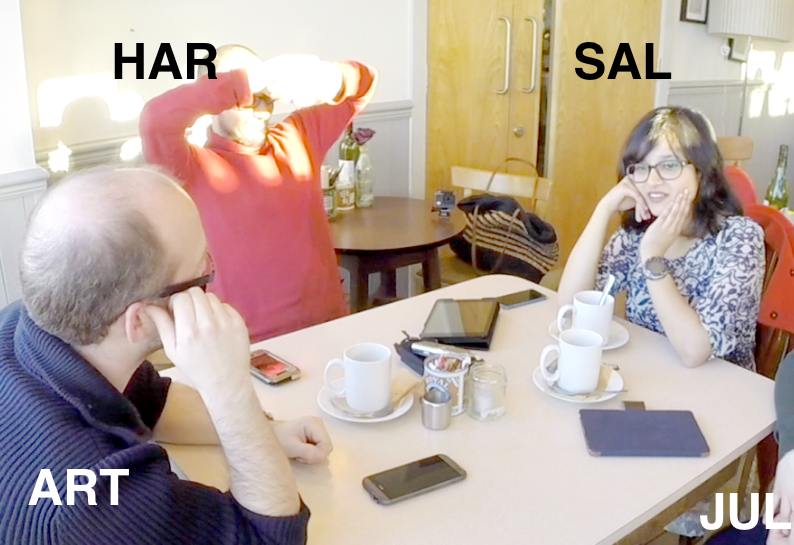
\includegraphics[width=.7\linewidth]{Graphics/3-2-Empirical-Cafe/FragmentSunset-1}%
        \caption{HAR blocks the sunlight in his eyes (\autoref{frag:empirical cafe findings newinfo-i}: When Does the Sun Go Down? (i), line 1)}\label{fig:empirical cafe findings newinfo-i}
    \end{figure}
    }
\end{inlinefrag}

In this opening excerpt, the group jokes about the sun shining through a nearby window into Harry's eyes as a result of the time of day (approximately evening time, around sunset).
This occasions, as will become evident in the following excerpts, Julia to use her \ac{VUI} to retrieve the time of \textit{sunset} for this given location.
This work to establish the time of sunset addresses the ongoing concern established in conversation about the sun in Harry's eyes, and responds to his remark that he will \QF[01]{be fine in like three minutes}, with the use of the \ac{VUI} commenced by Julia to introduce new information to \textit{verify} his claim. The next two sections, centred around two excerpts that follow Julia as she seeks new information for the conversation:
\begin{enumerate}[label=(\roman*)]
    \item \nameref{sec:empirical cafe findings newinfo addressing}, and
    \item \nameref{sec:empirical cafe findings newinfo collab}.
\end{enumerate}

As will be evident through the sequential revelation of members' actions, the \ac{VUI} will be introduced and used with the address of a question occasioned in and through the conversation.
The nature of multi-party conversation and making a device interaction accountable will allow members to engage with the interaction at hand in the completion of one member's interactional project to verify the time of sunset.
\end{revisedsubmission}



% *********************************************************************************************************************



\crpagebreak\subsubsection{Addressing the question to the VUI}\label{sec:empirical cafe findings newinfo addressing}
\begin{revisedsubmission}
The discussion continues before the next excerpt, \autoref{frag:empirical cafe findings newinfo-ii}, picks up the conversation.%, with the members of the group joking that the light in Harry's eyes is a result of someone standing outside the window with a torch, or as a result of the study itself.

\begin{inlinefrag}
    {\fragresubmission{JR-3c, ER-H: Revised fragment that is shorter, with labels on the image for the speakers}
    \begin{transcript}[16]
        \by JUL {[ ((removes cover from device but leaves open)) ]} \\
        \by SAL {((laughs))} \\
        \by JUL {((presses button on device))} \\
        \by HAR {there we go!} \\
        \by JUL {\textbf{what’s the time of sunset?}} \\
        \later  {1.3} \\
        \by ALL {((gaze at the tablet))} \\
        \later  {3.0} \\
        \by JUL {ok! \textit{// ((device displays clock)) //}} \\
        \by ART {((leans in to look))} \\
        \by SAL {that’s [ a~~~~~~] fucking analogue clock it pisses me off!} \\
        \by HAR {~~~~~~~[ today? ]} \\
        \by HAR {ilunno (0.6) 24 hour=} \\
        \by JUL {<no no no!> it misunderstood actually (0.8) understood what’s the} \\
        \by     {~[ time ]} \\
        \by HAR {~[ time ] now} \\
    \end{transcript}
    \caption{When Does the Sun Go Down? (ii)}\label{frag:empirical cafe findings newinfo-ii}
    \begin{figure}[bth]
        \centering
            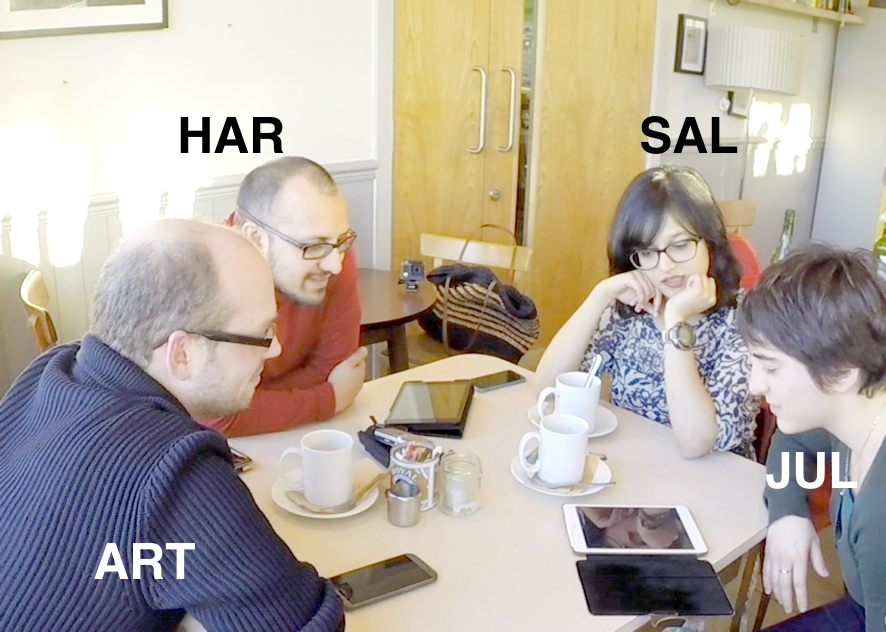
\includegraphics[width=.7\linewidth]{Graphics/3-2-Empirical-Cafe/FragmentSunset-2}%
        \caption{All members gaze at the tablet (\autoref{frag:empirical cafe findings newinfo-ii}: When Does the Sun Go Down? (ii), line 25)}\label{fig:empirical cafe findings newinfo-ii}
    \end{figure}
    }
\end{inlinefrag}

First, this excerpt is unpacked.
As the laughter begins to die down within the group at the start of the excerpt, Julia removes the cover from her device, which she has on the table (line 16); she waits for the group laughter to die down, presses the home button (line 18), and begins her utterance as Harry finishes remarking that the sun has now moved (line 19).
Julia uses her device's \ac{VUI} to ask for \QF[19]{the time of sunset}.
As she does this, she fixes her gaze at the screen, which displays a loading animation while the device is awaiting input.
At this point, all members lean in towards the device, as shown in the image, and demonstrate an awareness of an impending response from the \ac{VUI}.
As she began her request, Harry utters \QF[18]{there we go} in direct response to the sun no longer coming through the window directly into his eyes (inferred by his shift in posture, including no longer covering his eyes with his hands).
Nevertheless, Julia pressed ahead with the question, having begun the performance of preparing the device for the address by pressing the button.

After a few moments, the \ac{VUI} returns the time for the local area as an analogue clock.
A number of comments on this are passed: Sally comments on the presentation of the time (line 26) and Harry questions if that is for the present day (line 27).
Julia then interrupts the talk and retorts that she has realised the device has \QF[29]{misunderstood actually} and that the \ac{VUI} is presenting the current time, not the time of sunset.

By explicating the distinct sequential actions taken by members as the device is used, the ways in which members practically reason about how a \ac{VUI} responds to a request and attend to the \ac{VUI}'s response become evident (e.g. by leaning in, rotating gaze, not over-talking the \ac{VUI} or \ac{VUI}-user).
In this exhibit, Julia reasons about the failed outcome of the request to the \ac{VUI} through examining the displayed response, and makes this accountable to all (line 25) through her verbal report.
Her position and access to the device affords her greater visibility (as seen in the image in \autoref{fig:empirical cafe findings newinfo-ii}) of the response from the device, which typically displays the `transcribed' text of what the device `understood'.
Through her vocalised interpretation of the output of the \ac{VUI}, she provides an explanation for the problem source---or rather, starts to---as she realises it \QF[29]{understood what's the---} and Harry, who seemed to question the answer (line 27) completes her sentence with \QF[31]{time now}.
Harry's completion of Julia's utterance exemplifies that he is in accord with her reported interpretation of the source of technical trouble.

Through the ongoing interaction, as will be revealed in the next excerpt, members collaboratively reason that the response was not as expected and that this must be because the transcription of the request by the \ac{VUI} was wrong.
\end{revisedsubmission}



% *********************************************************************************************************************



\subsubsection{Collaboratively finding new information}\label{sec:empirical cafe findings newinfo collab}
\begin{revisedsubmission}
Julia's previous assessment that the device was showing the current time, as opposed to the time of sunset, (lines 30---32)  leads to a proposal to ask a different question (line 36) to the device from Julia.
In turn, the members collaboratively find words to return a successful result, as examined in this next excerpt, with Julia proposing a follow-up question, and Harry providing a suggestion of the wording she should use (line 35).

\begin{inlinefrag}
    {\fragresubmission{JR-3c, ER-H: Revised fragment that is shorter, with labels on the image for the speakers}
    \begin{transcript}[32]
        \by JUL {so-} \\
        \by ART {soaoah yeah\intUp} \\
        \by JUL {shall i ask (1.6) um:=} \\
        \by HAR {~~~~~~~~~~~~~~~~~~~~~=what time will the [ sun set? ]} \\
        \by JUL {~~~~~~~~~~~~~~~~~~~~~~~~~~~~~~~~~~~~~~~~~[ ((holds button)) ]} \\
        \by JUL {\textit{// ((audible chime)) //}} \\
        \later  {4.0} \\
        \by JUL {\textit{ // ((on screen text: go ahead i’m listening\ldots)) //}} \\
        \later  {0.3} \\
        \by JUL {\textbf{when does the sun go down?}} \\
        \later  {2.9} \\
        \by JUL {sunset will be at [ seventeen thirty two ]} \\
        \by ART {~~~~~~~~~~~~~~~~~~[ ther:::e you go~~~~~~]} \\
    \end{transcript}
    \caption{When Does the Sun Go Down? (iii)}\label{frag:empirical cafe findings newinfo-iii}
    % \begin{figure}[bth]
    %     \centering
    %     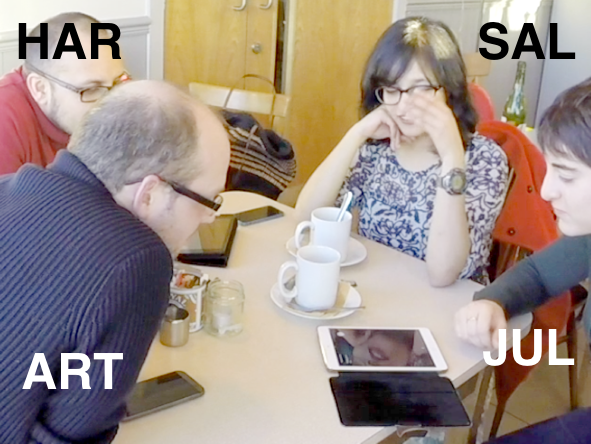
\includegraphics[width=.7\linewidth]{Graphics/3-2-Empirical-Cafe/FragmentSunset-3}%
    %     \label{fig:empirical cafe findings newinfo three}
    %     \caption{Members inspect the outcome of the request (\autoref{frag:empirical cafe findings newinfo-iii}: When Does the Sun Go Down? (iii), line 22)}\label{fig:empirical cafe findings newinfo-iii}
    % \end{figure}
    }
\end{inlinefrag}

In this final excerpt, Harry proposes a slightly different question (line 35) although ultimately Julia asks \QF[41]{when does the sun go down?}, to which the \ac{VUI} provides an accepted answer as revealed in Arthur's comment of \QF[44]{there you go}.
Although the time is visible on the screen and all members look at it, Julia also provides an audible report of the time displayed (emblematic of the \textit{hybrid} nature of \ac{VUI} interaction on a smartphone also making use of the screen).
This excerpt reveals how members can collaborate on a project by working together to use a device, exemplified in this fragment through the demonstrable reasoning of suggesting the cause of trouble and through reformulating the request by the members.
In the fragment, across the three excerpts, Julia interprets the initial result from the \ac{VUI} as incorrect (line 29), but then reasons about the response, reveals her reasoning to the group, and then asks the \ac{VUI} the same question with a different lexical construction (line 41).
In this, she does not just retry or repeat the same request, however, she rephrases---with the presumed aim of soliciting a successful answer from the \ac{VUI}, as per the occasioned purpose of her actions.

%Refinement can be seen as a subset of repeating, where a member may still seek to identify the same information but with a new request in order to retrieve a satisfactory result.
%Rephrasing was a common practice by members to attend to troubles with \acp{VUI} responding incorrectly; a total of 22 requests (out of 123) were posed to \acp{VUI} where lexically they were different, but the subsequent requests were reformulations of the same request\footnote{The initial analysis of the data and organised corpus included all the requests made to the devices and corresponding timestamps}.
Rephrasing a request, as occurred here, was a practice used by members to attend to and deal with troubles with \acp{VUI} responding incorrectly.
While in this case, the original interlocutor rephrased the request, on other occasions members other than the original \ac{VUI}-user may also have performed a rephrased version of the original request on their own device.
Therefore, it is posited that there is a distinction in the occasioning of rephrased requests and repeated requests.
Rephrasing occurs as members attend to a \ac{VUI} not completing their request as a result of the \ac{VUI} not completing a transcribed request as expected, e.g. as Julia informs others in the setting (line 29).
% Repetitions, on the other hand, are performed in response to members perceiving the \ac{VUI} to have mistranscribed the request (e.g. members speak slower, louder or more accentuated, but with the same word construction).
Given members' use of \acp{VUI} is for a specific purpose, members undertake and extend their occasioned activity of using the \ac{VUI} until receiving a response that accomplishes their goal.%\footnote{Such an outcome is not necessarily getting the `desired answer' but a response from the \ac{VUI} with which the user no longer continues interaction with a \ac{VUI} as a result of it.}.

Finally, this fragment concludes by remarking upon the collaborative and coordinated activity that occurs throughout this fragment.
The members collectively shift their body posture so that they are looking towards the device being used by rotating their torsos and leaning across the table.
Additionally, they mutually pause their talk while requests are performed and responses computed, they gaze at the tablet, and they attend to the answer as soon as it is provided---i.e. they work together to complete the request.
In this entire sequence, the request is interactionally occasioned in and through the conversation about the sun shining into Harry's eyes.
The other members then witness the request being performed (line 20), and the failure of the device to respond appropriately is made accountable by making the screen clearly visible to all members, such that the other members can see and practically reason about the result.
This, in turn, allows for members to collaboratively reason about the grounds of the \ac{VUI}'s failure (lines 29--35).
In attending to the failure, the members then construct a further request which leads to a satisfactory result.
Given that members accomplish the natural accountability of performing a request with a \ac{VUI} through conversation, it appears that the practice of rephrasing a request lends itself as a resource to support collaborative activity amongst the co-present members.

In this fragment, a device was brought into the conversation in order to introduce new information to the group in relation to a problem established through interaction.
Although the \ac{VUI} user encountered \textit{technical} trouble, through suggestions from others, the member was able to complete their request and introduce the new information to the conversation.
Given the hybridity of interactions with \acp{VUI} on smartphones also featuring a \ac{GUI}, this introduction of information occurred through members looking at the information displayed on the screen of the device.
The next fragment moves beyond an example where new information is introduced into conversation to a situation where members are trying to answer a proposed question in talk.
At face value, this fragment seems to occur in the same manner as the first one, although through unpacking the data, interaction will be shown to be replete with challenges as members attend to problematic \ac{VUI} interaction.
\end{revisedsubmission}



% *********************************************************************************************************************



\crpagebreak\subsubsection{Methodical accomplishments in this fragment}\label{sec:empirical cafe findings newinfo methods}
\begin{revisedsubmission}
With this fragment, the work of introducing new information for conversation was unpacked over a series of excerpts.
The question was occasioned in and through the conversation, as a result of the sun shining into Harry's eyes, although Harry dismissed the problem as he expected the sun to set shortly.
Julia ostensibly uses this moment to ask the \ac{VUI} on her device the time that the sun will set, to determine the veracity of Harry's claim.
She does this by \textbf{preparing to use the \ac{VUI}} by removing the device's cover and holding the button down to activate the \ac{VUI}.
She then \textbf{addresses the \ac{VUI}} through talking to the device with her question and then \textbf{looks at the device} as it computes a response.
The co-present others also \textbf{lean in to look at the device screen} as an analogue clock is displayed, reasoning about the perceived incorrectness of what is displayed.
Harry and Julia \textbf{propose that the incorrect information} is displayed as a result of the device `misunderstanding' the request, and \textbf{propose a new wording}.
Julia \textbf{re-addresses the \ac{VUI}} through talking to the device again with a rephrased request, \textbf{looks at the device} along with the others as the response is computed, and then \textbf{provides a verbal report} once an answer is given.
This successfully completes the interactional project which was occasioned.
\end{revisedsubmission}



% *********************************************************************************************************************



\subsection{Answering a question in conversation}\label{sec:empirical cafe findings answering}
\begin{revisedsubmission}
The opening excerpt from the second fragment, titled \textit{Do Animals Have Accents?}\footnote{The complete fragment is included in \appref{app:fragments-cafe animals}.}, is given in \autoref{frag:empirical cafe findings answering-i}.
This excerpt unfolds as four friends: Lily, Gary, Karl, Antonius, and the researcher, are socialising together.
The group, which consists of members from the UK, Romania, and Austria, have been discussing the different onomatopoeic sounds that various animals make and how these sounds vary by country and language.

\begin{inlinefrag}
    {\fragresubmission{JR-3c: Revised fragment that is shorter}
    \begin{transcript}[5]
        \by KAR {do cats acth- (0.5) can you work out whether it's french because} \\
        \by     {because its talking in a- doing a french cat impression} \\
        %\im    1 {Graphics/3-2-Empirical-Cafe/FragmentAnimals-1.png}
        \by LIL {i::::: think some animals you can} \\
        \later {1.9} \\
        \by LIL {((picks up phone from table))} \\
    \end{transcript}
    \caption{Do Animals Have Accents? (i)}\label{frag:empirical cafe findings answering-i}
    }
\end{inlinefrag}

There are presently two conversation floors\footnote{In other words, within the group there are two discussions continuing in parallel with those co-present orienting to one conversation at a time~\citep{Edelsky1981}.} taking place in the conversation: in the floor focused on here, Karl asks Lily about animal accents before recounting scenes from a television show to Lily (omitted from this thesis for clarity), and in the other floor Antonius is recalling the sounds different animals make when uttered in Austrian German.
Just before Karl begins to recount his story, Lily picks up her smartphone (line 09) and begins to type with the on-screen keyboard throughout the story.
\iresubmission*[JR-3a, JR-3c: This section is new, reconstructed from prior analysis]{In the case of this fragment, the actions of members will be shown to consist:}
\begin{revisedsubmission}
\begin{enumerate}[label=(\roman*)]
    \item \nameref{sec:empirical cafe findings answering address},
    \item \nameref{sec:empirical cafe findings answering repeating}, and
    \item \nameref{sec:empirical cafe findings answering others}.
\end{enumerate}
\end{revisedsubmission}

These three activities are now unpacked below.
As will be evident through the sequential revelation of the action, members collaboratively work together to undertake action in their orientation to the problem that occasioned the use of the \ac{VUI}.
Given the nature of multi-party conversation, these activities will be shown to be recurrent and overlapping with each other, rather than discrete temporally-ordered accomplishments.
\end{revisedsubmission}



% *********************************************************************************************************************



\crpagebreak\subsubsection{Addressing the question to the VUI}\label{sec:empirical cafe findings answering address}
\begin{revisedsubmission}
After the story in which Karl recounts an episode of a television show, both he and Lily laugh and then he orients to and engages with the other floor; he does this by shifting his gaze to look at the others in the other conversational floor (specifically Antonius, who is talking at that moment)\footnote{In other words, Karl shifts his gaze and body posture away from the members he was previously conversing with the others at the table to those he was not conversing with, but who were conversing with each other in parallel.}.
At this point, Lily moves her smartphone closer to her mouth and asks her \ac{VUI} \QF[42]{do animals have accents?}.
This question was not specifically asked in talk but arises as a result of the topic that all the members have focused on in both floors at some point---in other words, the work of answering this question was occasioned in (and as a direct consequence of) the conversational topic.
Following Lily's request, a short gap in talk (line 43) unfolds before Gary shifts his gaze to Lily and responds to her question, as shown in the video still captured at line 44, even though her question was aimed at her \ac{VUI}.

\begin{inlinefrag}
    {\fragresubmission{JR-3c, ER-H: Revised fragment that is shorter, with labels on the image for the speakers}
    \begin{transcript}[40]
        \by LIL {er:::m: ((holding phone in front of her at chest level))} \\
        \later  {3.7} \\
        %\im    3 {Graphics/3-2-Empirical-Cafe/FragmentAnimals-2.png}
        \by LIL {((moves phone up to face)) \textbf{do animals have acce\emph{nts}?}} \\
        \later  {2.1} \\
        \by GAR {((shifts gaze to LIL))} \\
        \by     {yes they do actually! i think i've read something} \\
        \by LIL {i think i have [ too\intDown{}~~]} \\
        \by GAR {~~~~~~~~~~~~~~~[ yeas!~] [ (0.6) \emph{cows}! i- i~~~~~~~~~~~~~~~]} \\
        \by     {~~~~~~~~~~~~~~~~~~~~~~~~~read about cows that they have} \\
        \by     {~~~~~~~~~~~~~~~~~~~~~~~~~different accents around the world} \\
        \by KAR {~~~~~~~~~~~~~~~~~~~~~~~~~[ you missed mine- my racist joke ]} \\
    \end{transcript}
    \caption{Do Animals Have Accents? (ii)}\label{frag:empirical cafe findings answering-ii}
    \begin{figure}[bth]
        \centering
            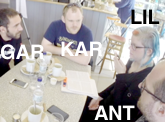
\includegraphics[width=.5\linewidth]{Graphics/3-2-Empirical-Cafe/FragmentAnimals-2}%
        \caption{Lily performs the request (\autoref{frag:empirical cafe findings answering-ii}: Do Animals Have Accents? (ii), line 44)}\label{fig:empirical cafe findings answering-ii}
    \end{figure}
    }
\end{inlinefrag}

In this second excerpt, Lily prepares to perform an utterance (line 40--42) and performs her utterance (line 42), first by moving the phone closer to her mouth with the handset held such that the microphone is in front of her lips, and then performing her utterance while there remains a gap in talk.
Following this utterance, Gary rotates his head from Antonius to Lily and responds to her question: \QF[43]{yes they do actually}.
Karl and the researcher also shift their gaze towards Lily, in the case of Karl by leaning back slightly and rotating his head, while the researcher rotates his head alone.
Through his response to Lily's question, Gary exemplifies the manner in which interactions with a \ac{VUI} are made accountable insomuch that others can observe, report upon, and respond to the device interaction accordingly---in this case, to answer the question Lily asked.
In this sense, this reveals how the preparatory action of talking to a \ac{VUI} on a personal device is made naturally accountable, and can be oriented to by co-present others as a matter occasioning further discussion.

Following this response by Gary to Lily's address to her \ac{VUI}, Lily affirms that she too had heard something\footnote{A story regarding cows with regional accents had been on the BBC News website a few days prior to this gathering.}.
In this, Lily implies that her question was guided by her being unsure (\QF{i think}, line 46), but occasioned by both the conversation and recent news events that she had read about; with Gary acknowledging he was aware of the story too (lines 46--49).
\end{revisedsubmission}



% *********************************************************************************************************************



\crpagebreak\subsubsection{Repeating a request to the VUI}\label{sec:empirical cafe findings answering repeating}
\begin{revisedsubmission}
Following this brief discussion between Lily and Gary following Lily's \ac{VUI} use, Lily has been looking at her device sporadically while talking to Gary.
She then lifts the device closer to her face again, and performs a new request to the device, which is indicated in the commencement on the next excerpt, \autoref{frag:empirical cafe findings answering-iii}.
In this next excerpt, the work of how members \textit{respond to the \ac{VUI}'s response} by repeating the request in order to accomplish their task is demonstrated. %, which, in this case, is of answering a question occasioned in conversation.

\begin{inlinefrag}
    {\fragresubmission{JR-3c: Revised fragment that is shorter}
    \begin{transcript}[51]
        \by LIL {\textbf{DO: \emph{ANIM}ALS HA\emph{V}E \emph{ACCEN}TS!}} \\
        \later  {2.4} \\
        \by LIL {°rubbish°=} \\
        \by KAR {~~~~~~~~~~~=parrots presumably do=} \\
    \end{transcript}
    \caption{Do Animals Have Accents? (iii)}\label{frag:empirical cafe findings answering-iii}
    }
\end{inlinefrag}

%This excerpt features multiple further addresses to a \ac{VUI}: first with Lily (line 51), then Lily and Karl (line 58), then the researcher (line 63), and then finally Lily (line 64).
This short excerpt features the first attempt at responding to the \ac{VUI}'s perceived failure to perform as expected, which in this case is done by repeating the request with greater volume and impetus (differing from the previous fragment in which a rephrased request was made, see \ref{sec:empirical cafe findings newinfo collab}).
As Lily does this, a gap in talk occurs (line 52) as other members look at Lily; she then quietly utters \QF[53]{rubbish}.
In and through this utterance she further accounts that the device has failed to adequately respond to the request put forward in her address to the device.
The repetition of the phrase, and increasing volume makes evident the device's failure to `hear' what is said.
Here, this demarcates a different problem with \acp{VUI}---not only do such devices have trouble responding correctly to what is said, at times they may not `hear' words at all.
\end{revisedsubmission}



% *********************************************************************************************************************



\subsubsection{Getting others to perform the request}\label{sec:empirical cafe findings answering others}
\begin{revisedsubmission}
The final excerpt from this fragment, given in \autoref{frag:empirical cafe findings answering-iv}, concludes Lily's efforts to find the answer to the question of whether animals have accents.
In this next excerpt, Lily asks Karl to help her complete the request, which she does by passing the responsibility of uttering the request to Karl by holding the device in front of Karl and questioning whether he could \QF[55, shown in \autoref{fig:empirical cafe findings answering-iv}]{ask it}.

\begin{inlinefrag}
    {\fragresubmission{JR-3c, ER-H: Revised fragment that is shorter, with labels on the image for the speakers}
    \begin{transcript}[55]
        \by LIL {~~~~~~~~~~~~~~~~~~~~~~~~~~~~~~~~~~=can you ask it?} \\
        \by     {((holds phone out in front of KAR's face))} \\
        %\im    1 {Graphics/3-2-Empirical-Cafe/FragmentAnimals-3.png}
        \by RES {((retrieves phone out of pocket))} \\
        \by KAR {\textbf{DO: ANI\emph{MALS} HAVE ACC::\emph{ENT}S!}} \\
        \later  {0.9} \\
        \by LIL {no:!} \\
        \by RES {\textit{//~sorry i'm-~//}} \\
        \by RES {((RES touches screen to stop utterance))} \\
        \by RES {\textbf{do animals have accents?}} \\
        \by LIL {\textbf{d\emph{o:} \emph{anim}als ha\emph{v}e a\emph{ccents}?}} \\
        \by RES {\textit{//~ok i've found this on the web~//} (sigh)} \\
        \by GAR {do [ they?~~]} \\
        \by LIL {~~~[ ah (.) ] it's working now!} \\
     %   \by RES {((touches top search result on device screen))} \\
    \end{transcript}
    \caption{Do Animals Have Accents? (iv)}\label{frag:empirical cafe findings answering-iv}
    \begin{figure}[bth]
        \centering
        % \renewcommand{\thesubfigure}{42}
        % \subfloat[Lily performs the request]
        %     {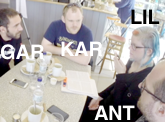
\includegraphics[width=.34\linewidth]{Graphics/3-2-Empirical-Cafe/FragmentAnimals-2}%
        %     \label{fig:empirical cafe findings answering two}} \quad
        % \renewcommand{\thesubfigure}{56}
        %\subfloat[Lily asks Karl to perform the request]
         %   {
            
\includegraphics[width=.7\linewidth]{Graphics/3-2-Empirical-Cafe/FragmentAnimals-3}
        %    \label{fig:empirical cafe findings answering three}}
        \caption{Lily asks Karl to perform the request (\autoref{frag:empirical cafe findings answering-iii}: Do Animals Have Accents? (iv), line 56)}\label{fig:empirical cafe findings answering-iv}
    \end{figure}
    }
\end{inlinefrag}

At the moment where Lily holds her device out to Karl and asks him to \QF[55]{ask it}, the researcher retrieves his phone from his pocket to perform the request (line 57).
Karl's request also fails, as revealed through Lily's next attempt (line 64), which this time yields search results, as does the researcher's (line 63).
Following the fragment, both begin to share information retrieved from webpages to the other members of the group.
This fragment is indicative of what \ac{VUI} use looks like–--that is, there are a number of grossly observable features that take place: there is ongoing selecting of speakers, repetition of requests, pauses in talk, body co-orientation and so on.

Importantly, one aspect revealed through close examination of the interaction is that once a request is performed with a \ac{VUI},  members' talk to \acp{VUI} may be sequentially followed by pauses in talk (lines 43, 52, 59), as members visibly orient their gaze towards a device as a response is computed.

% a number of practical actions are undertaken by members as they accommodate the utterance within the conversation.
% Talking to a \ac{VUI} is naturally accountable in addition to being occasioned in and through the social interaction of members in the setting.
% The accountability of action is premised on the fact that members of a setting can observe and report the action~\citep{Garfinkel1967}, and this is a feature of talk-in-interaction.
% Thus, talking to a \ac{VUI} immediately makes audible what is being undertaken to all within earshot.
% A member's device input is made directly accountable through talk, unlike interactions on touchscreens where the device user may have to provide explicit accounts to make the action accountable (as revealed in \autoref{ch:empirical pub}).
% 
% This fragment also provides interesting markers to consider what specifically follows talking to a \ac{VUI}; in particular, this transcript reveals that
The excerpts in this fragment reveal how, as a practice, talking to a \ac{VUI} in turn occasions the mutual production of silence by the co-present members as they re-orient to the use of the \ac{VUI}, and in turn focus on the device or the interlocutor.
Members do not pause their interaction or `sit in silence' however, their embodied actions of gaze and body co-orientation furnish others with how they are focusing their attention, as they turn to the device interaction.
In effect, performing a request brings about a lapse~\citep{Hoey2015} in the conversation: neither the member who was performing the request selects to talk next, nor does any other member.
\acp{VUI} function by assuming a pause-in-talk specifies the completion of a request, thus a pause by the interlocutor is necessary.
%However, as other members await a result, they do not self-select in commencing a turn.
Therefore, it is noted that the data reveals that the action of performing a request with a \ac{VUI} may prescribe a lapse in talk and the mutual production of silence.
This action is, by definition, intrinsically and demonstrably collaborative---members collectively and collaboratively socially construct silence in orientation to the utterance to the \ac{VUI}.

Furthermore, this fragment features numerous repeated requests to \acp{VUI}: Lily gets Karl to perform the request as a result of her device's repeated failure.
In the fragment, Lily uses her smartphone on multiple instances to perform the request \QF*[42, 51, 58, 63, 64]{do animals have accents?}, each time with more impetus in her voice.
With each repeated request, Lily accounts for the device's failure to appropriately respond to her initial request: either the device has mistranscribed, or it has not transcribed at all, and so another attempt is required to complete the task at hand.
Whereas in the prior fragment, members were shown to revise or \textit{rephrase} a request to get the \ac{VUI} to work, here we see another action of members to accomplish the task at hand with a \ac{VUI}: repeating the request in cases where it seems a \ac{VUI} has not `heard' the request.
Thus, a finding is that members address a problematic interaction with a \ac{VUI} through the further production of talk: \textit{they repeat their request}, and that others may assist in this completion.

% Specifically, this fragment exemplifies that members repeat requests if a request `goes wrong'; this may seem like an obvious fact but one which is worth stressing as in the corpus of observations, a total of 31 requests (25\%) were identical in lexical terms to a prior request, although lexicality is only half of the story.
% Consider in the fragment where Lily repeats her request multiple times (lines 51, 58, 64).
% Although identical in language, the production of talk differs in each one: in the first, she uses a general conversational tone; her utterance is consistent with the ongoing conversation.
% With her second performance, however, she performs the request louder and emphasises key sounds; to members within the setting, she demonstrates her frustration with the device – its failure to transcribe her words requires her to try again.
% Therefore, this analysis reveals that the failure of the device's \ac{VUI} to adequately respond to request occasions the necessity to repeat the request, possibly with greater impetus.

Finally, Lily's actions, of talking with greater impetus and volume, and then getting someone else to talk, account that for her, the perceived source of device trouble is that the device cannot transcribe her utterances because of her diction\footnote{Lily's reasoning of the trouble source is made visible as a common-sense understanding to other members of the setting, including Karl, through the second production of the request that is  produced louder and with greater impetus.}, which results in her involving Karl in the task of talking to the \ac{VUI} to complete the request.
Her practice of involving Karl in the request has the interactional outcome of recruitment to resolve the trouble at hand with the device interaction, a fundamentally collaborative mechanism of social organisation~\citep{Kendrick2016}\footnote{\citet{Kendrick2016} refer to recruitment not as single or class of social actions, but as an interactional outcome achieved through methodical practices such as requesting or offering assistance.}.
\end{revisedsubmission}



% *********************************************************************************************************************



\subsubsection{Methodical accomplishments in this fragment}\label{sec:empirical cafe findings answering methods}
\begin{revisedsubmission}
The second fragment in this chapter reveals the work of answering a question in conversation using a \ac{VUI}.
Lily \textbf{prepares to use her device} to answer the question Karl has asked, \textbf{lifting her phone to her mouth} and \textbf{addressing the \ac{VUI}} through talk.
The device ostensibly does not respond; therefore Lily \textbf{re-address the \ac{VUI} with a higher volume and impetus in her delivery but using the same question}.
The device again `fails' to respond; thus Lily \textbf{asks another co-present member, Karl, to perform the request}.
He then \textbf{addresses the \ac{VUI} with a loud speaking voice and different emphasis} compared to Lily, but with the exact same question---again there is no response from the device.
The researcher then \textbf{retrieves his phone} and \textbf{prepares his \ac{VUI} by holding the button down}.
He \textbf{addresses his \ac{VUI}} with the same question while \textbf{Lily also addresses} her \ac{VUI} again.
Both members then \textbf{verbally report that their devices have computed responses} and then go on to \textbf{discuss the findings}.
In this regard, the interactional project of using a \ac{VUI} to answer a question in conversation is completed.
\end{revisedsubmission}



% *********************************************************************************************************************



\subsection{Establishing the capability of a VUI}\label{sec:empirical cafe findings capability}
\begin{revisedsubmission}[JR-3a, JR-3c: This section is new, reconstructed from prior analysis]
The first fragment in this chapter identified how members of the setting introduce new information into a conversation by using a \ac{VUI} to retrieve the information.
The second further identified how members are able to direct specific questions raised in a conversation to a \ac{VUI}, to answer and address information deficits amongst those who are co-present.
This final fragment, which commences in \autoref{frag:empirical cafe findings capability-i} and is called \textit{Hey Siri! \ldots Call My Mother}\footnote{The complete fragment is included in \appref{app:fragments-cafe mama}.}, focuses on the researcher and Gary discussing the capability and features of the \ac{VUI} on his device, again using the \ac{VUI} to address an information deficit.
However, whereas the first two fragments identify how members are able to use a \ac{VUI} in conversation to address problems established in and through conversation, this fragment deviates from this and reveals how \ac{VUI} use may be occasioned self-referentially in order to address matters of \ac{VUI} capability\footnote{This thesis strays away from attributing a reason beyond what is naturally accountable, but the recentness with which \acp{VUI} became available at the time of this study would suggest that there is not the same level of familiarity with their capabilities as with basic smartphone interactions completed using the \ac{GUI}.}.
First, this fragment will be introduced, with the problem at hand established, and then the fragment will be unpacked as two distinct activities, in which members undertake:
\begin{enumerate}[label=(\roman*)]
    \item \nameref{sec:empirical cafe findings capability establish}, and
    \item \nameref{sec:empirical cafe findings capability testing}.
\end{enumerate}

These two activities are now unpacked in the following sections to reveal the problem case of whether the device is able to deal with a similar but non-English spelling of contact details.
\end{revisedsubmission}



% *********************************************************************************************************************



\subsubsection{Establishing the desired function}\label{sec:empirical cafe findings capability establish}
\begin{revisedsubmission}[JR-3a, JR-3c: This section is new, reconstructed from prior analysis]
The premise of the problem established through the conversation between the pair is whether the device's \ac{VUI} is capable of matching the non-English spelling of `mama' in Gary's smartphone's address book, with the discussion predicated around the focus of the study.
The conversation commences in \autoref{frag:empirical cafe findings capability-i}, in a separate floor consisting of just Gary and the researcher, who are both sitting next to each other.
The other members of the setting are conversing while the two discuss Gary's interactions with his device.

\begin{fragfloat*}
    {\fragresubmission{JR-3c, ER-H: Revised fragment that is shorter, with labels on the image for the speakers}
    \begin{transcript*}
        \by GAR {i'm curious if I say in} \\
        \by     {romanian (.) to call my mother} \\
        \later {0.7} \\
        \by GAR {it will actually find the } \\
        \by     {contact for my mother is (.)} \\
        \by     {mama in romanian (.) } \\ %if I say} \\
        \later {\ldots}[5] \\
        % \by     {call my mum will it actually} \\
        % \by     {call my mother which is in a} \\
        % \by     {contact as mama (0.7) will it} \\
        % \by     {make the connection between} \\
        % \by     {mama and mum} \\
        \by RES {cos you can also tell people} \\
        \by     {who they (.) like you can say} \\
        \by     {like} \\
        \im 1   {Graphics/3-2-Empirical-Cafe/FragmentMamma-1.png}
        \by GAR {\textbf{hey siri=}} \\
        \by RES {~~~~~~~~~=my mother is this} \\
        \by     {~~~~~~~~~~person (0.8)} \\ \vspace{3.9cm}
    \end{transcript*}
    \nopagebreak[4]
    \caption{Hey Siri! \ldots Call My Mother, part (i)}\label{frag:empirical cafe findings capability-i}
    }
\end{fragfloat*}

As this exhibit commences, Gary questions, by way of asking the researcher indirectly, whether if he asks his device to call his mother, the device will recognise the name in his contact list (the contact's name is spelt `mama' in Romanian).
The researcher responds in broken English, alluding to a feature with \acp{VUI} and smartphones that allow for pseudonyms to be allocated to contacts, although his utterance is punctuated by Gary's initial commencement of device use, using the hotword \QF[15]{hey siri}.
Without shifting his gaze from the researcher who is speaking, Gary lifts his phone and performs this phrase and then moves the device back to chest height between him and the researcher, interleaving the opening utterance of the hotword within their conversation.

Gary's initial proposition (lines 01---06) establishes that he is curious about the capability of the \ac{VUI} and its ability to function as desired.
This is followed by the researcher discussing a feature that would potentially allow Gary to request a device to call his mother, using an alternative name to the name given to the contact in his phone's address book (lines 12---14).
As such, the researcher does not directly respond to Gary's question, but makes a proposition of a technical solution to the problem at hand, by adding an English pseudonym to the contact.
\end{revisedsubmission}



% *********************************************************************************************************************



\subsubsection{Testing the functionality by addressing the VUI}\label{sec:empirical cafe findings capability testing}
\begin{revisedsubmission}
Following the continuation of the researcher's utterance regarding the pseudonym functionality (lines 16---17), Gary glances at his device and re-performs the hotword to activate his \ac{VUI}.
This next exhibit, \autoref{frag:empirical cafe findings capability-ii}, reveals how Gary tests the functionality of the \ac{VUI} with his desired capability, which allows him to demonstrate, either successfully or not, his suspicions of a limitation of the device to deal with alternative spellings of words such as \textit{mamma}.

\begin{inlinefrag}
    {\fragresubmission{JR-3c, ER-H: Revised fragment that is shorter, with labels on the image for the speakers}
    \begin{transcript*}[18]
        \by GAR {((glances down at screen))} \\
        \by     {((moves device in front of} \\
        \by     {mouth)) \textbf{hey siri}} \\
        \by GAR {((moves device to chest} \\
        \by     {height between the two))} \\
        \later  {1.0} \\
        \by RES {i'd press the button} \\
        \later  {1.2} \\
        \by GAR {((moves device in front of} \\
        \by     {mouth)) \textbf{hey siri}} \\
        \by GAR {((moves device to chest} \\
        \by     {height between the two))} \\
        \later  {2.4} \\
        \by GAR {((moves device in front of} \\
        \by     {mouth)) \textbf{call my \emph{m}other}} \\
        \im 1   {Graphics/3-2-Empirical-Cafe/FragmentMamma-2.png}
        \by     {((GAR and RES look at screen))}  \\
        \later  {5.9} \\
        \by     {\textit{// what is your mother's}} \\
        \by     {\textit{~~~name? //}} \\
        \by RES {((points towards screen)) yeah} \\
        \by     {but then} \\
        \later  {0.9} \\
        \by GAR {\textbf{my mother is mama}} \\
        \by GAR {\textit{// i can’t find anyone called}} \\
        \by     {\textit{~~~mamma //}} \\
    \end{transcript*}
    \nopagebreak[4]
    \caption{Hey Siri! \ldots Call My Mother (ii)}\label{frag:empirical cafe findings capability-ii}
    }
\end{inlinefrag}

In this excerpt, Gary glances down at his device, with the screen still dark, and so he lifts his device again and re-utters \QF*[18--20]{hey siri}.
He holds his phone in a position that the researcher can see at waist height in front of him, although this time his gaze remains on the device awaiting a result.
The researcher proffers advice based on his personal experience that he would \QF[24]{press the button}, although a moment later Gary (successfully) activates the \ac{VUI} through a further utterance of \QF[27]{hey siri} and then asks his \ac{VUI} to call his mother (line 32).
Consider the sequence of Gary's performance of this hotword: there are repeated pauses after his utterances to the \ac{VUI} (lines 15, 20, 27, 32) as Gary provides the utterance and waits for the device to respond by looking at the screen.
%Members typically pause following the completion of a hotword until the device provides a visual acknowledgement that it is `listening' (in only one instance did a member immediately follow the phrase with their request), and indeed `await' for the device to respond, suggesting a sequentiality or ordering with regarding the interaction with devices.

On completing his `test' request to the device, Gary returns to holding the device at chest level between him and his co-interlocutor, as can be seen in the image within \autoref{frag:empirical cafe findings capability-ii}, allowing both members' direct line of sight of the screen.
After nearly six seconds of both partners looking at the screen between them, the device seeks further information of the name of his mother in his address book---Gary provides this by telling the device that the contact card for his mother is \QF[40]{mama}.
This, however, does not work as the device searches for contacts named ``mamma'' and does not seemingly look for alternative spellings such as ``mama''.
The use of his \ac{VUI} is ended after this, underscoring the problem at hand that occasioned the use of the \ac{VUI} was to \textit{test and verify the functionality of the \ac{VUI}} rather than to actually call his mother.
\end{revisedsubmission}



% *********************************************************************************************************************



\subsubsection{Methodical accomplishments in this fragment}\label{sec:empirical cafe findings capability methods}
\begin{revisedsubmission}
This final fragment reveals the work of establishing the capability of a \ac{VUI} through interaction with it.
Gary establishes the capability of which he is curious, i.e. of whether the \ac{VUI} can call his mother.
He does this by questioning whether the \ac{VUI} will be able to respond to the request in conversation.
His co-interlocutor beings to respond to this question, although Gary prepares the use of his \ac{VUI} nevertheless by lifting his phone to his mouth and performing the hotword.
He does this several times as the device ostensibly does not respond to his attempts to activate the \ac{VUI}.
Once activated, he then tests the functionality of the \ac{VUI} by addressing it with the request.
The device seeks clarification of which contact details correspond to his mother, which Gary provides through a further address. The device returns a result audibly that confirms the device cannot do as Gary requested.
Although the \ac{VUI} `failed' to meet the expectations of completing the task of calling his mother---the question addressed to it---for the interactional project of establishing the capability of the \ac{VUI}, the interaction was ostensibly a `success' to the members involved.
\end{revisedsubmission}



% *********************************************************************************************************************



% \subsection{Body co-orientation}\label{sec:empirical cafe findings coorientation}
% In this fragment, the methodical practice through which members make the \ac{VUI}'s actions available to others through body co-orientation and the positioning of the device is revealed.
% The second image within the fragment in \autoref{frag:empirical cafe findings capability} shows Gary making his \ac{VUI}'s output visible to the researcher by holding his mobile phone in such a position that both parties in the conversation can orient to.
% This practice is employed by members as they make accountable the \ac{VUI}'s response through different methodical actions.
% This practice turns upon the pertinence of visibility to- and practicality of- their situated action.
% Summarily, Gary does not audibly report the failure of the device as a distinct utterance; he does this through his repetitions of the hotword and through the sharing of the visibility of the screen---he makes his actions and the outcomes of his actions available to others in and through various interactive resources\footnote{This includes his positioning of the mobile device between the pair, his gaze which is fixed on the screen, and his seating position.}.
% In undertaking work to account for his interaction, he occasions responses from the researcher by making the outcomes of the interaction with the device accountable to the setting; talking to a device occupies a turn-at-talk and recognisably is followed by further such turns.
% Therefore, in tying these findings with those from \autoref{frag:empirical cafe findings answering} together, it is noted that a \ac{VUI}'s response may not necessarily be accountable to the members of the multi-party setting, their conversational counterpart may offer this account through their actions by making the device visible, by accountably responding to the device, or through the member's production of rhetorical talk.
% Members collaboratively co-ordinate and accommodate talk to the \ac{VUI} by allowing the talk to occupy a turn in the conversation.



% *********************************************************************************************************************



%\subsection{Repetition of requests}\label{sec:empirical cafe findings repetition}
% A few seconds later her quiet utterance of \QF[53]{rubbish} suggests failure of the device to perform as expected, and this is confirmed momentarily later as she passes the responsibility of uttering the request by holding the device in front of Karl and questioning whether he could \QF[55, shown in the second photo of the figure]{ask it}.
% At this moment, the researcher retrieves his phone from his pocket to perform the request (line 57).
% The final attempt by Lily (line 64) yields search results, as does the researcher's (line 63).
% Following the fragment, both begin to share information retrieved from webpages to the other members of the group.
% This fragment is indicative of what \ac{VUI} use looks like~–--~that is, there are a number of grossly observable features that take place: there is ongoing selecting of speakers, repetition of requests, pauses in talk, body co-orientation and so on.

% The first consideration is to characterise the practice of how a member talks in turn with a \ac{VUI}.
% In the fragment, Lily uses her smartphone on multiple instances to perform the request \QF*[42, 51, 58, 63, 64]{do animals have accents?}, each time with more impetus in her voice.
% With each repeated request, Lily accounts for the device's failure to appropriately respond to her initial request: either the device has mistranscribed, or it not transcribed at all, and so another attempt is required to complete the task at hand.
% Thus, a finding is that members address a problematic interaction with a \ac{VUI} through the further production of talk: \textit{they repeat their request}.

% Specifically, this fragment exemplifies that members repeat requests if a request `goes wrong'; this may seem like an obvious fact but one which is worth stressing as in the corpus of observations, a total of 31 requests (25\%) were identical in lexical terms to a prior request, although lexicality is only half of the story.
% Consider in the fragment where Lily repeats her request multiple times (lines 51, 58, 64).
% Although identical in language, the production of talk differs in each one: in the first, she uses a general conversational tone; her utterance is consistent with the ongoing conversation.
% With her second performance, however, she performs the request louder and emphasises key sounds; to members within the setting, she demonstrates her frustration with the device – its failure to transcribe her words requires her to try again.
% Therefore, this analysis reveals that the failure of the device's \ac{VUI} to adequately respond to request occasions the necessity to repeat the request, possibly with greater impetus.

% Furthermore, members demonstrably undertake work to form collaborative action through the repetition of the request; occasioned by the failure of the \ac{VUI} to transcribe Lily's prior utterance.
% Lily's practical reasoning of the source of trouble in interaction (i.e. the device cannot transcribe her utterances because of her diction\footnote{Lily's reasoning of the trouble source is made visible as a common-sense understanding to other members of the setting, including Karl, through the second production of the request that is  produced louder and with greater impetus.}) results in her involving Karl in the task of talking to the \ac{VUI} to complete the request.
% Her practice of involving Karl in the request has the interactional outcome of recruitment to resolve the trouble at hand with the device interaction, a fundamentally collaborative mechanism of social organisation~\citep{Kendrick2016}\footnote{\citet{Kendrick2016} refer to recruitment not as single or class of social actions, but as an interactional outcome achieved through methodical practices such as requesting or offering assistance.}.



% *********************************************************************************************************************



% \subsection{Mutual production of silence}\label{sec:empirical cafe findings silence}
% Once a request is performed with a \ac{VUI}, a number of practical actions are undertaken by members as they accommodate the utterance within the conversation.
% Talking to a \ac{VUI} is naturally accountable in addition to being occasioned in and through the social interaction of members in the setting.
% The accountability of action is premised on the fact that members of a setting can observe and report the action~\citep{Garfinkel1967}, and this is a feature of talk-in-interaction.
% Thus, talking to a \ac{VUI} immediately makes audible what is being undertaken to all within earshot.
% A member's device input is made directly accountable through talk, unlike interactions on touchscreens where the device user may have to provide explicit accounts to make the action accountable (as revealed in \autoref{ch:empirical pub}).

% This fragment also provides interesting markers to consider what specifically follows talking to a \ac{VUI}; in particular, this transcript reveals that members' talk to \acp{VUI} may be sequentially followed by pauses in talk (lines 43, 52, 59), perhaps suggesting anticipation of an answer from the \ac{VUI}.
% The data shows that routinely, as a practice, talking to a \ac{VUI} in turn occasions the mutual production of silence by the co-present members as they re-orient to the accountable use of the \ac{VUI}, and in turn focus on the device or the interlocutor.
% Members do not pause their interaction or `sit in silence' however, their embodied actions of gaze and body co-orientation furnish others with how they are focusing their attention, as they turn to the device interaction.
% In effect, performing a request brings about a lapse~\citep{Hoey2015} in the conversation: neither the member who was performing the request selects to talk next, nor does any other member.
% \acp{VUI} function by assuming a pause-in-talk specifies the completion of a request, thus a pause by the interlocutor is necessary.
% However, as other members await a result, they do not self-select in commencing a turn.
% Therefore, it is noted that the data reveals that activity of performing a request with a \ac{VUI} may prescribe a lapse in talk and the mutual production of silence.
% This action is, by definition, intrinsically and demonstrably collaborative---members collectively and collaboratively socially construct silence in orientation to the utterance to the \ac{VUI}.



% % *********************************************************************************************************************



% \subsection{Accountability of the device interaction}\label{sec:empirical cafe findings accountability}
% The fragment reveals that as Lily performs her utterance to her \ac{VUI}, she, in turn, proffers a conversational topic to the floor (line 42).
% Her request is audible and accountable to all members within the multi-party conversation and is one to which any member can attend.
% Her actions were to select her \ac{VUI} to respond, but any member, as with multi-party conversation, can intervene and respond if they so choose to do so.
% The preference in multi-party conversation is for the member who was asked a question to provide an answer, but there also exists a second-order organisation for an answer to be provided by any member over the selected speaker to support the progressivity of talk~\citep{Stivers2006}.
% This organisational practice is present in this fragment as Gary answers her question with \QF[45]{yes they do actually}, choosing to provide an answer rather than wait for a response\footnote{The sequence in this fragment demonstrates the preference organisation is a matter produced through talk and not specifically that of the device interaction.
% That is, although the device interaction potentially occasions Gary to respond and certainly facilitates the ensuing interaction, it is produced as a matter of course in and through the social interaction---there is no attempt to prescribe this preference organisation to the functionality of the device or strictly as a result of interaction with devices.}.

% Gary's actions reveal that members not only orient to a \ac{VUI} or device but that members may orient and respond accordingly to the request performed.
% Moreover, although member's input to a \ac{VUI} is accountable within a multi-party conversation, a \ac{VUI} may be a muted and so not produce an audible sound within the setting.
% This is because whether it makes sounds or not is dependent upon both the manufacturer and the owner of the device (and their configuration of the device).
% In this fragment, for example, Lily's smartphone does not make an audible response to her requests, although the researcher's device does make sounds.
% Remarkably, however, the accountability of a \ac{VUI}'s response is not wholly restricted to \acp{VUI} that make audible responses or devices which are positioned so as to be visible to co-present others.
% Instead, how the interlocutor accountably attends to the performance of the request demonstrably provides a (limited) account to other members of the \ac{VUI}'s response.
% This is exemplified in Lily's repetitions of her request, occasioned by the failure of the \ac{VUI} to respond in the desired manner.

% Furthermore, this fragment reveals how members also react to a \ac{VUI}'s performance, which can be seen as Lily purports the notion of failure by muttering \QF[53]{rubbish} following her second attempt, and \QF[60]{no!} following the third.
% These utterances are not necessarily directed at any party, the group, or the device, but they make available to co-present others the failure of the device to meet her expectations.
% Therefore, although a \ac{VUI} may not audibly make its actions available to the setting, members themselves naturally account for the performance of the \ac{VUI} in and through talk, either by repeating their requests or through commenting on the device's failure with rhetoric.
% Thus, in the case of a repeated request, the member makes the device's failure to respond accordingly observable-reportable.



% *********************************************************************************************************************



% \subsection{Multimodality of feedback}\label{sec:empirical cafe findings multimodality}
% A new fragment is now introduced, given in \autoref{frag:empirical cafe findings capability}.
% In this exhibit, Gary asks his \ac{VUI} to call his mother, who is listed under the name of `mama' in his smartphone's address book.
% The conversation takes place in a separate floor consisting of just Gary and the researcher, who are both sitting next to each other.
% The other members of the setting are conversing while the two discuss Gary's interactions with his device.
% Gary ponders, by asking the researcher, whether if he asks his device to call his mother, the device will recognise the name in his contact list (the contact's name is spelt `mama' in Romanian); the action is joined as Gary attempts to accomplish this task.

% The fragment starts just after Gary picks up his phone up from the table and returns his gaze to the researcher (line 01).
% Without shifting his gaze, Gary lifts his phone and says \QF[04]{hey siri} and then moves the device back to chest height between him and the researcher.
% After a second, he glances down at his device; his smartphone's screen remains off, and so he lifts his device again and re-utters \QF[07]{hey siri}.
% He holds his phone in a position that the researcher can see, although this time his gaze remains on the device awaiting a result.
% The researcher offers implicit advice based on his personal experience (line 09), although a moment later Gary (successfully) retries \QF[11]{hey siri} and then asks his \ac{VUI} to call his mother (line 13).
% He then holds the device between the two of them again, as can be seen in the second image within \autoref{frag:empirical cafe findings capability}.
% After nearly six seconds of both partners watching the screen between them, the device seeks further information of the name of his mother in his address book — Gary provides this (line 21) although this fails as the device searches for contacts named ``mamma'' and does not seemingly look for alternative spellings such as ``mama''.
% The use of Siri is abandoned shortly after that.

% \begin{inlinefrag}
%     \begin{transcript*}
%         \by RES {cos you can also tell people} \\
%         \by     {who they (.) like you can say} \\
%         \by     {like} \\
%         \im 1   {Graphics/3-2-Empirical-Cafe/FragmentMamma-1.png}
%         \by GAR {\textbf{hey siri=}} \\
%         \by RES {~~~~~~~~~=my mother is this} \\
%         \by     {~~~~~~~~~~person (0.8)} \\
%         \by GAR {\textbf{hey siri}} \\
%         \later  {1.0} \\
%         \by RES {i'd press the button} \\
%         \later  {1.2} \\
%         \by GAR {\textbf{hey siri}} \\
%         \later  {2.4} \\
%         \by GAR {\textbf{call my \emph{m}other}\vspace*{.3cm}} \\
%         \im 1   {Graphics/3-2-Empirical-Cafe/FragmentMamma-2.png}
%         \by     {((GAR and RES watch screen))}  \\
%         \later  {5.9} \\
%         \by     {\textit{// what is your mother's}} \\
%         \by     {\textit{~~~name? //}} \\
%         \by RES {((points to screen)) yeah but} \\
%         \by     {then} \\
%         \later  {0.9} \\
%         \by GAR {\textbf{my mother is mama}} \\
%         \by GAR {\textit{// i can’t find anyone called}} \\
%         \by     {\textit{~~~mamma //}} \\
%     \end{transcript*}
%     \nopagebreak[4]
%     \caption{Hey Siri! \ldots Call My Mother}\label{frag:empirical cafe findings capability}
% \end{inlinefrag}

% In this fragment, Gary retrieves his device from the table, which in retrospect is seen as an opening to his use of the \ac{VUI}.
% He then lifts the device to his mouth but keeps the screen facing him, such that the bottom of the device is closest to his lips.
% His accountable performances of \QF[04]{hey siri} reveal his reasoning about the functionality of the device, of where the microphone is situated, and the ability of the device to `hear' one voice in a `sea' of many.
% He then holds the smartphone between him and the researcher, accordingly sustaining his device use (see \ref{sec:empirical pub findings sustaining}) and attending to the norms of social practice: he does not isolate himself or avoid interaction with the researcher, with whom he is talking.
% Additionally, he continues to use gaze and body co-orientation, and moreover, he makes visible his device screen, embedding the device and his device interaction within their conversation.
% Members may make use of a \ac{VUI}'s hotword, as Gary does in this fragment, although it is noted that of the 40 extended episodes in the corpus of data collected, only 12 featured the use of a phrase to trigger a \ac{VUI}.
% Consider the sequence of Gary's performance of this hotword: there are repeated pauses after his utterances to the \ac{VUI} (lines 08, 10, 12, 15) as Gary provides the utterance and waits for the device to respond by looking at the screen.
% Members typically pause following the completion of a hotword until the device provides a visual acknowledgement that it is `listening' (in only one instance did a member immediately follow the phrase with their request).
% These findings show that, far from shifting the modality of the interaction from visual and touch to speech, members still rely on the visual feedback from devices through glances at the screen in addition to speech as a direct consequence of the design decisions made with the \acp{VUI}.



% *********************************************************************************************************************



% \subsection{Body co-orientation}\label{sec:empirical cafe findings coorientation}
% In this fragment, the methodical practice through which members make the \ac{VUI}'s actions available to others through body co-orientation and the positioning of the device is revealed.
% The second image within the fragment in \autoref{frag:empirical cafe findings capability} shows Gary making his \ac{VUI}'s output visible to the researcher by holding his mobile phone in such a position that both parties in the conversation can orient to.
% This practice is employed by members as they make accountable the \ac{VUI}'s response through different methodical actions.
% This practice turns upon the pertinence of visibility to- and practicality of- their situated action.
% Summarily, Gary does not audibly report the failure of the device as a distinct utterance; he does this through his repetitions of the hotword and through the sharing of the visibility of the screen---he makes his actions and the outcomes of his actions available to others in and through various interactive resources\footnote{This includes his positioning of the mobile device between the pair, his gaze which is fixed on the screen, and his seating position.}.
% In undertaking work to account for his interaction, he occasions responses from the researcher by making the outcomes of the interaction with the device accountable to the setting; talking to a device occupies a turn-at-talk and recognisably is followed by further such turns.
% Therefore, in tying these findings with those from \autoref{frag:empirical cafe findings answering} together, it is noted that a \ac{VUI}'s response may not necessarily be accountable to the members of the multi-party setting, their conversational counterpart may offer this account through their actions by making the device visible, by accountably responding to the device, or through the member's production of rhetorical talk.
% Members collaboratively co-ordinate and accommodate talk to the \ac{VUI} by allowing the talk to occupy a turn in the conversation.



% *********************************************************************************************************************



% *********************************************************************************************************************


% \section{Machinery of interaction}\label{sec:empirical cafe moi}
% This work now moves from discussing the findings in terms of fragments of particular methodical and situated accomplishment, and instead reveals the resulting ``matter of interactions as products of a machinery''~\citep{Sacks1984}.

% \textbf{\textit{Performing}} a request is done by \textbf{selecting the interlocutor to perform the request from the members in the setting} through the procedurally organised practice of self-selection, as occurs when Lily chooses to ask her device whether animals have accents (\autoref{frag:empirical cafe findings answering}) or when Julia self-selects in order to determine the time of sunset (\autoref{frag:empirical cafe findings newinfo}), for example.
% Alternatively, selecting may be done through interaction with one member selecting another to perform the request in and through talk (e.g. \autoref{frag:empirical cafe findings answering}).
% Once a member is selected, the member begins by \textbf{retrieving the device and opening talk with the \ac{VUI}}.
% This is accomplished by using a hotword to enable the \ac{VUI} (e.g. \autoref{frag:empirical cafe findings capability}), or pressing the digital (e.g. \autoref{frag:empirical cafe findings answering}) or physical button (e.g. \autoref{frag:empirical cafe findings newinfo}) on the device.
% The member then undertakes the actions of \textbf{(re-)formulating and uttering the request towards the device's microphone}, with the request typically consisting of a series of keywords, an instruction (e.g. \autoref{frag:empirical cafe findings capability}), or a question (e.g. \autoref{frag:empirical cafe findings newinfo}) formed individually (e.g. \autoref{frag:empirical cafe findings capability}) or collaboratively by members through talk (e.g. \autoref{frag:empirical cafe findings newinfo}).

% \textbf{\textit{Responding}} to the request performance occurs by \textbf{mutually producing silence} in the setting as members orient to the device, the interlocutor, or the request (e.g. \autoref{frag:empirical cafe findings capability}), or by \textbf{continuing conversation amongst the other members} in accordance with standard multi-party conversational practice (e.g. \autoref{frag:empirical cafe findings answering}).
% Members undertake the routine of accounting for the \ac{VUI} by \textbf{sharing visibility of the device} (e.g. by positioning the device between them as in \autoref{frag:empirical cafe findings capability}) or by \textbf{explaining or rhetorically responding to the \ac{VUI}'s response} (e.g. exclaiming at the \ac{VUI}'s failure to hear the utterance in \autoref{frag:empirical cafe findings answering}).
% Interlocutors attend to failures by \textbf{rephrasing requests in situations where the \ac{VUI} has performed an incorrect or unexpected action} (e.g. in \autoref{frag:empirical cafe findings newinfo} when the \ac{VUI} has not understood the question posed and returns an `incorrect' answer) or by \textbf{repeating requests if the \ac{VUI} has mis–or-not-transcribed} (e.g. as occurs in \autoref{frag:empirical cafe findings answering} when the device does not hear the question posed).



% *********************************************************************************************************************



% \section{Discussion}\label{sec:empirical cafe discussion}
% The findings and the uncovered machinery will now be discussed both in terms of the existing literature and what the findings mean for the design and understanding of collocated interactions in casual-social settings when a \ac{VUI} is used.
% This work examined how a highly promoted and recently popularised interaction paradigm actually unfolds in everyday interaction.
% A setting that is common for people to socialise, relax, and use their mobile devices as part of their everyday routine was chosen.
% In this sense, the study was about exploring the use of the technology in a `real-world' (i.e. non-laboratory) setting that would always be technologically challenging for \acp{VUI}.
% Yet, studying how interactional and technological problems are accommodated in and through interaction can provide  insights for design~\citep{Norman1990}.



% % *********************************************************************************************************************



% \subsection{Repeating and rephrasing}\label{sec:empirical cafe discussion repeating}
% The collected corpus is replete with exchanges in which repetitions or rephrased requests are produced as a result of problematic interactions with the \ac{VUI} (53 out of 123 requests to a \ac{VUI}).
% The work here shows how members individually or collaboratively inspect and interpret the on-screen output of the \ac{VUI} in order to reason about and attend to the failure to complete a request.
% In the case of failures, members repeat (31 out of 123), or in some cases, rephrase their request (22 out of 123), but very few times do they abandon the request.
% Repetitions and rephrased requests happened in close succession, usually within a few seconds.
% Regarding the question how design might respond to this finding, the most obvious solution that industry probably is already working on is to explore more meaningful feedback provided by the \ac{VUI}.
% This could help the interlocutor to `find the right words', for example, by providing the grounds upon which the request failed, or by suggesting how to rephrase the request.
% Design inspiration might also be drawn from auto-completion features such as Google Instant in order to support the rephrasing of requests without the need for members to recall or reason about terms which would be more likely to result in a successful request.

% Supporting conversational repair is important, and future systems must also consider the operative language used in verbal correction.
% For example, as a human acknowledges that a \ac{VUI} has mistranscribed a word, or that they themselves have misspoken, they may say ``oh no, I meant...''.
% Further, \acp{VUI} could listen for spoken repair phrases to proactively trigger a repair sequence, in addition to the interlocutor's use of repeated or rephrased requests.
% This would reduce the effort for a human interlocutor by no longer necessitating a restart of the dialogic interaction with the \ac{VUI}.
% Additionally, the findings reveal a difficulty for \acp{VUI} to `understand'\footnote{This term is used not to suggest the machine ``understands'' in any human sense, but that it does not have the capabilities to systematically treat transcribed words as synonyms or homonyms.} synonyms and homonyms in talk.
% It is conceded, however, that it would be unrealistic to expect \acp{VUI} to demonstrate a perfect `understanding' at all times; humans are unable to achieve this themselves, and indeed as Suchman notes:

% \begin{quote}
%     \ldots there is a profound and persisting asymmetry in interaction between people and machines, due to a disparity in their relative access to the moment-by-moment contingencies that constitute the conditions of situated interaction.~\citep{Suchman2006}
% \end{quote}

% This asymmetry in the interaction\footnote{In the most reductionist of views, a machine has no access to many of the interactional resources humans methodically employ in talk. Perhaps even more problematically so, machines are incapable of parsing talk to understand simplest of paraverbal features such as intonation used in talk to provide meaning about the choice of words.} leads to a perennial debate of how a machine could demonstrate humanlike interaction without being able to detect these features.
% There are, however, mechanisms through which the existing palate of resources a machine can make use of could be more strategically used to ameliorate problematic interactions.
% Consider the function of repair in talk, and specifically the choice of words employed by humans to repair identified misunderstandings in and through ongoing interaction~\citep{Schegloff2000}.
% \acp{VUI} presently provide limited functionality for these practices; if a device has not understood a phrase, it could ask people ``could you ask your request using different words?'' or, perhaps when a word is not recognised, ``could you spell that?'', alleviating some of the identified problems.
% Such an implementation could serve as a learning opportunity for software.
% This would also provide a naturally accountable response from the \ac{VUI} that would also support multi-party conversational practices, as identified in this chapter.

% More complex speech recognition approaches have also been taken in the literature, such as an idea explored by \citet{McMillan2015} to improve the relevancy and performance of \acp{VUI}.
% In their work, they use the continuous speech stream to inform and enhance \acp{VUI} such that when they are called upon, they will have collected contextually relevant information.
% Extending this approach, the contextual relevance could be gathered from prior failed requests, as a utility to both improve accuracy in understand interlocutor's intent during successive requests, albeit at the potential expense of privacy.
% This could also be used to improve the performance of \acp{VUI} through learning various contextually relevant meanings of requests.



% % *********************************************************************************************************************



% \subsection{VUIs on portable devices as humanlike conversational partners}\label{sec:empirical cafe discussion humanlike}
% \acp{VUI}, branded as \acfp{IPA}, are generally anthropomorphised, given names (e.g. Siri), and endowed with humanistic interactional traits such as humour.
% However, their ability to support conversation is limited; they operate turn-by-turn by repeatedly cycling through simple back-and-forth input-output sequences.
% In some instances, these exchanges become expanded through additional questions posed by the \ac{VUI}, as it engages in the routine similar to ``other-initiated repair''~\citep{Schegloff1977} to seek further information from interlocutors.
% This is something that is a standard occurrence in human-to-human talk in order to repair mishearing or misinterpreting.
% Therefore, this analysis was able to explicate the humanlike orientation to conversational practice that \acp{VUI} possess.
% Members also routinely ask questions (42 out of 123 requests to \acp{VUI}) and give instructions (26 out of 123) to \acp{VUI}, suggesting that there is a perception by members to treat them as humanlike, although \citet{Luger2016} found that this was typically when in private and that in public settings people preferred the use of keywords.

% \citet{Pelikan2016} also found that people engage in `recipient design'~\citep{Sacks1974} when conversing with an artificial conversational partner as they do with human partners.
% These findings corroborate this as it was identified that members routinely reason about a response from a \ac{VUI} and attend to, either individually or collaboratively, reformulation of their request.
% These findings highlighted the mutual production of silence in talk with \acp{VUI}; these were periods of silence that become occasioned as multiple members orient to a \ac{VUI} or mobile device after a request is performed.
% This activity saw members systematically `pause' talk (but remain interactionally active through non-verbal means) as they accommodate the \ac{VUI}'s untimely response in talk, similar to the way people may orient to a question in a dinner party, for example.

% Therefore, this data reveals how the sequence of talk has some characteristics of conversation, and that talk with \acp{VUI} has the hallmarks of everyday talk between people.
% The actual performance of utterances to \acp{VUI} by members is, however, distinctly different to how one would talk to another human, even if it consists of the same or similar lexical construction.
% To illustrate this, recall \autoref{frag:empirical cafe findings answering} with the request \QF{do animals have accents?}, in which this question was repeatedly posed to a \ac{VUI}.
% In this example, Lily asks the question calmly at first, she raises her voice and employs more impetus a second time, she then asks another member to \QF[55]{ask it}, and finally, she succeeds on her fourth attempt.
% Imagine, if you will, this sequence of actions unfolding with a human counterpart instead of the \ac{VUI}: the instinctive and common-sense response would probably be that talking to someone by raising one's voice, and asking another to ``ask it'', and by another member repeating the question would be considered rude.

% Indeed, the failure of the \ac{VUI} to adequately respond to the member could also be considered rude and inattentive to the conversation.
% This development of events uncovers how talking to a \ac{VUI} is reminiscent of conversation but that the production of talk to a \ac{VUI} is fundamentally different because the recipient is not a human.
% The data reveals that members may refer to a \ac{VUI} as an `it' irrespective of the \ac{VUI}'s spoken voice being imbued with gender and this fundamentally reveals that through the veneer of humanlike interaction, members still treat a \ac{VUI} as an agent, or a machine, and not a human.
% Whether work should be done to make machines talk more like a human is contentious, with some arguing that the \textit{unformalisability} of conversation suggests efforts to create a true humanlike conversational partner are futile~\citep{Button1995a}.
% However, the purpose here has not been to discuss whether a machine could transcend from humanlike to human-realistic talk.
% Instead, the intention was to reveal the nature of talk with existing \acp{VUI} on personal devices and to highlight nuanced interactional troubles that could be addressed in future design work.
% By analytically orienting to and explicating the embodied, sequentially organised, constituent, and orderly methodical practices of how \acp{VUI} are used within a multi-party conversation, a narrative of modelling the \ac{VUI} as if it were a human interlocutor can be inferred, however, this was not the intention\footnote{This critique was raised when this work was presented at Computer-Supported Cooperative Work \& Social Computing conference 2017. The critique rests on the assumption that \acf{CA}, as an analytic practice, is \textit{only} suited to studying conversation between human partners and that it engenders and projects anthropomorphic qualities upon the actors under analysis.
% Neither is true. \ac{CA} has successfully been used both within \ac{HCI} to reveal mundane and orderly practices (e.g. \citet{Reeves2017,Norman1990}) and applied as a tool in design practice (e.g. \cite{Woodruff2002}).
% Furthermore, \ac{CA} reveals the sequential and orderly sequences of action in the setting, and with the adoption of the ethnomethodological tradition, the contingent and methodical ways in which members jointly perform action to progress the conversation and perform device interaction. The confusion that the \ac{VUI} is modelled as a human in the analysis stems from widely-used yet clumsy terminology to describe the system's actions (e.g. ``understand'' instead of compute, ``hear'' instead of transcribe) and from the humanlike qualities the systems have been imbued with by manufacturers.
% In work that uses similar practices for studying device interaction that relies on touch or gesture (e.g. \citet{Pizza2016}) such accusations are scarcely found.}.



% % *********************************************************************************************************************



% \subsection{\ac{VUI} use in multi-party conversation}\label{sec:empirical cafe discussion multiparty}
% The final discussion point is how \ac{VUI} use in multi-party conversation unfolds and the contributions of interacting through speech in a multi-party, face-to-face conversation.
% An expectation formed before going into this study was that using speech would alleviate members of the necessary accounting practices found with interaction on touchscreens, such as by explaining what a device was used for, or by sharing the screen~(see \autoref{ch:empirical pub}).
% Contravening this assumption, these findings actually show that members still provided verbal accounts for device use, particularly as they attend to failures of the \acp{VUI}.
% Furthermore, members still shared their device's screens with each other---in part because the \acp{VUI} studied rely on a touchscreen for interaction.
% The observance of members' interactions with \acp{VUI} in a casual-social setting also drew out the technical limitations of the devices, such as difficulty in the device `hearing' what was spoken to it in a bustling multi-party public setting.
% However, as technology improves these limitations will likely be eased.

% The analysis also showed how speaking to a \ac{VUI} intrinsically makes available the device interaction to all members in the setting, thus providing an opportunity for any member to engage with the device interaction and the interlocutor.
% This natural accountability has the effect of \textit{democratising the device use} by allowing any member to engage without invitation, and to intervene or collaborate with the unfolding device interaction.
% Moreover, talking to a \ac{VUI} provides a mechanism through which all within the setting can interpret and reason about not only the actions of the member who performed the request but also to reason about the request.
% In turn, each member can display practical reasoning in situations where a request failed, essentially transforming a single-person interaction with a mobile device into collaborative multi-person interaction.
% Existing research on mobile device use in collocated settings has long explored ways of supporting collaboration (e.g. \citet{Lucero2010d}), and the findings suggest that a speech-based dialogue interface could be a viable contender for this practice.



% % *********************************************************************************************************************



\section{Chapter summary}\label{sec:empirical cafe summary}
\begin{revisedsubmission}[JR-3a, JR-3c: This section has been revised in accordance with the new findings section]
%The discussion of the findings raised the question that by switching the primary mode of interaction from typing to speech, how would this interaction, and in particular, these accounting practices change?
%
%Talk to \acp{VUI} was naturally accountable because of the nature of interaction, and this led to numerous remarkable actions unfolding.
This study differs from the first study of mobile device use in \autoref{ch:empirical pub} by prescribing that members adopt a preference for using the \ac{VUI} on their device instead of interacting using the touchscreen.
The analysis of the video-recorded interactions, however, were, for the most part, identical in practice.
The first study identified how members used their device to respond to problems arising in conversation, such as to introduce new information to the conversation (see \ref{sec:empirical pub findings newinfo}) or to make jokes (see \ref{sec:empirical pub findings joke}).
Furthermore, although it may be argued the use of \acp{VUI} was `not natural', as studied, it becomes a moot argument to consider---the work in this chapter, and indeed this thesis is concerned with \textit{naturally occurring interaction around the device use}, i.e. of how members bring the device into conversation, how others orient (or not) to this, how they attend to the device through interaction, and so on.
During the studies, participants were not guided or scripted in how to `deal' with device interaction as individuals or as a group.
Therefore, were this to be a study of \textit{whether} or \textit{why} such voice-based personal device interactions occur, this would certainly be a legitimate limitation.
However as this thesis concerns itself with \textit{how} such device use is interleaved and oriented to in conversation, there is no such limitation to consider.

To summarise the findings, by pivoting to an exploration of how friends socialised around the use of the \acp{VUI} on their personal devices in a casual-social setting, this chapter revealed how they used the features to introduce new information (see \ref{sec:empirical cafe findings newinfo}) or answer questions raised in conversation (see \ref{sec:empirical cafe findings answering}).
Furthermore, however, an apparent unawareness of capabilities of \acp{VUI} was also shown to, in-part, occasion the use of the \ac{VUI} to explore and test its capabilities (see \ref{sec:empirical cafe findings capability}). 

Moreover, as with touchscreen-based device use, these activities were often accomplished while interleaving the use of the \ac{VUI} with conversation---by performing requests to the device within the conversation, by members in conversation orienting to the device through gaze and production of silence, and by collaboratively dealing with troubles that arise as a result of technical problems with the \ac{VUI}.
What becomes evident, as each successive fragment is unpacked, is that the members make the use of \acp{VUI} naturally accountable as part of the ongoing conversation in the setting, in and through the use of the device.
Additionally, the hearable request to the \ac{VUI} occasioned other co-present members' engagement with the \ac{VUI} user as a result of establishing them accounting for device use in interaction.
In contrast with touchscreen-based use, technical troubles with the \acp{VUI} were made accountable in the setting as a result the work of device users' actions, and co-present others responded to these troubles.
In this sense, using a \ac{VUI} was shown to facilitate other members attempting to complete the task on another member's behalf when technical trouble arose (see \ref{sec:empirical cafe findings answering}) or proffer suggestions on addressing technical challenges (see \ref{sec:empirical cafe findings capability}).

In conclusion, as per \autoref{ch:empirical pub}, the use of devices in the casual-social setting was occasioned in and through conversation and remained perspicuous to the members.
Additionally, \ac{VUI} use was not oriented to as problematic when occasioned, with this again being easily attributed to the very nature of the setting and purpose of the gathering (i.e. an \textit{observational study} of friends socialising).
However, in contrast to the prior study of device use, the \acp{VUI} on the smartphones were addressed as a topic in-of-itself during observations, with these conversations leading to users to explore the functionality of such systems, revealing challenges that remain at the time of study in relation to users' understandings of the capability of \acp{VUI}.


% As a request is being performed, members collaboratively pause talk for a few seconds following the request.
% In other words, members sit and wait following a request for an answer.
% Performing a request immediately embeds the device interaction in talk and can occasion further discussion relating to the request, if members so choose.
% Furthermore, the findings show that interacting with the device through speech `\textit{democratises}' the device interaction as it proffers the request as a conversational topic, and allows for any co-present member to self-select involvement in the occasioned conversation.
% When a request is produced, members may discuss the request, or the actions of the \ac{VUI} following the request.
% Additionally, they may remark, orient to, and reflect upon the resulting outcome of the interaction with the device.
% If the request failed, members may make suggestions to the device owner or choose to perform the request themselves on a personal device.
% Alternatively, the device owner may choose to perform a further request themselves, or ask another member to do so.

% Finally, although the primary mode of interaction was that of speech, members routinely make use of interactional resources such as gaze, sharing of the screen with others, and so on.
% \acp{VUI} on mobile devices do also include a visual display of the request transcription and results---members use this as part of their individual and collaborative practical reasoning and practical action in attendance to problematic outcomes.
% The effect of this is that although the \acp{VUI} are pitched as being `conversational partners', they are little more than a voice-based interface to existing functionality on the device and interacting with them defaults to touch-based interactions when the interlocutor has difficulty.
\end{revisedsubmission}

%Fortuitously, as the study in this chapter was proposed, although available for some time, \acp{VUI} on mobile devices became common place.



% *********************************************************************************************************************



\subsection{Methodical accomplishments}\label{sec:empirical cafe summary methods}
\begin{revisedsubmission}
This chapter has revealed the methodical accomplishments of using a \ac{VUI} within a multi-party conversation.
\ac{VUI} use was occasioned in talk to introduce new information into the conversation, to answer questions in talk, and to establish and test the capability of the \ac{VUI} itself.
Practically, this was done by ostensibly selecting to use ones own device, or asking another person to use the \ac{VUI}.
The device user then prepared the \ac{VUI} by pressing a button or using the hotword as an initial address to the device.
The \ac{VUI} was addressed in talk through the utterance of a request. If no response was computed by the device, the user reattempted their addressed request with a different impetus and volume.
Members would practically reason about the response from the \ac{VUI}, and if it was not `correct' would re-address the \ac{VUI} with a rephrased request.
Once the purpose of the \ac{VUI} was completed, members would either use their portable device as a normal touch screen or cease the use of the device.
\end{revisedsubmission}



% *********************************************************************************************************************



\subsection{Outlook}\label{sec:empirical cafe summary outlook}
\iresubmission[JR-2a, VV-2: The focus of this thesis is on the use of the three technologies.]{A number of `smartspeakers' were released by major technology companies and became commercially available in the UK during the analysis of this study}.
\iresubmission*[JR-2b: Specify why the technologies are suited to the home]{These devices, which require mains electricity and thus are stationary shared devices rather than portable personal devices, only support interaction through voice and do not have a touchscreen.}
The \ac{VUI} in these devices responds to questions, and can `talk back' to the user, and can also complete basic tasks such as timers, newsflashes, and music playback, as well as connecting to the Internet of Things devices.
The next chapter, \autoref{ch:empirical home}, will explore how interaction unfolds \textit{in vivo} around the use these of voice-only devices that are communal rather than personal in nature, revealing the details of how family talk around such a device ensues.
%This is especially of interest during the resolution of problematic interactions that have been shown to rely upon the screen in this chapter.



% *********************************************************************************************************************

%!TEX root = ../PhDThesis.tex



% *********************************************************************************************************************
\chapter{Studying talk around standalone VUIs in the home}\label{ch:empirical home}
% *********************************************************************************************************************



This final chapter of empirical data presents the study of conversations in households around the use of a voice-only \acf{VUI} device.
\iresubmission*[JR-3c, VV-2: Refocus the analysis on to the accomplishments of members in the setting]{The previous work in \autoref{ch:empirical cafe} explored conversations amongst groups of friends socialising together in a neighbourhood caf\'{e}, where conversations that included the use of \acp{VUI} on portable devices such as smartphones and tablets were the focus of the study, and of how this use was interleaved with the conversation.
The previous chapter demonstrated how accountable interactions with \acp{VUI} led to other users becoming involved in interactions with the device---this chapter further explores how interaction unfolds when that device is communal and all interaction with the device, including its response, is made accountable to those within the setting.
This chapter considers how interaction unfolds around a non-personal device (i.e. the device is `shared' amongst users in a multi-party environment), and without a screen (i.e. it draws entirely upon voice interaction to complete tasks).}

\iresubmission{To achieve the goal of this thesis, this chapter will study how families make use of a `smartspeaker' \ac{VUI} device in their home.
Given the variation in setting and interface being studied, this chapter adopts the approach taken with regards to data collection in the prior two chapters by recording audio from participant homes over a month-long period.}
%In order to consider how interaction unfolds when the interaction with the device is non-personal (i.e. the device is shared amongst users in a multi-party environment), and without a screen (i.e. it draws entirely upon voice), this chapter unpacks how interaction unfolds with the use of a `smartspeaker' device in homes.

This work was previously published and presented at the Computer-Human Interaction (CHI) conference\footnote{See \citet{Porcheron2018}.}\iresubmission[JR-3c: Refocus the analysis on to the key accomplishments of members in the setting]{---a number of changes have been made to address the research questions of this thesis}.
% ---a number of changes have been made This paper was awarded a `Best Paper' award at the conference, reserved for the top 1\% of papers submitted each year.



% *********************************************************************************************************************



\section{Introduction}\label{sec:empirical home introduction}
This chapter proceeds in the tradition of \acf{HCI} and \acf{CSCW} research that deploys technology to study the situated and emergent lived experience in the home~\citep{Tolmie2008a,Rooksby2015}.
In this way, the work continues upon recent work emerging in \ac{CSCW} that has begun to examine \acp{VUI} in collaborative action\footnote{As part of the PhD work, a workshop was organised at Computer-Supported Cooperative Work \& Social Computing conference on this topic, which went on to provide much insight and guidance for the work that was undertaken subsequently.
The workshop outline and focus is presented in the publication \citet{Porcheron2017a}.} for social settings such as meetings~\citep{McGregor2017}.
The study here reports findings from month-long deployments of the Amazon Echo with the `Alexa' voice agent in five households.
Audio capture was selectively performed by a separate device, a \acf{CVR}.
Over six hours of verbal exchanges involving the \ac{VUI} in some way were collected using this purpose-built device, 

\begin{revisedsubmission}
\label{line:prevhomestudy}A number of studies in homes, primarily focused on the use of mobile devices while another activity is taking place, have followed a variety of different practical approaches to data collection and focus.
For example, \citet{Schirra2014} used interviews to examine television watching and the use of Twitter, whereas \citet{Jokela2015b} employed a combination of interviews and diary studies.
More recently, \citet{Ferdous2016} incorporated home visits and self-controlled video capture of families' technology use during mealtimes.
In a similar vein to the approach taken by Ferdous, \citet{Rooksby2015} set up device screen capture technology on homeowners smartphones and installed video cameras in living rooms to capture television watching and the use of mobile devices---families were asked to turn these cameras on when they felt like it.
In this latter case, the analysis oriented to the sequentiality of action and methodically revealed how members routinely embed their use of mobile devices to enhance leisure time socialising around the television.
Both studies reveal crucial details about technology use in homes: that the home is a site for \textit{multi-activity} and that the use of technology fits into this as members engage in another activity while using a device and, in the case of television watching, as part of the same activity.
However, as will be discussed later in the chapter, practical and ethical issues preclude capturing video data or asking participants to assist in capturing data in this study.
Other approaches exist, such as relying on automatic devices logs from the \ac{VUI} device, as others have used (e.g. \citet{Ammari2019}), however this would have failed to provide access to the data this thesis needs: conversations around the \ac{VUI} itself.
Therefore, the study in this chapter adopts an approach used in other in-the-wild video ethnographic studies, such as by \citet{Pizza2016}, who created a secondary device to be used in addition to the device being examined, which captures and records the surrounding conversation to aid analysis but that does not require activating or controlling by the user.
\end{revisedsubmission}

Previously, how the use of voice-controlled interfaces, which have become a staple feature of commercially-available smartphones, tablets and other portable devices, are managed in conversation was explicated through the study of friends socialising in a caf\'{e}.
More recently, voice has become the primary interface with standalone screenless devices such as the Amazon Echo and Google Home.
These devices are marketed as `smartspeakers', are cylindrical in design (see \autoref{fig:empirical home introduction smartspeakers}), and are operated using voice only.
As with the \acp{VUI} found on portable devices, these devices are also referred to as `conversational agents', intelligent or virtual personal assistants, and so on.
Researchers have also adopted the term ``\textit{conversational} interfaces''~\citep[emphasis added]{McTear2016}, which resonates in many ways with the advertised user experience of such devices: specifically, these are technologies that it is possible to  `have a conversation' with, and which you can `just ask' questions.
In addition, the devices under study in this chapter are pitched as being especially suited for use in the home for a variety of purposes: to help with cooking, play music, access news and information, or play games.
Nevertheless, here the marketing- and perspective-agnostic term \acf{VUI} is used here in continuity with \autoref{ch:empirical cafe}.

\begin{figure}[bth]
    \subfloat[Amazon Echo]
    {\label{fig:empirical home introduction smartspeakers amazonecho}%
    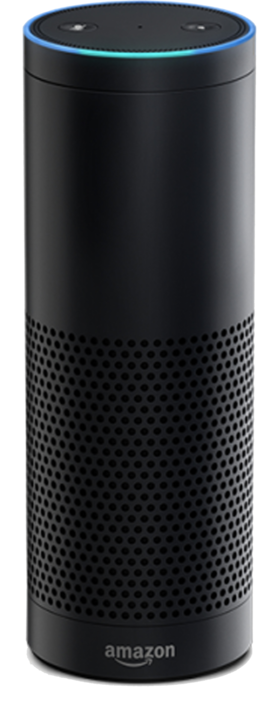
\includegraphics[height=6.6cm]{Graphics/3-3-Empirical-Home/Intro-AmazonEcho}} \quad \quad \qquad
    \subfloat[Google Home]
    {\label{fig:empirical home introduction smartspeakers googlehome}%
    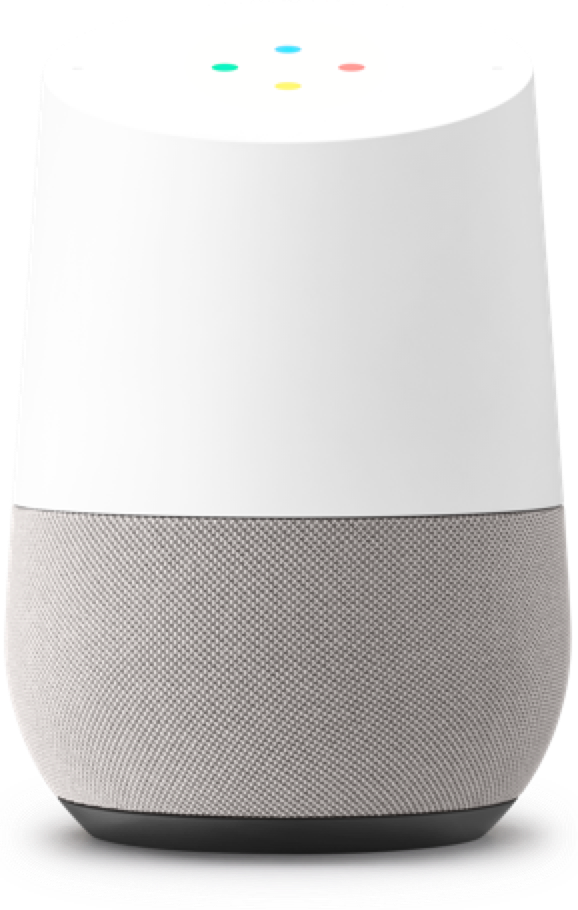
\includegraphics[height=4cm]{Graphics/3-3-Empirical-Home/Intro-GoogleHome}} \quad \quad \qquad
    \subfloat[Apple Homepod]
    {\label{fig:empirical home introduction smartspeakers homepod}%
    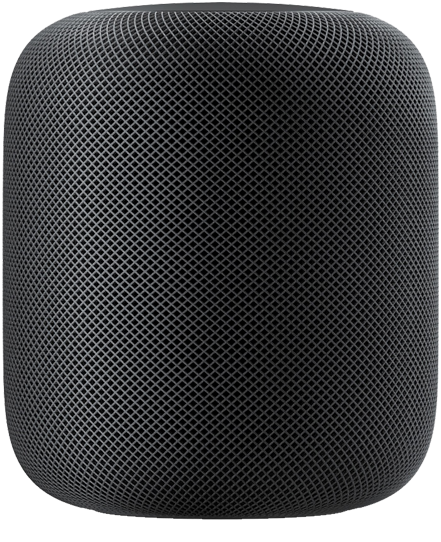
\includegraphics[height=4.3cm]{Graphics/3-3-Empirical-Home/Intro-AppleHomepod}}
    \caption[`Smartspeaker' devices are typically self-contained cylindrical speakers designed for the home.]{`Smartspeaker' devices are typically self-contained cylindrical speakers designed for the home. The images of the Amazon Echo, Google Home, and Apple Homepod are copyright Amazon.com, Inc.; Google Inc.; and Apple Inc. respectively. Images of models available in 2017.}\label{fig:empirical home introduction smartspeakers}
\end{figure}

Despite the wealth of enabling research in computational linguistics such as natural language processing, dialogue systems, and computational sociolinguistics~\citep{Nguyen2016}, research that empirically examines the social and interactional issues of \ac{VUI} use in an everyday home setting is lacking.
In other words, with a few exceptions, little is known about the practical accomplishment of interactions that solely take place with \acp{VUI}, or the articulation of just how those interactions unfold in the everyday lives of their users.
The prior work in this thesis (see \autoref{ch:empirical cafe}) unpacked this interaction in relation to use that takes place when the device interaction involved a portable personal device with a touchscreen, however, here this chapter instead explores \iresubmission{how members of a home make use of a device} when the device use is done entirely using voice.
This absence of literature is significant since the work outlined here suggests a range of conceptual shifts that might need to be taken into account when designing \acp{VUI} for home settings and, more broadly, multi-party interactions.
This work goes on to reveal further details of collaborative efforts by members to get the device to work in and through everyday talk, in line with the research questions posed in this thesis.

%This study draws on the traditions of \acf{EMCA} (see \autoref{ch:background emca}) to examine various ways in which the \ac{VUI} was implicated in talk.

%In the main part of this study, the ways in which the \ac{VUI} is embedded into the situational exigencies of the home are explored (such as other activities going on during use), and how its users account for the interactional work that this use involves.
%This chapter then moves on to look at the sequentially organised ways in which \ac{VUI} use is achieved in a multi-party conversational setting, and then concludes by discussing three key issues emerging from the findings: conceptual concerns regarding the framing of \ac{VUI} as `conversational' interaction; the ways that requests to \ac{VUI} are designed and the implication of accountability for this; and finally, the design of \ac{VUI} responses, and considering their role as interactional resources that users `go on' with.



% *********************************************************************************************************************


% \section{Research questions}\label{sec:empirical home rqs}
% This work, thus far, has unpacked numerous cooperative and collaborative activities around the use of portable touchscreen-based devices in casual-social settings.
% Such examples have included how members accountably sustain device use in and through conversation (\ref{sec:empirical pub discussion coop}) and the mutual production of silence following a request to a \ac{VUI} (\ref{sec:empirical cafe findings collab}).
% Here, this work moves onto considering how interaction unfolds in situations where voice is the only mode of interaction with the device.
% Furthermore, this work differs insomuch that it explores the use of devices as part of ongoing activities, i.e. this study will unpack how the use of \acs{VUI} is achieved and embedded within home life as multiple members of the have gathered:

% \PrintRQ{1}
% \PrintRQ{2}

% Furthermore, drawing upon RQ2, this work will go on to reveal further details that are explicated from the data of how members collaborate with each other.
% These \ac{VUI} devices under study embody two key characteristics that will impact how interaction with and around the device unfolds: (1) the devices pivot from being singularly controlled and owned by a single member to a communally controlled device controlled through any voice, where all members in the household can freely use the device, and it is owned by the household; and (2) the device does not provide a screen to denote how a prior request `went wrong', something that was used by members in their interaction with the device to resolve trouble (see \autoref{sec:empirical cafe findings multimodality}).



% *********************************************************************************************************************



\section{Study design}\label{sec:empirical home design}
\begin{revisedsubmission}[JR-2b: Include detail on the choice of setting and its connection to the technology use under study]
A brief description of the setting in which the studies were undertaken is provided below, including details about the participants involved.
This study deviates from the modus operandi established in the prior two empirical chapters in that the collection of data in this study is an audio-only longitudinal study in a non-public setting.
This section will introduce the rationale for this design as well as the reasoning for the continued adoption of an ethnomethodological analytic orientation (see \autoref{ch:background approach}).
The study was approved by the university's School of Computer Science Research Ethics Committee.
\end{revisedsubmission}



% *********************************************************************************************************************



\subsection{The home a study setting}\label{sec:empirical home design setting}
\begin{revisedsubmission}[JR-2b: Include detail on the choice of setting and its connection to the technology use under study]
Whereas the studies in Chapters \ref{ch:empirical pub} and \ref{ch:empirical cafe} focus on studying interaction in a semi-public `casual-social' setting (a pub and a caf\'{e} respectively), this exploration of standalone \acp{VUI} is conducted in participants' homes.
This is driven by the design of the device under study---whereas smartphones are engineered to be portable devices that allow users to achieve tasks irrespective of their location, `smartspeakers' are typically not designed to portable, need to be plugged in to mains electricity\footnote{Some portable standalone smartspeakers have since been released, such as the Amazon Tap, although none were available at the time of study and the Amazon Tap has since been seemingly discontinued.}, require configuration using an app to connect to a Wi-Fi connection, and are typically pitched by manufacturers as devices for the home.
With smartphones, their portability affords their use and thus the possibility of \textit{studying interactions around their use} in a range of different venues, with the ones chosen done so to explore how devices are used and interleaved within a multi-party conversation of friends socialising in a relaxed manner in a setting perspicuous to their use.
However, \acp{VUI} are not marketed as portable or \textit{personal}, but instead as communal devices that can be `installed' in a fixed location in the home, and usable by any person living in---or passing through---the space.

Despite the differences in design, including the lack of \acf{GUI}, the concept of the \ac{VUI} on a standalone device intersects with that of the \ac{VUI} on the smartphone: users use a `hotword', they deliver their request `using natural language'\footnote{This phrase is in quotes because its veracity is not established but proclaimed in the marketing materials of device manufacturers.}, and the \ac{VUI} responds through a synthesised voice that sounds humanlike\footnote{Relatively speaking, to an untrained ear, and within limits.} (note that in the case of smartspeakers, this synthesised voice is always produced whereas it is optional on portable devices).
Therefore, the lack of portability, personalness to an individual, and no \ac{GUI} establish the smartspeaker as a distinct but interrelated product to \acp{VUI} on smartphones, and establishes the need for studying the use of such a device in a home environment.
\end{revisedsubmission}



% *********************************************************************************************************************



\subsection{Collecting data in the home}\label{sec:empirical home design data}
In order to capture naturalistic use of a \ac{VUI} in the home, five households were recruited to take part in a month-long longitudinal study. 
\iresubmission*[J2-2b: Include details on the pertinence of the setting and technology choice]{The desire to adopt month-long longitudinal study approach instead of observing a gathering of friends as in the prior two studies stems from the both the design of \ac{VUI} smartspeakers being pitched as home-based devices and the recentness of the introduction to market of standalone smartspeakers.
While smartphones had been around for more than six years at the time of study in \autoref{ch:empirical pub} and \acp{VUI} had been found on smartphones for more than three years at the time of study in \autoref{ch:empirical cafe}, smartspeakers were less than two years old, and in the UK less than one year old at the time of this study.
A longitudinal study would potentially allow users to configure and develop \textit{some} competency in using the \ac{VUI} device rather than only focusing on their first encounters with a device\footnote{The only real requirement was that users had developed enough competency to be able to use the device, no measure of competency was taken or sought as the goal was not to determine or evaluate use over time.}.
}

Of the five households recruited for the study, three were inhabited by couples, while two households were families consisting of two parents and two children.
The age range of the adult participants spanned from late-20s to mid-50s.
Each participating household was given an Amazon Echo, configured with a household member's personal Amazon account, and the Alexa companion app was installed on one of their personal smartphones.
\iresubmission*[J2-2b: Include details on the pertinence of the setting and technology choice]{The purpose of this is to identify how the conversations unfold around the use of the \ac{VUI} in the designers' intended setting.}
Households freely selected the positioning of their Echo and could relocate it when and as desired.
Four of the households placed the \ac{VUI} in a kitchen or dining area, while one placed it in a living room.
\icorrection*[Added  reference to activity centres]{\label{line:activitycentres}These sorts of places, through the presence of the \ac{VUI} smartspeaker, are made into \textit{activity centres} and thus \textit{ecological habitats}.
\citet{Crabtree2003} define the former as ``places where media are actively produced and consumed and where information is transformed''~\citep[p. 215]{Crabtree2003} and the latter as ``places where communication media live and where residents go in order to locate particular resources''~\citep[p. 215]{Crabtree2003}.
The multiplicity of functions proffered by \acp{VUI} facilitates household members to make these devices `at home' (i.e. for their use to be part of the routine lived experience of those in the home rather than of some unusual occurrence)---to produce and consume media, as well as a site for communication\footnote{Although the Amazon Echo does include features for communication, such as voice calling, none was observed in these studies, perhaps given the relative nascency of the devices in the UK.}.}
%This chapter will reveal how the Echo is made at home as an \textit{activity centre}.}


\subsubsection{The Conditional Voice Recorder}\label{sec:empirical cafe design data cvr}
\begin{revisedsubmission}[J2-2b: Include details on the pertinence of the setting and technology choice]
Given the sensitivity and technical/ethical challenges of collecting data in the home over an extended period, this study further deviates from the previous studies by opting for audio collection only instead of video.
It was considered that recruiting participants to allow video capture in their home for an extended period would generate vast amounts of video data, including of many moments participants did not want to be recorded, as well as potentially being an invasive way of collecting data.
Solutions to this were considered, such as requiring participants to start and end recording, however, this would potentially impede the capture of any spontaneous interactions with the \ac{VUI} device.
Therefore, given the desire to study interaction in the home over a month-long period, this study further specifies that only interactions temporally close to the use of the \ac{VUI} should be studied, given the sensitivity to---and infeasibility of---analysing all interaction in the home.
\end{revisedsubmission}

To capture the use of the Alexa \ac{VUI} in the home, a second purpose-built device---termed the \acf{CVR}---was \iresubmission{designed, built, and} deployed with the Amazon Echo.
The \ac{CVR} is activated when a proximate Echo is used (the design of the \ac{CVR} is depicted in \autoref{fig:empirical home desig cvr}) by continually capturing audio using a conference microphone, i.e. it records voice \textit{conditionally} upon some event occurring.
The device always keeps the last minute of audio in a temporary buffer in the non-permanent memory of the device while active.
When the hotword, `Alexa' (that activates and begins the use of the \ac{VUI}) is detected, the \ac{CVR} saves the prior minute into permanent storage and records one further minute of audio (this period is extended if the hotword is heard in the subsequent minute).
The \ac{CVR} also features a button to turn off audio capture, and two LEDs (blue and red), that indicate when the \ac{CVR} is `listening' for the hotword (blue) and when it is recording (red).
The \ac{CVR} is more sensitive than the \ac{VUI}\footnote{Voice recognition systems often have an accuracy or threshold variable that allows a `best guess' of whether a particular sound fits a given word or not. In this case, the \ac{CVR} was prone to false positives such that it may sometimes activate recording when the user had not uttered the hotword. This was seen as favourable to false negatives, where the \ac{CVR} would not activate when the \ac{VUI} was used.}, to ensure talk to Alexa was captured.

\begin{figure}
    \centering
    \includegraphics[width=.7\textwidth]{Graphics/3-3-Empirical-Home/Design-ConditionalVoiceRecorder}
    \caption[External design of the Conditional Voice Recorder (CVR).]{The Conditional Voice Recorder (CVR) is a small (12cm by 12cm) black box with a white lid. On the lid is a conference microphone, two LEDs (one blue, one red; to indicate when the \ac{CVR} is actively 'listening' for the hotword and when it is recording, respectively), and a button to turn on, or off, the CVR. Pictured also is the bottom part of an Amazon Echo. Version 2 of the \ac{CVR} is shown (Version 1 being an initial developmental prototype).}\label{fig:empirical home desig cvr}
\end{figure}



% *********************************************************************************************************************



\subsection{Analysing the collected data}\label{sec:empirical home design analysis}
\iresubmission[JR3a, ER-G1: Add further information about the analysis of the corpus, including the selection of fragments]{The resulting corpus of data from the deployments consists of over 6 hours of recorded data, where each audio clip consists of one or more requests to the \ac{VUI} in the home, as well as the preceding and succeeding conversation around the request.}
Overall, 883 distinct `request' utterances have been identified, where a request is talk that is directed to the \ac{VUI} in a seeming attempt to get it to `do something', e.g. answer a trivia question, play particular music, or set a timer.
Often these requests formed part of a larger sequence which might encompass various other requests that are temporally and/or topically related.
The corpus contains 185 of these (i.e. there are 185 audio clips containing the use of the \ac{VUI}).

\begin{revisedsubmission}[JR-3a: Change EMCA to `study informed by EM']
As with the previous chapters, this work takes on the perspective of ethnomethodology and is interested in how members organised their actions with and around the \ac{VUI}.
Specifically, this work examines how members, as conversationalists, analysed moment-by-moment unfolding interactions with and around the device and with one another to accomplish and address the problem that occasioned the use of the \ac{VUI}.
\end{revisedsubmission}

\iresubmission*[ER-G1: Add further information about the analysis of the corpus, primarily the selection of fragments]{A substantive review of the audio clips was performed to document the requests to the \ac{VUI} and who made them.
Twelve fragments were then transcribed carefully using the Jeffersonian transcription system (see \appref{app:notation}).
These fragments were selected in line with the aims of this research to reveal the ways in which members use a standalone \ac{VUI} device in and through conversation (in other words: each clip focused on the use of the \ac{VUI} while other people where audibly co-present).
Although there was interest in situations where the \ac{VUI} was used solitarily, this is beyond the focus of this thesis' aim to study the use of technology during gatherings of multiple people and of the naturally accountable interactions around this use (see~\ref{line:naturalaccountability} on natural accountability).
It was determined that each fragment selected warranted further investigation, with each fragment being reviewed individually and discussed collaboratively with other researchers multiple times.
The fragments selected for inclusion in this thesis `vividly exhibit'~\citep{Bannon1993} the interactional accomplishments of the members in selecting to use the \ac{VUI}, as exemplars of the data in the corpus~\citep{Crabtree2012}, but are not representative of how all instances of \ac{VUI} use may unfold.}

%Based on the findings in \autoref{ch:empirical cafe}, it was expected that various conversational methods would come into play and be adapted so as to `get stuff done' with the \ac{VUI}.
%The use of \acf{VUI} as a tool for unpacking the sequential and embedded practice of situated actions is an established technique in \ac{HCI} (e.g. \citet{Gilbert1990}), but it is noted that this work does not seek to treat the device as a \textit{participant} in conversation (see the discussion in the prior empirical chapter, \ref{sec:empirical cafe discussion humanlike}).

%The fragments of data presented in this chapter draw upon the transcript notation in \appref{app:notation}.
All names and identifiable information within the transcripts are, as before, entirely fictional.
%Some counting is provided throughout the findings to give an understanding of the commonality for which different aspects of \ac{VUI} use occurred.
%However, these should be treated as descriptive indices and not quantitative findings.
Talk that appears primarily to be addressed to the \ac{VUI} by members of the setting is highlighted in bold text.
In turn, the synthesised voice produced by the \ac{VUI} is identified by the label `ALE' (i.e. ALExa) in transcripts.
The inclusion of synthesised voice output as part of the transcript should not be seen to suggest any conceptual equivalence among members and the \ac{VUI}, but merely constitutes a convenient way of presenting the temporal organisation of device output as it appears in interaction.

%The fragments examined in this chapter are taken from one family living together in a household, and in particular, during their use of the \ac{VUI} while consuming family meals.


%Inspired by a similar line of approach to \citet{Reeves2016}, this work looks at the family's interactions in two interconnected ways.
%Firstly, the ways in which the \ac{VUI} is made `at home' and embedded into the various activities of home life are examined.
%Secondly, this chapter turns to unpacking how the \ac{VUI} features in \textit{sequential courses of action}, i.e. the orderly production of conversation.



% *********************************************************************************************************************



\section{Findings}\label{sec:empirical home findings}
\iresubmission[JR-3a, JR-3c: Introduce the fragments, two of which are different to the prior submission]{Data from the fieldwork will now be introduced and presented over a series of data excerpts. %---these fragments are \textit{vivid exhibits}~\citep{Crabtree2012} of the data within the collected corpus.
The fragments revealed in this chapter are taken from two different households over three different occasions.
The first fragment examines how users test the \textit{functionality} of a \ac{VUI}, as per \ref{sec:empirical cafe findings capability} with smartphone-based \acp{VUI} (see \ref{sec:empirical home findings capability}), and provides a clear sense of the nature of interaction with a \ac{VUI} device.
The second further introduces how the use of a screenless-\ac{VUI} device is done accountably to the normative moral order of the setting, in this case to ask for background music suitable to a New Year's Eve party.
Whereas the first fragment reveals little of the social interaction around the \ac{VUI}, this second fragment  progressively emphasises the intricate nature in which \acp{VUI} are used, with the different sorts of activities that take place around their use.
The third fragment introduced in this chapter reveals how the design of a \ac{VUI} smartspeaker supports their use for long-running activities while those collocated are also performing another task together (in this case, eating a family meal while playing a game together), bringing in the richness of the setting and how \ac{VUI} devices are used as part of the multi-activity home.}
Interaction with the device will be shown not to take place as a singular indiscriminate event but rather is achieved as a situated action as part of---or rather, \textit{interleaved} within---the already ongoing activities that unfold within the home.
\begin{revisedsubmission}[ER-G1: Add further information about the analysis of the corpus, primarily the selection of fragments]{
In this sense, and by design, the home is regarded as---and will be shown to be---a perspicuous setting~\citep[p. 181]{Garfinkel2002} for the use of \ac{VUI} devices and thus the examination of their use.}

%\appref{app:notation} provides details of the transcript notation used in this thesis.
%All names and identifiable information within the transcripts provided are entirely fictional.

%The family are selected for analysis as a single case~\citep{Schegloff1987} to provide a series of ``vivid exhibits''~\citep{Bannon1993} of the broad array of methods members employ across the corpus.

As before in the prior empirical chapters, this work is not interested in claiming that these are `representative' or `generalised' findings of how all interactions can or may unfold; rather, it is given that members continually try to make their own interactions orderly and rely upon the orderly features of others so as to each analyse what the others are doing and thus `go on' (the \textit{ethnomethodological perspective}, see~\autoref{ch:background approach}).
This means that this chapter, as with the prior two, seeks to exhibit how members bring the \ac{VUI} device practically into that interaction order.
\end{revisedsubmission}



% *********************************************************************************************************************



\subsection{Establishing the capability of a VUI}\label{sec:empirical home findings capability}
\begin{revisedsubmission}[JR-3a, JR-3c: This section is new, constructed from previously collected data]
This first fragment, called \textit{Where is Greece?}\footnote{The complete fragment is included in \appref{app:fragments-home greece}.}, commences in \autoref{frag:empirical home findings capability-i}.
This excerpt unfolds as the two homeowners, Nikos and Isabel, are entertaining their neighbours, Leah and John, who are chatting and socialising around the bar in the kitchen area of their flat.
Nikos introduces the Amazon Echo and then Leah and John take turns using the device, asking it various questions.
%We join the action as Leah asks ``where is greece?'', establishing her request to determine how a device without a screen responds to requests for the location of places.
All participants in the conversation are Greek, and at times converse in Greek and sometimes in English (primarily towards the Amazon Echo).
Talk that was Greek in these conversations was translated into English by Nikos following the study.

Previously, in \ref{sec:empirical cafe findings capability}, establishing the functionality of a smartphone-based \ac{VUI} was shown to consist of two actions by members, and indeed the same actions are revealed to take place with the screenless \ac{VUI} device when unpacking the actions of members:
\begin{enumerate}[label=(\roman*)]
\item \nameref{sec:empirical home findings capability establish}, and
\item \nameref{sec:empirical home findings capability testing}.
\end{enumerate}

These activities are now explicated in the following two sections, revealing the problem case of whether the device is able to deal with requests for the details of places.
\end{revisedsubmission}



% *********************************************************************************************************************



\subsubsection{Establishing the desired function}\label{sec:empirical home findings capability establish}
\begin{revisedsubmission}
We join the action in \autoref{frag:empirical home findings capability-i} as the friends are sitting down to drink coffee in the kitchen area of the flat.
John, one of the guests, has asked a number of questions to the device regarding definitions of words, a well-advertised feature of the Amazon Echo.
After requesting a few words, Leah takes a turn in conversation and introduces a request for a different type of request: one for details of a specific location.
\end{revisedsubmission}

\begin{inlinefrag}
    {\fragresubmission{JR-3c, ER-H: This is a new fragment from the existing corpus}
    \begin{transcript}
        \by LEA {\textbf{alexa (.) where is greece}} \\
        \later   {2.0} \\
        \by ALE {\textit{// greece is a un-recognised country in the northern hemisphere}} \\
        \by     {\textit{(.) it shares a border with turkey, albania, bulgaria}} \\
        \by     {\textit{and macedonia= //}} \\
        \by ISA {~~~~~~~~~~~~~=[ that’s it ]} \\
        \by LEA {~~~~~~~~~~~~~=[ that’s it ]} \\
    \end{transcript}
    \caption{Where is Greece? (i)}\label{frag:empirical home findings capability-i}
    }
\end{inlinefrag}

\begin{revisedsubmission}
In this opening excerpt, Leah makes the request to the \ac{VUI} for \QF[01]{where is greece?}.
Given the \ac{VUI} is screenless, this request is positioned not as a `show me on a map', but rather a request for a description of the location of the country Greece.
The members do not talk as the \ac{VUI} delivers its response, listing the neighbouring countries of Greece and upon the device remarking that Greece neighbours Macedonia, both Isabel and Leah simultaneously remark \QF*[06--07]{that's it}.
All four friends in the room, of course, \textit{know} the location of Greece---as they are all Greek---the request is merely to explore the capability of the device to support sense-making in how the device responds to various requests.
The remark of \QF{that's it}, delivered jointly by Leah and Isabel latches on the completion of the name \QF[05]{macedonia} by \ac{VUI}, and turns upon a geopolitical dispute between the nations of Greece and the Republic of Macedonia, and brings to the fore how members of the setting are waiting for the name to be produced as part of the list of neighbouring countries\footnote{This was verified through discussion with the participant household members following the study.}.

In performing this request, Leah establishes the premise that her request is to test the capability of the \ac{VUI} to respond to questions about the location of places.
In choosing to request details of a location of which she is acutely aware, she reveals that her request is both to determine whether the device supports \textit{this kind of request}, and further enable her to establish the veracity of the response from the \ac{VUI}.

Of course, Leah does more than establishing the desired function of the \ac{VUI}, she \textit{tests} its functionality too, by addressing the device with her request.
In other words, Leah's address to the \ac{VUI} performs both the work of \textit{establishing} and \textit{testing} it.
The next section expands upon the notion of testing a \ac{VUI} by examining two further questions put to the device.
\end{revisedsubmission}



% *********************************************************************************************************************



\subsubsection{Testing the functionality by addressing the VUI}\label{sec:empirical home findings capability testing}
\begin{revisedsubmission}
Following Leah's opening request to establish and question the device to give information regarding the location of places, John proceeds to ask a further question in the same vein.
In this next exhibit, found in \autoref{frag:empirical home findings capability-ii}, John asks the \ac{VUI} for the location of \textit{Amfissa}, a city in Greece.
\end{revisedsubmission}

\begin{inlinefrag}
    {\fragresubmission{JR-3c, ER-H: This is a new fragment from the existing corpus}
    \begin{transcript}[9]
        \by JOH {\textbf{alexa where is amfissa}} \\
        \later  {2.0} \\
        \by ALE {\textit{// amfissa is a city in phocidos (..) greece (.) it is 82 miles}} \\
        \by     {\textit{133 kilometres west of athens and 26 miles 42 kilometres south}} \\
        \by     {\textit{of lamia //}} \\
    \end{transcript}
    \caption{Where is Greece? (ii)}\label{frag:empirical home findings capability-ii}
    }
\end{inlinefrag}

\begin{revisedsubmission}
In this second excerpt, John follows the same structure in his request to the device as Leah (i.e. \textit{where is\ldots}), but this time asks for the location of a city in Greece, and could be considered to be `upping the ante' by asking a question that is ostensibly more difficult given its specificity of being a city rather than country.
In this instance, as with the prior request, the device responds seemingly correctly with the members in the setting allowing the device to complete its response.

Following this response, John makes a further attempt at \textit{testing the functionality of the \ac{VUI}}, as depicted in \autoref{frag:empirical home findings capability-iii}.
As before, he does this by following the same format of request as established by Leah (i.e. \textit{where is}), but this time opts to ask the \ac{VUI} device for the location of \QF[15]{delphi}\footnote{This is spelt \textit{delph-ee} in the fragment transcript to distinguish it from the different pronunciation used by the \ac{VUI} device in its response of \textit{delph-i}.}.
\end{revisedsubmission}

\begin{inlinefrag}
    {\fragresubmission{JR-3c, ER-H: This is a new fragment from the existing corpus}
    \begin{transcript}[15]
        \by JOH {\textbf{alexa where is (0.3) delph-ee}} \\
        \later  {7.0} \\
        \by ALE {\textit{// delph-i is a village in carroll county indiana (.) indiana (.)}} \\
        \by     {\textit{it is 62 miles 99 kilometres north of Indianapolis and 87 miles}} \\
        \by     {\textit{140 kilometres= //}} \\
        \by NIK {~~~~~~~~~~~~~~~\textbf{=alexa stop}} \\
    \end{transcript}
    \caption{Where is Greece? (iii)}\label{frag:empirical home findings capability-iii}
    }
\end{inlinefrag}

\begin{revisedsubmission}
In the first excerpt in this fragment, Leah asks the \ac{VUI} device for the location of \textit{Greece}, the country she and other co-interlocutors are from.
In this, she establishes her desire to determine how the device provides information about the location of places and chooses a place of which she is aware---in this case, her country of origin.
This notion is further realised through the successive utterances produced in the setting (the retrospective-prospective character of action, see \ref{sec:background approach em sequentiality})
The second request to the \ac{VUI} smartspeaker, by John, her partner, further tests the \ac{VUI} by increasing the specificity of the locale put to the device to locate.
In both cases, ostensibly, the device responds as members seemingly expect.
In this final excerpt, John asks for the location of \QF[15]{delphi}, which is an ancient monument and a registered UNESCO World Heritage Site in Greece.
With this, it seemingly becomes evident that John's follow up question is asking for the location of something more precise than the prior two questions (country and then city), and further establishes the ratcheting of specificity over the three requests to the device in this fragment.

After John's request, the \ac{VUI} device takes 7 seconds to respond, during which the members remain quiet\footnote{Given \acp{VUI} devices of this nature do not verbalise what-it-is-doing, it is unclear as to the cause of this elongated time between request and response.}.
The device begins responding, and commences its response with a different pronunciation of the place requested by John (delph\textit{ee} vs. delph\textit{i}), and gives the location of a village in Indiana, USA.
Given the coherence and context established through the production of the prior two requests to the device, it is determined that this response from the device is not the intended location of which John was seeking details.
Nikos cuts the \ac{VUI} device off as it continues to produce information about Delphi, Indiana by producing the request \QF[20]{alexa stop}.%---the group stop using the device to get the details of locales.

The group discussion then moves on to new topics after this response, affirming this sequence of events was around the purpose of \textit{testing the functionality of the \ac{VUI}} rather than actually seeking information about the location of a country, city, and landmark.
With smartphone-based \acp{VUI}, establishing the capability of the \ac{VUI} was positioned as a case that deviated from actions performed typically with touchscreen-based devices, as the \ac{VUI} features were made available to users in the past few years.
Moreover, in the context of the screenless devices, which were released within the UK within the prior three months before the recording of this fragment occurred, establishing the capability of the \ac{VUI} was a recurrent practice amongst all the households studied.
\end{revisedsubmission}



% *********************************************************************************************************************



\crpagebreak\subsubsection{Methodical accomplishments in this fragment}\label{sec:empirical home findings capability methods}
\begin{revisedsubmission}
In this first fragment, the work of establishing the capability of a smartspeaker \ac{VUI} to respond to \QF{where is} questions is unpacked.
Leah initially opens the \textbf{address to the \ac{VUI} by using the hotword, followed by her request}.
Through the member's perspective, this request is establishing and testing the functionality of the \ac{VUI}, given that Leah knows the answer to the question.
The \ac{VUI} computes a response for a few seconds, and the co-present members \textbf{do not talk until the \ac{VUI} has fully delivered its answer} through a synthesised voice.
A second request is produced by another member through \textbf{address to the \ac{VUI}}, using the same wording but with a more specific location (i.e. a `harder' question, and again this turns upon the members of the setting being knowledgeable of the correct answer).
Again, the \ac{VUI} computes and responds to this request through the synthesised voice.
A third request that is ostensibly more difficult again is \textbf{addressed to the \ac{VUI}} by the same member.
The \ac{VUI} takes seven seconds to compute an answer and begins to deliver its response, using a different pronunciation of the locale given by the user.
The coherence of the questions establishes that this answer from the \ac{VUI} is `incorrect' (i.e. for a different location with the same spelling), and is reinforced by another member of the setting \textbf{cutting off the \ac{VUI}'s response delivery by addressing it with a stop command}.
Through the perspective of the members, this sequence of requests is about establishing and testing the capability of the \ac{VUI}---not to literally find the location of Greece, Amfissa, and Delphi.
The interactional project was a success from this perspective.
\end{revisedsubmission}



% *********************************************************************************************************************



\subsection{Asking the VUI to play music}\label{sec:empirical home findings music}
\begin{revisedsubmission}[JR-3a, JR-3c: This section is new, constructed from previously collected data]
This second fragment, called \textit{New Year's Music?}\footnote{The complete fragment is included in \appref{app:fragments-home nye-music}.}, commences in \autoref{frag:empirical home findings music-i}.
This excerpt unfolds as the same two homeowners as above, Nikos and Isabel, are hosting a New Year's Eve party.
The party has been going for some time and during a conversation about the Amazon Echo and the \ac{CVR}, an attendee commences the interactional project of playing some background music using the Amazon Echo.
One of the key marketed features of the Echo is the ability to perform long-running tasks such as playing music or setting timers.

In this fragment, a guest, Anna, will be facilitated in making a request to the device by Nikos, however, the request ultimately fails and the two users attend to dealing with the outcome of the device's computation.
This fragment will progressively demonstrate the ways in which interaction with a \ac{VUI} occurs within and is accountable to others within the setting.

Overall, the members' problem of getting the device to play music in the background will be shown to consist of two core activities that will be unpacked across a number of excerpts:
\end{revisedsubmission}
\begin{enumerate}[label=(\roman*)]
\item \nameref{sec:empirical home findings music requesting}, and
\item \nameref{sec:empirical home findings music responding}.
\end{enumerate}



% *********************************************************************************************************************



\subsubsection{Requesting the VUI to play a category of music}\label{sec:empirical home findings music requesting}
\begin{revisedsubmission}
Firstly, the request to the \ac{VUI} device to play music is examined.
This request is presented in \autoref{frag:empirical home findings music-i} and occurs amongst the hubbub of the party in the background.
Nikos, the homeowner, opens the interaction with the Echo by producing the hotword, before Anna performs a request for the device to play music.
\end{revisedsubmission}

\begin{inlinefrag}
    {\fragresubmission{JR-3c, ER-H: This is a new fragment from the existing corpus}
    \begin{transcript}
        \by NIK {\textbf{alexa}} \\
        \later  {2.6} \\
        \by ANN {\textbf{play some new year’s music}} \\
        \later  {1.8} \\
        \by ALE {\textit{// here’s a station for jazz music (.) instrumental jazz //}} \\
        \by     {\textit{((begins playing jazz music))}}
    \end{transcript}
    \caption{New Year's Music (i)}\label{frag:empirical home findings music-i}
    }
\end{inlinefrag}

\begin{revisedsubmission}
The first consideration in examining this fragment is the categorisation of music that Anna uses---specifically that of \QF[03]{new year's music}.
This categorisation does not a carry specific genre or type of music connotation, yet of course, remains a normatively understood request to be for music suitable for a New Year's Eve party.
This illuminates a key consideration of how users approach such devices: given there is no reference for correct use of the device\footnote{By \textit{correct use} this thesis means \textit{gets the device to do the desired function}, i.e. it is the correct outcome from the user's perspective.} or input to the device (i.e. there is no \textit{a priori} information as to what works, or does not work), users must produce utterances that may or may not work to determine the capability\footnote{In contrast to a \ac{GUI} which could display possible next options.}.

Specifically in this case, \QF{new year's music} turns upon various socially shared and culturally situated assumptions about what constitutes relevant music to play for New Year's Eve.
As members of society, we routinely deal with and attend to such complexities of categorisation\footnote{Nikos does not challenge or guide Anna to expand upon her choice of music.}, yet such challenges are not pre-determinedly defined, such as a codified genre or specific artist or song, but rather music relevant to a season or holiday. %\footnote{Design of conventional \ac{VUI} is ostensibly script-based with variations in produced sentences to avoid repetition.}
The device responds to this request by playing \textit{instrumental Jazz music}, although in the opaqueness of the device, it remains unclear whether the device has understood `correctly'.
A later examination by the researcher of the web-based logs available to Amazon Echo users revealed a request for ``play jazz music'', suggesting\footnote{Although not \textit{confirming}, as the veracity of such cannot be established.} that the device did not correctly transcribe the spoken input.
\end{revisedsubmission}



% *********************************************************************************************************************



\subsubsection{Responding to the VUI's choice of music}\label{sec:empirical home findings music responding}
\begin{revisedsubmission}
The next element of this fragment is to consider how Anna responds to the device's next action to play \QF[05]{instrumental jazz} music.
The next excerpt, \autoref{frag:empirical home findings music-ii}, commences as she does so.
\end{revisedsubmission}

\newpage
\begin{inlinefrag}
    {\fragresubmission{JR-3c, ER-H: This is a new fragment from the existing corpus}
    \begin{transcript}[12]
        \by ANN {\textbf{alexa this is not what we wanted}} \\
        \by     {[ ((laughs))~~~~~~~~~~~~~]} \\
    \end{transcript}
    \caption{New Year's Music (ii)}\label{frag:empirical home findings music-ii}
    }
\end{inlinefrag}

\begin{revisedsubmission}
This second excerpt brings to the fore a key element of interaction with \acp{VUI} through deepening Anna's response to the device's next action.
First of all, it becomes evident that to Anna \QF{new years music} does not include the \QF{instrumental jazz} station the Echo has opted to play.
She attends to this matter by using the hotword to activate the device and says \QF[12]{this is not what we wanted}.
In furthering the previously established point regarding the use of voice-based interfaces being used with various socially agreed categorisations, it may be suggested that the current design of \acp{VUI} necessitate a try-and-see approach.
Consider this instance in the context of both the prior fragments in this chapter (see \ref{sec:empirical home findings capability}) and the use of the smartphone-based \ac{VUI} to explore device capability (see \ref{sec:empirical cafe findings capability}): in all three instances, the practice adopted by users is that of making an attempt at doing something to \textit{understand if an option is possible}.
This underscores an intrinsic difference in the way devices get to be used for various tasks: typically \acp{GUI} present available options to users through menus, graphics, icons, and so forth; however a \ac{VUI} provides little in the way of \textit{affordance} to guide the user\footnote{Here the use of \textit{affordance} is more in accord with \citet{Norman1988}'s use of the term, i.e. an affordance provides ``strong clues for the operation'' of the item~\citep[p. 9]{Norman1988}, rather than \citet{Gibson1979}'s original definition.} resulting in a \textit{trial-and-error} approach: users must issue requests to determine \textit{if and how the device would respond} in order to determine \textit{what the correct input is for the device to respond the way they want, if it exists}.

A third excerpt, \autoref{frag:empirical home findings music-iii}, is now introduced that incorporates the prior excerpt (for readability), but also includes the interaction that follows Anna's remark that the music is not what she desired, followed by laughter.
\end{revisedsubmission}

\begin{inlinefrag}
    {\fragresubmission{JR-3c, ER-H: This is a new fragment from the existing corpus}
    \begin{transcript}[12]
        \by ANN {\textbf{alexa this is not what we wanted}} \\
        \by     {[ ((laughs))~~~~~~~~~~~~~]} \\
        \by NIK {[ (1.2) \textbf{alexa} (1.1) \textbf{shut} ] \textbf{up!}} \\
        \by ANN {hey::\intUp (.) \textbf{alexa nikos apologises for being so rude}} \\
        \later  {0.3} \\
        \by ALE {hi there} \\
        \by     {[ \textit{((resumes playing jazz music)) }]} \\
        \by NIK {[ (2.4) \textbf{alexa stop} ~~~~~~~~~~~~~~] \textbf{stop!}} \\
    \end{transcript}
    \caption{New Year's Music (iii)}\label{frag:empirical home findings music-iii}
    }
\end{inlinefrag}

\begin{revisedsubmission}
In this final excerpt from the fragment, the device does not respond to Anna's request, following which Nikos then instructs the \ac{VUI} to \QF[14]{shut up}, a command that stops the playback of music on the device\footnote{The \ac{VUI} responds to this command in much the same way as the command \textit{stop}. The two most common \ac{VUI} devices, Amazon Echo and Google Home, now include a child-friendly mode that primarily only responds to `polite' requests from users, although this did not exist at the time of the study.}.
Given the accountable nature of interaction with a \ac{VUI} device---in that talk to and from the device is audible and reportable by those present, talk to the device exists and can be called to account within the normative moral order of the setting.
In the excerpt, Nikos tells the device to \QF[14]{shut up}, to which Anna produces an ostensibly ironic apology to the device for the rudeness of his response \QF[15]{nikos apologises for being so rude}, and in doing so establishes the viewpoint that Nikos' request to the device breached the normative moral order---i.e. the socially shared and agreed-upon sets of ways of acting---against which members of the setting are held to account.
In this indirect rebuke, Anna enforces the notion that the use of the \ac{VUI} occurs within this normative moral order, and in turn, that the device itself becomes embedded within the fabric of the home, through the established and expected moral organisation of social conduct.
In other words, the \ac{VUI} smartspeaker does not exist as a personal or private device, but one for which its use is considered an activity that is accountable to all in the home.
\end{revisedsubmission}



% *********************************************************************************************************************



\subsubsection{Methodical accomplishments in this fragment}\label{sec:empirical home findings music methods}
\begin{revisedsubmission}
This second fragment examines the interactional project of requesting a \ac{VUI} to play some music.
During a party, a discussion ensues about playing some background music.
The homeowner, Nikos, \textbf{addresses the \ac{VUI} by uttering the hotword} to activate it, following which a guest, Anna, \textbf{addresses the \ac{VUI} with a request for appropriate music}.
The \ac{VUI} computes and then responds to the request with a synthesised voice describing its next action---to play instrumental jazz music.
Anna again \textbf{addresses the \ac{VUI}}, by producing the hotword and \textbf{stating that the outcome was not as they desired}.
The \ac{VUI} does not respond within a second or so to this address, following which Nikos then \textbf{addresses the \ac{VUI} by instructing it to \QF{shut up}}.
This address leads to Anna \textbf{reprimanding Nikos} by rhetorically \textbf{addressing the \ac{VUI} again that Nikos \QF{apologies for being so rude}}.
The \ac{VUI} produces a response that does not seem to coherently follow from any of the three prior requests addressed to it.
After the \ac{VUI} resumes playing music, Nikos \textbf{cuts off the \ac{VUI}'s playback} through a further \textbf{address of instructing it to stop}, thus ending the interactional project to play music using the \ac{VUI}.
\end{revisedsubmission}



% *********************************************************************************************************************



\subsection{Using the VUI to play a game while eating}\label{sec:empirical home findings game}
\begin{revisedsubmission}[JR-3a, JR-3c: This section is new, constructed from previously collected data]
To briefly recap, the first fragment introduced how \ac{VUI} devices are used within conversations in homes to respond to various requests for information, as users test and explore the functionality of the device through use.
The second fragment deepened this explication of how \acp{VUI} are used within the home, revealing elements such as how users may select socially-established definitions in their requests rather than typical \textit{a priori} discrete categorisations; and further how \ac{VUI} use is held to account within the setting.

The final fragment, called \textit{Beat the Intro}\footnote{The complete fragment is included in \appref{app:fragments-home beat-the-intro}.}, is from a family consisting of two parents, Susan and Carl, and two children around ten years old, Liam and Emma; and further demonstrates how \ac{VUI} devices are brought into an ongoing  activity in the home, but more so function as multi-user devices within the multi-activity home.
In this sense, the \ac{VUI} device is shown to be used in and around conversations in the home.
In this home the \ac{VUI} is placed on the top of a bookcase that is used as a sideboard in the dining room.
The family have been using the Amazon Echo for approximately a week, and have developed a reasonable familiarity and competence in its use, with each member of the household having used the Echo for most days at least once or twice.
They are eating an evening meal all together at the dinner table on Mothers' Day.

This problem of getting the device to play a game while the family are eating a meal is unpacked over the following three activities, with the former establishing how the \ac{VUI} becomes introduced into an ongoing activity in the home:
\begin{enumerate}[label=(\roman*)]
\item \nameref{sec:empirical home findings game preinit},
\item \nameref{sec:empirical home findings game address}, and
\item \nameref{sec:empirical home findings game responding}.
\end{enumerate}

\end{revisedsubmission}



% *********************************************************************************************************************



\subsubsection{Preparing to address the VUI}\label{sec:empirical home findings game preinit}
As we join the family in the first excerpt, \autoref{frag:empirical home findings game-i}, Susan, the mother, announces to the others that she would like to play Beat the Intro \QF[01]{in a minute}.

Beat the Intro is a game available for the Amazon Echo that the family have previously played together; it involves listening to a few seconds from the start of a song and then players must guess, by announcing, the song and the artist.
The game is a `Skill'---an installable feature developed by a 3rd-party for the Amazon Echo.

\begin{inlinefrag}
    \begin{transcript}
        \by SUS {i'd like to play beat the intro in a minute} \\
        \by LIA {[ oh no:: ]} \\
        \by SUS {[ \textbf{alexa}~~~][ (1.1)~~] \textbf{beat the in}[\textbf{tro}} \\
        \by CAR {~~~~~~~~~~~[ \quiet{yeah} ] } \\
        \by LIA {~~~~~~~~~~~~~~~~~~~~~~~~~~~~~~~~~[°no:::...°} \\
        \later {0.6} \\
        \by CAR {it's mother's day?} \\
        \later {0.4} \\
        \by SUS {it's (~~~~) yep (.) listen (.) you need to keep on eating your} \\
        \by     {orange stuff (.) liam} \\
        \later {0.7} \\
        \by CAR {and your green stuff} \\
    \end{transcript}
    \caption{Beat the Intro (i)}\label{frag:empirical home findings game-i}
\end{inlinefrag}

\iresubmission{Susan announces to the family that she would like to \QF[01]{play beat the intro}, and in doing so, prepares the family to play a game together using the \ac{VUI}.}
Liam produces an assessment of this (\QFt[02]{oh no}) and then an elongated \QF[05]{no} as Susan then instructs the \ac{VUI} to play the game.
Carl mentions Mother's Day, while Susan instructs Liam to eat his food.
%Susan then attempts another instruction to Alexa to \QF[15]{play beat the intro}.

The first observation is that addressing the \ac{VUI}---here located in instructions to play the Beat the Intro skill---is \iresubmission{interleaved} amongst \textit{multiple activities}, or `courses of action', that the family are working to accomplish together.
For instance, the family are eating dinner together, and they are talking about that eating (lines 09--12 particularly).
Requests for compliance from Liam are produced by Carl amongst Susan's initial instruction to the \ac{VUI} (line 03), where Carl counters Liam's negative response to Susan's preparatory utterance \QF[01]{i'd like to play beat the intro in a minute} with the reminder that \QF[07]{it's mother's day?}.
Activities that might be glossed broadly as `parenting' turn on establishing appropriate ways of behaving during mealtimes particularly for younger members of the family, such as the instruction to Liam to \QF*[09--10]{keep on eating your orange stuff}.
All the while, these other concurrent activities are closely geared into the organisation of Susan's further requests to the \ac{VUI}.
%For instance, Susan's second instruction commencing on line 13, is interleaved with Carl's continuation of Susan's prior request to Liam to eat his food.
%Carl provides a series of \textit{and}-prefaced turns (\QFt[12]{and your green stuff}; and \QFt[14]{and your brown stuff}).

\begin{revisedsubmission}
It is through these `other' utterances---not to the device, but to each other---around which the \ac{VUI} is used, that establishes the family's treatment of playing a game with the \ac{VUI} during dinner with perspicuity.
In this sense, the activity is not oriented to as unusual or out-of-place, merely \textit{unwanted} by some members because of their inevitable involvement.
Furthermore, here, the action of preparing others for the use the device as a family for a cooperative activity demarcates this \textit{type} of device as different to smartphones, insomuch that here the smartspeaker is to be used \textit{together} by the family, and that this preparatory account is used to ready the members for the next action Susan is to perform (i.e. that she, and the family, are to play Beat the Intro together).

Another issue to consider is how the \ac{VUI} device responds to the user, and whether this is treated as a \textit{success} in the course of action by the users.
In the first fragment examined in this chapter, the device provided information on the incorrect \textit{Delphi} (USA, as opposed to Greece) and in the second fragment, the device provided the wrong sort of music as an issue in transcribing spoken words into text; in this excerpt, however, a different type of technical problem occurs in comparison to the prior two fragments: no-response.
In this sense, it remains unclear as to the specific nature of the problem at hand and provides no information as to the actions the user (or as shall be revealed, \textit{users}), should take.
\end{revisedsubmission}

In many ways, these initial observations offer a consonance with prior studies of technology use in the home and how such technologies get drawn into the organisation of home life as resources for action (e.g. see \citet{Rooksby2015}).
Empirical accounts such as these present a more nuanced perspective to the conceptualisation of such technologies like the \ac{VUI} as disruptive to established moral order by drawing attention away from interaction with co-present others~\citep{Turkle2011}---rather, here it can be seen \iresubmission{that what is unfolding is the use of the \ac{VUI} alongside other ongoing activities, suggesting that} \ac{VUI} devices get recruited into the lifeworld of cooperative and collocated activities in the home~\citep{Rigby2017,Rooksby2015,Tolmie2008}.
In this sense, the use of these devices becomes regulated \textit{in} those activities.



% *********************************************************************************************************************



\subsubsection{Requesting the game}\label{sec:empirical home findings game address}
\begin{revisedsubmission}
The next matter to turn to is the address to the \ac{VUI}, and for this a further excerpt of data is presented in \autoref{frag:empirical home findings game-ii}.
A request has already been made on line 03 above, although this has ostensibly `not worked' by virtue of the device not responding to the request.
In this next excerpt, the matter of how members in the setting embed this request amongst the ongoing activity in the home is examined.
\end{revisedsubmission}

\begin{inlinefrag}
    \begin{transcript}[13]
        \by SUS {\textbf{alexa} (1.3) \textbf{alexa} (0.5)=} \\
        \by CAR { ~~~~~~~~~~~~~~~~~~~~~~=°and your brown stuff° } \\
        \by SUS {\textbf{play beat the intro}} \\
        \by EMM {°and the yellow stuff?°} \\
        \by LIA {°and the meat stuff°} \\
        \later  {0.9} \\
        \by ALE {\textit{// resuming the music //}} \\
        \by EMM {((laughs))} \\
        \by ALE {\textit{((music plays))}} \\
        \by SUS {oh no::!} \\
        \by EMM {((laughs))} \\
        \by CAR {\textbf{alexa stop:}} \\
        % \by ALE {\textit{((stops playback))}} \\
        \later  {\ldots}[7] \\
        \by EMM {\textbf{alexsa} [ (1.0)~~~~~~~~~~~~~~~~~~~~~~~~] \textbf{play beat the \underline{in}tro::}} \\
        \by CAR {~~~~~~~[ is it called beat the intro? ]} \\
    \end{transcript}
    \caption{Beat the Intro (ii)}\label{frag:empirical home findings game-ii}
\end{inlinefrag}

\begin{revisedsubmission}
This excerpt commences with Susan's repeated request given the \ac{VUI} devices non-response.
No response from a device also occurred with smartphone-based \acp{VUI} in the caf\'{e} where members would repeat a request if the device seemingly did not `hear' a request made to it (see \ref{sec:empirical cafe findings newinfo collab}).
Susan's request (lines 13 and 15) is again interleaved with the ongoing parenting activity by Carl (line 14),
and on this occasion the device responds to her request (line 19) by \QF[19]{resuming the music}.
In both of Susan's requests to the \ac{VUI} (lines 03 and 13---15), Carl talks during the request, on the first occasion in agreement with the game and in this latter case to instruct Liam to eat his food.
Following Susan's second request, the device performs an undesired action: it resumes music that was played previously.
The music is stopped through a request to the device, and Carl then attempts to start the skill again (omitted in this chapter, although can be found in \appref{app:fragments-home beat-the-intro}).
We then hear Emma take an attempt to start the skill (line 32).
As she does this, Carl inserts a question between Emma's utterance of the hotword and the main request, suggesting that perhaps the family are using an incorrect name of the Skill.
\end{revisedsubmission}

For users of \ac{VUI} the data show the ways of addressing the device provide for certain \iresubmission{conversational structures that members can orient to in interaction as a request is made.}
Consider for example Carl's questioning of the name of the Skill, \QF[32]{is it called beat the intro?}, and just how he inserts it sequentially into Emma's utterance (line 31).
Carl produces this question precisely in the 1.3 second gap between Emma's production of the hotword \QF[06]{alexsa} and subsequent request to the device \QF{play beat the intro}.
Consider also the request performed by Susan on line 03 of the prior excerpt (\autoref{frag:empirical home findings game-i}), where she utters \QF[03]{alexa (1.1) play beat the intro} while Carl quietly says \QF[04]{yeah} during the 1.1 second pause.
Carl's \QF{yeah} provides a counter to Liam's rejection of Susan's preparatory utterance in line 01, and, importantly, this \QF{yeah} is positioned at the precise moment after Susan's production of \QF{alexa}---Carl appears to be orienting to this regular pause.
The syntactically formulaic nature of input production to a \ac{VUI} device, i.e. that of \textit{hotword-gap-request}; enables competent device users to project this gap, to constructively minimise silence, and to therefore offer the possibility of taking advantage of the gap to take a turn-at-talk.
Often this also leads to the original requester interacting with the \ac{VUI} then selecting to resume talk following this interweaved utterance~\citep[302--304]{DeVault2014}, re-emphasising the nature of \ac{VUI} devices being used as an activity alongside other activities.



% *********************************************************************************************************************



\subsubsection{Responding to the VUI's action}\label{sec:empirical home findings game responding}
Before examining how members sought to remedy these problems, it is necessary to look at a related issue: \iresubmission{how responses themselves are treated by those using the \ac{VUI} to accomplish a task, and in this case,} as suggestive of trouble.
Whereas in \acp{VUI} on portable devices, as unpacked in \autoref{ch:empirical cafe}, voice-to-text transcription is often displayed on-screen, users of screenless devices have to rely solely on the audible response (although they may find more clues as to what went wrong in the companion app supplied with most screenless devices).
The analysis of interaction with the \ac{VUI} reveals a significant mismatch sometimes between the ways in which designed responses from the \ac{VUI} appear to integrate indicators of the form of trouble, and how members dealt with them.
Although it is tempting for simplicity's sake to call certain responses from the \ac{VUI} `error messages', this would not be correct, as these responses are not always the result of a computational error, e.g. they may be due to the \ac{VUI} device mistranscribing the request.
Nevertheless, these responses are a resource for diagnosing and resolving the trouble.
\iresubmission{This point forms the central concern with the final excerpt, to be presented in \autoref{frag:empirical home findings game-iii}.}

\begin{inlinefrag}
    {\fragresubmission{JR-3c, ER-H: Revised fragment that is shorter}
    \begin{transcript}[35]
        \by ALE {\textit{// you want to hear a station for b b intro [ (0.5) ] right? //}} \\
        \by EMM {~~~~~~~~~~~~~~~~~~~~~~~~~~~~~~~~~~~~~~~~~~~~[ \textbf{°no:°} ] } \\
        \later {1.1} \\
        \by EMM {\textbf{no:} (.) \textbf{i don't alex:a} (0.5) \textbf{no!}} \\
        \later {1.3} \\
        \by ALE {\textit{// alrig\intUp{}ht //}} \\
        \later {0.7} \\
        \by CAR {we played it the other ni:ght! the game we played} \\
        \by     {the [ other night ((laughs)) ]} \\
        \by SUS {~~~~[ yeaherr:: \textbf{alexa}~~~~~~~~] \textbf{skills} (.) \textbf{beat the intro}} \\
        \later {4.5} \\
        \by SUS {°uh::\intDown:° } \\
        \by EMM {she didn like tha:\intDown:t} \\
    \end{transcript}
    \caption{Beat the Intro (iii)}\label{frag:empirical home findings game-iii}
    }
\end{inlinefrag}

\begin{revisedsubmission}
In this final excerpt, the \ac{VUI} responds to Emma's request to \QF[32]{play beat the intro}, by questioning whether the user wanted to \QF[35]{hear a station for b b intro}.
In this response, the device ostensibly incorporates a partial transcription of the request into a question to the user, implying there is some uncertainty in the device's processing as to the user's request.
Seemingly, the device transcribes \QF{beat the intro} as \QF{b b intro}\footnote{This transcription was confirmed from \textit{a posteriori} examination of the logs of the Amazon Echo, and is assumed to be in relation to the opening sequence music for the television show \textit{Big Brother}.}, with the word \QF{play} taken by the device to be a request for music playback.
Given the device's response to the request made by Emma, which consists of an uncertain next candidate action the device could take, the device is `actively listening'\footnote{In other words, its microphone remains active thus the next utterance by the user does not require the hotword to activate the device.}.
Emma retorts \QF[38]{no, i don't alexa, no}, to which the device ends the interaction and returns to its initial state of listening for the hotword.
Given the device's `failure' to respond to the requested action, Carl makes a response that suggests exasperation with the device (\QF{we played it the other night!}, line 42), before Susan then takes another attempt, using a different verb: \QF[44]{alexa skills beat the intro}\footnote{This request also fails, and it takes a further minute or so before the family are able to start the Skill using the verb \textit{start}. While each successive request could be iterated through in this chapter, it becomes superfluous given each successive attempt follows the same actions of members in revising of their request.}

In this fragment, the family take it in turns to repeatedly rephrase the request as slight variations: first without a verb at the beginning of the request (line 03), before incorporating the verb \QF*[15, 32]{play} into the request, and later swapping \QF{play} for the noun \QF[44]{skills}. 
These requests are also varied through differences in the prosody (cf. lines 15 and 32 in the prior excerpt).
Both of these differences in request production make available to the observer the collective demonstrable reasoning of the cause of the trouble by the user, i.e. that it is the words in the request, or the utterance of those words, at fault for the failure of the device to respond as desired, and that a different request is needed.
Indeed, Carl's questioning of the Skill name demonstrably affirms this.
Further, Carl's remark that the family had previously played the game (line 42) suggests that the family are treating this as a problem of getting a game they have previously played to start.

Through these requests to the device, taken by different members, without specific invitation from Susan who instigated this sequence of activity with the device, the suggestion follows that the communal nature of \ac{VUI} devices lends itself to collaborative efforts in which multiple members may work together by using the device to start an activity in which all can engage.
Of course, this is insomuch that anyone present can make a request to the device, and that such interactions are guided by the normative moral order of the setting in which the members and device co-exist.
Furthermore, this again echoes prior work in this thesis that demonstrated that collaborative interaction with \acp{VUI} is replete with such repetitions and rephrasings (e.g. see \ref{sec:empirical cafe findings newinfo collab}) when responses from the \ac{VUI} are made accountable.
In this case, this is done in and through the interaction with the device.

Overall, this excerpt was included in this thesis as an exhibit of how the use of \ac{VUI} devices are also demonstrably used alongside and during other activities in the multi-activity home, in this case, while eating dinner.
A single member, Susan, announces that she wants to play a game using the \ac{VUI} while eating dinner, and other members, given her prerogative to play the game as it is Mother's Day, ostensibly acquiesce to this decision.
However, the members are all recruited into the attempt to start the game, given Susan's failure to get the \ac{VUI} to start the game for her on the first two attempts.
Members take it in turns to use the \ac{VUI}, all the while having a separate parallel discussion regarding dinner.
Ultimately, the family eventually succeed in their problem of getting the device to start the game, and play the game before later choosing other games to also play.
What becomes clear through the explication of activity in this fragment is how the \ac{VUI} use is interleaved within the ongoing conversation and in combination with prior fragments, and how this use is regulated as part of the moral order of the home.
\end{revisedsubmission}



% *********************************************************************************************************************


% \section{Findings of VUI Interaction Embedded in the Home}\label{sec:empirical home findings-embed}
% In the family that the data in this thesis focuses on there are two parents, Susan and Carl, and two children around ten years old, Liam and Emma.
% \iresubmission{They have been using the Amazon Echo for approximately a week, and have developed a reasonable familiarity and competence in its use, with each member of the household having using the Echo for most days at least one or twice.}
% The fragments that will be used, as well as the broader dataset, do not offer a clear glimpse of long-term appropriation.
% Rather, what it does do by virtue of its capture at the beginnings of use, is to surface some of the initial ways that members explore the uses of the device and work to (albeit often unsuccessfully) align the \ac{VUI} to the social setting of the home.

% In being present in the home, the \ac{VUI} comes to be inextricably intertwined in the various ongoing activities that take place there.
% The corpus of interactions with Echo is replete with sequences of interaction in which members address the \ac{VUI} in some manner and incorporate its output into the scene while also engaging in multi-party conversation and completing other activities in the home (as will be revealed).
% The family are eating an evening meal all together at the dinner table on Mother's Day\footnote{Arguably, this is  `Mothering Sunday' in the UK.}.
% The \ac{VUI} is placed on the top of a bookcase that is used as a sideboard in the dining room.
% The first fragment in this chapter starts with Susan, the mother, announcing to the others that she would like to play Beat the Intro \QF[01]{in a minute}.
% Beat the Intro is a game available for the Amazon Echo that the family have previously played together; it involves listening to a few seconds from the start of a song and then players must then guess, by announcing, the song and the artist.
% The game is a `Skill'; a 3rd-party developed installable feature for the Amazon Echo.
% After Susan's announcement, Liam produces an assessment of this (\QFt[02]{oh no}) and then an elongated \QF[05]{no} as Susan then instructs the \ac{VUI} to play the game.
% Carl mentions Mother's Day, while Susan instructs Liam to eat his food.
% Susan then attempts another instruction to Alexa to \QF[15]{play beat the intro}.

% \begin{inlinefrag}
%     \begin{transcript}
%         \by SUS {i'd like to play beat the intro in a minute} \\
%         \by LIA {[ oh no:: ]} \\
%         \by SUS {[ \textbf{alexa}~~~][ (1.1)~~] \textbf{beat the in}[\textbf{tro}} \\
%         \by CAR {~~~~~~~~~~~[ \quiet{yeah} ] } \\
%         \by LIA {~~~~~~~~~~~~~~~~~~~~~~~~~~~~~~~~~~~~~~~~~~~~~~~~~~[°no:::...°} \\
%         \later {0.6} \\
%         \by CAR {it's mother's day?} \\
%         \later {0.4} \\
%         \by SUS {it's (~~~~) yep (.) listen (.) you need to keep on eating your} \\
%         \by     {orange stuff (.) liam} \\
%         \later {0.7} \\
%         \by CAR {and your green stuff} \\
%         \by SUS {\textbf{alexa} (1.3) \textbf{alexa} (0.5)=} \\
%         \by CAR { ~~~~~~~~~~~~~~~~~~~~~~=°and your brown stuff° } \\
%         \by SUS {\textbf{play beat the intro}} \\
%     \end{transcript}
%     \caption{I'd like to play Beat the Intro in a minute}\label{frag:empirical home findings id-like-to}
% \end{inlinefrag}

% The first observation is that addressing the \ac{VUI}---here located in instructions to play the Beat the Intro skill---is embedded amongst \textit{multiple activities}, or `courses of action' if you will, that the family are working to accomplish together.
% For instance, the family are eating dinner together, and they are talking about that eating (lines 09--12 particularly).
% Requests for compliance from Liam are produced by Carl amongst Susan's initial instruction to the \ac{VUI} (line 03), where Carl counters Liam's negative response to Susan's preparatory utterance \QF[01]{i'd like to play beat the intro in a minute} with the reminder that \QF[07]{it's mother's day?}.
% Activities that might be glossed broadly as `parenting' turn on establishing appropriate ways of behaving during mealtimes particularly for younger members of the family, such as the instruction to Liam to \QF*[09--10]{keep on eating your orange stuff}.
% All the while, these other concurrent activities are closely geared into the organisation of Susan's further requests to the \ac{VUI}.
% For instance, Susan's second instruction commencing on line 13, is interleaved with Carl's continuation of Susan's prior request to Liam to eat his food.
% Carl provides a series of \textit{and}-prefaced turns (\QFt[12]{and your green stuff}; and \QFt[14]{and your brown stuff}).

% In many ways, these initial observations offer a consonance with prior studies of technology use in the home and how such technologies get drawn into the organisation of home life as resources for action (e.g. see \citet{Rooksby2015}).
% Empirical accounts such as these present a more nuanced perspective to the conceptualisation of such technologies like the \ac{VUI} as disruptive to established moral order by drawing attention away from interaction with co-present others ~\citep{Turkle2011}---rather, here it can be seen how homes are inherently multi-activity settings that such devices get recruited into the lifeworld of cooperative and collocated activities in the home~\citep{Rigby2017,Rooksby2015,Tolmie2008}.
% Their use is regulated \textit{in} those activities.

% It is also important to note the design features of \acp{VUI} which tend to permit this meshing with activities in the home.
% Specifically, devices like the \ac{VUI} provide `always-on' `always-listening' capabilities (not without posing considerable ethical and privacy conundrums, however, while recognising the importance of this topic, it must be noted that such matters are not part of this particular thesis).
% This leads to the continuous availability of address via the hotword.
% Thus, occasioning the use of the \ac{VUI}, and proceeding to interact with it, requires little in the way of movement or much-coordinated action from other members\footnote{It will become clear later that it is even subtler than this regarding the production of silence.}.
% This means that the use of the \ac{VUI} may be initiated with relative ease through everyday talk, in the hurly-burly of other ongoing activities.
% Such is the incipient availability of the device that a preparatory account, as is provided by Susan on line 01, is \textit{rarely} seen in the corpus.


% % *********************************************************************************************************************


% \subsection{VUI use and the `politics' of control}\label{sec:empirical home findings-embedded politics}
% It should come as no surprise that the regulation of \ac{VUI} use---who can address the \ac{VUI}, when, and how---is achieved by members in various conversational ways.
% The initial exhibit, \autoref{frag:empirical home findings id-like-to}, provides an insight into the ways that control of the \ac{VUI} comes to be managed as a socially organised matter in what could be glossed here as the `politics of the home'.
% Specifically, attention is drawn again to lines 01-07 in \autoref{frag:empirical home findings id-like-to}, and the ways in which addressing the \ac{VUI}, the selection of activities it provides (to play Beat the Intro), and the implications of that for the assembled family (that it will involve a collective engagement in a game at the table) take place around members' orientation to the `regulative work' of the specifics of this particular family gathering.
% So, for instance, this regulative work is constituted in Carl's reminder of it being Mother's Day, directed at Liam, whose negative response was occasioned by Susan's instruction to the \ac{VUI}.
% Carl's reminder here constitutes an analysis of Susan's rights: i.e. that it is her turn to address the \ac{VUI} and also her right to formulate the instruction and its implications for the seated family.

% Deepening this point, consider \autoref{frag:empirical home findings resume-music} below, where addressing the \ac{VUI} is regulated in a different way.
% This fragment is from a longer sequence of interaction from a few minutes after the family have finished playing Beat the Intro together, and are now trying to play a different quiz Skill, Quiz Master.
% The family are having trouble recalling the name of the Skill, so Susan has used her smartphone to look it up (omitted from this transcript).
% As the fragment is joined, Emma takes advantage of this opening, while Susan is busy, to perform a request to the \ac{VUI} to \QF[03]{resume music}\footnote{This instruction is part of a broader joke at the table in which the children attempt to instruct the \ac{VUI} to play music the parents do not necessarily appreciate or wish to hear.}. Susan attempts to talk to Alexa, but the music starts playing.
% This is then followed by some laughter, after which Susan completes her instruction to \QF[07]{open quiz master}.

% \begin{inlinefrag}
%     \begin{transcript}[80]
%         \by EMM {\textbf{alexa}} \\
%         \by SUS {no hold on a minute=} \\
%         \by EMM { ~~~~~~~~~~~~~~~~~~~=\textbf{resume} [ \textbf{RESUME music}= ]} \\
%         \by SUS {~~~~~~~~~~~~~~~~~~~~~~~~~~~~[ \textbf{alexa alexa}~~~] =oh:} \\
%         \by ALE {\textit{// ((music starts playing)) //}} \\
%         \by EMM {((laughs))} \\
%         \by SUS {\textbf{alechsah! (1.3) open (0.2) quiz master}}
%     \end{transcript}
%     \caption{Alexa \ldots RESUME Music}\label{frag:empirical home findings resume-music}
% \end{inlinefrag}

% Here there is something of a `competition' between Emma and Susan to address the \ac{VUI}.
% As mentioned earlier, the \ac{VUI} is designed to be readily available for address at any point, meaning that members effectively have `equal access'.
% This leads to the emergence of various conversational methods to regulate and manage that access, as can be seen here.
% Emma initiates her instruction to the \ac{VUI} in line 01, which is only partially in flight as it is interpolated by a next turn from Susan instructing Emma to \QF[02]{hold on a minute}.
% While Emma does not speak over Susan she nevertheless closely latches a continuation of her instruction to the \ac{VUI} in line 03, i.e. Susan's instruction does not lead to a course change, which Susan appears to analyse as such through her overlapping talk with Emma in line 04.
% Emma's continuation involves a repeated element (\QF{resume}) and a raising of volume during the overlap with Susan's instruction.
% This sense of a member managing another's utterances to the device further exemplifies how \ac{VUI} control becomes regulated as a socially situated matter in and through interaction among the members of the setting.
% The point here is that control of the \ac{VUI} is not somehow separate from the setting, but rather is deeply embedded in its social order, as produced by its members and their analyses of that social order.


% % *********************************************************************************************************************


% \subsection{Accounting for the VUI use in interaction}\label{sec:empirical home findings-embedded accounting}
% The point about the embeddedness of \ac{VUI} use for its users is the way in which it must be brought into the accountability of social settings.
% For reference, `accountability' is the `concept' used to denote how people routinely attempt to produce social actions in such a way that they appear as account-\textit{able} to others and the situation\footnote{A clearer and more encompassing definition is given in \ref{sec:background emca em work}.}.
% This is a continual matter of concern for members of society to the extent that where there are possible deficiencies in the accountability of social actions, members routinely work to offer up accounts of what it is they are doing.

% Consider in \autoref{frag:empirical home findings id-like-to} how Susan offers one such (prospective) account for a subsequent action (i.e. \QFt[01]{i'd like to play beat the intro in a minute}).
% Susan's utterance here prepares that account as a `frame', for, for example, the ways in which her subsequent instruction is to be made sense of by co-present others.
% Susan's account for her possible future action displays a sensitivity to how that action might be treated by the rest of the family (she also produces it as a preference, \QF{i'd like}, rather than a definite `we're going to').
% There is also a broader sense in which all kinds of interaction with the \ac{VUI} is treated as accountable to the situation.
% For instance, in \autoref{frag:empirical home findings resume-music}, the beginning of Emma's instruction on line 01 (\QF{alexa}) leads to Susan's rapid analysis of Emma's address to the \ac{VUI} as presumptive, out-of-turn and temporally problematic (i.e. \QFt[02]{no hold on a minute}).
% In other words, talk directed to the \ac{VUI} is accountable to the coherence of the ongoing conversation, and equally the situation in which that conversation unfolds.
% Generally speaking, addressing \acp{VUI} involves the production of utterances in circumstances that quite frequently feature other possible members, meaning that such utterances are treated in similar kinds of ways to the ways that all social actions are treated: as accountable to the situation they are in.


% % *********************************************************************************************************************


% \section{Findings of the sequentially organised use of VUIs}\label{sec:empirical home findings-sequential}
% Above, the findings reveal how the \ac{VUI} comes to be enmeshed in the multi-activity nature of social interactions, the organisation and regulation of device control, and the accountability of utterances.
% Yet a significant element of \ac{VUI} interaction is how it is made to fit into the orderly, sequential organisation of talk: how interaction with a \ac{VUI} device is accomplished in a turn-by-turn, moment-by-moment unfolding manner.
% This section will start to unpack the details how the \ac{VUI} comes to be made `at home' in the sequential organisation of talk.

% First, a quick recapitulation on what is meant by sequentiality and how \acf{CA} treats it.
% Schegloff argues that sequentially is ``any kind of organization which concerns the relative positioning of utterances or actions [...] turn-taking [in conversation] is a type of sequential organization because it concerns the relative ordering of speakers''~\citep{Schegloff2007}.
% In other words, conversation, such as those that involve addressing and listening to \ac{VUI} input or output must necessarily integrate device `utterances' into the sequential order of talk.
% Importantly, sequentiality differs from temporal ordering by functioning as a coherence established through conversation as a continuous achievement by conversationalists, who are seeking to assemble the sense of those actions which are often outside a basic temporal order (e.g. answering a question several turns after it was asked).

% In the following sections, two key methodical accomplishments of action with the \ac{VUI} are examined in turn.
% Firstly, \textit{addressing the \ac{VUI}}, i.e. how input to the device is achieved.
% Secondly, how members \textit{deal with responses from the \ac{VUI}}, i.e. what is `done' interactionally, sequentially with its output, or even the absence of output will be revealed.
% Here, the notion of `input/output' is being deliberately used to ensure that description of human-\ac{VUI} interaction reflects the ways that members seem to treat the device to avoid anthropomorphic characterisations or conflation.


% % *********************************************************************************************************************


% \subsection{Addressing the VUI}\label{sec:empirical home findings-sequential addressing}
% Addressing the \ac{VUI} involves producing utterances that are formatted in such a way so as to be detected as requests by the device.
% These requests may emerge across several turns-at-talk (e.g. see \autoref{frag:empirical home findings resume-music} for a complex example) even when there is only one user present.
% Requests typically involve two kinds of formulations: as a `question' (e.g. ``what is the weather?''), or as an instruction (e.g. ``Alexa play beat the intro'').
% In producing such requests as a matter of addressing the \ac{VUI}, the data shows that members (as competent conversationalists) bring the device into the sequential organisation of talk in at least three connected ways (there is no doubt more).
% Firstly, this work will reveal how requests are produced in ways that fit into and themselves adapt some of the basic turn-taking `mechanisms' of talk~\citep{Sacks1974}.
% Secondly, it will discuss how request production often involves the co-production of silence (i.e. the withholding or suspending of turn-taking) to aid the member producing the request.
% Thirdly, requests are sometimes not the sole domain of one member but rather sit within collaborative aspects of the sequential order of talk.

% To help exhibit these features, the next exhibit, \autoref{frag:empirical home findings play-bti}, is introduced below, taken a few moments after \autoref{frag:empirical home findings id-like-to}.
% In this fragment, Carl takes up Susan's thus far failed attempt to start the game Beat the Intro.
% Susan complains that the \ac{VUI} does not work for her, but after several seconds, Carl's request also appears to have failed.
% Emma remarks \QF[05]{she didn't like that}.
% Emma then produces a revised version of the request during which Carl questions whether the game really is called \QF[07]{beat the intro}.
% The \ac{VUI} responds incorrectly but asks a question, and Emma closes the sequence by responding negatively.
% Carl expresses a sense of exasperation with \QF*[16--17]{we played it the other night!}, and finally, Susan attempts the instruction again, which is met by further silence from the device.

% \begin{inlinefrag}
%     \begin{transcript}[27]
%         \by CAR {\textbf{ale}[\textbf{xa} (1.0)~~~~] \textbf{bea:t: the (.) intro}} \\
%         \by SUS {~~~[ ((laughs)) ]} \\
%         \by SUS {it does it for you} \\
%         \later {5.0} \\
%         \by EMM {nope (.) she didn like tha:::::t} \\
%         \by EMM {\textbf{alexsa} [ (1.0)~~~~~~~~~~~~~~~~~~~~~~~~] \textbf{play beat the intro::}} \\
%         \by CAR {~~~~~~~[ is it called beat the intro? ]} \\
%         \later {2.1} \\
%         \by ALE {\textit{// you want to hear a station for b b intro [ (0.5) ] right? //}} \\
%         \by EMM {~~~~~~~~~~~~~~~~~~~~~~~~~~~~~~~~~~~~~~~~~~~~[ \textbf{°no:°} ] } \\
%         \later {1.1} \\
%         \by EMM {\textbf{no:} (.) \textbf{i don't alex:a} (0.5) \textbf{no!}} \\
%         \later {1.3} \\
%         \by ALE {\textit{// alrig\intUp{}ht //}} \\
%         \later {0.7} \\
%         \by CAR {we played it the other ni:ght! the game we played} \\
%         \by     {the [ other night ((laughs)) ]} \\
%         \by SUS {~~~~[ yeaherr:: \textbf{alexa}~~~~~~~~] \textbf{skills} (.) \textbf{beat the intro}} \\
%         \later {4.5} \\
%         \by SUS {°uh::\intDown:° } \\
%         \by EMM {she didn like tha:\intDown:t} \\
%         \by SUS {\textbf{alechSA::::::}} \\
%     \end{transcript}
%     \caption{Alexa \ldots Play Beat the Intro}\label{frag:empirical home findings play-bti}
% \end{inlinefrag}

% This fragment is returned to in the sections below.


% % *********************************************************************************************************************


% \subsubsection{Building requests into conversational turn-taking}\label{sec:empirical home findings-sequential addressing building-requests}
% As in any conversation, the family members display attention to the ongoing sequential organisation of the conversation.
% This sensitivity enables them to locate moments in unfolding talk where a next-turn may be possible.
% One of the key features conversationalists orient to is the \acf{TCU} of talk, i.e. a hearably, situationally, `complete' part of an utterance that leads to a possible \acf{TRP} where another speaker might opt to and take their turn~\citep{Sacks1974}.
% For instance, to use Sacks et al.'s example~\citep[p. 702]{Sacks1974}, a reception desk might ask a caller ``what is your last name Lorraine?'', where a \ac{TCU} is ``what is your last name'' since for the caller this part of the utterance is possibly complete (as an adequate question directed to the only other party `present').
% In this example, the \ac{TRP} that lies just after ``name'' is uttered, making available a turn-transition to the other party.

% For users of Echo, the data shows the ways of addressing the device provide for certain conversationally specific \acs{TCU} and therefore \acp{TRP}.
% Consider for example Carl's questioning of the name of the Skill, \QF[07]{is it called beat the intro?} in \autoref{frag:empirical home findings play-bti}, and just how he inserts it sequentially into Emma's utterance (line 06).
% Carl produces this question precisely in the 1.3 second gap between Emma's production of the hotword \QF[06]{alexsa} and subsequent request to the device \QF{play beat the intro}.
% Consider also the request performed by Susan on line 03 of the prior fragment (\autoref{frag:empirical home findings id-like-to}), where she utters \QF[03]{alexa (1.1) play beat the intro} while Carl quietly says \QF[04]{yeah} during the 1.1 second pause.
% Carl's \QF{yeah} provides a counter to Liam's rejection of Susan's preparatory utterance in line 01, and, importantly, this \QF{yeah} is positioned at the precise moment after Susan's production of \QF{alexa}---Carl appears to be orienting to this regular pause.
% Similarly, in \autoref{frag:empirical home findings resume-music}, lines 01-03 show how Susan also takes the turn from Emma after Emma's \QF{alexa}.

% In other words, the hotword `Alexa', in the analytic work of Echo users, seems to be routinely oriented to as a \ac{TCU}, i.e. a `complete' utterance that may lead to a turn transition.
% The syntactically formulaic nature of input production to the Amazon Echo and other \acp{VUI}, i.e. that of \textit{hotword-gap-request}; enables competent device users to project this gap, to constructively minimise silence, and to therefore offer the possibility of taking advantage of the gap to self-select and take a turn-at-talk.
% Often this also leads to the original requester interacting with the \ac{VUI} then selecting to resume talk following this interweaved utterance~\citep[302--304]{DeVault2014}.
% Further, a preference for minimising overlap in talk~\citep{Stivers2009} also seems to be in operation as the request is made.
% For instance, in \autoref{frag:empirical home findings play-bti}, line 06, Emma continues seamlessly with her request.
% Fragments \ref{frag:empirical home findings id-like-to} and \ref{frag:empirical home findings resume-music} show similar examples including even more closely latched talk.
% It may be that this practice of resumption occurs in order to minimise overlap to improve transcription accuracy of the Amazon Echo.


% % *********************************************************************************************************************


% \subsubsection{Mutually producing silence during a request}\label{sec:empirical home findings-sequential addressing silence-during}
% Request production is collaboratively achieved in various subtle ways.
% One key form involves suspending turn-taking during moments of address to the \ac{VUI}.
% This is identifiable at various points in the fragments, for instance in \autoref{frag:empirical home findings play-bti}, at lines 17-18 during which Susan initiates a request, where the laughter in the room subsides noticeably as she produces the hotword.
% This kind of silence production, and this withholding of turns and suspending of taking a turn (for a further 4.5 seconds in the example from \autoref{frag:empirical home findings play-bti}), is one way members do collaboration around request production.
% As \ac{VUI} devices generally may struggle to differentiate between different voices during automatic transcription, reducing background noise (i.e. other talk) seems to be a technique employed by the members to improve accuracy\footnote{Note, this work is not interested in claiming that understanding the underlying mechanism is either known about by the members nor even relevant to the findings of this thesis.}.
% The previous work in \ref{sec:empirical cafe findings silence} has established a similar preference for group silence in conversation following the performance of a request to a \ac{VUI}.
% Going further, this sequentially subsequent suspension of turn-taking also offers space for increased detectability of a possible, expected, projected response from the \ac{VUI}.


% % *********************************************************************************************************************


% \subsubsection{Other kinds of sequential collaboration in request production}\label{sec:empirical home findings-sequential addressing request-collaboration}
% The data shows that the members often perform other kinds of collaborative action in order to produce requests.
% For instance, \autoref{frag:empirical home findings play-bti} shows Carl, Emma, and then Susan taking turns to address the device.
% The desired outcome is repeatedly not achieved (i.e. starting the Beat the Intro game), so the family alter their requests in subsequent turns.
% Request alteration here seems to occur in a twofold manner; first, by altering \textit{prosody}, for example in the pronunciation of the hotword (e.g. lines 01, 06, 18, and 22), and second, by semantic variation of the command word: e.g. none in line 01, \QF[06]{play}, \QF[18]{skills}.
% This again echoes prior work in this thesis that demonstrated collaborative interaction with \acp{VUI} is replete with such repetitions and rephrasings with \acp{VUI} (see \ref{sec:empirical cafe findings collab}).


% % *********************************************************************************************************************


% \subsection{Dealing with responses}\label{sec:empirical home findings-sequential responses}
% Having examined members' requests to the \ac{VUI}, this analysis must now turn to the responses from the device, delivered as a computationally synthesised voice.
% Just as with requests, the findings reveal that, broadly speaking, conversationalists attempt to enfold Alexa-generated responses into the sequential organisation of talk.
% In this next section, the ways in which members address the \ac{VUI} in turns-at-talk, orient to the response from the device, and, if necessary, deal with the response if trouble has occurred are unpacked.
% Such `trouble' arises routinely in interaction with a \ac{VUI} and is well represented in the majority of sequences within the corpus.
% Next, three ways\footnote{Of course, there may be more not uncovered in this work} that members typically attend to device responses are unpacked: orienting to silence in response, responses as suggestive of troubles, and repairing troublesome interactions.


% % *********************************************************************************************************************


% \subsubsection{Orienting to silence in response}\label{sec:empirical home findings-sequential responses silence}
% Like moments of silence in everyday talk, where such silence is often treated as a trouble source (e.g. a long pause that follows someone asking a question may be heard as a negative response), silences from the \ac{VUI} in place of expected moments of response may be met with a similar kind of analysis by members.
% Consider \autoref{frag:empirical home findings play-bti}, where silences of 4.5-5 seconds ensue after requests from Carl (lines 01-04) and, later, Susan (lines 18-20).
% The silence that follows is treated as troublesome in these moments, which can be seen in Emma's remark of \QF{she didn't like that} after both moments.
% Furthermore, members' sensitivity to delays in response is revealed as being able to lead to other ways of attempting to resolve the trouble.
% For example, Carl questions whether the Skill is called \QF[07]{beat the intro}, offering an explicit candidate for the source of trouble (i.e. that his previous request might have been using an incorrect name of the Skill).

% The kind of sensitivity to silence displayed by members here is different to that in everyday talk.
% There is an expected temporal delay in the device's response since the \ac{VUI} must remotely compute a response, introducing a latency of usually at least one second (in the collected corpus of data), however, on occasion this response-time can be shorter or longer.
% But silence is treated by members as a non-response at some point and variously a failure of some kind.
% This connects with some of the points made previously: that members often mutually produce silence to allow for \ac{VUI} request production (see \ref{sec:empirical home findings-sequential addressing silence-during}), and they often co-produce silence in projecting a response (see \ref{sec:empirical cafe findings silence}).


% % *********************************************************************************************************************


% \subsubsection{Responses as suggestive of trouble}\label{sec:empirical home findings-sequential responses trouble}
% Before examining how members in the study sought to remedy problems, it's necessary to look at a related issue: how responses themselves were treated at suggestive of trouble.
% Whereas in \acp{VUI} found on touchscreen devices, as unpacked in \autoref{ch:empirical cafe}, voice-to-text transcription is often displayed on-screen, users of screenless devices have to rely solely on the auditory response (although they may find more clues as to what went wrong in the companion app supplied with most screenless devices).
% The analysis of interaction with the \ac{VUI} reveals a significant mismatch sometimes between the ways in which designed responses from the \ac{VUI} appear to integrate indicators of the form of trouble, and actually how members dealt with them.
% Although it is tempting for simplicity's sake to call certain responses from the \ac{VUI} `error messages', this would not be correct, as these responses are not always the result of a computational error, e.g. they may be due to the \ac{VUI} device mistranscribing the request.
% Nevertheless, these responses are an important resource for diagnosing and resolving the trouble.

% The next fragment below provides one such exhibit of how responses from the \ac{VUI} may be dealt with.
% This fragment begins after the family have played Beat the Intro.
% Emma asks Susan to perform the request, a \QF[01]{normal quiz} in contrast with Beat the Intro.
% Susan then directs an instruction to Alexa (\QFt[02]{set us a family quiz}).
% The first response from Alexa \QF[04]{i can't find the answer to the question i heard} leads to Emma producing a similar instruction to Susan's.
% Another similar response is provided by the \ac{VUI}, leading to Liam joining in with his own instruction request.
% After more difficulties and some laughter, Carl twice attempts a similar kind of instruction (\QFt[20]{enable family quiz}) and gets a response from Alexa in the form of a question about proceeding with the quiz.

% \begin{inlinefrag}
%     \begin{transcript}
%         \by EMM {can you ask for a normal quiz?} \\
%         \by SUS {\textbf{alexa} (0.7) \textbf{set us a family quiz}} \\
%         \later  {2.5} \\
%         \by ALE {\textit{// sorry (.) i can't find the answer to the question i heard //}} \\
%         \later  {0.4} \\
%         \by EMM {\textbf{ALech-sa:} (1.0) \textbf{\emph{set}:} (0.5) \textbf{a family quiz}} \\
%         \later  {2.3} \\
%         \by ALE {\textit{// sorry (.) i don't have the answer to that question //}} \\
%         \by SUS {°well°} \\
%         \by LIA {\textbf{alexa} (0.9) [ \textbf{\intUp{}PLease set} (0.4) \textbf{a family quiz} ]} \\
%         \by EMM {~~~~~~~~~~~~[ ((laughs))~~~~~~~~~~~~~~~~~~~~~~]} \\
%         \by CAR {~~~~~~~~~~~~[ ((laughs))~~~~~~~~~~~~~~~~~~~~~~]} \\
%         \later  {1.6} \\
%         \by ALE {\textit{// i wasn't able to understand} [ \textit{the question i heard} ] \textit{//}} \\
%         \by EMM {~~~~~~~~~~~~~~~~~~~~~~~~~~~~~~~[ ((laughs))~~~~~~~~~~~]} \\
%         \by LIA {((makes high pitch noise))} \\
%         \by CAR {\textbf{alechsa!} (0.8) \textbf{family quiz}} \\
%         \by SUS {come on there's some theres some quizzes here we could have} \\
%         \by     {a quiz (~~~~~~~~~~) } \\
%         \by CAR {\textbf{enable family quiz}} \\
%         \later  {2.1} \\
%         \by ALE {\textit{// did you want to enable neil family quiz? //}} \\
%         \by EMM {((laughs))} \\
%         \by SUS {\textbf{YES!}}
%     \end{transcript}
%     \caption{Set us a Family Quiz}\label{frag:empirical home findings family-quiz}
% \end{inlinefrag}

% Interestingly, the initial response from the device can be seen to imply a question-answer sequence (\QFt[04]{i can't find the answer to the question i heard}), even though members appear to orient to the sequence as a matter of instruction: it can be seen in Susan's transformation of Emma's question to her, i.e. \QF[01]{can you ask for a normal quiz?}, which becomes \QF[02]{set us a family quiz}.
% The \ac{VUI} miscategorises the instruction as a question (technically it overspecifies the request).
% This may be problematic in that the user may in turn orient to the \ac{VUI}'s miscategorisation rather than to the source of trouble.
% However, this seems to be largely ignored by the family, who take it in turns to repeatedly rephrase the request as slight variations of the first: omitting the \QF[06]{us}, adding \QF[10]{please}, and omitting the command verb (line 17).
% In a sense, the device's responses to this point seem to be ineffective resources for the members to resolve the trouble and get the device to work.


% % *********************************************************************************************************************


% \subsubsection{Repairing troublesome interaction}\label{sec:empirical home findings-sequential responses repair}
% Developing the final point in the last piece of empirical data, here a consideration of what members actually do in repairing troublesome interaction with the \ac{VUI} is given.
% To begin, consider the interaction in \autoref{frag:empirical home findings family-quiz} from a hypothetical \ac{VUI} designer's point of view: it is likely that the \ac{VUI} does not recognise \QF{set} as a command to invoke the desired Skill.
% Each response produced by the \ac{VUI} in \autoref{frag:empirical home findings family-quiz} is met with a rephrased request by different members of the family in turn.
% The first two responses from the \ac{VUI} (lines 04 and 08) are not treated by the family members as occasioning a need to significantly alter their instructions to the device: instead, they respond with quite minor variations of the original instruction from Susan (line 02), and notably retain the word \QF{set}.
% The third response from the \ac{VUI} is somewhat different, referring to a problem of `understanding' (\QFt[14]{i wasn't able to understand}).
% This leads to overlapped laughter from Emma.
% Carl then produces a minimal version of the earlier instructions (line 17), but he seems to treat this as problematic since he quickly issues another instruction in which he changes the command verb to \QF{enable}.
% This finally leads to a response indicating progress (line 22), and thus, repair of the trouble.
% This again demonstrates practices of reformulating or rephrasing requests as a feature of voice interaction as unpacked previously in \ref{sec:empirical cafe findings repetition} and \ref{sec:empirical cafe findings refining}.
% Members also repeat requests and alter prosody to attempt to get the device to work (in many situations, both greater impetus and a rephrasing is used in successive requests to the device), but are not worth repeating in this chapter (see \ref{sec:empirical cafe findings repetition} and \ref{sec:empirical cafe findings refining}).



% *********************************************************************************************************************


% \section{Machinery of interaction}\label{sec:empirical home moi}
% This chapter will now reveal the resulting ``matter of interactions as products of a machinery''~\citep{Sacks1984}, moving from the praxeological accounts of situated action.

% \textbf{\textit{Addressing the VUI}} is typically done by \textbf{selecting the interlocutor to perform the request from the members in the setting} through the socially organised practice of self-selection, as occurs when Susan announces and commences to instruct the \ac{VUI} to play Beat the Intro (\autoref{frag:empirical home findings id-like-to}), for example.
% Alternatively, a person may select or acquiesce to another member to perform the request (e.g. \autoref{frag:empirical home findings family-quiz}).
% Because interaction with the \ac{VUI} defers to the `politics of control' established in the social order of the setting, other factors such as competition (e.g. \autoref{frag:empirical home findings resume-music}) and parenting (e.g. \autoref{frag:empirical home findings id-like-to}) will influence the course of action.
% Once a member is selected, the member begins by \textbf{opening talk with the \ac{VUI}} by first performing the `magic phrase' or `hotword', and is typically, but not always, followed by a pause in talk (cf. Fragments \ref{frag:empirical home findings resume-music} and \ref{frag:empirical home findings play-bti}).
% The member then undertakes the actions of \textbf{(re-)formulating and uttering the request}, where the request  consists of a question or instruction, and where the formulation is achieved individually (e.g. \autoref{frag:empirical home findings resume-music}) or collaboratively by other members in the conversation (e.g. \autoref{frag:empirical home findings play-bti}).
% As the request is made, members \textbf{mutually produce silence}, as also found in \autoref{ch:empirical cafe}.

% \textbf{\textit{Dealing with Responses}} occurs when the device responds in a non-intended fashion (i.e. the response is not the expected answer).
% In these situations, members \textbf{orient to the response, or lack thereof} by reasoning that trouble has occurred, and attempt to identify the cause of the trouble (e.g. \autoref{frag:empirical home findings play-bti}).
% Members attend to these troubles by \textbf{rephrasing requests in situations where the \ac{VUI} has performed an incorrect or unexpected action} (e.g. in \autoref{frag:empirical home findings play-bti} when they reason that \ac{VUI} has not understood the question posed and returns an `incorrect' answer) or by \textbf{repeating requests if the \ac{VUI} has mis–or-not-transcribed, possibly with different prosodic features} (e.g. Fragments \ref{frag:empirical home findings id-like-to} and \ref{frag:empirical home findings play-bti}, which follow on from each other and feature lexically identical requests). If the device proceeds with a response as intended, the interaction is deemed to be complete, although this does not preclude further actions with the device immediately afterwards.



% *********************************************************************************************************************


% \section{Discussion}\label{sec:empirical summary discussion}
% The presentation of the findings focuses on the practical achievements of \ac{VUI} users, and thus itself forms the main contribution of this chapter.
% Here, however, these findings are reflected upon, and the implications of this study for \ac{HCI} are drawn out.
% The points are broadly conceptual in character---there is an intentional avoidance to nail down strong practical implications and frame what follows as opening discussion for both designers and researchers.


% % *********************************************************************************************************************


% \subsection{The misnomer of `conversational interfaces'}\label{sec:empirical summary discussion misnomer}
% Although the fragments presented here have clearly shown a \ac{VUI} device being made a part of everyday conversation, this work rejects the notion that such devices and interfaces are \textit{conversational} in nature and that interaction with the interface is a conversation.
% The outcome of this analysis, and the analytic perspective adopted, is that `conversational interaction' is a misnomer for this kind of human-\textit{computer} interaction, and confuses interaction with a device within a conversation with actual conversation.
% Although members featuring in the data certainly do recognisably employ methods of talk to accomplish various activities with the \ac{VUI}, it is hard to make a case based on the corpus that responses from the device have a similar status to the conversation into which they are embedded.

% In general terms, the term `conversational interaction' becomes unhelpful as it fails to distinguish between the \textit{interactional embeddedness of \acp{VUI}} and conversation.
% Consider, for example, the adjacency pair (e.g. greetings, question-answer, or offer-acceptance), an `atomic' organisational structure in talk that is employed in many of peoples' everyday interactions~\citep{Sacks1992}.
% In adjacency pairs the second pair part (e.g. answer) is sequentially and implicatively tied to the first pair part (e.g. question).
% What this means is that there is \textit{no} distinguishing independent feature of a first pair part that definitively ensures that it is indeed, say, a question; instead the question-character of a first pair part is only endowed with that character in light of how a second pair part \textit{treats} the first pair part (i.e. it could be said that `answers make the question').
% Interaction with a \ac{VUI} may be seen to unfold in the same way that adjacency pairs in conversation do, yet importantly it is \textit{pre-configured} to be this way \textit{by design} rather than being a process that unfolds interactionally as described above; for example, \citet{McTear2002a} defines spoken dialogue systems as ``computer systems with which humans interact on a turn-by-turn basis''.
% While this thesis does not disagree this definition, the chosen terminology makes it easy to confuse input-output on a \textit{turn-by-turn} basis with \textit{turns-at-talk}.
% Turns, as well as adjacency pairs, are categorically different in that they are the building blocks that simultaneously shape the context and renew the context of human interaction~\citep{Goodwin1990}.
% The data collected shows how \ac{VUI} interaction is fundamentally different from human interaction, demonstrably so in the ways in which responses from the device do not necessarily coherently follow the input.
% As was seen in \autoref{frag:empirical home findings family-quiz}, responses from \acp{VUI} may categorise an instruction as a question.
% While it is possible to do this in everyday conversation (e.g. on being seemingly instructed to do something, one can respond ``are you asking me, or telling me?''), users of the \ac{VUI} seem to routinely treat this as problematic and troublesome output that needs fixing in some way or another, rather than as a response that recasts their own utterance as a question (which can be something conversationalists do).

% Without the device able to `understand' logical models of talk\footnote{As mentioned before, this thesis intentionally avoids entangling itself with such a debate on whether a machine could `understand' such models of talk, and instead points to others where such a discussion has been extensively covered, e.g. \citet{Button1995a}.}, here this work merely seeks to sensitise the \ac{HCI} community to treat the term `conversational interaction' (and its derivatives) with suspicion, much in the same way that others have questioned the use of terms like `natural' in designing interfaces that employ embodied action.
% \citet{OHara2013} state that while narratives that frame interaction paradigms as allowing people to ``act and communicate in ways they are naturally predisposed to'' can serve a number of purposes (e.g. marketing and communicating to a wider audience), they raise concerns, too.
% \citet{OHara2013} goes on to argue that the narrative of natural interfaces situates the locus in the interface alone, ignoring the fundamentally in situ and embodied features that constitute interaction.
% In turn, the pragmatic response to these concerns in this work is to explicate the members' concern of `getting this thing to work'.
% Thus, while this data shows how interaction with the \ac{VUI} is embedded in turns-at-talk, the device itself is not treated as a conversationalist, and the voice interaction with it is replete with categorically different features than conversation.


% % *********************************************************************************************************************


% \subsection{Accountability of making requests}\label{sec:empirical summary discussion accountability}
% The second point concerns request design: what the \ac{VUI} designers intend users to say to a device, and how they broadly conceptualise the necessary utterances within interaction design.
% Specifically, this work argues that request design fundamentally needs to consider the \textit{projective accountability} of requests to the contextual circumstances that the designer wishes a user to produce.
% The embedded nature of interaction with a \ac{VUI} may occasion users to do additional work to make their actions accountable.
% This fundamental feature of social interaction around others intimates the need for \ac{VUI} designers to consider the request as a matter of \textit{collocated} action around others, and not in isolation (i.e. the request must be accountable to the situation at hand).
% There is a variety of possible reasons and situations in which the request may be considered in need of explicit accounting, for example when the request does not `fit' with a way of talking, or a social situation (e.g. a family meal), or perhaps that it is embarrassing in some way, or any number of other reasons.

% This is not necessarily a problem for \ac{VUI} users, who readily seem to account for requests where relevant.
% Rather, it is a sensitivity that designers may benefit from.
% Designing for accountability of requests is not about bestowing some intrinsic features upon requests such that they are accountable, but rather, considering how requests might play out within locally occurring conversations into which a designed request may become lodged or embedded.
% In other words, it is important to realise that the kind of accountability talked about here is not a property of action but rather is an \textit{interactional achievement}.
% Accordingly, designers could ask themselves: ``might the requests we design for users to say be awkward to utter in certain circumstances?'', ``when might they be inappropriate or perhaps unusual?'', ``will users need to do lots of accounting work around others?''.
% Additionally, there is a link between considering the accountability of request design and the reflections on ``observable-reportable abstractions'' by \citet{Dourish1998a}, which offers ``means for users to rationalise the activity of the system and therefore to organise their behaviour around it, as interaction proceeds, for their own practical purposes''.


% % *********************************************************************************************************************


% \subsection{Responses as resources for further interaction}\label{sec:empirical summary discussion responses}
% The findings show how family members in these fragments treat the response (or lack of a response) as indicators of some kind of trouble.
% Responses themselves are analysed by members for the `account' of sorts they provide on the state of the \ac{VUI} device.
% The data shows the inadequacy of the responses as resources to furnish this analysis to proceed with the interaction.
% To provide more resourceful responses, designers may find it useful to consider \citet{Dourish1998a}'s advice on ``observable-reportable abstractions'', which provide ``cues as to not only what the system was doing, but why it was being done, and what was likely to be done next, uniquely for the immediate circumstances''~\citep{Dourish1998a}.
% For instance, through the analysis, it was identified that, as members repaired interactions with the \ac{VUI}, they also attempted to identify the source of trouble, be it a system problem or a transcription problem.
% Insofar as can be achieved with a \ac{VUI}, the response from the device is the primary `account' of the system state and indicator of trouble: no-response (silence) is treated as an indicator of trouble as well, but it provides no mechanism for further interaction, and does not make available the state of the system, allying the \ac{VUI} with notions of a `black box'.

% Conversely, a response from the \ac{VUI} that provides a reference to the activity of the device, or the transcription it processed and what provisionally might or might not happen next, provides its users with resources that can support and occasion further interaction with the \ac{VUI} device.
% In designing responses, designers should consider questions such as: ``is this response an interactional dead end?'', ``what resources does this response provide for a possible next request production?'', ``what might possibly be `done' with this response?'', ``at what points might a user interrupt and take the next turn?'', or ``how does the response design employ moments of silence?''.
% Thus, this work suggests a conceptual shift towards considering response design \textit{as the design of interactional resources for users}, rather than as phrases that follow an imagined `script' of interaction.


% % *********************************************************************************************************************


% \subsection{Collaborative interaction with and around the VUI}\label{sec:empricial home discussion collab}
% The final discussion point of this chapter relates to the ongoing collaborative work done through the negotiation, interaction, and \textit{social management} of the interaction with the \ac{VUI}.
% This stance is beyond the established view of \ac{EMCA} that everyday talk is a collaborative activity~\citep{Sacks1974}, but specifically, orients to the distinct collaborative methods of work involved in using the \ac{VUI} in the home.

% The findings reveal that interaction with the \ac{VUI} is replete with collaborative work, as members work together to get the \ac{VUI} to do the desired task.
% Collaboration occurs between members, for example, in and through the accountable way in which the use is occasioned in the setting.
% Consider \autoref{frag:empirical home findings id-like-to} and Liam's rejection of the projected activity of playing Beat the Intro together as a family; Carl resorts to \textit{accountably and collaboratively} negotiating with Liam to reach a mutually satisfiable state where the family accordingly play the game~\citep{Firth1995a}.
% Carl brings into play the prerogative of Susan to request the game, and although this is an obvious case of \textit{doing parenting}, it also exhibits a request for Liam to concede with the view being established that the family will play the game.
% It goes without saying that this work is not interested in commentaries on techniques of parenting, but what is brought to bear in this work is that Carl's reminder that of the speciality of the day in which the data is captured (i.e. Mother's Day) acts as an implicit request for Liam to honour Susan's desire to play the game.
% In this request, Liam then acquiesces given this plea.

% Collaboration so too occurs during the formulation and production requests and as members deal with responses from the \ac{VUI}.
% Many of these collaborative efforts unfold as members reason about the state of the \ac{VUI} interaction which, unlike the portable devices under study in \autoref{ch:empirical cafe}, do not feature a screen that displays information on what was transcribed, possible courses of interaction, or the outcome of the request.
% This collaborative practice is exhibited in \autoref{frag:empirical home findings play-bti} for example, where Carl utters a question for the benefit of Emma (\QFt[07]{is it called beat the intro?}) within the gap between her performance of the hotword to activate the \ac{VUI} and her request for the device to play the skill.
% Another example is as the family collaboratively practically reason and act upon the responses (and non-responses to get the device to work with a successive attempt).
% This is done by the members practically altering the formulation and prosody of the request delivery, which in turn  accountably displays the reasoning about the source of the trouble in the prior request (e.g. Fragments \ref{frag:empirical home findings id-like-to}).
% And finally, the mere mutual production of silence during requests works to support the completion of the request (given the demonstrably established view that the \ac{VUI} transcribes the loudest voice\footnote{See \autoref{frag:empirical home findings resume-music} for an example of members' accountably using this `feature' of \ac{VUI} interaction to compete for comedic effect. This point is covered more extensively in \ref{sec:empirical cafe findings silence}}).



% *********************************************************************************************************************



\subsubsection{Methodical accomplishments in this fragment}\label{sec:empirical home findings game methods}
\begin{revisedsubmission}
This final fragment focuses on conversation to and around the smartspeaker as members of a family attempt to play a game together while eating dinner.
In this fragment, Susan first \textbf{makes a preparatory account to the collocated others} of her desire to play a game together using the \ac{VUI}.
She then \textbf{addresses the \ac{VUI} amongst the ongoing conversation} between members of her family by instructing it to \QF{play} the game.
The \ac{VUI} does not respond, and the adults at the table guide the younger members to comply with Susan's desire given her prerogative of it being Mother's Day.
The members of the setting then make a joke about Susan's use of language as she instructs Liam to eat his food.
Following this, Susan makes a second \textbf{address to the \ac{VUI} using the hotword (twice) and the same request} as before.
On this occasion, the \ac{VUI} responds by resuming the playback of music to which \textbf{Susan makes a negative remark} of \QF{oh no}.
Carl \textbf{cuts off the \ac{VUI} through addressing it with \QF{stop}}.
Emma \textbf{addresses the \ac{VUI} using the same request but with different prosody} to Susan.
The \ac{VUI} responds by offering a next candidate action, although this is not the `correct' answer and thus Emma \textbf{responds to the \ac{VUI} by dismissing its offer}.
Susan makes another attempt at \textbf{addressing the \ac{VUI} with a different word at the start of her request} (\QF{skills} vs \QF{play}), although this also does not result in the desired outcome.
The family take a few further turns at \textbf{addressing the \ac{VUI} with different opening words} in their requests before ultimately succeeding in starting the game.
\end{revisedsubmission}



% *********************************************************************************************************************



\crpagebreak\section{Chapter summary}\label{sec:empirical home summary}
This chapter concludes \autoref{part:empirical} and the empirical work of this thesis.
The approach taken to data collection and analysis within this thesis, and outcomes of the analyses that have attempted to answer the research questions posed, produced three packages of thick description of members' activities during interaction with devices in multi-party casual-social settings.
Whilst the first study in \autoref{ch:empirical pub} sought to unpack the methodical approach to how members \iresubmission{converse in a pub and make use of touchscreen-based interactions}, it also brought to bare findings that provoked studies two and three.
For example, members were shown to visually and verbally account for private device interactions in a public manner given the personal and discrete nature of interactions on a small touchscreen device, and through this accounting work, supported collaborative actions.
The second study in \autoref{ch:empirical cafe} augmented these interactions with portable devices by examining how members embedded and oriented to interaction accomplished primarily using the \ac{VUI} on the device.
These findings revealed how members still did accounting work for interactions, but also crucially chose to involve other members in their device interactions by sharing the device screen, or through ceding control of the device itself.
Both of these studies, which drew upon portable devices with touchscreens, involved collaborative efforts among members to complete the task.%, through members %, however, one such shortcoming in the studies was the lack of consideration for how interaction would unfold when the device owner could not rely upon the screen for resolving trouble with the device, as was routine.

The analysis presented in this chapter attempted to examine interaction around the use of a screenless \ac{VUI} device, marketed as a smartspeaker.
By drawing upon fragments from the corpus of recordings of Amazon Echo use collected from multiple homes, these findings reveal how the use of the \ac{VUI} is interleaved with ongoing activities in the home.
\iresubmission{A number of factors of \ac{VUI} use are revealed, such as the nature of \acp{VUI} requiring users to adopt a trial-and-error approach to getting the device to work, resulting in the user having to make sense of and deal with errors before attempting a further request to the device.}

\iresubmission{The use of the device was shown to be held to the normative moral order of the setting, with specific requests held to account by co-present others.
Furthermore, requests to and responses from the device were used by others to join in and use the device as part of the singular effort to complete the occasioned task with the device.
In this regard, it is posited that the accountable nature of interaction with the \ac{VUI} ostensibly allows for other members of the setting to involve themselves by making requests to the device, such as in cases when the prior attempt `failed' for whatever reason.
In prior observations of touchscreen-based interactions, such accounting work was done by the users of the devices through additional actions, however, in the case of the \ac{VUI} device this was accomplished in and through the use of the device.
Finally, the use of the \ac{VUI} was shown to occur alongside and during other activities in the multi-activity home, such that use of the device did not preclude either the initial request interlocutor or others from engaging in additional conversations or activities, such as consuming food.}
% The \ac{VUI} is shown to be used , rather than that of a discrete singular isolatable event.
% The data revealed that the incipience of interaction with a \ac{VUI} is achieved through its ready-availability, yet users may still methodically account for a request given the social context within which the use is done.
% The work also unpacked the use of the \ac{VUI} as sequentially organised in and through talk in the home. Ultimately,  two collaborative activities in the use of a \ac{VUI} were identified: addressing the device in turns-at-talk, and dealing with responses from the device.
% Finally, this chapter turned to transferring the findings from that of matters of interaction to conceptual discussion points, to inform and shape future research and design on the use of \acp{VUI}, and that of the collaborative nature of interaction with and around the \ac{VUI}.



% *********************************************************************************************************************



\subsection{Methodical accomplishments}\label{sec:empirical home summary methods}
\begin{revisedsubmission}
This final empirical chapter has presented three fragments of \ac{VUI} interaction being accomplished in and through conversation in the home.
The use of the \ac{VUI} was shown to be occasioned as a conversation topic itself, to establish and test the functionality, to play background music at a party, and to play a game with collocated others.
Members addressed the \ac{VUI}, first with the hotword, and the using questions to request it to complete an action.
Further repeated utterances of these questions were made as a result of the \ac{VUI} not responding.
Members' addresses to the \ac{VUI} were held accountable to the normative moral order in which the utterance took place.
Talk to the \ac{VUI} and the responses from it were used by members to practically reason about why prior requests `failed', and to attempt revised requests with different prosody or words in a further address to the \ac{VUI}.
Members would cut off the \ac{VUI} if it was proceeding to take action that was not desired by users.
The use of the \ac{VUI} in the home would stop if the interactional project was successful or abandoned by members as a result of their ostensible inability to complete the occasioned task.
\end{revisedsubmission}



% *********************************************************************************************************************


\cleardoublepage
\part{Synopsis}\label{part:synopsis}
%!TEX root = ../PhDThesis.tex



% *********************************************************************************************************************
\chapter{Discussion}\label{ch:synopsis discussion}
% *********************************************************************************************************************



\begin{revisedsubmission}[JR-5b, JR-3a,  ER-2b, ER-2c, ER-3a, ER-3b, ER-3c: New discussion focusing of the revised and clearer contributions of this thesis]
This discussion chapter will first turn to answering the research questions in this thesis by revealing: (1) an understanding of what constitutes a causal-social setting, (2) the nature of conversations that unfold within such a setting and the interactional projects that involve the use of devices, and (3) how this device use was interactionally organised in and through the ongoing conversation.

% he discussion  should  clearly  state  the  a)  substantive  contributions,  relating  to  the  body  of  work,  b)  the methodological contributions (e.g. differences in approach needed for different technologies / settings) and c)  the  conceptual  contributions  (e.g.  to  what  we  understand  about  collaboration,  what  settings  are considered in CSCW and how technology is characterised).This does not preclude the candidate developing the  design  implications  to  make  them  more  concrete,  but  if  they  are  to  be  included  they do  need  to  be substantially revised

Through this reflection, this discussion will synthesise and illuminate key aspects of the studies, including developing an understanding of the conduct in casual-social settings, reflecting upon the approach taken to the studies in this thesis, and raising insights for future design work.
Through reflection on these three points, this discussion will establish the thesis':
\begin{enumerate}
    \item \textit{Substantive} contribution through the presentation and discussion of members' conduct in casual-social settings and of how device use was involved in this interaction, relating to the existing literature introduced in this thesis (see \autoref{ch:background litreview}),
    \item \textit{Methodological} contribution in terms of practical approach (i.e. technology and setting) adopted in each of the three studies, and how the methodological validity is maintained, and
    \item \textit{Conceptual} contribution through the discussion on how collaboration unfolded, establishing the case for \ac{CSCW} to study casual-social settings, and for \ac{HCI} to examine design with \acp{VUI} for collaborative action further.
\end{enumerate}
\end{revisedsubmission}



% *********************************************************************************************************************



\crpagebreak\section{Conversation in casual-social settings}\label{sec:synopsis discussion conduct}
\begin{revisedsubmission}
This section brings together the empirical work in this thesis and reflects upon the findings in the scope of its overall research questions and objectives.
This thesis proposed the following research questions:
\PrintRQ{A}
\noindent and
\PrintRQ{B}

\noindent{}As described in the introduction, both of these questions serve as constituent parts of the overall objective that underpins the empirical work in this thesis, namely to identify:
\PrintRQ{overall}

\noindent{}This section discusses the various key tenets of this thesis: the notion of casual-social settings, the conversations that ensued within those settings, and the purposes for which device use was occasioned in and through the conversation and how this device use was sustained as part of this conversation.
This section forms a core component of this thesis' substantive contributions, by synthesising the notion of a casual-social setting and members' conduct within these settings, and how this relates to existing literature.
\end{revisedsubmission}


% *********************************************************************************************************************



\subsection{Casual-social settings}\label{sec:synopsis discussion conduct settings}
\begin{revisedsubmission}
This thesis took a pragmatic approach to understanding members' actions in casual-social settings by observing and examining groups of people socialising and interacting together.
The introduction of this thesis set out the notion of a casual-social setting (see \autoref{ch:intro}), and this was progressively developed throughout the empirical chapters (see \ref{sec:empirical pub design setting}, \ref{sec:empirical cafe design setting}, and \ref{sec:empirical home design setting}), with the work of members in those settings presented through the unpacking of empirical data.

The literature review in this thesis also discussed how the origins of designing for and studying collocated interaction in \ac{HCI} and \ac{CSCW} was within meeting rooms and control rooms.
As these fields \textit{turned to the social} (see \ref{sec:background litreview f2f turn-to-the-social}), designers and researchers embarked upon studying a range of ``centers of coordination''~\citep{Suchman1997} and later other settings such as public places~\citep{Weilenmann2002}, museums and cultural visiting locations~\citep{Ciolfi2003,Fosh2013}, and the home~\citep{Rooksby2015,Ferdous2016}.
This literature showed how the use of portable technologies has become ostensibly ubiquitous, with their use observed in all manner of settings as part of various activities.
Given the plethora of places in which device use has been identified as a recurrent activity, this thesis was not concerned with identifying further such places but in identifying the members' practices.% in relation to how such device use unfolds.
%Specifically, in the case of this thesis, the objective was to identify \textit{what} for and \textit{how} such use unfolded in situations where groups of people were conversing together in a casual and relaxed manner.

Therefore, the setting under study, not a specific location but rather a setting defined by the activity within, consists of a place in which people can gather to socialise, relax, and otherwise engage in an informal conversation. 
In this sense, the notion of a casual-social setting expanded upon work by others who have explored places such as social places and third places~\citep{Oldenburg1989}.
Such spaces were defined as pubs~\citep[pp. 88--108]{Fox2004} and caf\'{e}s~\citep{Laurier2008}, and non-home or non-work places~\citep{Oldenburg1989}.
In this thesis, the casual-social setting is, then, an amalgam of these definitions, with the underlying requisite for the selection of a place being that it be a place where members socialise together and relax as a group.

Interaction in three settings was empirically studied, in line with the three types of technology studied---that of touchscreen interaction with a portable device, \ac{VUI} interaction with a portable device, and \ac{VUI} interaction with a screenless smartspeaker.
The first study took place in a pub, a setting in which recent literature in \ac{HCI} had proclaimed an intrusion by the mobile phone~\citep{Su2015}, disrupting the activities within.
The second, a caf\'{e}, had also seen such claims, with authors such as \citet{Turkle2011} raising concerns about lost emotion and experience of places due to the use of devices.
In one case, for example, she highlights what she deemed a problematic situation in which she was with her daughter in a caf\'{e} in Paris, while her daughter used her phone to communicate with friends back home and thus was unable to experience Paris in the way she previously had~\citep[p. 156]{Turkle2011}.
The third setting, the home, had also seen criticism (for example, technology used during mealtimes being perceived as problematic by other family members~\citep{Rimer2009}).
Each of these settings was chosen as they were perspicuous~\citep[p. 181]{Garfinkel2002} to the study of conversation amongst groups of people where device use was known to unfold in such a gathering.
Indeed, as discussed, some literature has examined portable phone use in a variety of settings (see~\ref{sec:background litreview f2f}), yet few have attended to explicating the purposes for which device use is occasioned and how this use is practically accomplished during face-to-face encounters\footnote{The work of \citet{Brown2013,Brown2014,Pizza2016} being some of the few exceptions, as discussed in the literature review in \ref{sec:background litreview f2f}. None of these studies, however, approach the topic of specific social gatherings such as those examined in this thesis.}, beyond mere glossing of interaction as unfolding or extracting perceptions of it through \textit{a posteriori} methods; in other words, empirical data was nascent.

The first two empirical chapters, then, reveal how interactions in these three settings unfolded when the use of the device was done through touch-based interaction and through touch and voice-based interaction respectively. %, and highlighted how the groups being studied used the devices for various purposes in and through the conversation, and naturally accounted for such interactions with the device.
The third empirical chapter examined interaction that included the members' use of a third technology---a \ac{VUI} smartspeaker.
This technology was new at the time of the study and this thesis represents the first academic effort to study interactions with such a device from an ethnographic in-the-wild approach.
Smartspeakers are explicitly designed to be installed in a location, requiring mains electricity and a Wi-Fi connection for operation, and are pictured in marketing materials as being positioned in places such as a desk in an office, or in the home. 
Therefore, this study also took place in a perspicuous setting for this technology---a communal area in the home.

While this thesis is not the first piece of work to use the term `casual-social setting', with it applied to places for smokers~\citep{Schane2009}, hotel suites~\citep{Pigram1996}, college classrooms~\citep{Yamada1981}, and places where ``people can openly meet and interact with one another''~\citep[p. 42]{St.Lawrence1983}, it is seemingly the first attempt at explicating interaction in such a setting thus defined.
%To identify existing studies of interaction in such settings, one must turn studies of everyday interactions and gatherings, e.g. \citet{Goffman1968}'s work on behaviour in public places, or studies of iPhone use in everyday life~\citep{Brown2013}.
The empirical chapters in this thesis reveal how interaction in this sort of setting is replete with complex tasks undertaken to address members' needs, as part of the unfolding casual social interaction.
Indeed, this thesis delves deeper than existing literature by its focus on minutiae of interaction amongst groups to uncover members' interactional projects for which devices are used, and thus addresses the gap in relation to empirical data of device use.
%
% Certainly, recent literature in \ac{HCI} and \ac{CSCW} on interaction in such settings is nascent, and while the term casual-social setting is often used to refer to types of places, rarely is such a place defined.
% Furthermore, often studies of such settings are not closely studied to reveal what and how conversations unfold within, and how members of the setting draw upon technologies such as smartphones as part of their interactions.
The next section discusses the findings from the study of social interaction in such settings, using the data presented in this thesis.
\end{revisedsubmission}


% *********************************************************************************************************************



\subsection{Conversations in casual-social settings}\label{sec:synopsis discussion conduct conversations}
\begin{revisedsubmission}
This thesis was motivated by the plethora of literature in both the popular press and across multiple academic disciplines on social interaction and the influence of technology being present or used during face-to-face encounters.
The literature review (see~\autoref{ch:background litreview}) identified a lack of empirical data on \textit{what is actually done} when people gather to socialise, and this is the first consideration of this discussion, identifying the members' interactional projects in conversation that occasioned the device use.

For the first two studies, which took place in the semi-public settings of a pub and a caf\'{e}, participants were recruited as groups of friends to gather and socialise together.
In the third study, families were recruited as households to take part in the study, with the smartspeaker positioned in a communal place within the home.
With regard to the practices observed in the studies themselves, however, the device interactions that took place were occasioned by the members, without guidance or prescription of what should be done as part of the research.
In this sense, what was studied was unscripted and naturally occurring interaction within the setting.
In all three situations, the focus of the study was on the conversation that unfolded, and of the methodical ways in which device use was occasioned, interleaved, and oriented to within the interaction.
In other words, the focus was on the social interaction around the use of the devices, and not the use of the device itself.

Indeed, in each setting, conversations were shown to vacillate between topics, with new topics pivoted to in talk without resolution of prior discussions, e.g. in the resumption of conversation following device use in the pub (see \ref{sec:empirical pub findings contest}) or without clear antecedent in talk, as Susan proposes that the family play a game while eating a meal together (see \ref{sec:empirical home findings game}).
Conversations were also shown to go on in parallel to other discussions at the table, as separate conversational floors, e.g. as the friends have two separate but related conversations about animals with accents (see \ref{sec:empirical cafe findings answering}), or as two conversational topics interleave with each other, as members alternate between the topics, e.g. as the family make a joke about Liam eating his food amongst attempts to get the \ac{VUI} to start a game (see \ref{sec:empirical home findings game}).
Members were observed entering and leaving conversations, e.g. to get drinks (prior to the start of \ref{sec:empirical pub findings joke}), food, and to visit the toilet.

Additionally, in the observed studies members frequently made their device use naturally accountable by making the specifics of their device use observable and reportable\footnote{As introduced previously in \ref{line:naturalaccountability}, the \textit{natural accountability} of action is an accomplishment of members in the setting~\citep[pp. 1--34]{Garfinkel1967}}, e.g. by making a joke about something they read on their phone (see \ref{sec:empirical pub findings joke}), by rotating their phone around (see \ref{sec:empirical pub findings joke}), by making it visible to others (see \ref{sec:empirical cafe findings newinfo}), or by explaining their reasoning for using the device as they recall reading a news story recently (e.g. as Lily responds and confirms that she had read a story about animal accents (see \ref{sec:empirical cafe findings answering}).
This reinforces the perspicuity of device use in these settings: device use was not ostensibly treated as out of place in such a conversation, but rather as part of it, interleaved in---or occurrent alongside---conversation.
In other words, device use was treated by the members as part of, or rather \textit{embedded}, within the interaction in the casual-social setting.
Furthermore, through unpacking the methodical accomplishments of members, this embedded\textit{ness} is shown to be an interactional accomplishment \textit{as a result of} the practical work by members.

%I would argue that it was not merely encountered as embedded, members did practical work to embed the device, arguably, so this embeddedness is an interactional achievement. 

The use of devices was observed to be oriented as a matter to resolve the members' problems for which the device use was occasioned, e.g. through answering the question asked of the \ac{VUI} (see \ref{sec:empirical cafe findings answering}).
In this regard, device use was also shown to be accountably occasioned through talk so as to introduce new information to the conversation (see \ref{sec:empirical pub findings newinfo} and \ref{sec:empirical cafe findings newinfo}) and to contest an argument (see \ref{sec:empirical pub findings contest}).
Therefore, what this thesis has presented is empirical evidence to show that device use unfolds with members making their device use naturally accountable to co-present others.
The selection of these \textit{types} of settings was based upon literature (see \autoref{sec:background litreview society}) claiming that device use was occurrent during interactions in them.
The empirical data reveals how, as part of interaction in a casual-social setting, device use is certainly perspicuous, was made naturally accountable and, perhaps even, an \textit{acceptable}, practice by members.
Rather than glossing interaction as problematic, this thesis shows how members undertake interactional work to bring device use into interaction.
%This does not necessarily mean interaction with the device or the device user themselves is excluded from the conversation, however.
Device use was brought into the conversations in the setting, either as a topic or point of reference, or as a means of contributing to the conversation (e.g. as in the cases where the device use was used to find new information, see \ref{sec:empirical pub findings newinfo}) or to the device use.

In the second and third studies specifically, interaction with \acp{VUI} was occasioned by users as they establish and test the capability of the device as part of conversations about the device (see \ref{sec:empirical cafe findings capability} and \ref{sec:empirical home findings capability}).
\ac{VUI} smartspeakers, as per their design by manufactures, were also used for long running tasks, such as playing music in the background at a party (see \ref{sec:empirical home findings music}), or to play games together while having a meal at the dinner table (see \ref{sec:empirical home findings game}).
In the data presented in this thesis, members' projects involving the use of a \ac{VUI} device were shown to be interleaved with the ongoing talk amongst collocated others in the setting.
Furthermore, talk to the \ac{VUI} was made accountable to the members of the setting in and through the conversation, and indeed held to the same normative moral order as talk between interlocutors in the setting (see \ref{sec:empirical home findings music}).
In this regard, talk to \acp{VUI} is crucially shown to be part of the multi-activity home~\citep{Rooksby2015}, and unfolds alongside or interleaved within ongoing activities as an embedded activity in the home~\citep{Porcheron2018}.

Of course, not discussed in this thesis are moments where the device use unfolded for purposes of responding to notifications or checking the time, or solitary use of devices without others present.
However, this thesis did not set out to document all purposes of using technology in such a gathering, but rather, sought to explicate the interactional projects that occasion device use within a casual-social setting, and illuminate the naturally accountable ways in which this practice unfolded.

Summarily, interaction with all three forms of technologies turned upon both matters raised in the ongoing conversation in the setting and of those ostensibly unrelated to it.
Members occasioned device use as a topic in and of itself, or as a resource to address members' interactional problems in talk, such as information deficits or to answer questions.
The exhibits of data presented in this thesis demonstrably show how members treat device use within conversation as part of the activity of socialising as a group, rather than as a distinct activity.
The next section delves further into how this device use was occasioned and used in conversation in a casual-social setting.
%The next section explores how device use is accountably and interactionally organised within these settings.
\end{revisedsubmission}



% *********************************************************************************************************************



\subsection{Device use in conversation}\label{sec:synopsis discussion conduct device-use}
\begin{revisedsubmission}
The above section details the nature of what devices were occasioned for in conversation, in order to attend to members' interactional projects.
The final consideration here is of the how device use was brought into and used throughout conversation, and to make sense of how this was interactionally and accountably organised.
Each empirical chapter has presented the methodical accomplishments of how and why members used their devices (see \ref{sec:empirical pub summary methods}, \ref{sec:empirical cafe summary methods}, and \ref{sec:empirical home summary methods} respectively).
This section constructs an assemblage of these three chapters to reveal the practice of occasioning device use in conversation and how this device use is done during conversation.
This is not to demarcate or even regard these as distinct \textit{stages}, but to illuminate the ways in which device use is brought into conversation and accountably organised through it.
\end{revisedsubmission}



% *********************************************************************************************************************



\subsubsection{Occasioning device use in conversation}\label{sec:synopsis discussion conduct device-use occasioning}
In all three studies, members routinely occasioned device use in conversation by \textit{self-selecting to use their device}.
This was done to \iresubmission{contest arguments or answer questions posed in talk, or in the case of studying interaction around the use of touchscreen smartphones in a pub, also for remaining in touch with non-present others.
Moreover, in the studies in the pub and caf\'e, members had \iresubmission{conversations, such as about their favourite dog breeds (see \ref{sec:empirical pub findings newinfo})} or whether animals have accents (see \ref{sec:empirical cafe findings answering}), both of which led to a device being used to resolve the occasioned interactional project.
This echoes remarks by \citet{Brown2015} on the use of collaborative mobile search being a grossly observable feature of everyday interaction.
Even in the home, participants made use of \ac{VUI} smartspeakers for projects such as playing a game together while collocated around the dining table for a meal (see \ref{sec:empirical home findings game}), raising how technology ostensibly gets used during other ongoing activities in the home.}
%In these cases, the data presented in this thesis consists of exhibits in which device use is occasioned as part of conversation, by members of the setting using the device for a particular purpose within the ongoing interaction in the setting.}

Of course, members also \textit{selected others to use their device} as part of the interaction in a casual-social setting.
\iresubmission{With touchscreen device use, this was typically done as another member had a device accessible, and a member oriented to this by asking them to verify a fact using the mobile Internet (see \ref{sec:empirical pub findings newinfo}), an already identified use of portable devices in literature~\citep{Church2011}, although this thesis presents an empirical account of such an action.}
However, with voice-based interactions (i.e. both studies two and three), members \iresubmission{also turned} to asking others for assistance with \ac{VUI} input if they \iresubmission{ostensibly} suspected that the device would not be able to `understand' them.
%This selection relates to the definitions of `driving' interaction, unpacked in the explication of search on portable devices~\citep{Brown2015}.
%For example, in \autoref{frag:empirical cafe findings animals} from the study of \acp{VUI} on hybrid devices, Lily asks Karl to perform a request following the failure of the device to hear her voice:

In situations where the device use was occasioned in an ostensibly unrelated matter to the conversation, this was due to members \textit{attending to an interruption or notification from their device} (e.g. a message arriving or an alarm sounding that may have been configured during a prior interaction with the device).
%It was also common that their device use was \textit{seemingly incidental in nature}, and was accountably done as members checked for any missed notifications or the time, or even out of boredom~\citep{Church2012}.
It is this form of occasioning that has attracted some interest in literature \iresubmission{that addresses the impacts of technology use in society}, with many studies examining how systems might be designed to manage device interruptions and to select the most opportune moments to deliver notifications~\citep[see \ref{sec:background litreview society notifications}]{Fischer2011}.
This thesis offers little contribution to this space when these occasioned interactions were not brought into conversation \iresubmission{as this was out-of-scope of this thesis' objective in studying conversation in which device use was interleaved}.



% *********************************************************************************************************************



\subsubsection{Using a device in conversation}\label{sec:synopsis discussion conduct device-use using}
\iresubmission{People \textit{interleave their device use within the ongoing conversation}, and accountably accomplish this through various means, including shifting their gaze between their device's screen or putting their device down or picking it up (in the first two studies), or by \iresubmission{interleaving utterances directed at the \ac{VUI}} amongst talk to others in the setting (in the second and third studies).
The conversation that is interleaved amongst this device use included questions in relation to how to complete the task for which the device use was occasioned, e.g. clarification of the search terms to use (see \ref{sec:empirical pub findings newinfo}), to ask another person to help with the device interaction (see \ref{sec:empirical cafe findings answering}), or in relation to other matters of the setting, such as parenting (see \ref{sec:empirical home findings game}).}
As \citet{Brown2013} and others acknowledge, portable device use is part of the multi-activity of everyday life.
Just as in the study of device use and television watching, in which \citet{Rooksby2015} remarked that ``attention is accountably managed and organized in the course of watching [television] together''~\citep[p. 13]{Rooksby2015}, the findings in this thesis show that members' attention and orientation to device use is managed within a multi-party conversation in other casual-social settings too.
\iresubmission{In other words, the use of the devices was, in the same regard, identified as being accountably interleaved amongst the ongoing everyday activities by members as a part of those activities.}

\begin{revisedsubmission}
\paragraph{Accountable device use} \hfill \\
The notion of natural accountability is such that the members of this setting can both observe and provide a report on the action of others, and that those other members would recognise that report~\citep[pp. 1--34, see~\ref{line:naturalaccountability}]{Garfinkel1967}.
As discussed above, in the first study, members make their device use accountable through methods such as rotating their device, sharing the visibility of the devices' screen, or by verbally reporting the specifics for the use, reinforcing findings others have elucidated in relation to sharing activities using mobile phones~\citep{Raclaw2016}.
Although members can observe device use happening, and they can report for what ends the device use is happening as a result of its use in conversation, given the `private' nature of touchscreen-based device interactions (due to the small screen size), members cannot observe or report on the \textit{specifics} of what device use is unfolding (i.e. what the user is \textit{actually} doing).
In this, members rely upon the device user to make these specifics of device use accountable.

In the second study, members drew upon the same methods to account for the specifics of their device use, with members sharing the visibility of the screen by holding it between themselves and another person, or by verbally reporting on the outcome of requests.
As well as demonstrating the perspicuity of device use in these settings (discussed above in \ref{sec:synopsis discussion conduct conversations}), this also reveals the way in which members methodically and accountably organise this interaction.
\autoref{fig:synopsis discussion conduct device-use using accounting} below includes three examples from the first two studies of this practice of making the device use accountable through making the screen visible to another person:

\begin{figure}[bth]
    \subfloat[Leaning in to read the screen, from \autoref{sec:empirical pub findings newinfo}]
        {\label{fig:discussion embed accountable leaning}%
        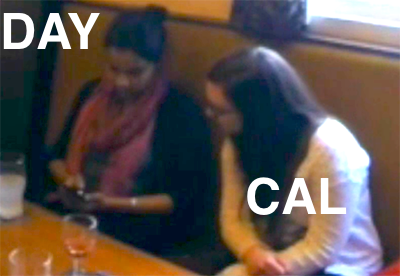
\includegraphics[width=.3\linewidth]{Graphics/3-1-Empirical-Pub/FragmentCollabSearch-2}} \quad
    \subfloat[Rotating the screen to show an email, from \ref{sec:empirical pub findings joke}]
        {\label{fig:discussion embed accountable rotating}%
        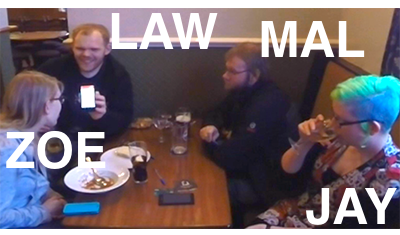
\includegraphics[width=.3\linewidth]{Graphics/3-1-Empirical-Pub/FragmentEmail-4}} \quad
    \subfloat[Sharing screen visibility to show failure of device to respond to voice, from \ref{sec:empirical cafe findings capability}]
        {\label{fig:discussion embed accountable leaning-2}%
        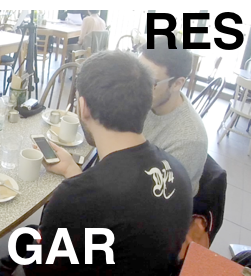
\includegraphics[width=.3\linewidth]{Graphics/3-2-Empirical-Cafe/FragmentMamma-2}}
    \caption{Examples from the first two studies of individuals making device use accountable by sharing visibility of the device screen.}\label{fig:synopsis discussion conduct device-use using accounting}
\end{figure}
\end{revisedsubmission}

\begin{revisedsubmission}
Furthermore, the specifics of input to the \ac{VUI} were hearable to those in earshot, as a result of interaction unfolding through talk to the device.
These requests to the \ac{VUI} device were occasioned in and through the conversation, and as a result of the hearable nature of the request and context within which it unfolds, members' requests are made naturally accountable (i.e. the specifics of the interaction with the \ac{VUI} are reportable as well as hearable).
For example, in the cases presented in \ref{ch:empirical cafe} there were conversations about animal accents, the time of sunset, and the capability of the \acp{VUI}, and each of these conversations established the context within which the \ac{VUI} request was made.
In other words, members' request to the \ac{VUI} was hearable as a result of it being delivered through talk, and reportable as a result of it being occasioned in and through conversation.
However, the responses from the \ac{VUI} typically defaulted to displaying information on the touchscreen of the device.
Members reported these responses either by providing a verbal or visual account of how the \ac{VUI} responded (e.g. showing the screen or verbally explaining the response), or through further \ac{VUI} interaction (i.e. if the device did not respond they would perform further address to the device, through which it is established the prior request `failed`).

%Although hearable to those in earshot, members accounted for their spoken input to the \acp{VUI} in and through the conversation, either before (e.g. as a `preparatory' account) or after the request to the \ac{VUI} was completed, or in response to being \textit{called to account} as a member responded to the device user's utterance to the \ac{VUI} (see \ref{sec:empirical cafe findings answering}).

In the third study, interaction with a \ac{VUI} smartspeaker was done entirely through voice and thus the specifics of their interaction with the device were hearable and made reportable, given that the use of the \ac{VUI} unfolded as part of the ongoing interactional project that occasioned its use (see~\ref{line:naturalaccountability}).
The talk to the \ac{VUI} was hearable through its utterance, and made reportable through its perspicuity to the ongoing activities in the setting (e.g. testing a new device in the home, playing music at a party, or playing a game together while eating dinner).
However, members did provide preparatory accounts in the home in instances where, for example, others were expected to play a game together using the \ac{VUI} (see \ref{sec:empirical home findings game}).
%Often, the hearability of talk to the \ac{VUI} and responses from the \ac{VUI} went some way to establishing the natural accountability of members' interactions with the device by making the specifics of those actions hearable.
In the three fragments of data presented, other members in the setting (i.e. those who were present for the \ac{VUI} use), were ostensibly able to recognise and practically reason about the interaction with the \ac{VUI} device through the requests to and responses from the \ac{VUI}.
This point is exemplified most clearly in instances where the user's request `failed', for example, and members collaborate on addressing the technical troubles with the \ac{VUI} without invitation or detail on the problem by the `original' \ac{VUI} user.
In this sense, the data demonstrates how members accountably recognise the initial request to the \ac{VUI} and the \ac{VUI}'s failure to adequately respond to that request, and practically reason and respond to it by taking further action, either by repeating or rephrasing the request (and, for example, often with different prosody).
In this, members did not explicitly report a failure of their request, as this was done through the use of the device, establishing its use as, perhaps, more `public' in nature.
\end{revisedsubmission}

A final note on this issue is to remark that, of course, members accounting for their device use is directly tied to the cohort and setting within which the device use occurs.
All the studies in this thesis focus on device use when people are with friends and family, and in a casual-social setting.
This links with the prior discussion above with regards to the rules of such a setting by establishing what is acceptable~\citep{Laurier2001}, and furthermore, it establishes the context in which the expectations for how to deal with situations where technology use occurs are managed:
\begin{quote}
    [T]here are many expectations about appropriate engagement with various technologies, including mobile phones---and more specifically texting on mobile phones---that are to do with how those particular cohorts organize their everyday affairs
    \quoteauthor{\citet[p. 262]{Tolmie2008}}
\end{quote}
In this, the practices explicated in this thesis represent and speak to the members of these settings, and this context is imperative to making sense of these findings.


\begin{revisedsubmission}
\paragraph{Collaborating on device use} \hfill \\
Members also included others in their interactional projects as a collaborative activity.
This either relied on \textit{assistance from others} such as guidance on what to search for, spelling (primarily study one), or verbal reports of the specificity of what was being done with the device.
It also relied on \textit{sharing control} of the task by multiple members being involved with the task either on the same device, or different devices~\citep{Brown2015}.

In the case of the first study, members always retained control of the use of their own smartphone by holding it in their hand, although, they did ask others for help with search terms (see \ref{sec:empirical pub findings newinfo}) or for performing requests to the \ac{VUI} if their device did not `understand' their pronunciation (see \ref{sec:empirical cafe findings answering}).
This suggests that the nature of \textit{personal} portable devices such as smartphones supports collaborative practices \textit{through invitation}.
In the second study, another co-present member attempted to complete the task on their own device as someone was struggling to use their \ac{VUI}, \textit{without invitation}.
Moreover, in the third study, featuring only shared \ac{VUI} devices, members self-selected to assist in completing members' interactional projects, again by `taking turns' to use the \ac{VUI} without invitation.

In this regard, interaction through voice, i.e. talk, remains the most obvious way in which members' conduct and use of devices is made recognisable and accountable to others, e.g. as part of the conversation.
With the accountability of device use, co-present members are able to \textit{recognise} and ostensibly self-select, without invitation, to involve themselves in the interactional project.
This led to members answering questions directed at \acp{VUI} (see \ref{sec:empirical cafe findings answering}), assisting with early termination of the \ac{VUI} response (see \ref{sec:empirical home findings music}), or assisting with the initial device user to complete their interactional project (see \ref{sec:empirical home findings game}).

\paragraph{Summary} \hfill \\
This ethnographic study has shown how members were able to interleave their use of devices in conversation to complete their interactional projects.
This rubs up against critiques others have made that suggest the use of---or even the mere presence of---devices in conversation have an isolating effect~\citep{Turkle2011}.
This thesis, through the adoption of an analytical lens that is 1) agnostic to the morals of actions and unaccountable factors, and 2) is used to reveal the accountable situated action of members within the setting, and shows how this interactional work was co-accomplished by members in the setting as \textit{part-and-parcel} of the face-to-face conversation.
In other words, \textit{members accountably attend to interleaving device use in conversation}, and that with the three technologies studied, this use was shown to be collaborative at times.
This collaboration turned upon the specificity of the device use being made observable and reportable\footnote{It was always recognisable to members of the setting that a person was \textit{using} a device, but only the use of a \ac{VUI} intrinsically makes the \textit{specifics} of that use hearable to those in earshot in---and naturally accountable through---its use in conversation.}, and with touchscreen-based interactions this was done through visual or verbal reports.
In the cases of talk to \acp{VUI}, the interaction itself was hearable and through its utterance as a situated action,  and made the specifics of the user's device interaction accountable to the setting as part of the interaction in the setting.
In turn, and any troubles with the technology that users experienced were attended to as matters concerning the occasioned interactional project.%, allowing members to respond to the specifics of the device use.

Through the presentation of empirical data, members' interactions with devices were interleaved amongst the conversation in each setting.
Members did this through occasioning the device in talk or through the conversation occasioning the device use.
They accounted for interactions with the device, engaged others in their device use through questions and requests for assistance, and ostensibly treated interactions with the device as part of the normative moral order within the setting.
The next section turns to discussing a crucial factor in relation to the observations that unfolded: the methodological considerations of this research.
\end{revisedsubmission}



% *********************************************************************************************************************



\section{Methodological considerations}\label{sec:synopsis discussion method}
\begin{revisedsubmission}
The objective of these observational studies was to understand how members practically attend to the matters of using a device in a multi-party conversation.
Accordingly, the analytic orientation of ethnomethodology was adopted.
Crucially, ethnomethodology provides the analytic lens to explicating the members' practical action and practical reasoning~\citep[p. 27]{Crabtree2012} to make sense of and reveal their methodical accomplishments as situated action (see \ref{sec:background approach em sequentiality}).

As the literature review established, this thesis is far from being the first piece of work to adopt an ethnomethodological orientation to studies of everyday life (see \ref{sec:background litreview f2f}), nor is it the first piece of ethnomethodological work to `create' the situation in which the study was to take place (i.e. participants were recruited to go to a setting, rather than the researcher going to a setting in which participants are already assembled).
For example, \citet{Suchman1985}'s work, Plans and Situated Actions, which has profoundly influenced \ac{HCI} and \ac{CSCW}-based studies of interaction, adopted an ``uncontrolled experimentation''~\citep[p. 114]{Suchman1985} approach to studying the use of an agent-based photocopier (see \ref{sec:background litreview f2f turn-to-the-social}).
In her work, although the basis for on participants were using the photocopier was a research study, participants' interactions were unscripted and unguided, or rather, ``uncontrolled''.
This is the overall approach taken with this thesis, insomuch that although participants were recruited to take part in a research study, there was no specific activity or task for participants to do, other than socialising together `as they normally would'.
The participants can assumedly be considered competent for this as they were recruited as families or groups of friends.

Although the analytic perspective adopted in this thesis was uniform across the three studies, the first two consisted of a video-recorded observation for ninety minutes, whereas the third consisted of contextual audio recording in the home over one month.
The study design decisions were based on the appropriateness, or perspicuity, of the device interaction that was of concern to the setting.
This section examines two key aspects that are relevant in terms of the methodological contributions of this thesis, namely the application of this approach in relation to the selection of settings perspicuous to the studies, and of the validity of the methodological choices taken.
\end{revisedsubmission}



% *********************************************************************************************************************



\subsection{Choosing a setting}\label{sec:synopsis discussion method setting}
\begin{revisedsubmission}
The first two studies in this thesis were video-based ethnographic studies.
Participants were recruited for the purpose of socialising as groups of friends who would usually socialise together in either a pub or a caf\'{e}.
This thesis follows in the tradition popularised in the \ac{CSCW} literature of studying the work of a specific setting, such as traffic control rooms~\citep{Bentley1992}.

In reviewing the progression of the development of \ac{HCI} studies, \citet{Grudin1990} remarks that:

\begin{quote}
    [There is] increasing preparation for the next outward step of the interface, into the social or work setting [\ldots] since most work occurs in a social context, computers will support it more successfully if they implicitly or explicitly incorporate social and organizational knowledge.
    \quoteauthor{\citet[p. 264]{Grudin1990}}
\end{quote}
In this, \citet{Grudin1990} provides the rationale for engaging in ethnographic studies of social settings in which technology use would eventually unfold, with ethnomethodology especially suited to this cause given its attention to the members' methodical accomplishments.
Furthermore, \citet{Heath1994} cautiously summarise what they called the ``lack of success of \ac{CSCW} systems'':
\begin{quote}
    [T]he lack of success of \ac{CSCW} systems derives not so much from their technological limitations, but more from their insensitivity to the organisation of work and communication in real work environments.
    \quoteauthor{\citet[p. 155]{Heath1994}}
\end{quote}
This thesis, of course, studies non-work settings, but given the now widespread use of devices in casual-social settings (see~\ref{sec:background litreview society}), there is an established case to undertake studies to reveal the details of the social organisation of interaction in everyday life settings, to support the design of technologies that are used within.
The rise of ubiquitous technologies ratifies the need to study everyday life in which these technologies are used—this is part of the \textit{turn to the social} (see~\ref{sec:background litreview f2f turn-to-the-social}).
\end{revisedsubmission}



% *********************************************************************************************************************



\crpagebreak\subsubsection{Choosing a public casual-social setting for portable device use}\label{sec:synopsis discussion method setting public}
\begin{revisedsubmission}
Ethnographic studies in \ac{CSCW} transgressed on to examining the particulars of everyday life, such as watching television~\citep{Rooksby2015} or families eating together at the dinner table~\citep{Ferdous2016}.
This is the work that this thesis methodologically follows.
A crucial factor that unfolds in all of the prior studies discussed, and that is fundamental to any ethnomethodological study (see~\ref{sec:background approach em comptency}), is the perspicuity of the interaction to that setting.
For example, concerning studies of how couples watch television together and use a mobile phone, it deductively follows to capture data in the main room of the home in which television watching occurs.
Likewise, it follows to examine the use of technology at mealtimes at family dinner tables.
To summarise, the site of the study naturally follows from the activity to be studied.

With this thesis, however, greater justification is given to the selection of settings because such a choice of setting is ostensibly less deductive. With the two video-supported observational studies, two public settings were chosen for the research to take place.
The type of setting was initially conceptually identified as a place where people gather and socialise together.
The settings of a pub and caf\'{e} were then selected for a variety of reasons (see \ref{sec:empirical pub design setting} for justification of a pub and \ref{sec:empirical cafe design setting} for justification of a caf\'{e}).
Summarily, however, there was already literature that revealed the social and relaxed nature of interaction in these settings, and of the device use in these settings.
Moreover, personal experiences of technology being used in these situations further influenced this decision.

The selection of these two settings required pre-negotiating access with business owners to ensure studies were able to take place and to ensure procedures were in place for dealing with inadvertent data collection of members of the public (e.g. people passing through the background).
However, while \citet{Rooksby2013} argues for such studies taking place in a lab-based setting, it was decided that  as there were not factors that needed to be controlled, and as there was no equipment or task other than socialising needed, there were no overriding benefits to running a pseudo-realistic lab-based study over running studies in an 'actual' setting.
Furthermore, obviously, others raise issues with this, remarking that laboratory studies are ``hardly the stuff of ethnomethodology''~\citep[p. 8]{Dourish1998a}, underscoring a need to get as close as possible to the phenomena of interest rather than reliance upon creating a simulated setting.
\end{revisedsubmission}



% *********************************************************************************************************************



\subsubsection{Choosing a home setting for VUI smartspeaker use}\label{sec:synopsis discussion method setting home}
\begin{revisedsubmission}
Given the underlying emphasis to study conversation around the naturalistic use of technology, and to ensure consistency with the first two studies, the third study took place in a setting perspicuous to the use of the device---the home.
Of course, \ac{VUI} smartspeakers were designed for places such as the home, and thus this outcome was straight-forward.
The challenges of studying interaction with new technology are, however, that users may not have competence in operating it.
In some experimental studies of new voice interfaces, for example, researchers have provided training (e.g. \citet{Molnar1996,Schaffer2015}) to ensure users' competency before an experiment with a \ac{VUI}.
The goal in this thesis, however, was to examine the interaction that unfolded around a device, not just with it, or as part of an initial encounter with the technology, or by following training or guidance on how to use the technology.
The goal was to understand how these technologies are used as part of routine interaction in the home. 
Therefore, to get closer to the phenomena of using these home-destined technologies, a more longitudinal approach to the study was necessitated.

As discussed previously within the empirical chapter concerning conversation around the use of \ac{VUI} smartspeakers (see~\ref{sec:empirical home design data}), this study relied upon audio collection only, and upon selective recording rather than continuous recording.
Given the longitudinal nature and the setting in which the study took place, these decisions necessitated careful consideration of how to capture data ethically, sensitively, and practically. Other approaches to studying technology in the home include repeated interview visits (e.g. \citet{Fuentes2019}) and diary studies (e.g. \citet{Forlizzi2007,Jokela2015b}), yet here there was an intent to actually understand the situated action of members that cannot be explicated through such methods.
Furthermore, although some studies of voice interfaces can rely upon self-reported logs of devices (e.g. \citet{Ammari2019}), given the need to examine interaction around the use of the devices this was not a practical method to adopt.
Others adopted methods such as relying on participants to start or stop recording devices before or after the interaction in a space or with a device, as previously done with portable device use during television watching~\citep{Rooksby2015}.
This would be problematic in this study as the use of \acp{VUI} can be started and finished in under a minute without much preparation.
Watching a television programme may consist of being within a specific space for thirty minutes or more, for example.
On the other hand, using a \ac{VUI} may take a matter of seconds with a user simply `passing through'.

Therefore, there was not a practical approach within the existing literature on how to accomplish the data collection for this study respecting the constraints outlined above.
To achieve the goal of this thesis, a specific recording device was designed and created for this purpose (and has since been released as open source software\footnote{See \url{https://github.com/MixedRealityLab/conditional-voice-recorder}}.) to selectively record interactions triggered by nearby users uttering a word.
This recording device (known as the \ac{CVR}) allows a longitudinal study to take place, in which participants learn (or not) how to use the \ac{VUI} within the home without guidance from researchers, in line with the prior two studies' approach of not guiding interaction with devices.
The \ac{CVR} is always `listening'---much like the \ac{VUI} smartspeakers---and retain the last minute of audio in memory.
When the programmed word is spoken, the device saves this prior minute and records for one further minute (extending this recording if the interaction with the device continues).

Furthermore, it allows for fewer data to be collected, to be done so ethically without capturing all matters of home life, and to not rely upon participants to manage their involvement in the study (i.e. members can focus their efforts on their normal mundane activities in the home as opposed to concerning themselves with the data collection).

The audio collected in this study provides a rich insight into the interactions in the home, in much (although not entirely) the same way as video data:
\begin{quote}
    [While video data] can form an archive, a corpus of data that can be subject to a range of analytic interests and theoretical commitments, providing flexible resources for future research and collaboration.
    \quoteauthor{\citet[p. 2]{Heath2010}}
\end{quote}
However, this brings with it a set of limitations, as \citet{Crabtree2012} elaborate:
\begin{quote}
    [Y]ou cannot see what people are doing alongside of the talk and there are circumstances where this may matter. [\ldots] Always be prepared to elaborate with notes the surrounding action that envelops the sequence of talk you are recording.
    \quoteauthor{\citet[p. 82]{Crabtree2012}}
\end{quote}
The approach in this study meant that fieldnotes also could not be taken as data collection was to take place over an extended period without a researcher present.
These two factors mean that this thesis presents only partial records of interaction in the home; however, given the parameters outlined above, and the focus being primarily interaction around the use of the \ac{VUI} device, this was seen as an adequate compromise.
What this situation means is that the data presented in this thesis comes with caveats, such as the inability to comment on conversations relating to the \ac{VUI} device away from the device, or matters that influence the \ac{VUI} use which unfold over a minute before or after interaction with the device.
These caveats limit the drawable conclusions this these can make with regards to commenting on the specific families' use of, and conversations about, different technologies in the home.
However, they do not preclude the examination of how their specific interactions with and around the device unfold \textit{in vivo} where it was recorded.
\end{revisedsubmission}



% *********************************************************************************************************************



\subsection{Methodological validity}\label{sec:synopsis discussion method validity}
\begin{revisedsubmission}
The approach that was taken in this thesis is not laboratory-based given the clear emphasis on selecting settings in which device use unfolded.
In the first two studies, the settings were pre-selected as part of the study design, the participants were all recruited as groups of friends to take part in the study.
In the third study, households were recruited as a family to take part in the study together.
The purpose of each study was described as one in which interactions with and around technology were to be observed.
Such an approach precludes conclusions of matters relating to why device interaction occurred as reasons of motivation, or other non-accountable factors.
These issues were disregarded in any case, given ethnomethodology's orientation to the naturally accountable activities of members only.
Therefore, this thesis' approach to studying the interactional minutiae of members' accomplishment reveals how and for what purpose \textit{in conversation} device use unfolded.

Moreover, in line with existing work in ethnomethodology on the notion of validity, this thesis does not pretend to demonstrate \textit{all the ways} in which \textit{all interactions with and around devices} might unfold.
This is a key tenet of ethnomethodological studies in that, through the presentation of the ethnographic record:
\begin{quote}
    [M]embers can recognise the work of a setting and also, as they are known and used in common, the machineries of interaction that they employ to accomplish and organise that work too.
    \quoteauthor{\citet[pp. 155--169]{Crabtree2012}}
\end{quote}
Thus, it is established that the work of producing the ethnographic report of members' actions is such that members can read and recognise the methods that are explicated.
This is because this record is constructed using the recognisable accountable practices of the members in the setting, rather than theorising about members' actions.
In this sense, this thesis presents the members' practical action and practical reasoning, rather than the analyst's theoretical reasoning.
The reliance upon only examining the accountable actions precludes the production of generalisable statements, but also underwrites the validity of the findings of this thesis.

In summary, this thesis selected settings which were perspicuous to the activity under investigation and recruited friends and families to take part in a research study.
Such an approach precluded discussing motivations for the device use that occurred, however, the analytic orientation of this thesis also precludes such a stance (given its emphasis on revealing the naturally accountable activities of members, rather than assembling a theoretical understanding of their actions).
It is from this regard of producing a record of accountable actions recognisable by members that establishes the validity of the approach taken in this thesis.
\end{revisedsubmission}



% *********************************************************************************************************************



\section{Insights for design work}\label{sec:synopsis discussion design}
\begin{revisedsubmission}[JR-5a, JR-5b, JR-3a, ER-2b, ER-2c, ER-3a, ER-3b, ER-3c, IR-4: Introduce the third discussion point. This is not to designate these points as implications for design but of matters that relate to design literature.]
This chapter's last reflection is upon how interaction unfolded across the three studies with an insight to supporting future design work.
Crucially, this chapter builds upon this thesis' methodological contributions to further examine members' conduct, to identify the collaborative efforts, and how \ac{HCI} and \ac{CSCW} might respond to these efforts.

This section will reflect upon the multi-party device interactions that unfold in each study, how this turns upon the accountability of device use, and how members collaborate as part of their interactional projects.
This will return to the case that the design and use of \acp{VUI} is made naturally accountable such that users can involve themselves in interactions collaboratively without invitation, and that this is of relevance to existing literature in \ac{HCI} to design collaborative systems for collocated interaction.
\end{revisedsubmission}



% *********************************************************************************************************************



\subsection{Collaborative device use}\label{sec:synopsis discussion design collab}
Previously, this thesis introduced work in \textit{mobile collocated interactions} \iresubmission{and \ac{HCI}}  which focused on the notion that device ownership will, in the future, occur with \textit{shared} devices, and that these devices will support \textit{multi-user} interactions that are \textit{collaborative}~\citep[see~\ref{sec:background litreview design mobilehci}]{Lucero2010d}.
Indeed, the findings of the empirical chapters in this thesis show that, in each of the studies and with each modality of interaction with a device, \iresubmission{members engaged in collaborative device use.}
\iresubmission{For example, with touchscreen interaction, members were observed collaborating, with one member  providing the query terms for a mobile search to be completed by another as part of the interactional project occasioned by their conversation (see~\ref{sec:empirical pub findings newinfo}).
In another case, one member proposed a rephrased request to the user of a \ac{VUI}, given that the members practically reason that the device `misinterpreted' the prior request (see~\ref{sec:empirical cafe findings newinfo}).
In a third case, the members of a setting took turns trying to start a game by issuing new requests to the \ac{VUI}, varying the prosody and words used in response to the failures of prior requests (see~\ref{sec:empirical home findings game}).}
This first case, for example, augments the existing literature that identified collaborative mobile search as an everyday task.
This examination by \citet{Brown2015} identified that there was
\begin{quote}
    [\ldots] considerable attention, effort and thought given to co-conversationalists while using a mobile device. Rather than shutting off conversationalists from each other, the devices become a site of investigation and discussion.
    \quoteauthor{\citet[p. 516]{Brown2015}}
\end{quote}
\iresubmission{This thesis extends this finding to encompass mobile device use for other purposes too, and how such practices unfold with both touchscreen device use and \ac{VUI} use, and that members bring this use into conversation in a casual-social setting.}
%This work provides numerous exhibits of multiple people collaborating to search for information using a mobile device in everyday life --- the interactionists studied may be occasioned by one member, but often multiple people are brought into the interaction through the embedding practices discussed above (see~\ref{sec:empirical pub discussion coop}).

Portable devices such as smartphones are inherently personal in their design and use~\citep{Lucero2010}, engendering `private' use \iresubmission{whereby even if co-present others are aware of---and can observe---device use unfolding, they often cannot observe or report on the \textit{specifics} of that use (e.g. they might not have a line of sight).
This is due, in part, to the relatively small size of device screens which inhibit greater visibility of the screen by those who are present beside the user.
Attempts to disrupt this private nature of device use have included adding large screens to settings to encourage users to share content from devices~\citep{Lucero2012}.}
However, the findings from the first study show how \iresubmission{devices are used as part of collaborative efforts by members, by the user asking others for assistance in completing their interactional projects, irrespective of the small size of the screen, or by making the screen visible to others.}
As they did this, they \iresubmission{made the device interaction accountable to others the setting, revealing the specifics of what was being done with the device, and thus transformed the `private' device use to one where the specifics of that device use were observable to \textit{some} others (i.e. this was not `public' use, however, as the screen may have been made visible only one other member).}

\begin{revisedsubmission}
%As discussed above, through conversation, members accounted for their interaction with their touchscreen devices (see \ref{sec:synopsis discussion conduct device-use using}).
Following the reflection of the findings from the first study, this thesis posed the question of how the practices of device use could unfold when the interaction mode was augmented with voice input (see~\ref{sec:empirical pub summary}), given that in such cases the talk to the \ac{VUI} would be hearable to those in earshot, making the specifics of users' actions hearable.
In particular, this outlook asked how members would use a \ac{VUI} as part of a gathering in a casual-social setting (see~\ref{sec:empirical pub summary outlook}).
As \citet{Crabtree2012} remark:
\begin{quote}
    [T]alk is the most obvious and pervasive way in which members conduct their work and make whatever it is that they are doing into an intersubjectively recognisable and naturally accountable activity.
    \quoteauthor{\citet[p. 44]{Crabtree2012}}%[p. 44]
\end{quote}
\end{revisedsubmission}
The second study addressed this matter and revealed how members' talk to devices, as interleaved within conversation, \iresubmission{made the specifics of their actions reportable, with the performance of the request organised within the organisation of the conversation in which the device use was occasioned}.
Additionally, this study brought to the fore that by switching the interaction mode of the device to voice as well as the use of the touchscreen, members ostensibly \textit{self-selected} to involve themselves with ongoing device tasks.
For example, they chose to perform requests on their own device if another member was struggling (see \ref{sec:empirical cafe findings newinfo}), or they offered assistance to the member to help diagnose problems (see \ref{sec:empirical cafe findings answering}).
\iresubmission{In this sense, device users did not necessarily account for the specifics of their device use, because their specific input to the device was hearable and made accountable through coherence with the ongoing conversation in the setting.
The action of uttering a request to the \ac{VUI}, in turn, was shown to occasion other members' self-selecting to respond to the device user's request (in other words, talk to the device was responded to by other people who were not the recipient of the utterance).
However, members provided accounts, especially to provide the details of the response from the \ac{VUI}.
At times these accounts were implicit made by members (i.e. when a member uttered a subsequent identical request, through which they establish the failure of the previous request).
At other moments, it included members explicitly confirming the success or failure of the \ac{VUI} to respond to the request.
In this, through the utterance of the request, the device interaction with the technology becomes `semi-public', insomuch that members' requests to the \ac{VUI} were made naturally accountable through their use as part of the social interaction in the setting, yet members were relied upon by others for verbal or visual reports of the \ac{VUI}'s responses given that these responses were displayed on the device touchscreen.}

%These findings showed how completion of the task was, in a sense, \textit{democratised}, by the switch to voice interaction, as the control of the completion of the task was removed from the device user and became managed through the conversation and social order of the setting (see~\ref{sec:empirical cafe discussion multiparty}).
%However, although the completion of the task was democratised, members still retained some control over interactions---they were relied upon the user(s) to report messages displayed on the screen, or to read information that had been found, for example.


The third study moved this examination into the realm of interaction through voice only, and where the technology under study became a shared device in the home.
As such, although the observations in the study of \acp{VUI} on portable devices explicated the hearable nature of the request made to the \ac{VUI}, and its coherence to the conversation establishing its natural accountability, in the study of voice-only interactions, the findings reveal how all members of the setting could orient to and attend to matters of the device interaction.
The hearable nature of requests was again revealed, with members' requests being explicitly held to the normative moral order by those in the setting (see \ref{sec:empirical home findings music}).

\iresubmission{Furthermore, with these interactions, the response was hearable, \textit{and reportable} through the coherence of the accountable request and ongoing conversation in the setting that occasioned the original request.
This natural accountability of the response, and the shared and public nature of \ac{VUI} smartspeaker in contrast to a portable smartphone, has the further consequence that all co-present members can not only respond to the request, but can also respond to the response from the \ac{VUI}.
This was seen as members respond to the \ac{VUI}'s response and make successive requests in accord with the prior one, e.g. in ratcheting up the testing of the \ac{VUI} (see~\ref{sec:empirical home findings capability}), or as members take turns attempting to start a Skill  (see~\ref{sec:empirical home findings game}).
In these cases, no member could retain control over the device and the `politics of control'~\citep{Porcheron2018} were managed through the social order of the home\iresubmission{, as part of interaction in the home between those who are present.
In some cases, members were called to account for interaction with the device that another member deemed out of place for the setting (see~\ref{sec:empirical home findings music}), but in this situation, it was not the purpose of the device interaction at hand, but the use of language involved that was remarked upon as being deemed problematic.
What the data in this thesis shows is that the use of a \ac{VUI} smartspeaker, as occasioned by conversation, unfolds as a `public' activity, whereby the specifics of that use are hearable and reportable to those who are co-present.
The data shows crucially how this use is regulated through the social order of the home as an accomplishment of the members in the home.}

\begin{revisedsubmission}
Through the careful reflection on members' conduct and how they accomplished their collaborative efforts to complete the occasioned interactional projects, this section has identified collaborative action amongst members in such settings, and this establishes the case for further studies in \ac{CSCW} to critically examine the nature of studying interaction in such settings.
Some literature has examined this (as discussed above, see~\ref{sec:synopsis discussion conduct}), but crucially, what this thesis shows is how there is further cause to examine such settings to reveal the collaborative efforts within, to support design work.
Although the definition of a casual-social setting was broad, as a concept it builds upon the work of others who have called for ethnographic studies of social settings~\citep{Grudin1990}.
The need to study the organisation of interaction of settings in which technology is to be used collaboratively is well rehearsed (e.g. \citet{Crabtree2009,Heath1994}), yet the work in this thesis suggests that such technology was shown to be deficient in meeting members' needs, e.g. multiple interactional projects were left unresolved. %\footnote{Of course, this thesis argues that the non-resolution of prior conversational topics is part of interacting in a casual-social setting, yet this thesis still proposes that technology \textit{could} meet these needs such that members need not abandon an interactional project.}.
Nevertheless, as this thesis has argued, members undertake interactional work to account for and accomplish this collaborative effort and the `need' to `successfully' complete an interactional project ostensibly does not exist in a casual-social interaction, therefore \ac{CSCW} should take the opportunity to identify ways to ameliorate these challenges through further ethnographic work.
The concept of a \textit{casual-social setting} is established around the notion of members' conduct, and this thesis has unpacked three such studies of that.
Members' conduct is, of course, cohort dependant (see~\ref{sec:synopsis discussion conduct device-use using}) and thus, further studies are needed to reveal more about the interactional projects, and ways in which members' problems are addressed with technology.
The next section further reflects upon these responses from the \ac{VUI} and how the collaboration that unfolded turns upon them.
\end{revisedsubmission}



% *********************************************************************************************************************



\subsection{VUI responses as supporting further action}\label{sec:synopsis discussion design vuiresponses}
\begin{revisedsubmission}
This final discussion section examines an area of concern for \ac{HCI} in the challenge of designing interfaces to support collaborative action amongst members of the setting.
Collaboration, as discussed above, unfolded as an interactional accomplishment in each setting, as members worked together to complete their occasioned projects.
With the latter two studies, however, this collaboration ostensibly turned upon the hearable nature of the interaction with the device.
This section critically examines how this interaction could be further examined, linking to existing publications in \ac{HCI}, to design interactions that meet members' interactional needs.

In reflecting upon the study of \ac{VUI} smartspeakers in the home, \ac{VUI} interaction is shown to consist of the form \textit{request to \ac{VUI}-response from \ac{VUI}}.
At times, and in all the cases of \ac{VUI} device in the home presented in this thesis, a response from the \ac{VUI} is followed by successive requests by the members of the setting.
Through the analysis, the \ac{VUI} responses themselves are analysed by members for the `account' of sorts they provide on the state of the \ac{VUI} device, and its processing of the previously made request, i.e. the response (or not) of a failed request occasioned members to practically reason and perform further actions to accomplish the interactional project.
The data from both studies two and three suggest a level of inadequacy of some responses \textit{as resources} to furnish this analysis to proceed with the interaction.
Consider how members in the third study fail to start the Beat the Intro Skill due to the repeated non-obvious source of technical trouble (see~\ref{sec:empirical home findings game}) before the device ultimately provides a response to a request that includes a partial transcription of the user's spoken words, and the \ac{VUI} offers a next candidate action.
This action provides a mechanism to practically reason about the processing of the voice-only device.
Of course, with touchscreen-based devices, this mechanism for users to reason about \ac{VUI} troubles was provided through messages displayed on the touchscreen, but these were only known to others if the device user `made them available' by reporting them (verbally or visually).

This thesis argues that the accountable nature of a `verbal' response from a \ac{VUI} smartspeaker is used as a resource by the original \ac{VUI} user, and other co-present members, to make successive requests.
It is through the natural accountability of members' successive requests to the \ac{VUI}, and how these turn upon the response from the \ac{VUI}, that reveals the practical reasoning of multiple members, collaborating to complete the interactional project.
Members demonstrably show reasoning about failure through a discussion in conversation (see~\ref{sec:empirical cafe findings newinfo}), or through repeated utterances to the device by different members with different prosody (see~\ref{sec:empirical home findings game}).
In both cases, it was this natural accountability of the response, established through the ongoing work of the setting, that provided the resource for further action.
\citet[p. 10]{Porcheron2018} term this characterisation of responses as ``resources for further interaction''.
In examining interaction in a multi-party setting, this resource is established as supporting further interaction by  members of that setting to complete the interactional project.

Designers might, then, consider how members attending to technical troubles with the \ac{VUI} are also attempting to practically reason about the source of trouble, be it a system problem or a transcription problem.
The response (or no-response) is treated as an indicator of what this trouble is.
With the \ac{GUI} on smartphones, the \ac{VUI} displays text to `explain' the processing of the user's request, and with screenless devices, this is done through the verbal response (or lack thereof).
At times, the \ac{VUI} provided a reference to the next candidate action of the device, or the transcription it generated of the user's spoken words, and what provisionally might or might not happen next (see~\ref{sec:empirical home findings music} or \ref{sec:empirical home findings game}).
\citet{Porcheron2018} remark how, adjusting, or `designing' these responses to display this processing, would provide users with resources that can support and occasion further interaction with the \ac{VUI} device.

In summary, with \acp{VUI}, the specific request was shown to be made an accountable accomplishment through the conversation in which it was interleaved~\citep{Porcheron2017}, and with \ac{VUI} smartspeakers, the hearable response from the \ac{VUI} was made accountable through both conversation and the request which triggered it.
In returning to consider this development in terms of the mobile collocated interactions literature, this thesis remarks upon how the use of the \ac{VUI} as occasioned in conversation accounts for specific features of device use grossly observable and reportable through talk to all those in earshot.
Much of the design-focused literature in mobile collocated interactions has focused on creating technologies for collaborative use between collocated people (e.g. \citet{Lucero2010d} use mobile devices for brainstorming) using touchscreen technologies.
One such opportunity might be the inclusion of a voice-interface in the design of such systems to transfer interactions with devices to a more `public' sphere.
The notion that voice-based interfaces could be designed to support collaborative interactions between co-present others has been used in some design efforts in \ac{CSCW}~\citep{Jones2012}.
However, through the presentation of empirical data, this thesis reinforces and validates the notion that the adoption of a voice-based interface has the propensity to allow members to collaboratively complete interactional projects occasioned in conversation.
However, through the analytic orientation of ethnomethodology, this thesis also reveals how it is \textit{not enough} to produce a \ac{VUI} to ensure collaborative activity between members---collaboration in these settings turns upon both the practical work of members to make activities accountable, and of the resources the \ac{VUI} provides to users, supporting those who are co-present to take further action in completing their interactional projects.
This thesis stops short of offering implications for what constitutes `ideal' interactions with a \ac{VUI}, but the notion of designing \acp{VUI} for collaborative action should now be perused as an avenue in future \ac{HCI} work, extending prior efforts on collaborative mobile systems (see~\ref{sec:background litreview design mobilehci}).
\end{revisedsubmission}



% *********************************************************************************************************************



\section{Summary}\label{sec:synopsis discussion summary}
\begin{revisedsubmission}
This discussion brought together the main strands of this thesis in order to answer the aims and research questions posed.
It discussed the conceptual nature of casual-social settings, how conversations unfold in such settings, and how device use is accountably and interactionally organised in and through conversation (see~\ref{sec:synopsis discussion conduct}).
By bringing together the methodical accomplishments of members in using devices in interaction, this chapter demonstrates how devices are used as part of socialising together in a group and for the purposes of addressing the members'
 problems occasioned in conversation.
Members also used devices for other purposes, and naturally accounted for this as part of the conversation (e.g. to make jokes, or play games together, and so on).
%This chapter purposefully avoided making generalisable statements, however what it did do, by virtue of the empirical data presented in this thesis, is synthesise how technology is used in interaction, \textit{as part of} that interaction.

The chapter then progressed onto making a number of methodological considerations (see~\ref{sec:synopsis discussion method}), by reflecting upon the ethnomethodological perspective and practical approach taken in this thesis to the three studies.
Each study in this thesis selected a setting that was established as appropriate for the specific technology under examination.
This, combined with the careful approach to explicating members' naturally accountable actions, underscored the validity of the approach taken in this thesis.
This thesis produced thick descriptions of members' actions, and through the recognisability of these methodical accomplishments, this validity is established.

Finally, this chapter turned to discus elements of the collaborative interaction that unfolded within the data (see \ref{sec:synopsis discussion design}).
These instances were identified as turning upon the accountability of device use, with the requests to (and from) the \acp{VUI} making the specifics of the interaction hearable and reportable through the work of the setting.
The collaborative efforts of members were also identified specifically as an accomplishment of members' efforts in the setting through their use of the device.
By considering the existing literature on designing collaborative software for use with portable devices, this thesis posits that the use of a \ac{VUI} has the potential to support collaboration on members' interactional projects in such settings.
Crucially, however, this thesis shows how this requires careful design work through considering the specifics of these requests: it is not enough to just introduce a \ac{VUI} to a setting, one must undertake work---which is beyond the scope of this thesis---to consider how requests to and responses from the \ac{VUI} may be used to accomplish members' interactional projects in a casual-social setting.
\end{revisedsubmission}



%!TEX root = ../PhDThesis.tex



% *********************************************************************************************************************
\chapter{Conclusions}\label{ch:synopsis conclusions}
% *********************************************************************************************************************



\begin{revisedsubmission}
This chapter summarises and brings together the conclusions of the machinery of members' conduct in using a device in and around conversation in a casual-social setting, the collaborative nature of this device use, and the methodological contributions of this thesis.
Finally, this chapter concludes with a summary of the potential future work that could follow on from this thesis.
\end{revisedsubmission}



% *********************************************************************************************************************



\section{Summary}\label{sec:synopsis conclusions summary}
This thesis made a case for studying device use in conversation (see \ref{sec:intro probdef}), adopting a practical approach that eschewed judgements on the values of device use and instead focused on the practical accomplishment of how devices are used during multi-party gatherings in casual-social settings.
\iresubmission*[ER-B: Remove unnecessary narrative regarding good/bad device use]{This case was motivated by a paucity of data on how and for what purpose devices are used in such settings, against a backdrop of existing literature that characterised such use as problematic.}
\iresubmission*[JR-1, JR-3a, ER-1, IR-2: Remove sections discussing and reflecting upon findings related to attention literature and references to EMCA]{The research in this thesis was fundamentally interdisciplinary in its approach and drew upon existing work in Mobile \acf{HCI}, ethnomethodology, and \acf{CSCW}.}

\begin{revisedsubmission}
Through the analytic lens of ethnomethodology, this thesis explicated both the problems that occasioned device use in and through the ongoing multi-party conversation, and how members brought their devices into a conversation to address these problems.
These problems form the foundation for the interactional projects---ranging from information deficits through to desires to play games---occasioning the use of the device as an activity that unfolds within the setting.

This thesis consisted of three studies, each with a focus on the social organisation of groups of people socialising together and making use of a particular technology.
The first study examined conversation around the use of touchscreen portable devices such as smartphones, the second studied conversation around the use of the \acf{VUI} on touchscreen portable devices, and the third studied conversation around the use of screenless \ac{VUI} devices, marketed as smartspeakers.
Each set of studies took place in a specific setting: the first was in a pub, the second in a caf\'{e}, and the third in participants' home, all of which were considered to be `casual-social'.

Through explicating the members' methods of using a device in conversation in these settings, this thesis shows how members accountably organise this use and take part in collaborative activities to complete these interactional projects.
This collaboration was identified as turning upon the natural accountability of device use, which members accomplished through making the specifics of their use visible and reporting upon it in interaction.
When device use was done using a \ac{VUI}, the use itself was made naturally accountable through the talk to the device interleaved amongst the conversation that occasioned it.
In the case of \acp{VUI} that feature no \acf{GUI} (i.e. the smartspeakers), the responses from the device were oriented in the conversations, with members demonstrably attending to---and substantiating the natural accountability of---these responses through the coherence of the initial request and ongoing conversation.
Through the examination and reflection of the data presented in this thesis, the discussed has illuminated how members ostensibly treat the use of devices perspicuously.
Furthermore, it was identified how such device use, rather from detracting from the ongoing conversation, became embedded within the activity of socialising together.
In this sense, the device use did not unfold instead of---or `isolated' from---the social activity, but was performed as an activity within the work of socialising together as a group in a casual-social setting.

These studies inform and further encourage \ac{HCI} work to examine ways of creating technologies to support collaboration on portable and readily-available technologies while people are socialising in groups.
Crucially, by demonstrating the intricate ways in which members accomplish collaborative action to complete interactional projects, drawing upon the resources provided by the \ac{VUI}, this thesis identifies a topic for further examination within both \ac{HCI} and \ac{CSCW}.
Secondly, by exploring members' collaborative actions, this thesis remarks upon moments of when interaction was undertaken with a \ac{VUI} smartspeaker, it was the \ac{VUI}'s responses that reported upon the success---or not---of requests made to the device.
This identified a key concept to consider for future work, reinforcing findings published as a result of the research in this thesis (see \citet{Porcheron2018}), that classify the responses from \acp{VUI} as \textit{resources} for further action as members' problems are addressed.
\end{revisedsubmission}



% *********************************************************************************************************************



\section{Contributions and key conclusions}\label{sec:synopsis conclusions contribs}
This thesis makes three key contributions, corresponding to the research questions posed in \ref{sec:intro rqs}:

\begin{revisedsubmission}
\begin{enumerate}
    \item Explication of the \textit{members' methodical accomplishments} of using a device in casual-social gatherings, detailing how they bring devices into an everyday multi-party conversation, and offering an insight into the differences of how device use is used to address the members' problems that arise in such settings,

    \item Development of the \textit{methodological approach} in this thesis, both in terms of the application of ethnomethodology and of the nature in which \textit{these technologies} were studied \textit{in these settings}, and

    \item \textit{Conceptual insights} of \icorrection{the nature of studies in casual-social settings and `device talk' to \acp{VUI}}.
\end{enumerate}
\end{revisedsubmission}

\noindent These contributions are summarised in the following sections.



% *********************************************************************************************************************



\subsection{Members' methodical accomplishments}\label{sec:synopsis conclusions machinery}
The methodological approach taken with this thesis included capturing `real-world' empirical data of groups of friends or family conversing in a casual-social setting.
\iresubmission{This thesis defined the conceptual choice of setting as one in which friends and family gather to socialise and relax.}
Through the analysis of the captured data, the empirical chapters in this thesis progressively explicated the accountable practices of the members of each setting as they \iresubmission{interleaved} their device use in and through conversation.
The orientation to accountable actions of members in the setting allowed for the formation of thick descriptions that detailed the interactional methods people employed as they attended to the interactional projects for which device use was occasioned.

\iresubmission{Each study identified members' methodical accomplishments that revealed exactly \textit{how} members of the setting brought a device into the ongoing conversation.}
These were brought together in the discussion to reveal how the overall accomplishment of using the three different technologies in conversation is done (see \ref{sec:synopsis discussion conduct device-use}).
\iresubmission{Crucially, the findings reveal how, through using a device in conversation, the natural accountability of members' actions is accomplished as an outcome.
With touchscreen devices, the interactional work to account for device use was done through methods such as articulating what was being done with the device, or making the device screen visible to others.
In cases where the interaction was with a \ac{VUI}, the interaction with the \ac{VUI} (i.e. the \textit{talk to the device}) typically made the specific nature of a member's device use both observable and reportable within the context of conversation within which it was occasioned.
Nevertheless, members accounted for this use by providing further information on what occasioned their use through talk (e.g. they recalled a recent news story), or by providing preparatory accounts for what the interactional project they were about to undertake concerned.
This accountability provided the resources for other collocated members to ostensibly self-select to become involved in the interactional projects, and in turn, at situations where members had technical trouble, collaborate with the device interaction.
In the case of \acp{VUI} on portable devices such as smartphones, in contrast to standalone smartspeakers, the response from the \ac{VUI} was typically returned via the built-in touchscreen.
Through using a device in these settings, members made this response accountable by sharing visibility of the screen, providing verbal reports of responses from the \ac{VUI}, or through further interactions with the \ac{VUI} (e.g. repeating a request), which recognisably establish the case for members reasoning that the device failed to respond to a prior request.}

\begin{revisedsubmission}
Through these three studies, the notion that device use is a mundane phenomenon in the settings is established.
Members' problems, established through the conversation of the setting, occasioned the use of technology---ranging from instances of using a device to find new information in the conversation through to playing a game together---such that the use of the device was \textit{part of} the multi-activity in the setting.
Conversation topics were also brought about as a result of device use, with members introducing an email to the conversation to make a joke, through to projects such as testing the functionality of the \ac{VUI}.
In these instances, again, device use was occurrent alongside---or interleaved with talk---and was brought into the activity of socialising as an ostensibly mundane activity within the setting.
Therefore, this thesis concludes that device use is fundamentally \textit{embedded} in the activity of socialising in a casual-social setting.

Furthermore, as a result of the naturally accountable nature of interacting with a device, dealing with technical troubles and issues in completing device tasks were shown to unfold as collaborative activities.
In this regard, members collaborated on mobile search tasks using touchscreen devices, attempted to find new information with \acp{VUI} on smartphones, and attempted to start games using \ac{VUI} smartspeakers in the home.
In both of the studies involving \acp{VUI}, this collaborative practice unfolded whereby co-present others involved themselves in others' device use \textit{without invitation} or a request for assistance.
This was revealed to turn upon the natural accountability of the use of the \ac{VUI}, which made the specifics of the interaction hearable and reportable within the context of which the use was occasioned.

%\correction{Remove summary of the summary}
% In summary, there are three contributions arising from the machinery members' conduct in a casual-social setting:
% \begin{itemize}
%     \item Device use was occasioned in and through conversation as part and parcel of socialising in a casual-social setting,
%     \item The hearable nature of talk to the \ac{VUI} was made naturally accountable through the use of the device, as occasioned in and through the ongoing conversation, and
%     \item Technical troubles arising from device use were attended to collaboratively, and where the specifics of the interaction were made accountable, members self-selected to involve themselves in these interactional projects.
% \end{itemize}
\end{revisedsubmission}

\begin{corrections}[Clarify the substantive contributions]
Crucially, this thesis challenges existing notions in socio-technical studies that the use of portable devices in such settings is a distraction from ongoing socialising (see \ref{sec:background litreview society together}).
Specifically, this thesis' findings implicate a call for reconsidering how device use is articulated in publications: rather than treat it as incongruous or distinct from social interaction, this thesis emphasises a call for analytic orientations which regard it as accomplished  \textit{in and through} members' efforts to socialise.
Even more pointedly, the findings suggest that device use is part of the \textit{social order} in these settings (see \ref{sec:background approach em work}).
This does not invalidate prior findings by others, as such findings were perhaps indicative of the time in which portable devices were more nascent, compared with the ubiquity of device ownership at the time of these studies (see discussion of device ownership in \ref{sec:intro devices}).
In retrospect, for example, Turkle's more recent calls to `reclaim conversation'~\citep[see p. \pageref{line:reclaimingconv}]{Turkle2015} implicates as much: the work of conversing in these sorts of settings \textit{has changed} as a result of technology use, which now ostensibly permeates it.
However, to regard this change as negative or positive---which is a categorisation based upon morals---is something this thesis intentionally does not speak to.

Secondly, this thesis' work on voice interfaces---both mobile and in the form of smartspeakers---took place as the technologies were coming to mass-market.
Literature that examines their use \textit{in vivo} was nascent and thus this thesis contributes the first empirical account of making such technologies at home.
However, studies of other activities in the making of technology at home bare analogous methods to the use of the smartspeaker.
For example, in the same regard that \textit{multi-screening} became embedded in the work of \textit{leisure time} through sitting on a sofa in front of a television while making use of mobile devices to augment television watching~\citep{Rooksby2015} (see \ref{sec:background litreview society utopia}), smartspeaker devices were placed in \textit{activity centres} in the home---such as the living room or a kitchen/diner---and members made the use of the smartspeaker naturally accountable as part of the interactions in those settings (see p. \pageref{line:activitycentres}).

Finally, the technologies under study in this thesis could still be considered to be single-user---even smartspeakers, which operate on a one-at-a-time person-agnostic operation.
However, research in \textit{mobile collocated interactions} has attempted to address this by exploring ideas for how to embody notions of groupware from \ac{CSCW} in portable devices to support collaboration (see p. \pageref{line:singleuser}).
This thesis specifically contributes the notion of how users' interactions with voice interfaces are transformed into multi-user experiences \textit{by users} through interaction in spite of a lack of specific design cues.
Members does this by accounting for device use and occasioning the device use in conversation.
This was demonstrable in this thesis in many cases, but of note are also situations in which technical troubles with devices were collaboratively dealt with through conversation, especially with \acp{VUI}.
For example, the resources made available through interaction with a smartspeaker---the hearable input and output---facilitate the collaborative actions of collocated users.
The ambitions of the research agenda to design portable technologies for collaborative action could be extended by further exploring the use of voice interfaces, with the findings of this thesis demonstrating the potential of such technologies.
\end{corrections}



% *********************************************************************************************************************



\subsection{Methodological approach}\label{sec:synopsis conclusions method}
\begin{revisedsubmission}
This thesis adopted the methodological perspective of ethnomethodology (see \autoref{ch:background approach}) to unpack members' actions in the settings.
The first two studies took place in the semi-public settings of a pub and caf\'{e}, with participants recruited for the purpose of socialising together, and to be recorded for their interactions.
Participants were informed that the focus of the study was on the behaviours around the use of devices, but that there was no requirement to use any device during the study.
In the case of the second study, participants were asked to use the \ac{VUI} on their smartphone instead of typing where possible, but were again told that this was not a requirement and that the use of the device itself was not required for the study.
These settings were selected as they were perspicuous in regards to the technology being studied, i.e. existing literature and personal experience had already established that technology use unfolds within pubs and caf\'{e} among groups of people socialising.

These two studies were, in some regards, an ``uncontrolled experiment''~\citep[p. 114]{Suchman1985} of sorts, in which people were in the setting for the purposes of being participants in a research study, but that the focus of that study was not on the completion of a specific task or following a protocol.
The researcher was present and socialised with the participants for all the gatherings in these two studies and followed a participant-observer approach throughout the gatherings.
The gatherings took between 60 and 90 minutes, with the study ending at an agreed time with the participants---the uncontrolled nature of the study was such that the study ended where it was ostensibly deemed appropriate by the researcher.
In these two studies, data were collected by video recording the study using fixed wide-angle cameras on tripods, audio recording using a voice recorder, and writing of fieldnotes after the study.

The third study took place in participants' homes and was longitudinal in approach, taking place over one month.
Homes were selected as the site of study because these were the sorts of places that \ac{VUI} smartspeakers were designed for---they are typically non-portable devices designed for use in homes or offices.
A longitudinal approach was also adopted in this study given the recentness of the technology being introduced to market (i.e. less than one month on the UK), with the focus on the study being how the technology was used in everyday multi-party gatherings.
In this regard, each participating household installed the smartspeaker in a communal area of the home.
For data collection, audio capture was selected given the ethical and technical concerns of collecting data in the home (i.e. participant uneasiness about recording video in the home, and the vast amounts of video data that would be generated).
However, a further issue was that it would still remain problematic to continuously record audio in the home (e.g. necessitating an analysis that would be an insurmountable challenge in terms of the length of captured data).
Therefore, an audio recording device was designed and built for this study that captured a minute before and after interactions with the \ac{VUI} only, allowing researchers to make sense of the context within which the device was used (this was called the \acf{CVR}, see \ref{sec:empirical cafe design data cvr}).

Across all three studies, the same analytic orientation was adopted in unpacking the collected data.
Each study adopted an iterative approach, in line with documented practices in ethnomethodology (e.g. \citet{Crabtree2012,Heath2010}), to explicate members' interactional projects, and how they practically interleaved device use within conversation.
Ethnomethodology's focus on the naturally accountable practices of members allows this analysis to present `what is done in the doing', and consequentially support this thesis' underlying goal to reveal how devices are used in multi-party conversation in a casual-social setting.

%\correction{Remove summary of the summary}
% In summary, there are three contributions arising from detailing the members' problems that occasion device use and the machinery of how devices were actually used in a casual-social setting:
% \begin{itemize}
%     \item Recruiting groups of participants to socialise as a group provided rich empirical data to allow for the explication of how technology is accountably used in casual-social settings,
%     \item Selective recording using a purpose-built \ac{CVR} is an effective way of capturing data from a longitudinal study in the home, and
%     \item The ethnomethodological approach taken in this thesis' work has resulted in thick descriptions that report members' naturally accountable actions, and provides the commodity to make sense of and reveal the nature of using technology in a casual-social setting.
% \end{itemize}
\end{revisedsubmission}

\begin{corrections}[Clarify the methodological contributions]
This thesis' contribution in the form of the \ac{CVR} provisions a data capture tool to longitudinally study interaction with a voice-driven technology in the home (see \ref{sec:empirical cafe design data cvr} for the design of the recorder).
Approaches previously adopted to studying technologies in the home include auto-ethnographies, ethnographies, diary studies, log analysis, and interview studies (see p. \pageref{line:prevhomestudy}), with each providing researchers with different levels of insight into the situated use of technology.
This thesis' work in the home is congruent with existing ethnographic approaches and ideas from \ac{CSCW} of placing research technologies in the home~\citep{Tolmie2008a}.
As elaborated on by \citet{Crabtree2003}, the challenge for designing technologies for the home is ``how people live in the home, what they do when they are at home, and the potential role of technologies within the milieu of domestic activities''~\citep{Crabtree2003}; through its selective capture of interaction and the preceding/succeeding use, the \ac{CVR} allows researchers to elicit such an insight with relative ease.

By building and deploying a technology to automatically selectively capture interaction with a smartspeaker over an extended period of time that incorporated ethical considerations of long-term data capture in a personal space, this thesis supports an ethnomethodological analysis by providing rich data that includes elements of the context of interaction.
Other approaches, such as having a fieldworker `on site', can become impractical when studying interaction for extended periods of time, with proposed solutions including asking participants to record their interaction (e.g. \citet{Rooksby2015}).
Alternatives include continuous video capture, as done by \citet{Heath1991} in their study in workplace collaboration, but such work was undertaken among colleagues and under a vastly different regulatory environment.
This thesis took an automated approach that allowed for the collection of data with some semblance of context through the inclusion of data around device interaction.

The richness of the resulting data included in this thesis validates the approach for further studies of ubiquitous computing in the home, and perhaps other sensitive locations such as the workplace.
Such approaches need not be restricted to voice interfaces, but could include other technologies too, detected through properties such as increased electricity consumption.
As ubiquitous computing research continues to examine the \acf{IoT}\footnote{An umbrella term for the routine integration of Internet connectivity to everyday technologies, including sensors and home fittings.}, approaches such as the automated data capture in this thesis are likely to become of even greater benefit.
\ac{IoT} technologies are increasingly incorporating elements of autonomy and portability~\citep{Fuentes2019a,Porcheron2015}, raising challenges for the study of their use: understanding just how people deal with this autonomy in the home will be critical to ensuring systems meet the needs of users~\citep{Crabtree2003}.
%Other research technologies could incorporate selective data capture, or augment existing `\ac{IoT} data hub' concepts (e.g \citet{Crabtree2018}) to support examination of \ac{IoT} use \textit{in vivo}.
\end{corrections}



% *********************************************************************************************************************



\subsection{Conceptual insights}\label{sec:synopsis conclusions concept}
\begin{revisedsubmission}
The final point to address is conceptual insights arising from this thesis.
The insights contribute to existing ideas and work in both \ac{HCI} and \ac{CSCW}.
There are two key concepts this thesis \icorrection{focuses on: the concept of the activity-based settings, and the concept of `conversation' with a \ac{VUI}}.
\end{revisedsubmission}

\begin{corrections}[Refocus the conceptual contributions]
\subsubsection{Casual-social settings}\label{sec:synopsis conclusions concept casual-social}
This thesis set out to study people socialising together in groups in what was categorised as a `casual-social setting'.
This sort of setting is referentially mentioned in a range of existing academic literature (see p. \pageref{line:casualsocial}), as a place for people to gather and socialise together, but rarely is it designated as a site for empirical investigation.
In seeking to clarify this type of setting, this thesis incorporated notions of other `sorts' of settings, such as third places~\citep{Oldenburg1989}.
This provided the backdrop that established the concept of a casual-social setting as one in which people gather to relax and socialise, and that may be public or private.
This definition encompassed each of the three study locations in this thesis: a pub, a caf\'{e}, and a communal area in the home; each of which were \textit{perspicuous} to the device use under study~\citep{Garfinkel1992}.
The analysis in this thesis showed how interaction in each of these settings is replete with articulation work to naturally account for and interleave the use of devices within conversation, and that device use is a recurrent activity as part of socialising in these settings.

As far back as the early 1990s, there have been calls for \ac{CSCW} to examine social settings to inform technology design~\citep{Grudin1990}.
What this thesis does, through this study in these three different settings, is reinforce and renew such a call for studying technology use in places where people are collocated: technology use is replete in such settings and there is a ripe opportunity for \ac{CSCW} and \ac{HCI} to understand and design technologies to meet members' needs.
This should crucially take place outside of workplaces and homes as distinct settings, and instead be situated in a range of settings defined by the interactional phenomena that is of interest.

\citet{Ellis1991} call the use of technology in such settings ``same-time/same-place'', distinguishing it from interaction that is asynchronous or consisting of remote communication.
Research of such technologies has diminished in \ac{CSCW} since the early 1990s, although \citet{Fischer2016} attempt to rekindle this, making the call for studies of ubiquitous technology use in new places.
In this spirit, this thesis proffers the concept of the casual-social setting for further research, as one with which there is nascent understanding of newer technologies and their use within the work of socialising, and one which should be unpacked in future work.

Finally, this thesis identified how conversation in each setting was occasioned for related interactional projects using the same methods as part of the work of socialising together.
%Device use was established as part of the for conversation within \textit{casual-social settings}, and within the activity of socialising in a group, rather than be tied to any specific place.
The use of the devices was done so as part of the already \textit{established social order} of the setting and regulated as such by those members who were co-present through ``whatever organisation''~\citep[pp. 548--549]{Sacks1992b} the world in which the devices inhabited.
People were shown to make use of their devices\----smartphones and smartspeakers---in and through the existing organisation of their lives; as \citet{Sacks1992b} argue, the devices ``[were] made at home with the rest of world [in so much that the introduction of] each new [device] becomes the occasion for seeing again what we can see anywhere''~\citep[pp. 548--549]{Sacks1992b}.
In other words, this thesis demonstrates how the use of these devices is brought into the already organised work of the casual-social setting as part of the already established order of socialising.
\end{corrections}




\begin{corrections}[Clarify the second conceptual contribution]
\subsubsection{Conversation with VUIs}\label{sec:synopsis conclusions concept vui}
The second conceptual contribution offered by this thesis relates to \ac{VUI} use and the question as to whether interaction with a VUI is indeed ``conversation''.
Above in \ref{sec:synopsis conclusions concept casual-social} the notion of the device use being made at home was established through members bringing their devices into the work of the highly organised world.
With the use of \acp{VUI} in particular, interaction was shown to consist of the phenomena of members `talking to devices' through an ongoing conversation with others (see Chapters \ref{ch:empirical cafe} and \ref{ch:empirical home}).
The devices superficially `talk' back to the user and thus at a cursory glance present the illusion that there is indeed an exchange or `conversation' between human and machine.
Adding to the narrative that such use is a conversation is the plethora of literature describing such interfaces as ``conversational'' (e.g. \citet{McTear2016}'s work on `The Conversational Interface').
To examine this claim, this section brings together this thesis' findings to add a perspective grounded in empirical data to the debate, first unpacking the notion of `talk to devices', and then that of `talk by the devices' to reflect upon the concept of `having a conversion with a \ac{VUI}'.

On the use of the telephone, \citet{Sacks1992b} explicates the characteristics of the opening of a telephone call and in doing so reveals that despite the introduction of a new technology, human interlocutors employed the existing methods, routines, and established social order to converse.
Indeed, talk to \acp{VUI} has been shown to consist of specific characteristics in this thesis.
Whereas, conversation typically unfolds with a minimisation of overlapping talk and gaps between speakers' turns~\citep[pp. 704--706]{Sacks1974}, the design of a \ac{VUI}---that it listens from the utterance of a wake word through to a pause in talk---necessitates the production of gaps to delineate the completion of requests from `other talk'\footnote{This echoes \citet{Suchman2006}'s ideas of ``shared understanding'' between device and human, with both exhibiting different ``respective views of the interaction''~\citep[pp. 123--124]{Suchman2006}. In this case, a \ac{VUI} has a different respective view, constrained by only `understanding' that a request is completed by a drop in the relative ambient volume.}.
In the study of a simulated \ac{VUI}, \citet{Wooffitt1994} similarly remarked upon the ``comparatively lengthy silences between system turns''~\citep[p. 104]{Wooffitt1994}.
These system designs are predicated upon one-at-a-time interaction and a typical voice transcription system cannot distinguish between multiple concurrent voices.
As a result of this limitation, talk to \acp{VUI} consists of little overlap, yet is trailed by a gap which signifies the end of the request to the device\footnote{Conversely, however, such a design feature was also shown to be exploitable to disrupt another's device use by talking over the request (see \ref{sec:empirical home findings game preinit}).}.
In addition to this is the notable lapse in conversation both while a request is made and following a request until a response is produced by the \ac{VUI}, or it is established by members that no response is forthcoming.
Such actions are, in essence, demonstrable of others allowing for the user to `get the device to work'.
In this, the use of the \ac{VUI} is shown to be a methodical accomplishment, done through the user talking to the device with the adoption of certain characteristics to get \textit{a} desired output from the device

Now, consider the notion of how \ac{VUI} interaction idealistically proceeds, i.e. through the input of a user speaking some request, and a synthesised voice delivers a response as output.
Such an ideal easily affords the notion of referring to such interaction as conversational.
There are two parts to this interaction with the \ac{VUI}: the input and the output, and in combination they ostensibly map to a subset of formalised abstractions of talk (e.g. of a \textit{command/action} or a \textit{question/answer}).
However, merely exhibiting a similarity to conversation in structure does not make it a conversation~\citep{Button1995}.

With regard to the input to the \ac{VUI}, the system itself has no comprehension of what a complete utterance is beyond a  break in the stream of words and designates all that came before this break as a \textit{request}.
Equally, the device has no notion of social order or grounding of the context of the action that occasioned its use, instead merely operating on a series of words punctuated by a drop in the volume.
As \citet{Button1995} remark, the \ac{VUI} would have to ``have capacity to conduct the social actions constituent of particular activities'' to understand the conversation, however the \ac{VUI} reduces the situated action to that of a recording of an audio stream.
The device then transcribes this captured audio to a series of words and processes it according to a series of pre-programmed rules\footnote{This is evident in the way user manuals present to users the possible ways in which a \ac{VUI} can respond. The \ac{VUI} cannot deal with what it has not been programmed to deal with.}, in turn abstracting away the situatedness of the action with which the input was produced.
In this sense, the pipeline with which \acp{VUI} operate reduces the social action of producing input to a mere textual representation of that action devoid of its context\footnote{You could argue that a human can parse the context of a letter or an SMS and thus words do carry meaning even in written form. \acp{VUI} (at least of today) do not possess the capability to do this, perhaps for a combination of ethical, technical, and legal reasons.}.
This processing is based upon ideas of talk being formalizable to a series of preconfigured rules, whereas the basis of conversation analysis attests to its unformalizability~\citep{Sacks1974}.
With this in mind, it could be argued that for various reasons beyond the scope of this thesis, the design of the \acp{VUI} are \textit{reductionist} in their treatment of input.

In terms of the response delivered by the \ac{VUI}, there too are particulars that fracture the notion of the `conversational' interface.
It is, for benefit of the user in the `here and now', an automated outcome of their actions (which were, as above, shown to be embedded among the established social order).
There is no claim that a lamp engages in conversation when the switch is flicked by a person, for example.
The light may come on, or it may not, and this outcome may depend upon any manner of technical or social reasons (e.g. the wrong switch may have been flicked).
Yet, the seeming complexity, variability, and form through which the response from the \ac{VUI} is made proffers the idea that it is a `conversational' exchange.
A rebuttal against this simplistic argument would be to say that response from a \ac{VUI} differs from request to request for no `obvious' reason (e.g. technical error, variation, software upgrades), it is mostly non-deterministic unlike the lamp and switch, and that it may be imbued with some context (e.g. information about current affairs, sports results, the state of smart home technologies).
Crucially, however, the response from a \ac{VUI} is indiscriminate to the \textit{context within which the response is delivered}.

Therefore, the non-determinism of the \ac{VUI}'s response comes not from locally-produced interaction with which the device finds itself, but rather from pre-designed features.
It is, in this regard, ultimately not conversational as the response from the device adorns none of the qualities one would expect in conversation: the device does not manage its response among the social order, and even more so is `ignorant' of the social action which occasioned the response in the first place.
The work of `attending' to this response is done through which the routine work of the members of the setting in which the device finds itself.
As with the lamp analogy above, the person who turns on the light makes it naturally accountable, and with the \ac{VUI} so too does the person who makes the \ac{VUI} request.
The device does not converse, but rather audibly simulates talk as a direct consequence of human action alone, it takes no account of how that simulation unfolds in the setting---it does not make its actions naturally accountable, nor does it bare such responsibility as part of the social order.

As such, it can be said that the audible response from the device provides a veneer of ``conversation'', but that such a notion is merely a simulation of conversation.
The user talks to the device, but the device cannot converse. As \citet{Button1995} remark:
\begin{quote}
     [Despite] the fact that one may be able to reproduce, on the computer, many sequences of conversation that formally resemble the sequences of conversation, which may indeed be formally indistinguishable from them, [it] does not demonstrate that one has thereby enabled a computer to converse in the way that human beings do.
    \quoteauthor{\citet[p. 111]{Button1995}}
\end{quote}
In this, what becomes evident is that it matters not if the device seemingly produces a response to a question, or follows an instruction with an action, but that the device itself is not conversing because it rests on the false basis of formalised pre-configured conversation, rather than the notion of conversation as locally-produced situated action by the interlocutors.

In reflecting on this state, the lack of the \ac{VUI}'s `competence' in engaging in conversation can be seen as what leads to members of each setting making the device `at home'.
Furthermore, through exploring the concept of `\ac{VUI} use as a conversation', the parallels to \citet{Suchman1985}'s work on the use of an agent-based photocopier interface (see p. \pageref{line:suchman}) become even more evident.
Just as with the photocopier, \acp{VUI} possess only a limited sensitivity of the interaction that unfolds, and it is through this that the common sense basis upon which people approach interaction with the interface is revealed (i.e. the common sense basis in this case knowing how to do talk).
In this regard, there is a mismatch between the very idea of a `conversational interface' and the mundane competences implicated in doing conversation.
The incompetence of systems to attend to the matters of conversation as humans do implicates the user of the \ac{VUI} into resolving these misaligned competences.
Through this, the user makes the \ac{VUI} `at home' through the methods they make any technology at home.
%The quality of the devices' simulation of conversation is not critical to the use of such devices being embedded in the home.
\end{corrections}



% In summary, there are three conceptual contributions arising from the study design and analysis of this thesis:
% \begin{itemize}
%     \item Device use is ostensibly treated as mundane and recurrent in social gatherings in \textit{casual-social settings}, underscoring some existing calls for \ac{CSCW} to further examine social settings for how technology design could be shaped by people's conduct,
%     \item Members undertake \textit{collaborative action} to complete their interactional projects, and this turns upon the natural accountability of action in the setting, and
%     \item The responses from \acp{VUI} are conceptually \textit{resources for further action} with the \ac{VUI}, by both the original \ac{VUI} user and others who are co-present.
% \end{itemize}
%\end{revisedsubmission}



% *********************************************************************************************************************



\section{Critical reflection}\label{sec:synopsis conclusions reflection}
\begin{revisedsubmission}
The research questions posed in the thesis were developed out of personal intrigue into the sources of the consternation amongst popular press and academic literature of devices being used in face-to-face gatherings.
This thesis drew upon three distinct fields of work: 1) Mobile \ac{HCI} literature on creating and studying technologies for `mobile collocated interactions' (see \ref{sec:background litreview design mobilehci}), 2) close studies of interaction from \ac{CSCW} (see \ref{sec:background litreview f2f}), and 3) the ethnomethodological approach to ethnography (see \ref{sec:background approach em}).
This combination of fields provided the backdrop to the studies in this thesis, with the aim of each study being to examine and explicate the interactional projects of members using a device in a casual-social setting.

The three studies in this thesis were undertaken as independent pieces of work but successive pieces of work, with the second and third motivated by the previous one.
In this regard, these studies are examinations of different technologies but with shared characteristics between them, i.e. the first two studies involve the use of portable devices such as smartphones, and the latter two use \acp{VUI} on a smartphone and a smartspeaker respectively.
Perhaps unsurprisingly, the first two studies both feature the device being used for the same type of interactional project, i.e. to introduce new information to the conversation, and the latter two studies both identified members establishing the capability of the \ac{VUI} through its use.

Although the critique of technology use in such settings provided the motivational backdrop for this thesis, the work itself speaks little to many of the arguments raised.
In part, this is because much of this criticism relies upon \textit{a posteriori} methods, and includes people's reflections upon device use, rather than an examination of their device use \textit{in vivo}.
This thesis does little to challenge specific critiques of device use (e.g. of isolation~\citep{Turkle2011}) because this thesis can only speak to the naturally accountable methods upon which members use a device in the setting and not members' perspectives or feelings regarding device use (unless, of course, they reported these as part of interaction in the studies).
Nevertheless, through the approach adopted, what this thesis does accomplish is to show that people account for device use in casual-social settings, and embed it as a constituent activity of socialising together as a group.
Device use was shown to be \textit{regulated as an activity in socialising together}, as an ostensibly mundane feature of that interaction, and not in spite of it, and at least rubbing up against the critiques of isolation.
\end{revisedsubmission}



% *********************************************************************************************************************



\subsection{Limitations of this work}\label{sec:synopsis conclusions reflection limitations}
The interdisciplinary nature of this thesis has resulted in a number of challenges as well as some limitations with the work in this thesis.
This section discusses two key limitations of this work:

\begin{enumerate}
    \item The \textit{limitations of a small n} (i.e. participant/`sample' size) in the empirical studies, and

    % \item The complexity of including an \textit{interdisciplinary perspective with EMCA} work

    \item The \textit{discussion and linking of findings to design} are untested implications based on reflection of the empirical data.
\end{enumerate}

\paragraph{Limitations of a Small \textit{N}} \hfill \\
The study of people socialising and using devices was based on numerous small-scale studies of specific groups of participants.
\iresubmission{This thesis' adoption of an ethnomethodological approach, focused on the naturally accountable actions of members, produced thick descriptions of members' actions that would be recognisable to anyone with a vulgar competency in the setting's work (see \ref{sec:background approach em comptency}).}
In this sense, this thesis did not rely on \textit{interpretation} to construct `scenic' descriptions of people interactions, but a praxeological account of member's interactional work.
However, the unavoidable caveat is that these findings are not objective (nor could they be), and are not quantifiably generalisable to all situations---they are based upon ethnographic accounts of the studied groups of participants socialising in a given context and setting.
\iresubmission{Producing such a larger record of many cohorts or different settings would be an insurmountable task for a single thesis, and to do so} would likely result in the dilution of the richness in which context is established as a factor in shaping interaction.
It is the attention to the minutiae that furnishes the analysis with rich insight into the actions of people, yet also serves as a limitation of this work.

% \paragraph{Interdisciplinary Perspective with EMCA} \hfill \\
% This project was shaped by the presence of multiple views onto the research questions posed, that include perspectives that have historically found critique within each other epistemologically (see \ref{sec:background emca discourse}, where some of the debate around this is partially touched upon).
% These concerns were sidestepped in this work through the careful attention to attending to matters of accountable interaction in the analysis only, as in the ethnomethodological tradition.
% The discussion brought into play how people dealt with factors relating to mental resources \textit{accountably} through the employment of the Multiple Resources Model as a reflective framework.

% Yet, however, the case for further work to deepen the findings into how workload and mental resources are managed within such settings using other measurement devices could be established.
% Although the discussion and realisation of how people avoided situations that would result in potentially overloaded situations in and through talk was discussed, quantifiable findings, as is the norm in such situations, could not be established due to the nature of data collection.
% The established implications, in their nature, are a subjective assessment of the data presented in the empirical chapters to support and complement research across disciplines.

\newpage\paragraph{Discussion and linking of findings to design} \hfill \\
\begin{revisedsubmission}
This thesis explicated the collaborative efforts of members in using a device in conversation, and of how this turned upon the natural accountability of action, yet this thesis did not generate exhaustive implications for design.
Furthermore, this thesis proposed that work in \ac{HCI} to create collaborative experiences using mobile technologies could explore the use of \acp{VUI} in their design.
Although others have remarked upon how it is a key activity for ethnographic studies to yield implications for design (e.g. \citet{Crabtree2012}), the focus on this work was addressing the literature gap of empirical data of people socialising and using technology.
Nevertheless, implications arising from this underlying research in the empirical chapters have been published in the fields of \ac{HCI} and \ac{CSCW}, although these publications differ in parts from the analysis presented in this thesis\footnote{Each empirical chapter corresponds to a single publication: \citet{Porcheron2016a,Porcheron2017,Porcheron2018} respectively.}.
However, neither the notion of collaboration with and around \acp{VUI}, or the resulting implications in the publications, are established or verified through an experiment.
Instead, these notions were derived out reflection of the explicated machinery of interaction, identified through members' naturally accountable actions.
Such a limitation is, of course, an avenue for future research and design to expand upon these findings, rather than a devaluation of the work in this thesis.
\end{revisedsubmission}



% *********************************************************************************************************************



\section{Future work}\label{sec:synopsis conclusions future}
This chapter has brought together and summarised this thesis' contributions and limitations.
Looking forward, this thesis now ultimately concludes with how future research might proceed that builds upon these conclusions and addresses these limitations.

\begin{revisedsubmission}
The naturalistic participant-observer approach used in the first two studies, and the automated selective data capture with the third, allowed for an analysis that oriented to understanding conversation among members in the setting.
However, this analysis was limited in that further work could be done on the data to orient to different matters of interaction, such as the specific nature of how talk to devices is modulated and how this varies over time, including factors such as `recipient design' (i.e. how users adapt their voice to get the device to work~\citep{Clark1996}).
In other words, the corpus of data, especially in relation to that of \acp{VUI} in the home, is rich and ripe for further analysis drawing upon methods such as Conversation Analysis.
Additionally, future studies could orient to different matters of how talk to the devices is constructed, drawing on disciplines such as linguistics to provide greater insight into the language used, as some have already begun to argue for with regards to \acp{VUI} (e.g. \citet{Sutton2019}).
These approaches would potentially generate additional findings in relation to what this thesis has offered in support of design tweaks, especially in the case of \ac{VUI} design.

Another limitation is, as discussed, that the conduct observed is of specific cohorts of people, but that further configurations of cohorts and/or settings might reveal different findings.
For example, friends socialising together in a pub is not the only combination where technology use is identified as problematic, with recent research in \ac{HCI} examining notions of couples using mobile devices in bed~\citep{Salmela2019}, and relating this to literature on using technology while collocated.
With this, the foundations of this thesis hopefully reinforce and support future work in \ac{HCI} to continually examine and pursue the idea of revealing technology in a range of settings and cohorts, all of which provides richer insights for research, and implications for the design of future technologies.
The call for further examination of these settings in \ac{CSCW} serves as a feasibility proposal to identify the ways in which \ac{VUI} technologies could be embedded within the work of these---and other---settings.

Finally, the critical discussion of the methods employed by members in using a device identified the collaborative practices of members, and how these turn upon the accountable nature of interaction.
Such approaches steered clear of `obvious' and redundant challenges such as `better voice recognition' and instead attempted to explicate nuanced and provocative ideas for how to harness or disrupt existing methods, or to ameliorate the difficulty people had in `getting devices to work'.
The thesis proposed that designers and researchers who currently build and study \ac{CSCW} systems for collaboration using portable devices could consider ways of using \acp{VUI} in future \ac{CSCW} systems.
However, further work could build on this idea to examine and determine its applicability to different settings following a \textit{research through design} approach~\citep{Zimmerman2007a}, generating meaningful conclusions about just how such interactions unfold, and what implications these have for the design of future technologies.

In summary, the work in this thesis is not a comprehensive answer to what all device use entails in all settings, and does not offer a checklist of solutions for how technology could be redesigned to suit members' interactional needs.
Nevertheless, it should serve as an empirical primer that can be utilised as a keystone to supporting further studies across disciplines that examine and design for everyday interaction with devices.
\end{revisedsubmission}



% *********************************************************************************************************************



\section{Final remarks}\label{sec:synopsis conclusions final}
In conclusion, this thesis has delivered an \iresubmission{empirical} insight into \iresubmission{for what purposes and} how device use is \iresubmission{interactionally} organised \iresubmission{as an activity in multi-party casual-social settings}.
This was to address a fundamental gap in a crowded body of literature on device use in everyday life, \iresubmission{much of which focuses on} specifically when we are collocated with others.
\iresubmission{Through the description, discussion and reflection upon members' actions in the settings, device use was shown to unfold through the routine of socialising together as an \textit{embedded} activity, with members making their device use a naturally accountable phenomenon.
Members also collaborated on their interactional projects for which device use was occasioned, with this collaboration ostensibly turning upon the accountability of the use of the device.
This thesis makes a number of contributions to the existing literature on the nature of device use in these settings, reflections of the methodological approach of the three studies in this thesis, and of conceptual insights that call for further work in \ac{HCI} and \ac{CSCW}.}



% *********************************************************************************************************************



% *********************************************************************************************************************

\appendix
\renewcommand{\thechapter}{\Alph{chapter}}
\cleardoublepage
\part{Appendix}\label{part:appendix}
%!TEX root = ../PhDThesis.tex



% *********************************************************************************************************************
\chapter{Additional information about the first study}\label{app:studyinfo-pub}
% *********************************************************************************************************************



This appendix includes additional material to the first study of mobile device use in a pub (see \autoref{ch:empirical pub}):

\begin{itemize}
    \item \appref{app:studyinfo-pub infoconsent} provides the information sheet and consent form given to participants prior to the study,
    \item \appref{app:studyinfo-pub interview} provides the post-observation interview questions, and
%    \item \appref{app:studyinfo-pub questionnaire} provides the post-observation questionnaire
    \item \appref{app:studyinfo-pub datasession} provides the guidance on the study provided for the collaborative data session.
\end{itemize}

Additional material related to the study is available on the accompanying CD and online repository:

\begin{itemize}
    \item The descriptive results from the questionnaire are provided in \texttt{studyone/questionnaire.pdf}.
\end{itemize}



% *********************************************************************************************************************



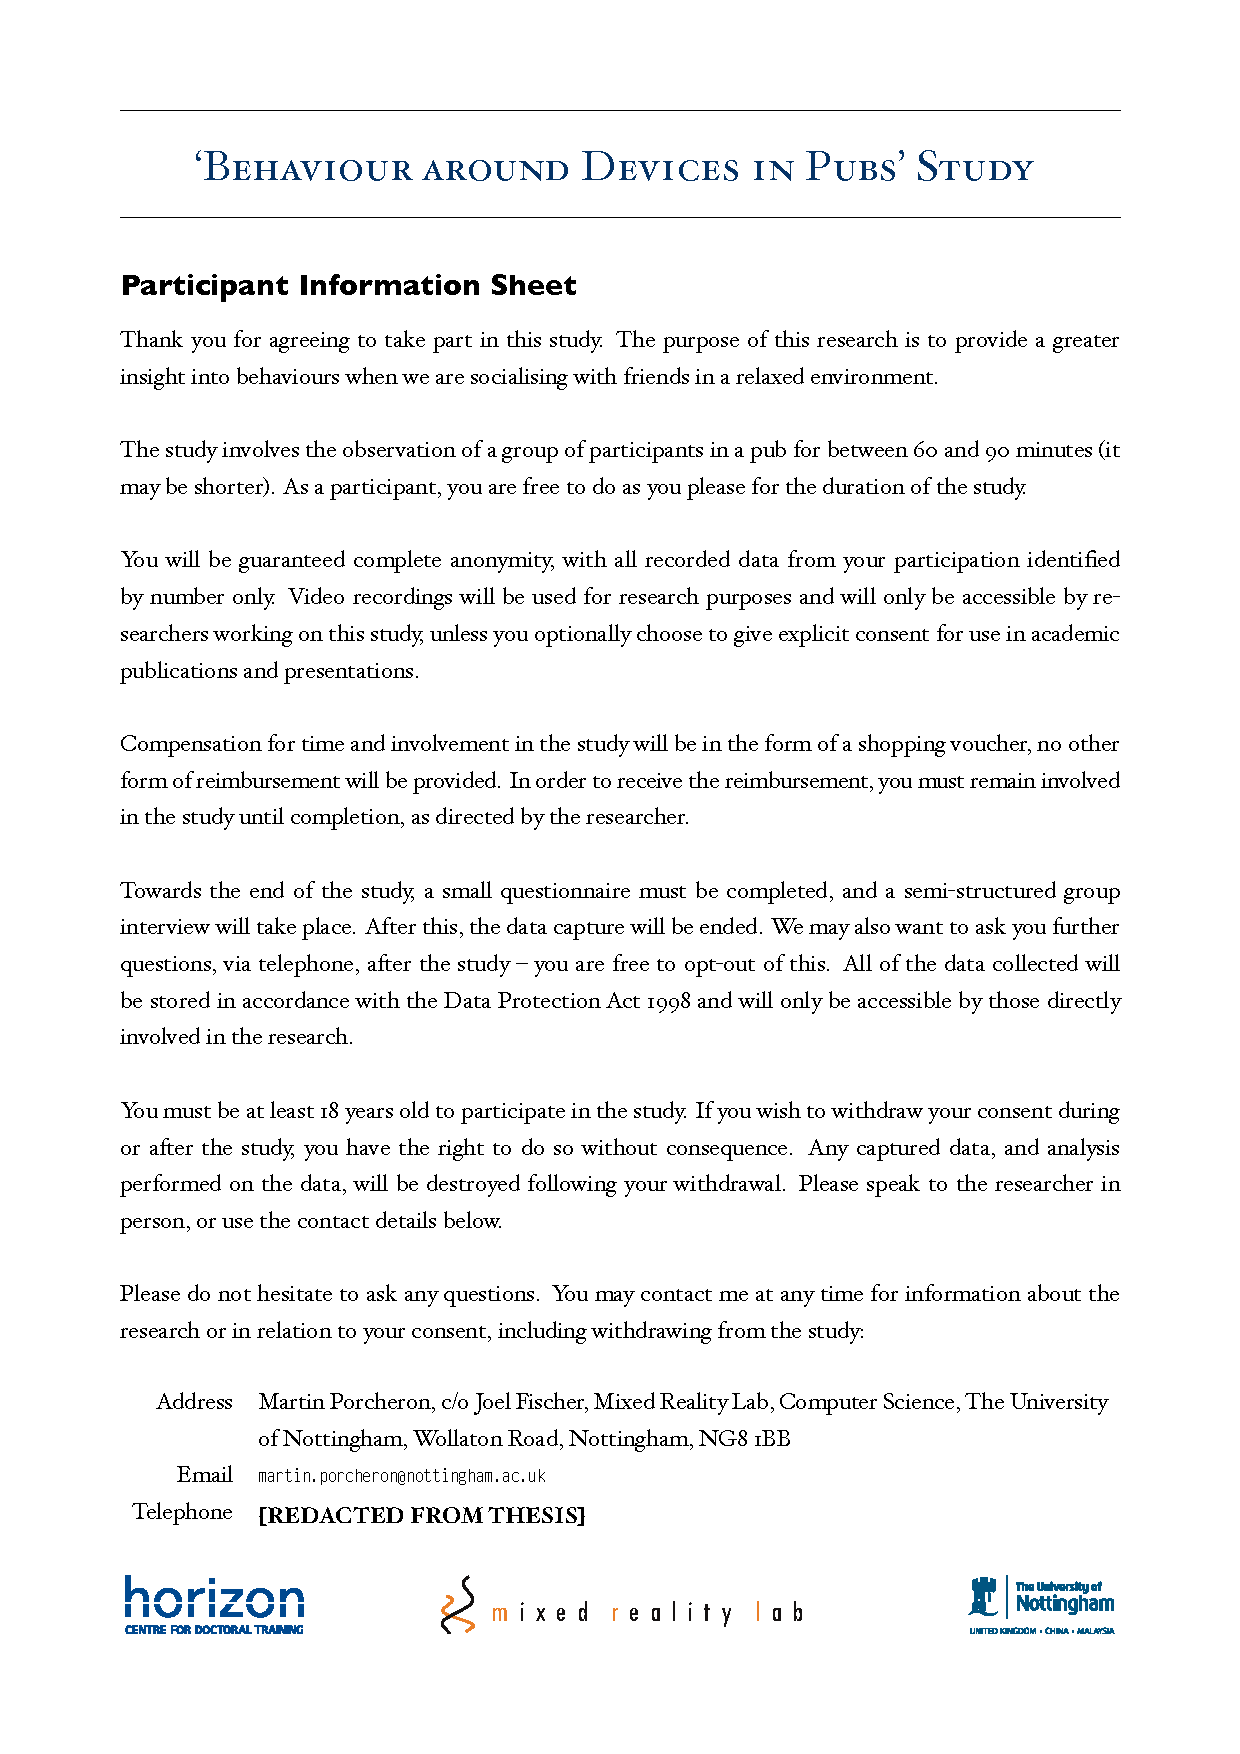
\includepdf[
    pages={1},
    scale=.6,
    frame=false,
    clip,
    trim=1.5cm 1.5cm 1.5cm 1.5cm,
    %offset=-1.05cm 0cm,
    pagecommand={\section{Information sheet and consent form}\label{app:studyinfo-pub infoconsent}}]
    {Graphics/A-StudyInfo-Pub/InfoConsent.pdf}
\includepdf[
    pages={2},
    scale=.6,
    frame=false,
    clip,
    trim=1.5cm 1.5cm 1.5cm 1.5cm,
    %offset=-1.05cm 0cm,
    pagecommand={\nopagebreak}]
    {Graphics/A-StudyInfo-Pub/InfoConsent.pdf}



% *********************************************************************************************************************



\section{Exit interview questions}\label{app:studyinfo-pub interview}

\begin{itemize}
    \item How do you feel about the presence of phones in social settings?
    \item Would you say the presence of devices has an impact on the conversation?
    \item Do you recall a time when you have felt ignored by someone using their phone?
    \item How feel about devices attempting to stop you using them at inopportune moments?
    \item Do you see any merits in devices attempting to restrict usage?
    \item Do you feel that people have a responsibility to the group dynamic?
    \item Would you categorise mobiles as a support tool or a distraction device
    \item Could you see mobile phones being used in conversation without detracting from it?
    \item Would you be willing to take part in further studies that required the installation of an app?
    \item Were you disturbed by presence of cameras or recording equipment?
    \item Did you feel you acted unnaturally due to nature of study?
    \item Did you remain aware of the presence of camera?
\end{itemize}



% *********************************************************************************************************************


% \includepdf[
%     pages={1},
%     scale=.6,
%     frame=false,
%     clip,
%     trim=1.5cm 1.5cm 1.5cm 1.5cm,
%     pagecommand={\section{Questionnaire}\label{app:studyinfo-pub questionnaire}}]
%     {Graphics/A-StudyInfo-Pub/Questionnaire.pdf}
% \includepdf[
%     pages={2},
%     scale=.6,
%     frame=false,
%     clip,
%     trim=1.5cm 1.5cm 1.5cm 1.5cm,
%     %offset=-1.05cm 0cm,
%     pagecommand={\nopagebreak}]
%     {Graphics/A-StudyInfo-Pub/Questionnaire.pdf}



% *********************************************************************************************************************



\section{Data session guidance}\label{app:studyinfo-pub datasession}



% *********************************************************************************************************************



\paragraph{Setting} \hfill \\
The recordings for this data session were made in a Nottingham-based pub, near to the university, during normal opening hours.
The majority of the recordings took place in the afternoon when the pub was relatively quiet.

A table that was in the corner of pub was chosen for the groups to sit at, and two GoPro cameras were positioned to capture all those present at the table.
One camera was positioned on a tripod and the other was positioned on a ledge within the pub.
An audio recorder was placed on the table to capture higher-quality audio.

Groups of 3 or 4 friends were recruited through email and word-of-mouth communication to participate in a study that involved “going to the pub”.
There were no prerequisites other than that all members of the group should be friends; groups were purposefully told minimal information before the study, other that what was required by the ethics committee.

Upon arrival at the pub, groups were greeted and invited to sort drinks out before taking their seats.
Consent forms were completed, and an opportunity for individuals to ask questions was provided.
The common question amongst groups was whether any tasks were required and this was answered accordingly.

The researcher sat at the table and engaged with the group where appropriate.



% *********************************************************************************************************************



\paragraph{Focus} \hfill \\
The focus of this research is to discover the interactional methods through which devices are topicalised, then sustained/co-oriented to, and then disengaged from, within social collocated interactions.



% *********************************************************************************************************************

%!TEX root = ../PhDThesis.tex



% *********************************************************************************************************************
\chapter{Transcript Notation}\label{app:notation}
% *********************************************************************************************************************



In general, the orthographic notation for fragments of transcribed data is based upon the system employed by \citet{Heath2010}.
However, a number of differences and simplifications have been made for brevity, clarity, and conciseness.
This notation itself was derived from the notation system originally described by \citet{Atkinson1984a}, devised by Gail Jefferson, and often used in Conversation Analysis-related literature.

Summarily, the notation used for transcribed data in this thesis adopts the following conventions:

\begin{itemize}
\item the volume of talk is denoted as \texttt{LOUD} or \texttt{\degree{quiet}\degree},
\item emphasis is denoted with \texttt{\underline{underlined text}},
\item shifts in intonation are given as arrows, i.e. \texttt{$\uparrow$} for a rising intonation and \texttt{$\downarrow$} for a falling intonation,
\item a single dash (\texttt{-}) when an utterance is cut off,
\item an equals (\texttt{=}) at the end of an utterance and at the start of a following utterance to denote contiguous talk (indentation is used to improve clarity and readability in these cases),
\item elongation of sounds and words are like \texttt{th::is}, where the \texttt{th} sound is two-tenths of a second in length,
\item pauses between words and utterances are given as \texttt{(.)}, where each individual period represents a tenth of a second; or as \texttt{(0.4)}, where this represents a pause of 0.4 seconds,
\item overlapping talk or action is denoted using opening square brackets (\texttt{[}) and closing square brackets (\texttt{]}) where possible or applicable (sometimes this closing bracket is omitted if two concurrent utterances end simultaneously at an end of a turn),
\item indentation is often used with overlapping talk or action to aid readability,
\item actions are given in \texttt{((double parentheses))},
\item utterances to an electronic device as a query (i.e. as input to the device) are given as \texttt{\textbf{bold text}},
\item digitally produced spoken words from an electronic device are preceded and succeeded with two forward slashes and typed in \texttt{\textit{// italics // }}, and
\item Names are typically denoted using the first three letters from the first name of the participant, e.g. \texttt{LIL} for \textit{Lily}; the researcher is identified as \texttt{RES}.
\end{itemize}



% *********************************************************************************************************************

%!TEX root = ../PhDThesis.tex



% *********************************************************************************************************************
\chapter{Fragments from the first study}\label{app:fragments-pub}
% *********************************************************************************************************************



\resubmission{This appendix is new, and includes the complete fragments from the pub talk chapter}
This appendix includes the full fragments presented over a number of excerpts in \autoref{ch:empirical pub}. There are three fragments:

\begin{itemize}
    \item \appref{app:fragments-pub schnauzers} is the transcript for the \textit{Miniature Schnauzers} fragment, which is composed of Data Excerpts \ref{frag:empirical pub findings newinfo-i}, \ref{frag:empirical pub findings newinfo-ii}, \ref{frag:empirical pub findings newinfo-iii}, and \ref{frag:empirical pub findings newinfo-iv};
    \item \appref{app:fragments-pub fontsize} is the transcript for the \textit{Font Size} fragment, which is composed of Data Excerpts \ref{frag:empirical pub findings joke-i}, \ref{frag:empirical pub findings joke-ii}, and \ref{frag:empirical pub findings joke-iii}; and
    \item \appref{app:fragments-pub shorthand} is the transcript for the \textit{Shorthand} fragment, which is composed of Data Excerpts \ref{frag:empirical pub findings contest-i}, \ref{frag:empirical pub findings contest-ii}, and \ref{frag:empirical pub findings contest-iii}.
\end{itemize}

% *********************************************************************************************************************

\section{Miniature Schnauzers}\label{app:fragments-pub schnauzers}
\begin{inlinefrag*} 
    \begin{transcript*}
        \by CAL {i like miniature schnauzers} \\
        \by DAY {°how big are schn-?°} \\
        \im 2   {Graphics/3-1-Empirical-Pub/FragmentSchnauzer-1.png}
        \by CAL {it's like (.) like (.) they're} \\
        \by     {\emph{so:} cute\vspace{2cm}} \\*
        \im 1   {Graphics/3-1-Empirical-Pub/FragmentSchnauzer-2.png}
        \by CAL {((briefly looks at her bag to} \\
        \by     {her left before looking back))} \\*
        \by DAY {i like big dogs\vspace{1.9cm}} \\*
        \im 2   {Graphics/3-1-Empirical-Pub/FragmentSchnauzer-3.png}
        \by CAL {i know, but google schnauzer,} \\
        \by     {right?} \\*
        \by DAY {((gets phone out from bag))} \\*
        \by CAL {((leans towards DAY)) } \\
        \by     {the puppies (.) schnauzer} \\
        \by     {puppies are gorgeous} \\
        \later  {\ldots} \\
        \by CAL {so it's miniature schnauzer} \\
        \by DAY {how do you?=} \\
        \im 1   {Graphics/3-1-Empirical-Pub/FragmentCollabSearch-2.png}
        \by CAL {~~~~~~~~~~~~=erm::} \\
        \by DAY {(sccchhhh) (tea) (ee) (ar)} \\
        \by CAL {oh schnauzer (.)} \\
        \by     {it's s-c-h-n-a-u-z- n-a-u-} \\
        \by     {(2.2) schnauzer} \\
        \by DAY {oh, sch\emph{nauz}er\vspace*{.4cm}} \\
        \im 1   {Graphics/3-1-Empirical-Pub/FragmentCollabSearch-4.png}
        \by CAL {schnauzer, go look at} \\
        \by     {schnauzer puppies right\intUp} \\
        \by     {((continues to look at phone))}\\
        \by DAY {°my internet is rubbish so} \\
        \by     {this may take some time°} \\
                \by DAY {((looks down and unlocks} \\
        \by     {phone)) \intDown oh tha\emph{t}: thing } \\
        \im 1   {Graphics/3-1-Empirical-Pub/FragmentSchnauzer-5.png} 
        \by CAL {((leans towards DAY and} \\
        \by     {shifts gaze towards her} \\
        \by     {screen)) yes look at them} \\
        \by     {oo:::\intUp} \\
        \by DAY {\quiet{schanuzer}\vspace*{1.6cm}}
    \end{transcript*}
\end{inlinefrag*}

% *********************************************************************************************************************



\section{Font Size}\label{app:fragments-pub fontsize}
\begin{inlinefrag*} 
    \begin{transcript*}
        \im 2   {Graphics/3-1-Empirical-Pub/FragmentEmail-2.png}
        \by JAY {beginning of september they} \\
        \by     {had their (.) all their} \\
        \by     {christmas stuff out (.) and I} \\
        \by     {was °like oh my god nobody} \\
        \by     {(\qquad \qquad \qquad )°} \\
        \im 3   {Graphics/3-1-Empirical-Pub/FragmentEmail-3.png}
        \by LAW {°jesus!°} \\*
        \by JAY {we just booked ours (1.0) we} \\
        \by     {do me and liam and james and} \\
        \by     {malcolm do (one every year and} \\
        \by     {we) just booked it} \\*
        \by MAL {du bois\intUp} \\*
%        \im 1   {Graphics/3-1-Empirical-Pub/FragmentEmail-4.png}
        \by LAW {=sorry (.) have you (.) um (.)} \\
        \by     {((jovially)) jonathan has sent} \\
        \by     {round an email (.) this is} \\
        \by     {great for your study isn't it?} \\
        \im 1   {Graphics/3-1-Empirical-Pub/FragmentEmail-4.png}
        \by RES {going to have to zoom in for} \\
        \by     {the camera (.) it's only set} \\
        \by     {to 720p!} \\
        \by JAY {mu:::::a::h} \\
        \by LAW {yeah (.) that's (.) that (.)} \\
        \by     {that's the email!-} \\
        \later  {\ldots}[4] \\
        \by MAL {is that him or is that your} \\
        \by     {phone fitting the line in?} \\
    \end{transcript*}
\end{inlinefrag*}

% *********************************************************************************************************************

% *********************************************************************************************************************



\section{Shorthand}\label{app:fragments-pub shorthand}
\begin{inlinefrag*} 
    \begin{transcript*}
        \im 1   {Graphics/3-1-Empirical-Pub/FragmentShorthand-1.png}
        \by LAW {isn't it mainly phonetic?} \\
        \by JAY {it's like:\vspace*{1.65cm}} \\
        \later  {3.2} \\
        \im 1   {Graphics/3-1-Empirical-Pub/FragmentShorthand-2.png}
        \by JAY {there's various versions so} \\
        \by     {the one she tried to teach me} \\
        \by     {first so i could start going} \\
        \by     {is missing out all the vowels} \\
        \by  LAW {((briefly looks at JAY while } \\
        \by      {picking up his phone, he then} \\
        \by      {(begins to use his phone once } \\
        \by      {he has it in his hands))} \\
        \by LAW {\intDown{}yeah} \\
        \im 1   {Graphics/3-1-Empirical-Pub/FragmentShorthand-4.png}
        \by JAY {and once you get good at that} \\
        \by     {you just write a lot quicker} \\
        \by     {(0.7) but then she had one} \\
        \by     {which was literally like (.)=} \\*
        \by LAW {\intDown{}yeah} \\
        \by JAY {=swiggles and just didn't look} \\
        \by     {like anything and i don't know} \\
        \by     {if that's phonetic or::::} \\
        \by MAL {(\qquad \qquad \qquad \qquad )} \\
        \im 1   {Graphics/3-1-Empirical-Pub/FragmentShorthand-5.png}
        \by LAW {hang on! ((typing on phone} \\
        \by     {with thumbs)) schuh::::::::ort} \\
        \by     {(.....) hand (..)} \\
        \by     {my mum's regular handwriting} \\
        \by RES {i know some people who miss} \\
        \by     {out vowels (.) like the e\vspace*{.7cm}} \\
        \im 1   {Graphics/3-1-Empirical-Pub/FragmentShorthand-6.png}
        \by JAY {that's how i do it (.) missing} \\
        \by     {out vowels is very very good} \\
        \by     {but there's a squiggly one i} \\
        \by     {don't understand} \\
        \by MAL {this is why i didn't do} \\
        \by     {ethnography (1.8) just get the} \\
        \by     {participants to fill} \\
        \by     {everything out} \\
        \by LAW {i didn't do ethnography either} \\
        \by     {either!} \\
        \by MAL {yeah\intUp{} you do it- i'm not- i'm} \\
        \by     {not doing=} \\
        \im 1   {Graphics/3-1-Empirical-Pub/FragmentShorthand-7.png}
        \by LAW {=oo\intUp{} that's got (2.0) that's} \\
        \by     {cinnamon in it or something} \\
        \by     {something (..) smells amazing\vspace*{1cm}}
    \end{transcript*}
\end{inlinefrag*}

% *********************************************************************************************************************

%!TEX root = ../PhDThesis.tex



% *********************************************************************************************************************
\chapter{Additional information about the second study}\label{app:studyinfo-cafe}
% *********************************************************************************************************************



This appendix includes additional material to the second study of \acf{VUI} use in a caf\'e (see \autoref{ch:empirical cafe}):

\begin{itemize}
    \item \appref{app:studyinfo-cafe infoconsent} provides the information sheet and consent form given to participants prior to the study,
    \item \appref{app:studyinfo-cafe interview} provides the post-observation interview questions, and
    \item \appref{app:studyinfo-cafe questionnaire} provides the post-observation questionnaire.
\end{itemize}

Additional material related to the study is available on the accompanying CD and online repository:

\begin{itemize}
    \item The descriptive results from the questionnaire are provided in \texttt{studytwo/questionnaire.pdf}.
\end{itemize}



% *********************************************************************************************************************




\includepdf[
    pages={1},
    scale=.6,
    frame=false,
    clip,
    trim=1.5cm 1.5cm 1.5cm 1.5cm,
    %offset=-1.05cm 0cm,
    pagecommand={\section{Information sheet and consent form}\label{app:studyinfo-cafe infoconsent}}]
    {Graphics/C-StudyInfo-Cafe/InfoConsent.pdf}
 
\includepdf[
    pages={2},
    scale=.6,
    frame=false,
    clip,
    trim=1.5cm 1.5cm 1.5cm 1.5cm,
    %offset=-1.05cm 0cm,
    pagecommand={\nopagebreak}]
    {Graphics/C-StudyInfo-Cafe/InfoConsent.pdf}



% *********************************************************************************************************************



\section{Exit interview questions}\label{app:studyinfo-cafe interview}

\begin{itemize}
    \item How do you feel about the presence of phones in social settings?
    \item Would you say the presence of devices has an impact on the conversation?
    \item Do you recall a time when you have felt ignored by someone using their phone?
    \item How feel about devices attempting to stop you using them at inopportune moments?
    \item Do you see any merits in devices attempting to restrict usage?
    \item Do you feel that people have a responsibility to the group dynamic?
    \item Would you categorise mobiles as a support tool or a distraction device?
    \item Could you see mobile phones being used in conversation without detracting from it?
    \item Would you be willing to take part in further studies that required the installation of an app?
    \item Were you disturbed by presence of cameras or recording equipment?
    \item Did you feel you acted unnaturally due to nature of study?
    \item Did you remain aware of the presence of cameras?
\end{itemize}



% *********************************************************************************************************************



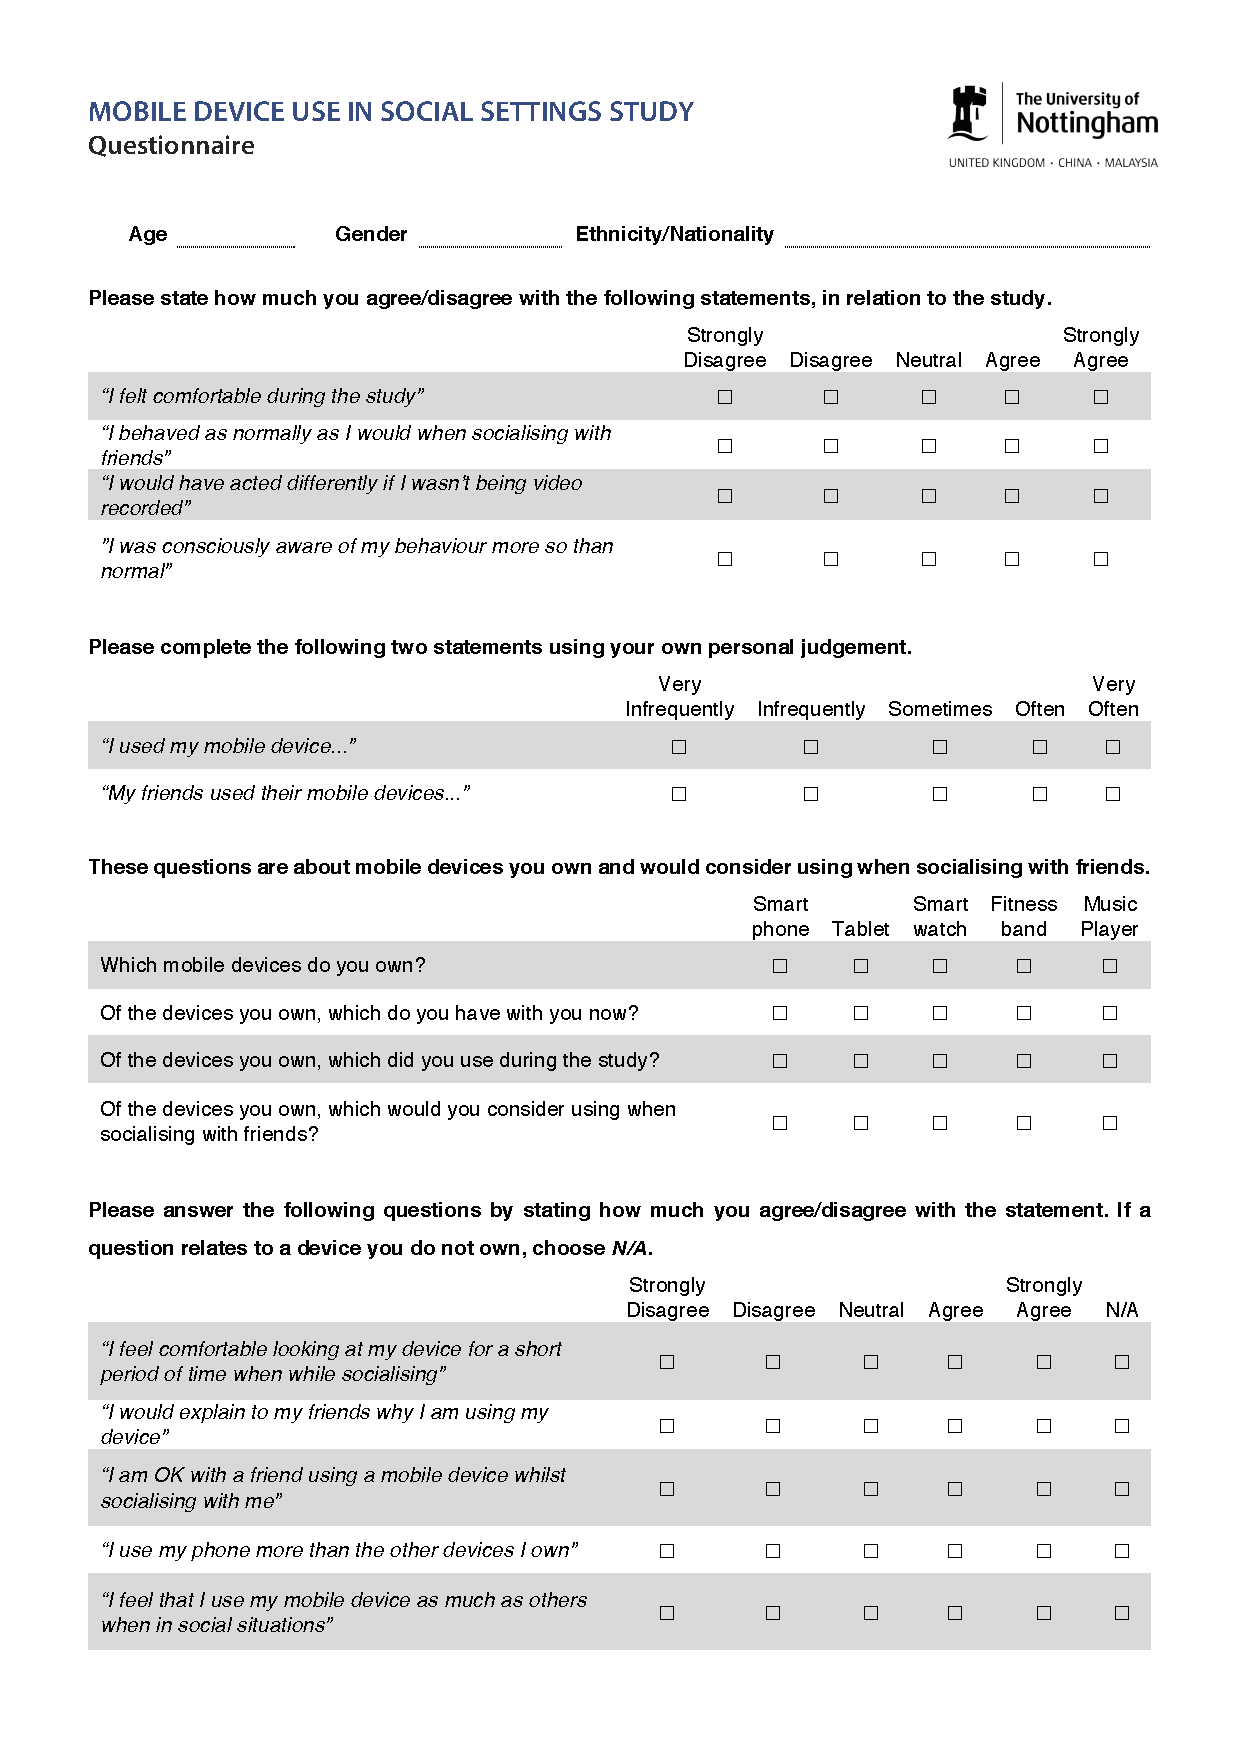
\includepdf[
    pages={1},
    scale=.6,
    frame=false,
    clip,
    trim=1.5cm 1.5cm 1.5cm 1.5cm,
    %offset=-1.05cm 0cm,
    pagecommand={\section{Questionnaire}\label{app:studyinfo-cafe questionnaire}}]
    {Graphics/C-StudyInfo-Cafe/Questionnaire.pdf}



% *********************************************************************************************************************

%!TEX root = ../PhDThesis.tex



% *********************************************************************************************************************
\chapter{Fragments from the second study}\label{app:fragments-cafe}
% *********************************************************************************************************************



\resubmission{This appendix is new, and includes the complete fragments from the cafe talk chapter}
This appendix includes the full fragments presented over a number of excerpts in \autoref{ch:empirical cafe}. There are three fragments:

\begin{itemize}
    \item \appref{app:fragments-cafe sunset} is the transcript for the \textit{When Does the Sun Go Down?} fragment, which is composed of Data Excerpts \ref{frag:empirical cafe findings newinfo-i}, \ref{frag:empirical cafe findings newinfo-ii}, and \ref{frag:empirical cafe findings newinfo-iii};
    \item \appref{app:fragments-cafe animals} is the transcript for the \textit{Do Animals Have Accents?} fragment, which is composed of Data Excerpts \ref{frag:empirical cafe findings answering-i}, \ref{frag:empirical cafe findings answering-ii}, \ref{frag:empirical cafe findings answering-iii}, and \ref{frag:empirical cafe findings answering-iv}; and
    \item \appref{app:fragments-cafe mama} is the transcript for the \textit{Hey Siri! \ldots Call My Mother} fragment, which is composed of Data Excerpts \ref{frag:empirical cafe findings capability-i} and \ref{frag:empirical cafe findings capability-ii}.
\end{itemize}

% *********************************************************************************************************************

\section{When Does the Sun Go Down?}\label{app:fragments-cafe sunset}
\begin{inlinefrag} 
    \begin{transcript}
        \by HAR {i’ll be fine in like three minutes ((holds hands in front of} \\
        \by     {eyes))} \\
        \by RES {keeps coming back as well like} \\
        \by SAL {as soon as you cha\emph{nge} it comes back} \\
        \by JUL {yeah yeaha} \\
        \later  {0.3} \\
        \by RES {there’s actually just someone out there with a light!} \\
        \by ALL {((laugh))} \\
        \later {\ldots}[7] \\
        \by JUL {[ ((removes cover from device but leaves open)) ]} \\
        \by SAL {((laughs))} \\
        \by JUL {((presses button on device))} \\
        \by HAR {there we go!} \\
        \by JUL {\textbf{what’s the time of sunset?}} \\
        \later  {1.3} \\
        \by ALL {((gaze at the tablet))} \\
        \later  {3.0} \\
        \by JUL {ok! \textit{// ((device displays clock)) //}} \\
        \by ART {((leans in to look))} \\
        \by SAL {that’s [ a~~~~~~] fucking analogue clock it pisses me off!} \\
        \by HAR {~~~~~~~[ today? ]} \\
        \by HAR {ilunno (0.6) 24 hour=} \\
        \by JUL {<no no no!> it misunderstood actually (0.8) understood what’s} \\
        \by     {the [ time ]} \\
        \by HAR {~[ time ] now} \\
        \by JUL {so-} \\
        \by ART {soaoah yeah\intUp} \\
        \by JUL {shall i ask (1.6) um:=} \\
        \by HAR {~~~~~~~~~~~~~~~~~~~~~=what time will the [ sun set? ]} \\
        \by JUL {~~~~~~~~~~~~~~~~~~~~~~~~~~~~~~~~~~~~~~~~~[ ((holds button)) ]} \\
        \by JUL {\textit{// ((audible chime)) //}} \\
        \later  {4.0} \\
        \by JUL {\textit{ // ((on screen text: go ahead i’m listening\ldots)) //}} \\
        \later  {0.3} \\
        \by JUL {\textbf{when does the sun go down?}} \\
        \later  {2.9} \\
        \by JUL {sunset will be at [ seventeen thirty two ]} \\
        \by ART {~~~~~~~~~~~~~~~~~~[ ther:::e you go~~~~~~]} \\
    \end{transcript}
    \begin{center}
            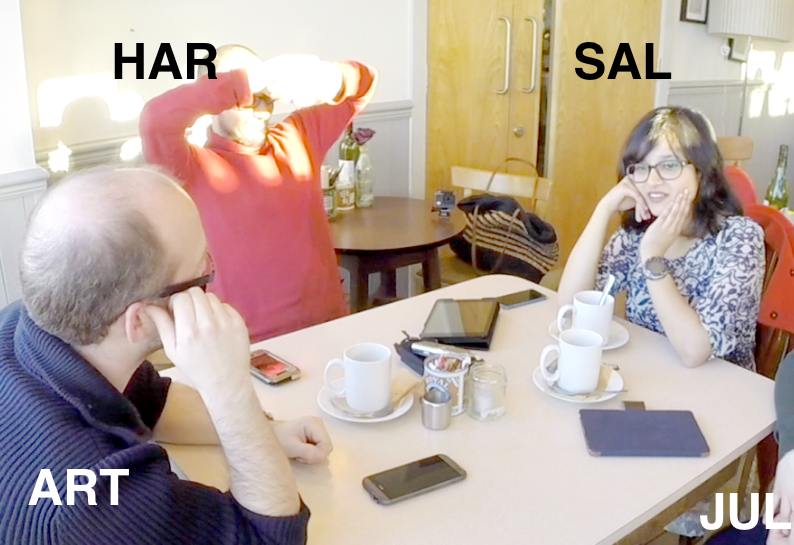
\includegraphics[width=.5\linewidth]{Graphics/3-2-Empirical-Cafe/FragmentSunset-1}\\
            (line 1)\\[1cm]
            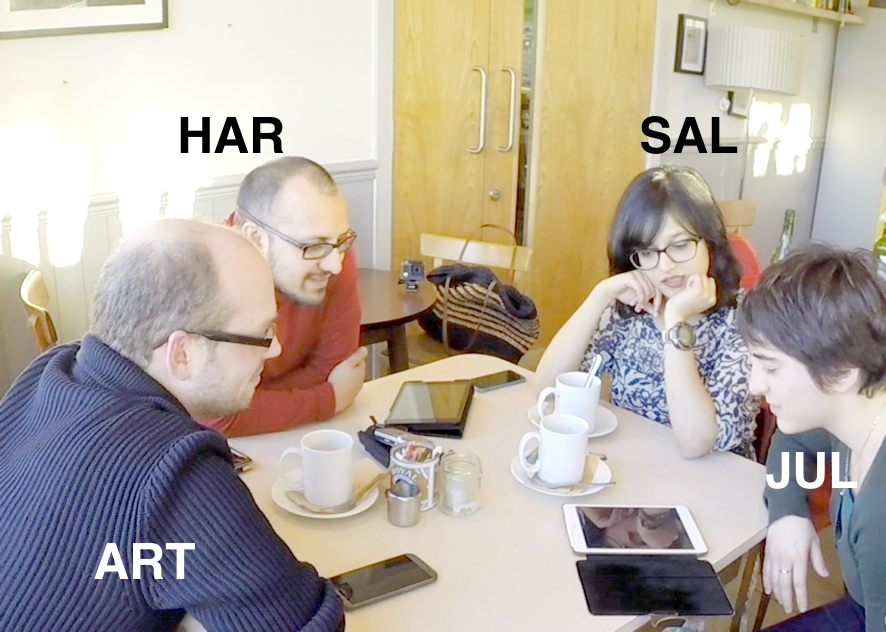
\includegraphics[width=.5\linewidth]{Graphics/3-2-Empirical-Cafe/FragmentSunset-2}\\
            (line 25)
    \end{center}
\end{inlinefrag}

% *********************************************************************************************************************



\section{Do Animals Have Accents?}\label{app:fragments-cafe animals}
\begin{inlinefrag} 
    \begin{transcript}
        \by KAR {do cats acth- (0.5) can you work out whether it's french because} \\
        \by     {because its talking in a- doing a french cat impression} \\
        %\im    1 {Graphics/3-2-Empirical-Cafe/FragmentAnimals-1.png}
        \by LIL {i::::: think some animals you can} \\
        \later {1.9} \\
        \by LIL {((picks up phone from table))} \\
        \later {\ldots}[34] \\
        \by LIL {er:::m: ((holding phone in front of her at chest level))} \\
        \later  {3.7} \\
        %\im    3 {Graphics/3-2-Empirical-Cafe/FragmentAnimals-2.png}
        \by LIL {((moves phone up to face)) \textbf{do animals have acce\emph{nts}?}} \\
        \later  {2.1} \\
        \by GAR {((shifts gaze to LIL))} \\
        \by     {yes they do actually! i think i've read something} \\
        \by LIL {i think i have [ too\intDown{}~~]} \\
        \by GAR {~~~~~~~~~~~~~~~[ yeas!~] [ (0.6) \emph{cows}! i- i~~~~~~~~~~~~~~~]} \\
        \by     {~~~~~~~~~~~~~~~~~~~~~~~~~read about cows that they have} \\
        \by     {~~~~~~~~~~~~~~~~~~~~~~~~~different accents around the world} \\
        \by KAR {~~~~~~~~~~~~~~~~~~~~~~~~~[ you missed mine- my racist joke ]} \\
        \by LIL {\textbf{DO: \emph{ANIM}ALS HA\emph{V}E \emph{ACCEN}TS!}} \\
        \later  {2.4} \\
        \by LIL {°rubbish°=} \\
        \by KAR {~~~~~~~~~~~=parrots presumably do=} \\
        \by LIL {~~~~~~~~~~~~~~~~~~~~~~~~~~~~~~~~~~=can you ask it?} \\
        \by     {((holds phone out in front of KAR's face))} \\
        %\im    1 {Graphics/3-2-Empirical-Cafe/FragmentAnimals-3.png}
        \by RES {((retrieves phone out of pocket))} \\
        \by KAR {\textbf{DO: ANI\emph{MALS} HAVE ACC::\emph{ENT}S!}} \\
        \later  {0.9} \\
        \by LIL {no:!} \\
        \by RES {\textit{//~sorry i'm-~//}} \\
        \by RES {((RES touches screen to stop utterance))} \\
        \by RES {\textbf{do animals have accents?}} \\
        \by LIL {\textbf{d\emph{o:} \emph{anim}als ha\emph{v}e a\emph{ccents}?}} \\
        \by RES {\textit{//~ok i've found this on the web~//} (sigh)} \\
        \by GAR {do [ they?~~]} \\
        \by LIL {~~~[ ah (.) ] it's working now!} \\
    \end{transcript}

    \begin{center}
            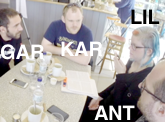
\includegraphics[width=.7\linewidth]{Graphics/3-2-Empirical-Cafe/FragmentAnimals-2}\\
            (line 44)\\[1cm]
            
\includegraphics[width=.7\linewidth]{Graphics/3-2-Empirical-Cafe/FragmentAnimals-3}\\
            (line 56)
    \end{center}
\end{inlinefrag}

% *********************************************************************************************************************

% *********************************************************************************************************************



\section{Hey Siri! \ldots Call My Mother}\label{app:fragments-cafe mama}
\begin{inlinefrag*} 
    \begin{transcript*}
        \by GAR {i'm curious if I say in} \\
        \by     {romanian (.) to call my mother} \\
        \later {0.7} \\
        \by GAR {it will actually find the } \\
        \by     {contact for my mother is (.)} \\
        \by     {mama in romanian (.) if I say} \\
        \by     {call my mum will it actually} \\
        \by     {call my mother which is in a} \\
        \by     {contact as mama (0.7) will it} \\
        \by     {make the connection between} \\
        \by     {mama and mum} \\
        \by RES {cos you can also tell people} \\
        \by     {who they (.) like you can say} \\
        \by     {like\vspace*{1cm}} \\
        \im 1   {Graphics/3-2-Empirical-Cafe/FragmentMamma-1.png}
        \by GAR {\textbf{hey siri=}} \\
        \by RES {~~~~~~~~~=my mother is this} \\
        \by     {~~~~~~~~~~person (0.8)} \\
        \by GAR {((glances down at screen))} \\
        \by     {((moves device in front of} \\
        \by     {mouth)) \textbf{hey siri}} \\
        \by GAR {((moves device to chest} \\
        \by     {height between the two))} \\
        \later  {1.0} \\
        \by RES {i'd press the button} \\
        \later  {1.2} \\
        \by GAR {((moves device in front of} \\
        \by     {mouth)) \textbf{hey siri}} \\
        \by GAR {((moves device to chest} \\
        \by     {height between the two))} \\
        \later  {2.4} \\
        \by GAR {((moves device in front of} \\
        \by     {mouth)) \textbf{call my \emph{m}other}} \\
        \im 1   {Graphics/3-2-Empirical-Cafe/FragmentMamma-2.png}
        \by     {((GAR and RES look at screen))}  \\
        \later  {5.9} \\
        \by     {\textit{// what is your mother's}} \\
        \by     {\textit{~~~name? //}} \\
        \by RES {((points towards screen)) yeah} \\
        \by     {but then} \\
        \later  {0.9} \\
        \by GAR {\textbf{my mother is mama}} \\
        \by GAR {\textit{// i can’t find anyone called}} \\
        \by     {\textit{~~~mamma //}} \\
    \end{transcript*}
\end{inlinefrag*}

% *********************************************************************************************************************

%!TEX root = ../PhDThesis.tex



% *********************************************************************************************************************
\chapter{Additional information about the third study}\label{app:studyinfo-home}
% *********************************************************************************************************************



This appendix includes additional material to the third study of \acf{VUI} use in a home (see \autoref{ch:empirical home}):

\begin{itemize}
    \item \appref{app:studyinfo-home infoconsent} provides the information sheet and consent form given to participants prior to the study, and
    \item \appref{app:studyinfo-home helpguide} provides the Amazon Echo Help Guide produced for the study, and left with participant households.
\end{itemize}



% *********************************************************************************************************************




\includepdf[
    pages={1},
    scale=.6,
    frame=false,
    clip,
    trim=1.5cm 1.5cm 1.5cm 1.5cm,
    pagecommand={\section{Information sheet and consent form}\label{app:studyinfo-home infoconsent}}]
    {Graphics/D-StudyInfo-Home/InfoConsent.pdf}

\includepdf[
    pages={2},
    scale=.6,
    frame=false,
    clip,
    trim=1.5cm 1.5cm 1.5cm 1.5cm,
    pagecommand={\nopagebreak}]
    {Graphics/D-StudyInfo-Home/InfoConsent.pdf}



% *********************************************************************************************************************



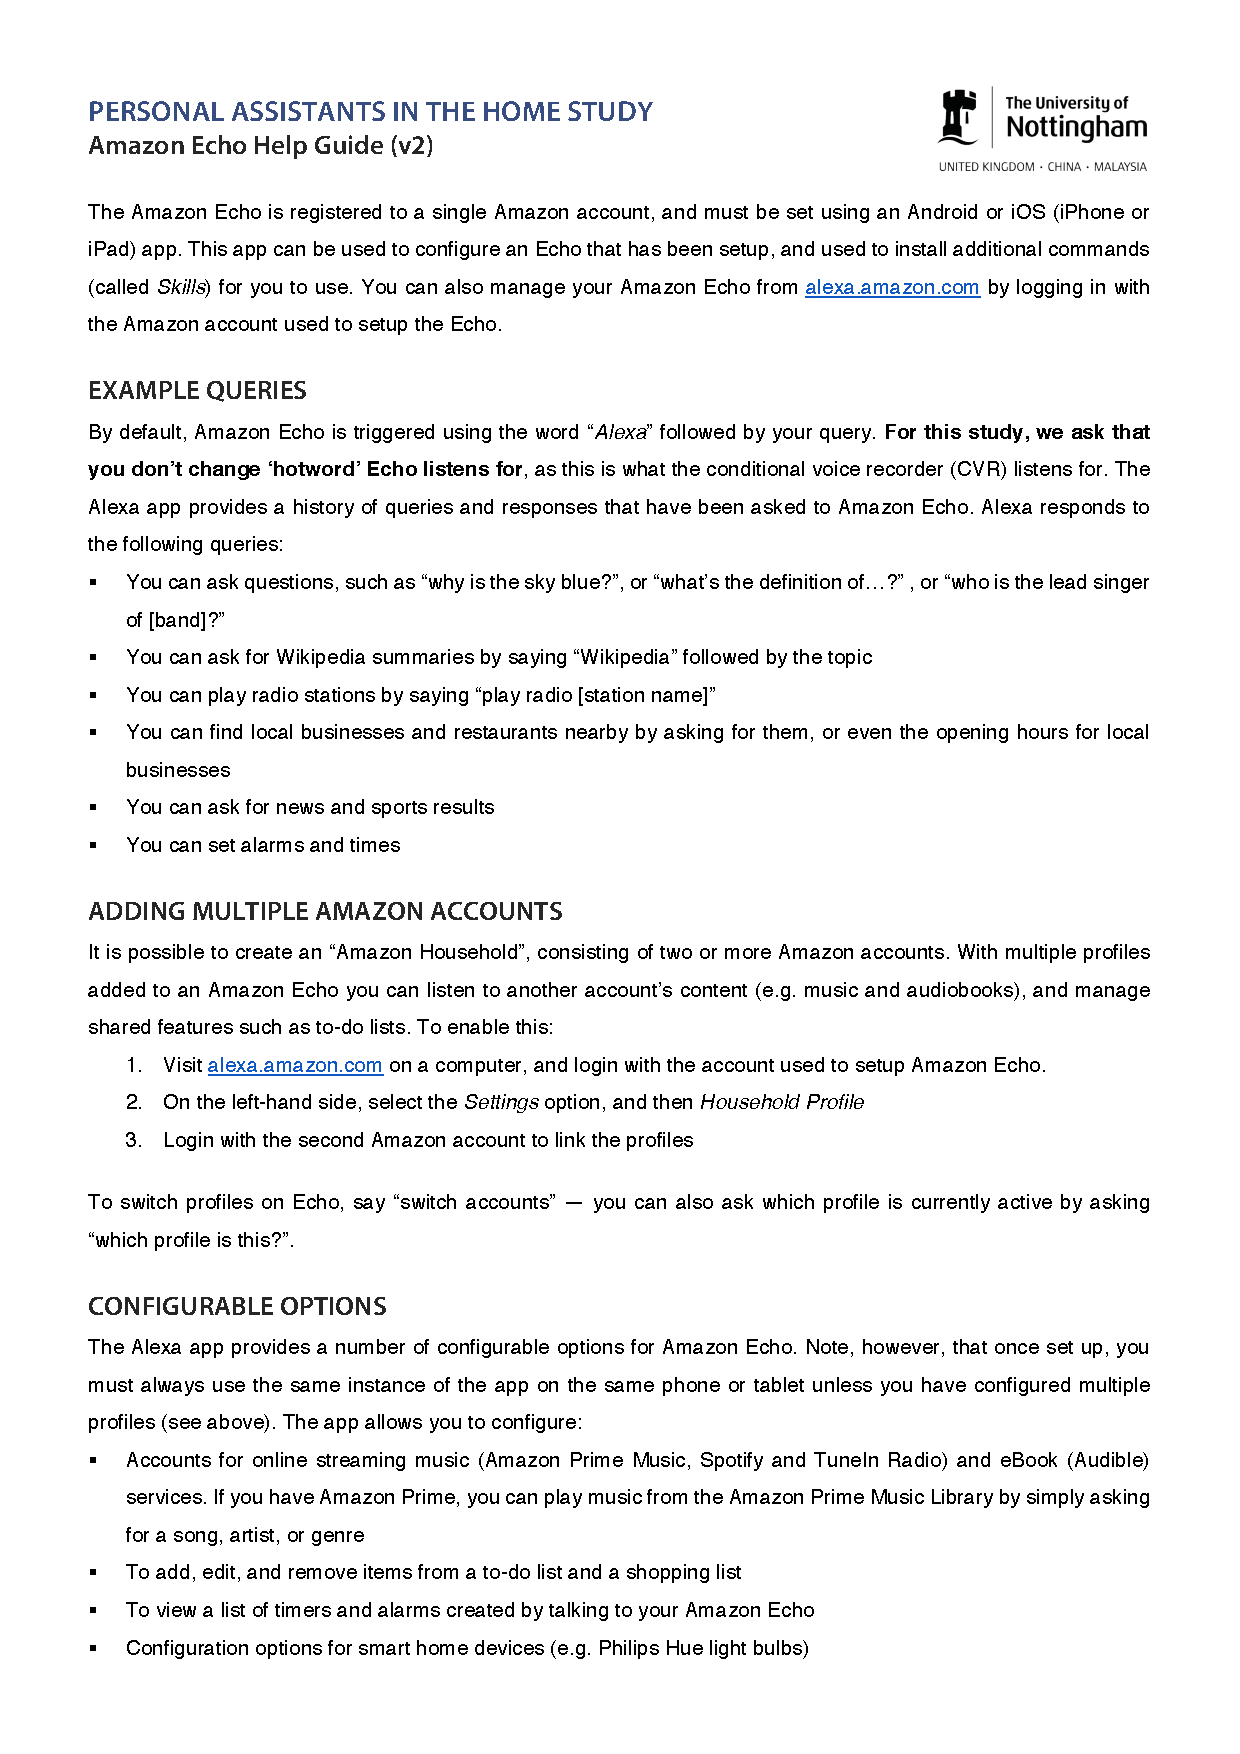
\includepdf[
    pages={1},
    scale=.6,
    frame=false,
    clip,
    trim=1.5cm 1.5cm 1.5cm 1.5cm,
    pagecommand={\section{Amazon Echo help guide}\label{app:studyinfo-home helpguide}}]
    {Graphics/D-StudyInfo-Home/AmazonEchoHelpGuide.pdf}
\includepdf[
    pages={2},
    scale=.6,
    frame=false,
    clip,
    trim=1.5cm 1.5cm 1.5cm 1.5cm,
    pagecommand={\nopagebreak}]
    {Graphics/D-StudyInfo-Home/AmazonEchoHelpGuide.pdf}



% *********************************************************************************************************************


% \section{Exit Interview Questions}\label{app:studyinfo-home interview}
% Exit Interviews with participants were performed roughly one-week after data capture ended, and was with the primary occupants of the household.
% The interview was split into two sections: (1) general questions, (2) reflection on selected queries.



% *********************************************************************************************************************


% \subsection*{General Questions}
% The following questions were asked to all participants in the study through a semistructured interview unless answered in a previous question.

% \begin{itemize}
%   \item What were your general impressions of using Echo in your home?
%   \begin{itemize}
%   \item Did you use it much?
%   \item Did you feel it affected your privacy?
%   \end{itemize}

%   \item What sort of queries did you ask of Echo?
%   \begin{itemize}
%   \item Who used it?
%   \item What did you use it for?
%   \item What did you ask?
%   \end{itemize}

%   \item How did you discover what questions you could ask?
%   \item Did you find the Echo was particularly good at recognising what you asked it to do?
%   \item When did you think the Echo was struggling?
%   \item Did Echo respond accordingly to what you asked it to do?
%   \item If you could ask Echo to do anything, what would it be? Were they times you wanted it to do something you couldn’t?
%   \item Were there times when Echo did stuff unexpectedly?

%   \item When Echo failed to respond to a query, how did find Echo’s response?
%   \item Did you understand what went wrong? Did you try and resolve the problem?

%   \item Did guests, friends, or other family members talk to Echo? Were you happy for this to happen?
%   \item Did they understand how to talk to it or did you provide explanations?
%   \item What sort of queries did they ask?
%   \item What was your experience of multiple people using Echo? Can you give an example?
% \end{itemize}

% \subsection*{Reflection on Selected Queries}
% A number of episodes were selected which involved potentially interesting findings, and each one was played to the participants as a probe to gauge further reflection.

% \begin{itemize}
%   \item Could you, in your own words, describe the interaction? What did you think about what happened?
%   \item What would you say motivated the query?
%   \item What did you think about Echo’s response?
%   \item How do you think Echo should have responded?
% \end{itemize}

% If query was worded by other than the interviewee(s), the following questions were asked:

% \begin{itemize}
%   \item How did you feel about the person asking the query?
%   \item What was your perception of Echo’s response?
% \end{itemize}

% If follow-up query was performed by other than the initial query performer, the following questions were asked:

% \begin{itemize}
%   \item What did you think about the follow-up query?
%   \item Why was the query repeated/refined? (choose appropriate)
%   \item How did you negotiate another person asking the query? (i.e. did it just happen or was it to explain or show people how it worked?)
% \end{itemize}



% *********************************************************************************************************************

%!TEX root = ../PhDThesis.tex



% *********************************************************************************************************************
\chapter{Fragments from the third study}\label{app:fragments-hoem}
% *********************************************************************************************************************



\resubmission{This appendix is new, and includes the complete fragments from the home talk chapter}
This appendix includes the full fragments presented over a number of excerpts in \autoref{ch:empirical home}. There are three fragments:

\begin{itemize}
    \item \appref{app:fragments-home greece} is the transcript for the \textit{Where is Greece?} fragment, which is composed of Data Excerpts \ref{frag:empirical home findings capability-i}, \ref{frag:empirical home findings capability-ii}, and \ref{frag:empirical home findings capability-iii};
    \item \appref{app:fragments-home nye-music} is the transcript for the \textit{New Year's Music} fragment, which is composed of Data Excerpts \ref{frag:empirical home findings music-i}, \ref{frag:empirical home findings music-ii}, and \ref{frag:empirical home findings music-iii}; and
    \item \appref{app:fragments-home beat-the-intro} is the transcript for the \textit{Beat the Intro} fragment, which is composed of Data Excerpts \ref{frag:empirical home findings game-i}, \ref{frag:empirical home findings game-ii}, and \ref{frag:empirical home findings game-iii}.
\end{itemize}

% *********************************************************************************************************************



\section{Where is Greece?}\label{app:fragments-home greece}
\begin{inlinefrag}
    \begin{transcript}
        \by LEA {\textbf{alexa (.) where is greece}} \\
        \later   {2.0} \\
        \by ALE {\textit{// greece is a un-recognised country in the northern hemisphere}} \\
        \by     {\textit{(.) it shares a border with turkey, albania, bulgaria}} \\
        \by     {\textit{and macedonia= //}} \\
        \by ISA {~~~~~~~~~~~~~=[ that’s it ]} \\
        \by LEA {~~~~~~~~~~~~~=[ that’s it ]} \\
        \later  {1.1} \\
        \by JOH {\textbf{alexa where is amfissa}} \\
        \later  {2.0} \\
        \by ALE {\textit{// amfissa is a city in phocidos (..) greece (.) it is 82 miles}} \\
        \by     {\textit{133 kilometres west of athens and 26 miles 42 kilometres south}} \\
        \by     {\textit{of lamia //}} \\
        \later  {0.5} \\
        \by JOH {\textbf{alexa where is (0.3) delph-ee}} \\
        \later  {7.0} \\
        \by ALE {\textit{// delph-i is a village in carroll county indiana (.) indiana (.)}} \\
        \by     {\textit{it is 62 miles 99 kilometres north of Indianapolis and 87 miles}} \\
        \by     {\textit{140 kilometres= //}} \\
        \by NIK {~~~~~~~~~~~~~~~\textbf{=alexa stop}} \\
    \end{transcript}
\end{inlinefrag}

% *********************************************************************************************************************

\section{New Year's Music}\label{app:fragments-home nye-music}
\begin{inlinefrag}
    \begin{transcript}
        \by NIK {\textbf{alexa}} \\
        \later  {2.6} \\
        \by ISA {\textbf{play some new year’s music}} \\
        \later  {1.8} \\
        \by ALE {\textit{// here’s a station for jazz music (.) instrumental jazz //}} \\
        \by     {\textit{((begins playing jazz music))}} \\
        \by ISA {\textbf{alexa this is not what we wanted}} \\
        \by     {[ ((laughs))~~~~~~~~~~~~~]} \\
        \by NIK {[ (1.2) \textbf{alexa} (1.1) \textbf{shut} ] \textbf{up!}} \\
        \by ISA {hey::\intUp (.) \textbf{alexa nikos apologises for being so rude}} \\
        \later  {0.3} \\
        \by ALE {hi there} \\
        \later  {1.0} \\
        \by     {[ \textit{((resumes playing jazz music)) }]} \\
        \by NIK {[ (2.4) \textbf{alexa stop} ~~~~~~~~~~~~~~] \textbf{stop!}} \\
    \end{transcript}
\end{inlinefrag}

% *********************************************************************************************************************

\section{Beat the Intro}\label{app:fragments-home beat-the-intro}
\begin{inlinefrag}
    \begin{transcript}
        \by SUS {i'd like to play beat the intro in a minute} \\
        \by LIA {[ oh no:: ]} \\
        \by SUS {[ \textbf{alexa}~~~][ (1.1)~~] \textbf{beat the in}[\textbf{tro}} \\
        \by CAR {~~~~~~~~~~~[ \quiet{yeah} ] } \\
        \by LIA {~~~~~~~~~~~~~~~~~~~~~~~~~~~~~~~~~[°no:::...°} \\
        \later {0.6} \\
        \by CAR {it's mother's day?} \\
        \later {0.4} \\
        \by SUS {it's (~~~~) yep (.) listen (.) you need to keep on eating your} \\
        \by     {orange stuff (.) liam} \\
        \later {0.7} \\
        \by CAR {and your green stuff} \\
        \by SUS {\textbf{alexa} (1.3) \textbf{alexa} (0.5)=} \\
        \by CAR { ~~~~~~~~~~~~~~~~~~~~~~=°and your brown stuff° } \\
        \by SUS {\textbf{play beat the intro}} \\
        \by EMM {°and the yellow stuff?°} \\
        \by LIA {°and the meat stuff°} \\
        \later  {0.9} \\
        \by ALE {\textit{// resuming the music //}} \\
        \by EMM {((laughs))} \\
        \by ALE {\textit{((music plays))}} \\
        \by SUS {oh no::!} \\
        \by EMM {((laughs))} \\
        \by CAR {\textbf{alexa stop:}} \\
        \by ALE {\textit{((stops playback))}} \\
        \by LIA {no::::::::::::} \\
        \by CAR {\textbf{ale}[\textbf{xa} (1.0)~~~~] \textbf{bea:t: the (.) in\underline{t}ro}} \\
        \by SUS {~~~[ ((laughs)) ]} \\
        \by SUS {it does it for you} \\
        \later {5.0} \\
        \by EMM {nope (.) she didn like tha:::::t} \\
        \by EMM {\textbf{alexsa} [ (1.0)~~~~~~~~~~~~~~~~~~~~~~~~] \textbf{play beat the \underline{in}tro::}} \\
        \by CAR {~~~~~~~[ is it called beat the intro? ]} \\
        \later {2.1} \\
        \by ALE {\textit{// you want to hear a station for b b intro [ (0.5) ] right? //}} \\
        \by EMM {~~~~~~~~~~~~~~~~~~~~~~~~~~~~~~~~~~~~~~~~~~~~[ \textbf{°no:°} ] } \\
        \later {1.1} \\
        \by EMM {\textbf{no:} (.) \textbf{i don't alex:a} (0.5) \textbf{no!}} \\
        \later {1.3} \\
        \by ALE {\textit{// alrig\intUp{}ht //}} \\
        \later {0.7} \\
        \by CAR {we played it the other ni:ght! the game we played} \\
        \by     {the [ other night ((laughs)) ]} \\
        \by SUS {~~~~[ yeaherr:: \textbf{alexa}~~~~~~~~] \textbf{skills} (.) \textbf{beat the intro}} \\
        \later {4.5} \\
        \by SUS {°uh::\intDown:° } \\
        \by EMM {she didn like tha:\intDown:t} \\
        \by SUS {\textbf{alechSA::::::}} \\
    \end{transcript}
\end{inlinefrag}

% *********************************************************************************************************************

% \section{Set us a Family Quiz}\label{app:fragments-home family-quiz}
% \begin{inlinefrag}
%     \begin{transcript}
%         \by EMM {can you ask for a normal quiz?} \\
%         \by SUS {\textbf{alexa} (0.7) \textbf{set us a family quiz}} \\
%         \later  {2.5} \\
%         \by ALE {\textit{// sorry (.) i can't find the answer to the question i heard //}} \\
%         \later  {0.4} \\
%         \by EMM {\textbf{ALech-sa:} (1.0) \textbf{\emph{set}:} (0.5) \textbf{a family quiz}} \\
%         \later  {2.3} \\
%         \by ALE {\textit{// sorry (.) i don't have the answer to that question //}} \\
%         \by SUS {°well°} \\
%         \by LIA {\textbf{alexa} (0.9) [ \textbf{\intUp{}PLease set} (0.4) \textbf{a family quiz} ]} \\
%         \by EMM {~~~~~~~~~~~~[ ((laughs))~~~~~~~~~~~~~~~~~~~~~~]} \\
%         \by CAR {~~~~~~~~~~~~[ ((laughs))~~~~~~~~~~~~~~~~~~~~~~]} \\
%         \later  {1.6} \\
%         \by ALE {\textit{// i wasn't able to understand} [ \textit{the question i heard} ] \textit{//}} \\
%         \by EMM {~~~~~~~~~~~~~~~~~~~~~~~~~~~~~~~[ ((laughs))~~~~~~~~~~~]} \\
%         \by LIA {((makes high pitch noise))} \\
%         \by CAR {\textbf{alechsa!} (0.8) \textbf{family quiz}} \\
%         \by SUS {come on there's some theres some quizzes here we could have} \\
%         \by     {a quiz (~~~~~~~~~~) } \\
%         \by CAR {\textbf{enable family quiz}} \\
%         \later  {2.1} \\
%         \by ALE {\textit{// did you want to enable neil family quiz? //}} \\
%         \by EMM {((laughs))} \\
%         \by SUS {\textbf{YES!}} \\
%         \by CAR {ne::il? family quiz} \\
%         \by CAR {yea\intUp{}h (0.6) neil family quiz (.) yeah} \\
%         \by CAR {yeah ok!} \\
%         \by ALE {\textit{// sorry did you want to enable neil family quiz? //}} \\
%         \by CAR {yeah} \\
%         \by LIA {YES:!} \\
%         \later  {\ldots} \\
%         \by SUS {\textbf{alexa! (0.5) launch neil family quiz}} \\
%         \later  {1.3} \\
%         \later  {\ldots} \\
%         \by ALE {\textit{// hm: i don’t know but you can take a look at the bing search}} \\
%         \by     {\textit{link i added in the alexa app //}} \\
%         \by CAR {\textbf{launch ne:il (0.4) family (0.2) quiz}} \\
%         \by LIA {°still got the curr::ent in the\intUp{}re::!°} \\
%         \by EMM {°just have the water°} \\
%         \by CAR {\textbf{alech SAH::!} (1.4) \textbf{launch neil family quiz}} \\
%         \later  {2.6} \\
%         \by ALE {\textit{// i will ask you five questions (0.5) try to get as many right}} \\
%         \by     {\textit{as you can (0.5) just say the number of the answer (0.5) lets}} \\
%         \by     {\textit{begin (0.5) question one (0.5) who has never visited chris in}} \\
%         \by     {\textit{america (0.5) one (0.5) jacob two (0.5) [ rosie and steven (0.5)}} \\
%         \by     {\textit{three (0.5) joshua and sarah (0.5) four mammy (1.0) ] // }} \\
%         \by SUS {~~~~~~~~~~~~~~~~~~~~~~~~~~~~~~~~~~~~~~~~[ its a about the } \\
%         \by     {~~neil family! (2.4) its actually about some people ]} \\
%         \by CAR {((laughs))} \\
%         \by LIA {\textbf{alechsa (0.9) s:top}} \\
%         \by SUS {((laughs))} \\
%         \by EMM {ne::il (incomprehensible)} \\
%         \by ALE {\textit{// i will ask you five questions (0.5) try to get as many right}} \\
%         \by     {\textit{as you can [ (0.5) just say the number of the answer (0.5)}} \\
%         \by     {\textit{~~~~~~~~~~~~~~~~~~~~~~~~~~~~~~~~~~~~~~~~~~~~~~lets be]gin }} \\
%         \by EMM {\textbf{~~~~~~~~~~~[ alexa we don’t want to play the }} \\
%         \by     {\textbf{~~~~~~~~~~~~~~~~~~~~~~~~~~~~~~~~~neil family quiz:: ]}} \\
%         \by ALE {\textit{// [ question one ] //}} \\
%         \by CAR {~~~[ \textbf{alexa} ~~~~~~~] (0.2) \textbf{stop neil family quiz}} \\
%         \by SUS {i’ve- i’ve disabled the skill (0.5) i’ve disabled it} \\
%         \by ALE {\textit{// i’ll now ask you five questions (0.5) try to get //}} \\
%         \by SUS {\textbf{aleXA STO\intUp{}P!}} \\
%         \later  {1.2} \\
%         \by SUS {°right°=} \\
%         \by ALE {~~~~\textit{// =goodbye //}} \\
%         \by SUS {goo:d} \\
%         \by EMM {\textbf{resume mus:ic}} \\
%         \by CAR {°oh no:°} \\
%         \by EMM {((laughs)) \textbf{alexa} (0.3) \textbf{alexa} [ \textbf{resume music}~~~~~~~~~~~~~~]} \\
%         \by CAR {~~~~~~~~~~~~~~~~~~~~~~~~~~~~~[ i don’t think as a family ] we} \\
%         \by     {~~~~~~~~~~~~~~~~~~~~should get alexa it may split up the family } \\
%         \by SUS {do [ you think so?~~~~~~~] } \\
%         \by CAR {~~~[ are you right mate? ] } \\
%         \by LIA {yeah!} \\
%         \by SUS {[ (incomprehensible) ]} \\
%         \by LIA {[ (incomprehensible) ]} \\
%         \by EMM {~~~~~~[ resume music ]} \\
%         \by ALE {\textit{sorry [ i’m having~~~] trouble accessing your skill right now}} \\
%         \by SUS {\textbf{don’t worry!} (0.3) \textbf{that’s cos i’ve disabled it}} \\
%         \by EMM {\textbf{alexa}} \\
%         \by SUS {no hold on a minute=} \\
%         \by EMM { ~~~~~~~~~~~~~~~~~~~=\textbf{resume} [ \textbf{RESUME music}= ]} \\
%         \by SUS {~~~~~~~~~~~~~~~~~~~~~~~~~~~~[ \textbf{alexa alexa}~~~] =oh:} \\
%         \by ALE {\textit{// ((music starts playing)) //}} \\
%         \by EMM {((laughs))} \\
%         \by SUS {\textbf{alechsah! (1.3) open (0.2) quiz master}}
%     \end{transcript}
% \end{inlinefrag}

% *********************************************************************************************************************


% *********************************************************************************************************************

\cleardoublepage%!TEX root = ../PhDThesis.tex


% *********************************************************************************************************************
% Bibliography
% *********************************************************************************************************************

% work-around to have small caps also here in the headline
\manualmark
\markboth{\spacedlowsmallcaps{\bibname}}{\spacedlowsmallcaps{\bibname}} % work-around to have small caps also
%\phantomsection
\refstepcounter{dummy}
\addtocontents{toc}{\protect\vspace{\beforebibskip}} % to have the bib a bit from the rest in the toc
\addcontentsline{toc}{chapter}{\tocEntry{\bibname}}
\label{app:bibliography}
\makeatletter
\long\def\emph#1{\ifmmode\nfss@text{\em #1}\else\hmode@bgroup\text@command{#1}\em\check@icl #1\check@icr\expandafter\egroup\fi}
\makeatother
\printbibliography


% *********************************************************************************************************************

\cleardoublepage%!TEX root = ../PhDThesis.tex


%**********************************************************************************************************************

\pagestyle{empty}

\hfill

\vfill


\pdfbookmark[0]{Colophon}{colophon}
\section*{Colophon}
This document was typeset using the typographical look-and-feel \texttt{classicthesis} developed by Andr\'e Miede.
The style was inspired by Robert Bringhurst's seminal book on typography ``\emph{The Elements of Typographic Style}''.
\texttt{classicthesis} is available for both \LaTeX\ and \mLyX:
\begin{center}
\url{https://bitbucket.org/amiede/classicthesis/}
\end{center}
Specific modifications were made to the template by Martin Porcheron to correctly format fragments of talk and action:
\begin{center}
\url{https://github.com/mporcheron/latex-emcafragments}
\end{center}

%Happy users of \texttt{classicthesis} usually send a real postcard to the author, a collection of postcards received so far is featured here:
%\begin{center}
%\url{http://postcards.miede.de/}
%\end{center}
%
%\bigskipr

\noindent\finalVersionString

%Hermann Zapf's \emph{Palatino} and \emph{Euler} type faces (Type~1 PostScript fonts \emph{URW
%Palladio L} and \emph{FPL}) are used. The ``typewriter'' text is typeset in \emph{Bera Mono},
%originally developed by Bitstream, Inc. as ``Bitstream Vera''. (Type~1 PostScript fonts were made
%available by Malte Rosenau and
%Ulrich Dirr.)

%\paragraph{note:} The custom size of the textblock was calculated
%using the directions given by Mr. Bringhurst (pages 26--29 and
%175/176). 10~pt Palatino needs  133.21~pt for the string
%``abcdefghijklmnopqrstuvwxyz''. This yields a good line length between
%24--26~pc (288--312~pt). Using a ``\emph{double square textblock}''
%with a 1:2 ratio this results in a textblock of 312:624~pt (which
%includes the headline in this design). A good alternative would be the
%``\emph{golden section textblock}'' with a ratio of 1:1.62, here
%312:505.44~pt. For comparison, \texttt{DIV9} of the \texttt{typearea}
%package results in a line length of 389~pt (32.4~pc), which is by far
%too long. However, this information will only be of interest for
%hardcore pseudo-typographers like me.%
%
%To make your own calculations, use the following commands and look up
%the corresponding lengths in the book:
%\begin{verbatim}
%    \settowidth{\abcd}{abcdefghijklmnopqrstuvwxyz}
%    \the\abcd\ % prints the value of the length
%\end{verbatim}
%Please see the file \texttt{classicthesis.sty} for some precalculated
%values for Palatino and Minion.
%
%    \settowidth{\abcd}{abcdefghijklmnopqrstuvwxyz}
%    \the\abcd\ % prints the value of the length


% *********************************************************************************************************************

\cleardoublepage%!TEX root = ../PhDThesis.tex


% *********************************************************************************************************************
% Titlepage
% *********************************************************************************************************************

\pagestyle{empty}
\begin{addmargin}[-1cm]{-3cm}
\begin{center}
    \large

    \hfill

    \vfill

        \href{https://www.nottingham.ac.uk/}{
\includegraphics[width=.5\textwidth]{Graphics/0-FrontBackMatter/UoN-Logo.pdf}}

    \vfill

\end{center}
\end{addmargin}


% *********************************************************************************************************************


% *********************************************************************************************************************

\end{document}

% *********************************************************************************************************************
